\documentclass[twoside]{book}

% Packages required by doxygen
\usepackage{fixltx2e}
\usepackage{calc}
\usepackage{doxygen}
\usepackage[export]{adjustbox} % also loads graphicx
\usepackage{graphicx}
\usepackage[utf8]{inputenc}
\usepackage{makeidx}
\usepackage{multicol}
\usepackage{multirow}
\PassOptionsToPackage{warn}{textcomp}
\usepackage{textcomp}
\usepackage[nointegrals]{wasysym}
\usepackage[table]{xcolor}

% Font selection
\usepackage[T1]{fontenc}
\usepackage[scaled=.90]{helvet}
\usepackage{courier}
\usepackage{amssymb}
\usepackage{sectsty}
\renewcommand{\familydefault}{\sfdefault}
\allsectionsfont{%
  \fontseries{bc}\selectfont%
  \color{darkgray}%
}
\renewcommand{\DoxyLabelFont}{%
  \fontseries{bc}\selectfont%
  \color{darkgray}%
}
\newcommand{\+}{\discretionary{\mbox{\scriptsize$\hookleftarrow$}}{}{}}

% Page & text layout
\usepackage{geometry}
\geometry{%
  a4paper,%
  top=2.5cm,%
  bottom=2.5cm,%
  left=2.5cm,%
  right=2.5cm%
}
\tolerance=750
\hfuzz=15pt
\hbadness=750
\setlength{\emergencystretch}{15pt}
\setlength{\parindent}{0cm}
\setlength{\parskip}{3ex plus 2ex minus 2ex}
\makeatletter
\renewcommand{\paragraph}{%
  \@startsection{paragraph}{4}{0ex}{-1.0ex}{1.0ex}{%
    \normalfont\normalsize\bfseries\SS@parafont%
  }%
}
\renewcommand{\subparagraph}{%
  \@startsection{subparagraph}{5}{0ex}{-1.0ex}{1.0ex}{%
    \normalfont\normalsize\bfseries\SS@subparafont%
  }%
}
\makeatother

% Headers & footers
\usepackage{fancyhdr}
\pagestyle{fancyplain}
\fancyhead[LE]{\fancyplain{}{\bfseries\thepage}}
\fancyhead[CE]{\fancyplain{}{}}
\fancyhead[RE]{\fancyplain{}{\bfseries\leftmark}}
\fancyhead[LO]{\fancyplain{}{\bfseries\rightmark}}
\fancyhead[CO]{\fancyplain{}{}}
\fancyhead[RO]{\fancyplain{}{\bfseries\thepage}}
\fancyfoot[LE]{\fancyplain{}{}}
\fancyfoot[CE]{\fancyplain{}{}}
\fancyfoot[RE]{\fancyplain{}{\bfseries\scriptsize Generated by Doxygen }}
\fancyfoot[LO]{\fancyplain{}{\bfseries\scriptsize Generated by Doxygen }}
\fancyfoot[CO]{\fancyplain{}{}}
\fancyfoot[RO]{\fancyplain{}{}}
\renewcommand{\footrulewidth}{0.4pt}
\renewcommand{\chaptermark}[1]{%
  \markboth{#1}{}%
}
\renewcommand{\sectionmark}[1]{%
  \markright{\thesection\ #1}%
}

% Indices & bibliography
\usepackage{natbib}
\usepackage[titles]{tocloft}
\setcounter{tocdepth}{3}
\setcounter{secnumdepth}{5}
\makeindex

% Hyperlinks (required, but should be loaded last)
\usepackage{ifpdf}
\ifpdf
  \usepackage[pdftex,pagebackref=true]{hyperref}
\else
  \usepackage[ps2pdf,pagebackref=true]{hyperref}
\fi
\hypersetup{%
  colorlinks=true,%
  linkcolor=blue,%
  citecolor=blue,%
  unicode%
}

% Custom commands
\newcommand{\clearemptydoublepage}{%
  \newpage{\pagestyle{empty}\cleardoublepage}%
}

\usepackage{caption}
\captionsetup{labelsep=space,justification=centering,font={bf},singlelinecheck=off,skip=4pt,position=top}

%===== C O N T E N T S =====

\begin{document}

% Titlepage & ToC
\hypersetup{pageanchor=false,
             bookmarksnumbered=true,
             pdfencoding=unicode
            }
\pagenumbering{roman}
\begin{titlepage}
\vspace*{7cm}
\begin{center}%
{\Large Rebeka \\[1ex]\large 0.\+6 }\\
\vspace*{1cm}
{\large Generated by Doxygen 1.8.11}\\
\end{center}
\end{titlepage}
\clearemptydoublepage
\tableofcontents
\clearemptydoublepage
\pagenumbering{arabic}
\hypersetup{pageanchor=true}

%--- Begin generated contents ---
\chapter{Namespace Index}
\section{Namespace List}
Here is a list of all documented namespaces with brief descriptions\+:\begin{DoxyCompactList}
\item\contentsline{section}{\hyperlink{namespace_editor}{Editor} }{\pageref{namespace_editor}}{}
\item\contentsline{section}{\hyperlink{namespace_editor_1_1_properties}{Editor.\+Properties} }{\pageref{namespace_editor_1_1_properties}}{}
\end{DoxyCompactList}

\chapter{Hierarchical Index}
\section{Class Hierarchy}
This inheritance list is sorted roughly, but not completely, alphabetically\+:\begin{DoxyCompactList}
\item Component\begin{DoxyCompactList}
\item \contentsline{section}{Comp\+Input}{\pageref{class_comp_input}}{}
\begin{DoxyCompactList}
\item \contentsline{section}{Comp\+Inp\+Basic\+Control}{\pageref{class_comp_inp_basic_control}}{}
\item \contentsline{section}{Comp\+Inp\+Key}{\pageref{class_comp_inp_key}}{}
\end{DoxyCompactList}
\item \contentsline{section}{Comp\+Input}{\pageref{class_comp_input}}{}
\item \contentsline{section}{Comp\+Physic}{\pageref{class_comp_physic}}{}
\begin{DoxyCompactList}
\item \contentsline{section}{Comp\+Phy\+Model}{\pageref{class_comp_phy_model}}{}
\item \contentsline{section}{Comp\+Phy\+Moovable}{\pageref{class_comp_phy_moovable}}{}
\end{DoxyCompactList}
\item \contentsline{section}{Comp\+Visual}{\pageref{class_comp_visual}}{}
\begin{DoxyCompactList}
\item \contentsline{section}{Comp\+Vis\+Model}{\pageref{class_comp_vis_model}}{}
\item \contentsline{section}{Comp\+Vis\+Terrain}{\pageref{class_comp_vis_terrain}}{}
\item \contentsline{section}{Comp\+Vis\+Viewport}{\pageref{class_comp_vis_viewport}}{}
\end{DoxyCompactList}
\end{DoxyCompactList}
\item Control\begin{DoxyCompactList}
\item \contentsline{section}{Editor.\+G\+L\+Control}{\pageref{class_editor_1_1_g_l_control}}{}
\end{DoxyCompactList}
\item \contentsline{section}{tinyxml2\+:\+:Dyn\+Array$<$ T, I\+N\+IT $>$}{\pageref{classtinyxml2_1_1_dyn_array}}{}
\item \contentsline{section}{tinyxml2\+:\+:Dyn\+Array$<$ Block $\ast$, 10 $>$}{\pageref{classtinyxml2_1_1_dyn_array}}{}
\item \contentsline{section}{tinyxml2\+:\+:Dyn\+Array$<$ char, 20 $>$}{\pageref{classtinyxml2_1_1_dyn_array}}{}
\item \contentsline{section}{tinyxml2\+:\+:Dyn\+Array$<$ const char $\ast$, 10 $>$}{\pageref{classtinyxml2_1_1_dyn_array}}{}
\item \contentsline{section}{tinyxml2\+:\+:Entity}{\pageref{structtinyxml2_1_1_entity}}{}
\item Form\begin{DoxyCompactList}
\item \contentsline{section}{Editor.\+Form1}{\pageref{class_editor_1_1_form1}}{}
\end{DoxyCompactList}
\item \contentsline{section}{I\+Audio\+Device}{\pageref{class_i_audio_device}}{}
\begin{DoxyCompactList}
\item \contentsline{section}{Reb\+AL}{\pageref{class_reb_a_l}}{}
\end{DoxyCompactList}
\item \contentsline{section}{I\+Entity}{\pageref{class_i_entity}}{}
\item \contentsline{section}{I\+Entity\+System}{\pageref{class_i_entity_system}}{}
\item \contentsline{section}{I\+Event}{\pageref{class_i_event}}{}
\begin{DoxyCompactList}
\item \contentsline{section}{I\+Key\+Event}{\pageref{class_i_key_event}}{}
\begin{DoxyCompactList}
\item \contentsline{section}{Reb\+Key\+Event}{\pageref{class_reb_key_event}}{}
\end{DoxyCompactList}
\item \contentsline{section}{I\+Mouse\+Event}{\pageref{class_i_mouse_event}}{}
\begin{DoxyCompactList}
\item \contentsline{section}{Reb\+Mouse\+Event}{\pageref{class_reb_mouse_event}}{}
\end{DoxyCompactList}
\item \contentsline{section}{I\+Quit\+Event}{\pageref{class_i_quit_event}}{}
\end{DoxyCompactList}
\item \contentsline{section}{I\+Event\+Listener}{\pageref{class_i_event_listener}}{}
\begin{DoxyCompactList}
\item \contentsline{section}{I\+Mouse\+Event\+Listener}{\pageref{class_i_mouse_event_listener}}{}
\begin{DoxyCompactList}
\item \contentsline{section}{Reb\+W\+A\+E\+M\+\_\+\+Reb\+Mouse\+Event\+Listener\+\_\+\+P\+Adapter}{\pageref{class_reb_w_a_e_m___reb_mouse_event_listener___p_adapter}}{}
\end{DoxyCompactList}
\end{DoxyCompactList}
\item \contentsline{section}{I\+Game}{\pageref{class_i_game}}{}
\begin{DoxyCompactList}
\item \contentsline{section}{Reb\+Game}{\pageref{class_reb_game}}{}
\end{DoxyCompactList}
\item \contentsline{section}{I\+Game\+Env}{\pageref{class_i_game_env}}{}
\begin{DoxyCompactList}
\item \contentsline{section}{Reb\+Env}{\pageref{class_reb_env}}{}
\end{DoxyCompactList}
\item \contentsline{section}{I\+Game\+Logic}{\pageref{class_i_game_logic}}{}
\begin{DoxyCompactList}
\item \contentsline{section}{Reb\+Game\+Logic}{\pageref{class_reb_game_logic}}{}
\end{DoxyCompactList}
\item \contentsline{section}{I\+Image\+Handler}{\pageref{class_i_image_handler}}{}
\begin{DoxyCompactList}
\item \contentsline{section}{Reb\+IH}{\pageref{class_reb_i_h}}{}
\end{DoxyCompactList}
\item \contentsline{section}{I\+Key\+Listener}{\pageref{class_i_key_listener}}{}
\begin{DoxyCompactList}
\item \contentsline{section}{Comp\+Inp\+Basic\+Control}{\pageref{class_comp_inp_basic_control}}{}
\item \contentsline{section}{Comp\+Inp\+Key}{\pageref{class_comp_inp_key}}{}
\end{DoxyCompactList}
\item \contentsline{section}{I\+Light}{\pageref{class_i_light}}{}
\begin{DoxyCompactList}
\item \contentsline{section}{Reb\+G\+L\+Light}{\pageref{class_reb_g_l_light}}{}
\end{DoxyCompactList}
\item \contentsline{section}{I\+Light\+System}{\pageref{class_i_light_system}}{}
\begin{DoxyCompactList}
\item \contentsline{section}{Reb\+G\+L\+Light\+System}{\pageref{class_reb_g_l_light_system}}{}
\end{DoxyCompactList}
\item \contentsline{section}{I\+Material}{\pageref{class_i_material}}{}
\begin{DoxyCompactList}
\item \contentsline{section}{Reb\+Material}{\pageref{class_reb_material}}{}
\end{DoxyCompactList}
\item \contentsline{section}{I\+M\+EH}{\pageref{class_i_m_e_h}}{}
\begin{DoxyCompactList}
\item \contentsline{section}{Reb\+M\+EH}{\pageref{class_reb_m_e_h}}{}
\end{DoxyCompactList}
\item \contentsline{section}{I\+Model\+Handler}{\pageref{class_i_model_handler}}{}
\item \contentsline{section}{I\+Mouse\+Listener}{\pageref{class_i_mouse_listener}}{}
\begin{DoxyCompactList}
\item \contentsline{section}{Comp\+Inp\+Basic\+Control}{\pageref{class_comp_inp_basic_control}}{}
\end{DoxyCompactList}
\item \contentsline{section}{I\+Music\+Player}{\pageref{class_i_music_player}}{}
\item \contentsline{section}{Input}{\pageref{class_input}}{}
\item \contentsline{section}{I\+Render\+Device}{\pageref{class_i_render_device}}{}
\begin{DoxyCompactList}
\item \contentsline{section}{Reb\+GL}{\pageref{class_reb_g_l}}{}
\end{DoxyCompactList}
\item I\+Render\+Model\begin{DoxyCompactList}
\item \contentsline{section}{R\+M\+Deferred}{\pageref{class_r_m_deferred}}{}
\end{DoxyCompactList}
\item \contentsline{section}{I\+Script\+Manager}{\pageref{class_i_script_manager}}{}
\item \contentsline{section}{I\+Shader\+Program}{\pageref{class_i_shader_program}}{}
\begin{DoxyCompactList}
\item \contentsline{section}{Reb\+G\+L\+Shader\+Program}{\pageref{class_reb_g_l_shader_program}}{}
\end{DoxyCompactList}
\item \contentsline{section}{I\+Shader\+System}{\pageref{class_i_shader_system}}{}
\begin{DoxyCompactList}
\item \contentsline{section}{Reb\+Shader\+System}{\pageref{class_reb_shader_system}}{}
\end{DoxyCompactList}
\item \contentsline{section}{I\+Skin\+Manager}{\pageref{class_i_skin_manager}}{}
\begin{DoxyCompactList}
\item \contentsline{section}{Reb\+G\+L\+Skin\+Manager}{\pageref{class_reb_g_l_skin_manager}}{}
\end{DoxyCompactList}
\item \contentsline{section}{I\+Sound\+Source}{\pageref{class_i_sound_source}}{}
\begin{DoxyCompactList}
\item \contentsline{section}{R\+A\+L\+Source}{\pageref{class_r_a_l_source}}{}
\end{DoxyCompactList}
\item \contentsline{section}{I\+Sound\+System}{\pageref{class_i_sound_system}}{}
\begin{DoxyCompactList}
\item \contentsline{section}{Reb\+A\+L\+SS}{\pageref{class_reb_a_l_s_s}}{}
\end{DoxyCompactList}
\item \contentsline{section}{I\+Terrain}{\pageref{class_i_terrain}}{}
\begin{DoxyCompactList}
\item \contentsline{section}{Reb\+G\+L\+Terrain}{\pageref{class_reb_g_l_terrain}}{}
\end{DoxyCompactList}
\item \contentsline{section}{I\+Texture}{\pageref{class_i_texture}}{}
\begin{DoxyCompactList}
\item \contentsline{section}{Reb\+Texture}{\pageref{class_reb_texture}}{}
\end{DoxyCompactList}
\item \contentsline{section}{I\+U\+I\+System}{\pageref{class_i_u_i_system}}{}
\item \contentsline{section}{I\+Vertex\+Buffer}{\pageref{class_i_vertex_buffer}}{}
\begin{DoxyCompactList}
\item \contentsline{section}{Reb\+G\+L\+Vertex\+Buffer}{\pageref{class_reb_g_l_vertex_buffer}}{}
\end{DoxyCompactList}
\item \contentsline{section}{I\+Vertex\+Cache}{\pageref{class_i_vertex_cache}}{}
\begin{DoxyCompactList}
\item \contentsline{section}{Reb\+G\+L\+Vertex\+Cache}{\pageref{class_reb_g_l_vertex_cache}}{}
\end{DoxyCompactList}
\item \contentsline{section}{I\+Vertex\+Cache\+Manager}{\pageref{class_i_vertex_cache_manager}}{}
\begin{DoxyCompactList}
\item \contentsline{section}{Reb\+Vertex\+Cache\+Manager}{\pageref{class_reb_vertex_cache_manager}}{}
\end{DoxyCompactList}
\item \contentsline{section}{I\+W\+A\+EM}{\pageref{class_i_w_a_e_m}}{}
\begin{DoxyCompactList}
\item \contentsline{section}{Reb\+W\+A\+EM}{\pageref{class_reb_w_a_e_m}}{}
\end{DoxyCompactList}
\item \contentsline{section}{I\+Window}{\pageref{class_i_window}}{}
\begin{DoxyCompactList}
\item \contentsline{section}{Reb\+Window}{\pageref{class_reb_window}}{}
\end{DoxyCompactList}
\item \contentsline{section}{I\+Window\+Manager}{\pageref{class_i_window_manager}}{}
\begin{DoxyCompactList}
\item \contentsline{section}{Reb\+Window\+Manager}{\pageref{class_reb_window_manager}}{}
\end{DoxyCompactList}
\item \contentsline{section}{L\+M\+Struct}{\pageref{struct_l_m_struct}}{}
\item \contentsline{section}{tinyxml2\+:\+:Mem\+Pool}{\pageref{classtinyxml2_1_1_mem_pool}}{}
\begin{DoxyCompactList}
\item \contentsline{section}{tinyxml2\+:\+:Mem\+PoolT$<$ sizeof(tinyxml2\+:\+:X\+M\+L\+Attribute) $>$}{\pageref{classtinyxml2_1_1_mem_pool_t}}{}
\item \contentsline{section}{tinyxml2\+:\+:Mem\+PoolT$<$ sizeof(tinyxml2\+:\+:X\+M\+L\+Comment) $>$}{\pageref{classtinyxml2_1_1_mem_pool_t}}{}
\item \contentsline{section}{tinyxml2\+:\+:Mem\+PoolT$<$ sizeof(tinyxml2\+:\+:X\+M\+L\+Element) $>$}{\pageref{classtinyxml2_1_1_mem_pool_t}}{}
\item \contentsline{section}{tinyxml2\+:\+:Mem\+PoolT$<$ sizeof(tinyxml2\+:\+:X\+M\+L\+Text) $>$}{\pageref{classtinyxml2_1_1_mem_pool_t}}{}
\item \contentsline{section}{tinyxml2\+:\+:Mem\+PoolT$<$ S\+I\+ZE $>$}{\pageref{classtinyxml2_1_1_mem_pool_t}}{}
\end{DoxyCompactList}
\item \contentsline{section}{Editor.\+Open\+GL}{\pageref{class_editor_1_1_open_g_l}}{}
\item \contentsline{section}{Output}{\pageref{class_output}}{}
\item Q\+Main\+Window\begin{DoxyCompactList}
\item \contentsline{section}{Editor}{\pageref{class_editor}}{}
\end{DoxyCompactList}
\item \contentsline{section}{qt\+\_\+meta\+\_\+stringdata\+\_\+\+Editor\+\_\+t}{\pageref{structqt__meta__stringdata___editor__t}}{}
\item \contentsline{section}{R\+A\+L\+MP}{\pageref{class_r_a_l_m_p}}{}
\item \contentsline{section}{Reb3\+D\+\_\+\+Reb\+Matrix\+\_\+\+C\+Struct}{\pageref{struct_reb3_d___reb_matrix___c_struct}}{}
\item \contentsline{section}{Reb3\+D\+\_\+\+Reb\+Vector\+\_\+\+C\+Struct}{\pageref{struct_reb3_d___reb_vector___c_struct}}{}
\item \contentsline{section}{Reb\+Aabb}{\pageref{class_reb_aabb}}{}
\item \contentsline{section}{Reb\+Decoder}{\pageref{class_reb_decoder}}{}
\item \contentsline{section}{Reb\+Dir}{\pageref{class_reb_dir}}{}
\item \contentsline{section}{Reb\+Entity}{\pageref{class_reb_entity}}{}
\item \contentsline{section}{Reb\+Entity\+System}{\pageref{class_reb_entity_system}}{}
\item \contentsline{section}{Reb\+Event}{\pageref{union_reb_event}}{}
\item \contentsline{section}{Reb\+File}{\pageref{class_reb_file}}{}
\item \contentsline{section}{Reb\+File\+System}{\pageref{class_reb_file_system}}{}
\item \contentsline{section}{Reb\+Flow\+Graph}{\pageref{class_reb_flow_graph}}{}
\item \contentsline{section}{Reb\+Flow\+Node}{\pageref{class_reb_flow_node}}{}
\item \contentsline{section}{Reb\+G\+Buffer}{\pageref{class_reb_g_buffer}}{}
\item \contentsline{section}{Reb\+G\+DC}{\pageref{class_reb_g_d_c}}{}
\item \contentsline{section}{Reb\+G\+L\+\_\+\+Reb\+Render\+Device\+\_\+\+C\+Struct}{\pageref{struct_reb_g_l___reb_render_device___c_struct}}{}
\item \contentsline{section}{Reb\+G\+L\+Shader}{\pageref{class_reb_g_l_shader}}{}
\item \contentsline{section}{Reb\+G\+L\+Trans}{\pageref{class_reb_g_l_trans}}{}
\item \contentsline{section}{Reb\+Key}{\pageref{struct_reb_key}}{}
\item \contentsline{section}{Reb\+Motion\+Blur}{\pageref{class_reb_motion_blur}}{}
\item \contentsline{section}{Reb\+Mouse\+Key\+Event}{\pageref{struct_reb_mouse_key_event}}{}
\item \contentsline{section}{Reb\+Mouse\+Motion\+Event}{\pageref{struct_reb_mouse_motion_event}}{}
\item \contentsline{section}{Reb\+Obb}{\pageref{class_reb_obb}}{}
\item \contentsline{section}{Reb\+O\+P\+C\+SM}{\pageref{class_reb_o_p_c_s_m}}{}
\item \contentsline{section}{Reb\+Param}{\pageref{class_reb_param}}{}
\item \contentsline{section}{Reb\+Plane}{\pageref{class_reb_plane}}{}
\item \contentsline{section}{Reb\+Polygon}{\pageref{class_reb_polygon}}{}
\item \contentsline{section}{Reb\+Quat}{\pageref{class_reb_quat}}{}
\item \contentsline{section}{Reb\+Quit\+Event}{\pageref{struct_reb_quit_event}}{}
\item \contentsline{section}{Reb\+Ray}{\pageref{class_reb_ray}}{}
\item \contentsline{section}{Reb\+Script}{\pageref{class_reb_script}}{}
\item \contentsline{section}{Reb\+Script\+Implementer}{\pageref{class_reb_script_implementer}}{}
\item \contentsline{section}{Reb\+Script\+Manager}{\pageref{class_reb_script_manager}}{}
\item \contentsline{section}{Reb\+String}{\pageref{class_reb_string}}{}
\item \contentsline{section}{Reb\+Timer}{\pageref{class_reb_timer}}{}
\item \contentsline{section}{Reb\+User\+Event}{\pageref{struct_reb_user_event}}{}
\item \contentsline{section}{Reb\+VL}{\pageref{class_reb_v_l}}{}
\item \contentsline{section}{Reb\+V\+L\+\_\+e}{\pageref{struct_reb_v_l__e}}{}
\item \contentsline{section}{Reb\+W\+A\+E\+M\+\_\+\+Reb\+Mouse\+Event\+\_\+\+C\+Struct}{\pageref{struct_reb_w_a_e_m___reb_mouse_event___c_struct}}{}
\item \contentsline{section}{Reb\+W\+A\+E\+M\+\_\+\+Reb\+Mouse\+Event\+Listener\+\_\+\+C\+Struct}{\pageref{struct_reb_w_a_e_m___reb_mouse_event_listener___c_struct}}{}
\item \contentsline{section}{Reb\+W\+A\+E\+M\+\_\+\+Reb\+W\+A\+E\+M\+\_\+\+C\+Struct}{\pageref{struct_reb_w_a_e_m___reb_w_a_e_m___c_struct}}{}
\item \contentsline{section}{Rimba}{\pageref{class_rimba}}{}
\item \contentsline{section}{R\+TT}{\pageref{class_r_t_t}}{}
\item \contentsline{section}{Shadow\+Map}{\pageref{class_shadow_map}}{}
\begin{DoxyCompactList}
\item \contentsline{section}{C\+SM}{\pageref{class_c_s_m}}{}
\item \contentsline{section}{Shadow\+Map2D}{\pageref{class_shadow_map2_d}}{}
\item \contentsline{section}{Shadow\+Map\+Cube}{\pageref{class_shadow_map_cube}}{}
\end{DoxyCompactList}
\item \contentsline{section}{Shadow\+Sum}{\pageref{class_shadow_sum}}{}
\item \contentsline{section}{tinyxml2\+:\+:Str\+Pair}{\pageref{classtinyxml2_1_1_str_pair}}{}
\item T\+Component\begin{DoxyCompactList}
\item \contentsline{section}{T\+Comp\+Inp\+Basic\+Control}{\pageref{class_t_comp_inp_basic_control}}{}
\item \contentsline{section}{T\+Comp\+Phy\+Model}{\pageref{class_t_comp_phy_model}}{}
\item \contentsline{section}{T\+Comp\+Phy\+Moovable}{\pageref{class_t_comp_phy_moovable}}{}
\item \contentsline{section}{T\+Comp\+Vis\+Model}{\pageref{class_t_comp_vis_model}}{}
\item \contentsline{section}{T\+Comp\+Vis\+Terrain}{\pageref{class_t_comp_vis_terrain}}{}
\item \contentsline{section}{T\+Comp\+Vis\+Viewport}{\pageref{class_t_comp_vis_viewport}}{}
\end{DoxyCompactList}
\item T\+Entity\begin{DoxyCompactList}
\item \contentsline{section}{T\+Ent\+Free\+Look\+Camera}{\pageref{class_t_ent_free_look_camera}}{}
\item \contentsline{section}{T\+Ent\+Terrain}{\pageref{class_t_ent_terrain}}{}
\end{DoxyCompactList}
\item \contentsline{section}{Ui\+\_\+\+Editor\+Class}{\pageref{class_ui___editor_class}}{}
\begin{DoxyCompactList}
\item \contentsline{section}{Ui\+:\+:Editor\+Class}{\pageref{class_ui_1_1_editor_class}}{}
\end{DoxyCompactList}
\item \contentsline{section}{tinyxml2\+:\+:X\+M\+L\+Attribute}{\pageref{classtinyxml2_1_1_x_m_l_attribute}}{}
\item \contentsline{section}{tinyxml2\+:\+:X\+M\+L\+Const\+Handle}{\pageref{classtinyxml2_1_1_x_m_l_const_handle}}{}
\item \contentsline{section}{tinyxml2\+:\+:X\+M\+L\+Handle}{\pageref{classtinyxml2_1_1_x_m_l_handle}}{}
\item \contentsline{section}{tinyxml2\+:\+:X\+M\+L\+Node}{\pageref{classtinyxml2_1_1_x_m_l_node}}{}
\begin{DoxyCompactList}
\item \contentsline{section}{tinyxml2\+:\+:X\+M\+L\+Comment}{\pageref{classtinyxml2_1_1_x_m_l_comment}}{}
\item \contentsline{section}{tinyxml2\+:\+:X\+M\+L\+Declaration}{\pageref{classtinyxml2_1_1_x_m_l_declaration}}{}
\item \contentsline{section}{tinyxml2\+:\+:X\+M\+L\+Document}{\pageref{classtinyxml2_1_1_x_m_l_document}}{}
\item \contentsline{section}{tinyxml2\+:\+:X\+M\+L\+Element}{\pageref{classtinyxml2_1_1_x_m_l_element}}{}
\item \contentsline{section}{tinyxml2\+:\+:X\+M\+L\+Text}{\pageref{classtinyxml2_1_1_x_m_l_text}}{}
\item \contentsline{section}{tinyxml2\+:\+:X\+M\+L\+Unknown}{\pageref{classtinyxml2_1_1_x_m_l_unknown}}{}
\end{DoxyCompactList}
\item \contentsline{section}{tinyxml2\+:\+:X\+M\+L\+Util}{\pageref{classtinyxml2_1_1_x_m_l_util}}{}
\item \contentsline{section}{tinyxml2\+:\+:X\+M\+L\+Visitor}{\pageref{classtinyxml2_1_1_x_m_l_visitor}}{}
\begin{DoxyCompactList}
\item \contentsline{section}{tinyxml2\+:\+:X\+M\+L\+Printer}{\pageref{classtinyxml2_1_1_x_m_l_printer}}{}
\end{DoxyCompactList}
\end{DoxyCompactList}

\chapter{Class Index}
\section{Class List}
Here are the classes, structs, unions and interfaces with brief descriptions\+:\begin{DoxyCompactList}
\item\contentsline{section}{\hyperlink{class_comp_inp_basic_control}{Comp\+Inp\+Basic\+Control} }{\pageref{class_comp_inp_basic_control}}{}
\item\contentsline{section}{\hyperlink{class_comp_inp_key}{Comp\+Inp\+Key} }{\pageref{class_comp_inp_key}}{}
\item\contentsline{section}{\hyperlink{class_comp_input}{Comp\+Input} }{\pageref{class_comp_input}}{}
\item\contentsline{section}{\hyperlink{class_comp_phy_model}{Comp\+Phy\+Model} }{\pageref{class_comp_phy_model}}{}
\item\contentsline{section}{\hyperlink{class_comp_phy_moovable}{Comp\+Phy\+Moovable} }{\pageref{class_comp_phy_moovable}}{}
\item\contentsline{section}{\hyperlink{class_comp_physic}{Comp\+Physic} }{\pageref{class_comp_physic}}{}
\item\contentsline{section}{\hyperlink{class_comp_vis_model}{Comp\+Vis\+Model} }{\pageref{class_comp_vis_model}}{}
\item\contentsline{section}{\hyperlink{class_comp_vis_terrain}{Comp\+Vis\+Terrain} }{\pageref{class_comp_vis_terrain}}{}
\item\contentsline{section}{\hyperlink{class_comp_visual}{Comp\+Visual} }{\pageref{class_comp_visual}}{}
\item\contentsline{section}{\hyperlink{class_comp_vis_viewport}{Comp\+Vis\+Viewport} }{\pageref{class_comp_vis_viewport}}{}
\item\contentsline{section}{\hyperlink{class_c_s_m}{C\+SM} }{\pageref{class_c_s_m}}{}
\item\contentsline{section}{\hyperlink{classtinyxml2_1_1_dyn_array}{tinyxml2\+::\+Dyn\+Array$<$ T, I\+N\+I\+T $>$} }{\pageref{classtinyxml2_1_1_dyn_array}}{}
\item\contentsline{section}{\hyperlink{class_editor}{Editor} }{\pageref{class_editor}}{}
\item\contentsline{section}{\hyperlink{class_ui_1_1_editor_class}{Ui\+::\+Editor\+Class} }{\pageref{class_ui_1_1_editor_class}}{}
\item\contentsline{section}{\hyperlink{structtinyxml2_1_1_entity}{tinyxml2\+::\+Entity} }{\pageref{structtinyxml2_1_1_entity}}{}
\item\contentsline{section}{\hyperlink{class_editor_1_1_form1}{Editor.\+Form1} }{\pageref{class_editor_1_1_form1}}{}
\item\contentsline{section}{\hyperlink{class_editor_1_1_g_l_control}{Editor.\+G\+L\+Control} }{\pageref{class_editor_1_1_g_l_control}}{}
\item\contentsline{section}{\hyperlink{class_i_audio_device}{I\+Audio\+Device} }{\pageref{class_i_audio_device}}{}
\item\contentsline{section}{\hyperlink{class_i_entity}{I\+Entity} }{\pageref{class_i_entity}}{}
\item\contentsline{section}{\hyperlink{class_i_entity_system}{I\+Entity\+System} }{\pageref{class_i_entity_system}}{}
\item\contentsline{section}{\hyperlink{class_i_event}{I\+Event} }{\pageref{class_i_event}}{}
\item\contentsline{section}{\hyperlink{class_i_event_listener}{I\+Event\+Listener} }{\pageref{class_i_event_listener}}{}
\item\contentsline{section}{\hyperlink{class_i_game}{I\+Game} }{\pageref{class_i_game}}{}
\item\contentsline{section}{\hyperlink{class_i_game_env}{I\+Game\+Env} }{\pageref{class_i_game_env}}{}
\item\contentsline{section}{\hyperlink{class_i_game_logic}{I\+Game\+Logic} }{\pageref{class_i_game_logic}}{}
\item\contentsline{section}{\hyperlink{class_i_image_handler}{I\+Image\+Handler} }{\pageref{class_i_image_handler}}{}
\item\contentsline{section}{\hyperlink{class_i_key_event}{I\+Key\+Event} }{\pageref{class_i_key_event}}{}
\item\contentsline{section}{\hyperlink{class_i_key_listener}{I\+Key\+Listener} }{\pageref{class_i_key_listener}}{}
\item\contentsline{section}{\hyperlink{class_i_light}{I\+Light} }{\pageref{class_i_light}}{}
\item\contentsline{section}{\hyperlink{class_i_light_system}{I\+Light\+System} }{\pageref{class_i_light_system}}{}
\item\contentsline{section}{\hyperlink{class_i_material}{I\+Material} }{\pageref{class_i_material}}{}
\item\contentsline{section}{\hyperlink{class_i_m_e_h}{I\+M\+EH} }{\pageref{class_i_m_e_h}}{}
\item\contentsline{section}{\hyperlink{class_i_model_handler}{I\+Model\+Handler} }{\pageref{class_i_model_handler}}{}
\item\contentsline{section}{\hyperlink{class_i_mouse_event}{I\+Mouse\+Event} }{\pageref{class_i_mouse_event}}{}
\item\contentsline{section}{\hyperlink{class_i_mouse_event_listener}{I\+Mouse\+Event\+Listener} }{\pageref{class_i_mouse_event_listener}}{}
\item\contentsline{section}{\hyperlink{class_i_mouse_listener}{I\+Mouse\+Listener} }{\pageref{class_i_mouse_listener}}{}
\item\contentsline{section}{\hyperlink{class_i_music_player}{I\+Music\+Player} }{\pageref{class_i_music_player}}{}
\item\contentsline{section}{\hyperlink{class_input}{Input} }{\pageref{class_input}}{}
\item\contentsline{section}{\hyperlink{class_i_quit_event}{I\+Quit\+Event} }{\pageref{class_i_quit_event}}{}
\item\contentsline{section}{\hyperlink{class_i_render_device}{I\+Render\+Device} }{\pageref{class_i_render_device}}{}
\item\contentsline{section}{\hyperlink{class_i_script_manager}{I\+Script\+Manager} }{\pageref{class_i_script_manager}}{}
\item\contentsline{section}{\hyperlink{class_i_shader_program}{I\+Shader\+Program} }{\pageref{class_i_shader_program}}{}
\item\contentsline{section}{\hyperlink{class_i_shader_system}{I\+Shader\+System} }{\pageref{class_i_shader_system}}{}
\item\contentsline{section}{\hyperlink{class_i_skin_manager}{I\+Skin\+Manager} }{\pageref{class_i_skin_manager}}{}
\item\contentsline{section}{\hyperlink{class_i_sound_source}{I\+Sound\+Source} }{\pageref{class_i_sound_source}}{}
\item\contentsline{section}{\hyperlink{class_i_sound_system}{I\+Sound\+System} }{\pageref{class_i_sound_system}}{}
\item\contentsline{section}{\hyperlink{class_i_terrain}{I\+Terrain} }{\pageref{class_i_terrain}}{}
\item\contentsline{section}{\hyperlink{class_i_texture}{I\+Texture} }{\pageref{class_i_texture}}{}
\item\contentsline{section}{\hyperlink{class_i_u_i_system}{I\+U\+I\+System} }{\pageref{class_i_u_i_system}}{}
\item\contentsline{section}{\hyperlink{class_i_vertex_buffer}{I\+Vertex\+Buffer} }{\pageref{class_i_vertex_buffer}}{}
\item\contentsline{section}{\hyperlink{class_i_vertex_cache}{I\+Vertex\+Cache} }{\pageref{class_i_vertex_cache}}{}
\item\contentsline{section}{\hyperlink{class_i_vertex_cache_manager}{I\+Vertex\+Cache\+Manager} }{\pageref{class_i_vertex_cache_manager}}{}
\item\contentsline{section}{\hyperlink{class_i_w_a_e_m}{I\+W\+A\+EM} }{\pageref{class_i_w_a_e_m}}{}
\item\contentsline{section}{\hyperlink{class_i_window}{I\+Window} }{\pageref{class_i_window}}{}
\item\contentsline{section}{\hyperlink{class_i_window_manager}{I\+Window\+Manager} }{\pageref{class_i_window_manager}}{}
\item\contentsline{section}{\hyperlink{struct_l_m_struct}{L\+M\+Struct} }{\pageref{struct_l_m_struct}}{}
\item\contentsline{section}{\hyperlink{classtinyxml2_1_1_mem_pool}{tinyxml2\+::\+Mem\+Pool} }{\pageref{classtinyxml2_1_1_mem_pool}}{}
\item\contentsline{section}{\hyperlink{classtinyxml2_1_1_mem_pool_t}{tinyxml2\+::\+Mem\+Pool\+T$<$ S\+I\+Z\+E $>$} }{\pageref{classtinyxml2_1_1_mem_pool_t}}{}
\item\contentsline{section}{\hyperlink{class_editor_1_1_open_g_l}{Editor.\+Open\+GL} }{\pageref{class_editor_1_1_open_g_l}}{}
\item\contentsline{section}{\hyperlink{class_output}{Output} }{\pageref{class_output}}{}
\item\contentsline{section}{\hyperlink{structqt__meta__stringdata___editor__t}{qt\+\_\+meta\+\_\+stringdata\+\_\+\+Editor\+\_\+t} }{\pageref{structqt__meta__stringdata___editor__t}}{}
\item\contentsline{section}{\hyperlink{class_r_a_l_m_p}{R\+A\+L\+MP} }{\pageref{class_r_a_l_m_p}}{}
\item\contentsline{section}{\hyperlink{class_r_a_l_source}{R\+A\+L\+Source} }{\pageref{class_r_a_l_source}}{}
\item\contentsline{section}{\hyperlink{struct_reb3_d___reb_matrix___c_struct}{Reb3\+D\+\_\+\+Reb\+Matrix\+\_\+\+C\+Struct} }{\pageref{struct_reb3_d___reb_matrix___c_struct}}{}
\item\contentsline{section}{\hyperlink{struct_reb3_d___reb_vector___c_struct}{Reb3\+D\+\_\+\+Reb\+Vector\+\_\+\+C\+Struct} }{\pageref{struct_reb3_d___reb_vector___c_struct}}{}
\item\contentsline{section}{\hyperlink{class_reb_aabb}{Reb\+Aabb} }{\pageref{class_reb_aabb}}{}
\item\contentsline{section}{\hyperlink{class_reb_a_l}{Reb\+AL} }{\pageref{class_reb_a_l}}{}
\item\contentsline{section}{\hyperlink{class_reb_a_l_s_s}{Reb\+A\+L\+SS} }{\pageref{class_reb_a_l_s_s}}{}
\item\contentsline{section}{\hyperlink{class_reb_decoder}{Reb\+Decoder} }{\pageref{class_reb_decoder}}{}
\item\contentsline{section}{\hyperlink{class_reb_dir}{Reb\+Dir} }{\pageref{class_reb_dir}}{}
\item\contentsline{section}{\hyperlink{class_reb_entity}{Reb\+Entity} }{\pageref{class_reb_entity}}{}
\item\contentsline{section}{\hyperlink{class_reb_entity_system}{Reb\+Entity\+System} }{\pageref{class_reb_entity_system}}{}
\item\contentsline{section}{\hyperlink{class_reb_env}{Reb\+Env} }{\pageref{class_reb_env}}{}
\item\contentsline{section}{\hyperlink{union_reb_event}{Reb\+Event} }{\pageref{union_reb_event}}{}
\item\contentsline{section}{\hyperlink{class_reb_file}{Reb\+File} }{\pageref{class_reb_file}}{}
\item\contentsline{section}{\hyperlink{class_reb_file_system}{Reb\+File\+System} }{\pageref{class_reb_file_system}}{}
\item\contentsline{section}{\hyperlink{class_reb_flow_graph}{Reb\+Flow\+Graph} }{\pageref{class_reb_flow_graph}}{}
\item\contentsline{section}{\hyperlink{class_reb_flow_node}{Reb\+Flow\+Node} }{\pageref{class_reb_flow_node}}{}
\item\contentsline{section}{\hyperlink{class_reb_game}{Reb\+Game} }{\pageref{class_reb_game}}{}
\item\contentsline{section}{\hyperlink{class_reb_game_logic}{Reb\+Game\+Logic} }{\pageref{class_reb_game_logic}}{}
\item\contentsline{section}{\hyperlink{class_reb_g_buffer}{Reb\+G\+Buffer} }{\pageref{class_reb_g_buffer}}{}
\item\contentsline{section}{\hyperlink{class_reb_g_d_c}{Reb\+G\+DC} }{\pageref{class_reb_g_d_c}}{}
\item\contentsline{section}{\hyperlink{class_reb_g_l}{Reb\+GL} }{\pageref{class_reb_g_l}}{}
\item\contentsline{section}{\hyperlink{struct_reb_g_l___reb_render_device___c_struct}{Reb\+G\+L\+\_\+\+Reb\+Render\+Device\+\_\+\+C\+Struct} }{\pageref{struct_reb_g_l___reb_render_device___c_struct}}{}
\item\contentsline{section}{\hyperlink{class_reb_g_l_light}{Reb\+G\+L\+Light} }{\pageref{class_reb_g_l_light}}{}
\item\contentsline{section}{\hyperlink{class_reb_g_l_light_system}{Reb\+G\+L\+Light\+System} }{\pageref{class_reb_g_l_light_system}}{}
\item\contentsline{section}{\hyperlink{class_reb_g_l_shader}{Reb\+G\+L\+Shader} }{\pageref{class_reb_g_l_shader}}{}
\item\contentsline{section}{\hyperlink{class_reb_g_l_shader_program}{Reb\+G\+L\+Shader\+Program} }{\pageref{class_reb_g_l_shader_program}}{}
\item\contentsline{section}{\hyperlink{class_reb_g_l_skin_manager}{Reb\+G\+L\+Skin\+Manager} }{\pageref{class_reb_g_l_skin_manager}}{}
\item\contentsline{section}{\hyperlink{class_reb_g_l_terrain}{Reb\+G\+L\+Terrain} }{\pageref{class_reb_g_l_terrain}}{}
\item\contentsline{section}{\hyperlink{class_reb_g_l_trans}{Reb\+G\+L\+Trans} }{\pageref{class_reb_g_l_trans}}{}
\item\contentsline{section}{\hyperlink{class_reb_g_l_vertex_buffer}{Reb\+G\+L\+Vertex\+Buffer} }{\pageref{class_reb_g_l_vertex_buffer}}{}
\item\contentsline{section}{\hyperlink{class_reb_g_l_vertex_cache}{Reb\+G\+L\+Vertex\+Cache} }{\pageref{class_reb_g_l_vertex_cache}}{}
\item\contentsline{section}{\hyperlink{class_reb_i_h}{Reb\+IH} }{\pageref{class_reb_i_h}}{}
\item\contentsline{section}{\hyperlink{struct_reb_key}{Reb\+Key} }{\pageref{struct_reb_key}}{}
\item\contentsline{section}{\hyperlink{class_reb_key_event}{Reb\+Key\+Event} }{\pageref{class_reb_key_event}}{}
\item\contentsline{section}{\hyperlink{class_reb_material}{Reb\+Material} }{\pageref{class_reb_material}}{}
\item\contentsline{section}{\hyperlink{class_reb_m_e_h}{Reb\+M\+EH} }{\pageref{class_reb_m_e_h}}{}
\item\contentsline{section}{\hyperlink{class_reb_motion_blur}{Reb\+Motion\+Blur} }{\pageref{class_reb_motion_blur}}{}
\item\contentsline{section}{\hyperlink{class_reb_mouse_event}{Reb\+Mouse\+Event} }{\pageref{class_reb_mouse_event}}{}
\item\contentsline{section}{\hyperlink{struct_reb_mouse_key_event}{Reb\+Mouse\+Key\+Event} }{\pageref{struct_reb_mouse_key_event}}{}
\item\contentsline{section}{\hyperlink{struct_reb_mouse_motion_event}{Reb\+Mouse\+Motion\+Event} }{\pageref{struct_reb_mouse_motion_event}}{}
\item\contentsline{section}{\hyperlink{class_reb_obb}{Reb\+Obb} }{\pageref{class_reb_obb}}{}
\item\contentsline{section}{\hyperlink{class_reb_o_p_c_s_m}{Reb\+O\+P\+C\+SM} }{\pageref{class_reb_o_p_c_s_m}}{}
\item\contentsline{section}{\hyperlink{class_reb_param}{Reb\+Param} }{\pageref{class_reb_param}}{}
\item\contentsline{section}{\hyperlink{class_reb_plane}{Reb\+Plane} }{\pageref{class_reb_plane}}{}
\item\contentsline{section}{\hyperlink{class_reb_polygon}{Reb\+Polygon} }{\pageref{class_reb_polygon}}{}
\item\contentsline{section}{\hyperlink{class_reb_quat}{Reb\+Quat} }{\pageref{class_reb_quat}}{}
\item\contentsline{section}{\hyperlink{struct_reb_quit_event}{Reb\+Quit\+Event} }{\pageref{struct_reb_quit_event}}{}
\item\contentsline{section}{\hyperlink{class_reb_ray}{Reb\+Ray} }{\pageref{class_reb_ray}}{}
\item\contentsline{section}{\hyperlink{class_reb_script}{Reb\+Script} }{\pageref{class_reb_script}}{}
\item\contentsline{section}{\hyperlink{class_reb_script_implementer}{Reb\+Script\+Implementer} }{\pageref{class_reb_script_implementer}}{}
\item\contentsline{section}{\hyperlink{class_reb_script_manager}{Reb\+Script\+Manager} }{\pageref{class_reb_script_manager}}{}
\item\contentsline{section}{\hyperlink{class_reb_shader_system}{Reb\+Shader\+System} }{\pageref{class_reb_shader_system}}{}
\item\contentsline{section}{\hyperlink{class_reb_string}{Reb\+String} }{\pageref{class_reb_string}}{}
\item\contentsline{section}{\hyperlink{class_reb_texture}{Reb\+Texture} }{\pageref{class_reb_texture}}{}
\item\contentsline{section}{\hyperlink{class_reb_timer}{Reb\+Timer} }{\pageref{class_reb_timer}}{}
\item\contentsline{section}{\hyperlink{struct_reb_user_event}{Reb\+User\+Event} }{\pageref{struct_reb_user_event}}{}
\item\contentsline{section}{\hyperlink{class_reb_vertex_cache_manager}{Reb\+Vertex\+Cache\+Manager} }{\pageref{class_reb_vertex_cache_manager}}{}
\item\contentsline{section}{\hyperlink{class_reb_v_l}{Reb\+VL} }{\pageref{class_reb_v_l}}{}
\item\contentsline{section}{\hyperlink{struct_reb_v_l__e}{Reb\+V\+L\+\_\+e} }{\pageref{struct_reb_v_l__e}}{}
\item\contentsline{section}{\hyperlink{class_reb_w_a_e_m}{Reb\+W\+A\+EM} }{\pageref{class_reb_w_a_e_m}}{}
\item\contentsline{section}{\hyperlink{struct_reb_w_a_e_m___reb_mouse_event___c_struct}{Reb\+W\+A\+E\+M\+\_\+\+Reb\+Mouse\+Event\+\_\+\+C\+Struct} }{\pageref{struct_reb_w_a_e_m___reb_mouse_event___c_struct}}{}
\item\contentsline{section}{\hyperlink{struct_reb_w_a_e_m___reb_mouse_event_listener___c_struct}{Reb\+W\+A\+E\+M\+\_\+\+Reb\+Mouse\+Event\+Listener\+\_\+\+C\+Struct} }{\pageref{struct_reb_w_a_e_m___reb_mouse_event_listener___c_struct}}{}
\item\contentsline{section}{\hyperlink{class_reb_w_a_e_m___reb_mouse_event_listener___p_adapter}{Reb\+W\+A\+E\+M\+\_\+\+Reb\+Mouse\+Event\+Listener\+\_\+\+P\+Adapter} }{\pageref{class_reb_w_a_e_m___reb_mouse_event_listener___p_adapter}}{}
\item\contentsline{section}{\hyperlink{struct_reb_w_a_e_m___reb_w_a_e_m___c_struct}{Reb\+W\+A\+E\+M\+\_\+\+Reb\+W\+A\+E\+M\+\_\+\+C\+Struct} }{\pageref{struct_reb_w_a_e_m___reb_w_a_e_m___c_struct}}{}
\item\contentsline{section}{\hyperlink{class_reb_window}{Reb\+Window} }{\pageref{class_reb_window}}{}
\item\contentsline{section}{\hyperlink{class_reb_window_manager}{Reb\+Window\+Manager} }{\pageref{class_reb_window_manager}}{}
\item\contentsline{section}{\hyperlink{class_rimba}{Rimba} }{\pageref{class_rimba}}{}
\item\contentsline{section}{\hyperlink{class_r_m_deferred}{R\+M\+Deferred} }{\pageref{class_r_m_deferred}}{}
\item\contentsline{section}{\hyperlink{class_r_t_t}{R\+TT} }{\pageref{class_r_t_t}}{}
\item\contentsline{section}{\hyperlink{class_shadow_map}{Shadow\+Map} }{\pageref{class_shadow_map}}{}
\item\contentsline{section}{\hyperlink{class_shadow_map2_d}{Shadow\+Map2D} }{\pageref{class_shadow_map2_d}}{}
\item\contentsline{section}{\hyperlink{class_shadow_map_cube}{Shadow\+Map\+Cube} }{\pageref{class_shadow_map_cube}}{}
\item\contentsline{section}{\hyperlink{class_shadow_sum}{Shadow\+Sum} }{\pageref{class_shadow_sum}}{}
\item\contentsline{section}{\hyperlink{classtinyxml2_1_1_str_pair}{tinyxml2\+::\+Str\+Pair} }{\pageref{classtinyxml2_1_1_str_pair}}{}
\item\contentsline{section}{\hyperlink{class_t_comp_inp_basic_control}{T\+Comp\+Inp\+Basic\+Control} }{\pageref{class_t_comp_inp_basic_control}}{}
\item\contentsline{section}{\hyperlink{class_t_comp_phy_model}{T\+Comp\+Phy\+Model} }{\pageref{class_t_comp_phy_model}}{}
\item\contentsline{section}{\hyperlink{class_t_comp_phy_moovable}{T\+Comp\+Phy\+Moovable} }{\pageref{class_t_comp_phy_moovable}}{}
\item\contentsline{section}{\hyperlink{class_t_comp_vis_model}{T\+Comp\+Vis\+Model} }{\pageref{class_t_comp_vis_model}}{}
\item\contentsline{section}{\hyperlink{class_t_comp_vis_terrain}{T\+Comp\+Vis\+Terrain} }{\pageref{class_t_comp_vis_terrain}}{}
\item\contentsline{section}{\hyperlink{class_t_comp_vis_viewport}{T\+Comp\+Vis\+Viewport} }{\pageref{class_t_comp_vis_viewport}}{}
\item\contentsline{section}{\hyperlink{class_t_ent_free_look_camera}{T\+Ent\+Free\+Look\+Camera} }{\pageref{class_t_ent_free_look_camera}}{}
\item\contentsline{section}{\hyperlink{class_t_ent_terrain}{T\+Ent\+Terrain} }{\pageref{class_t_ent_terrain}}{}
\item\contentsline{section}{\hyperlink{class_ui___editor_class}{Ui\+\_\+\+Editor\+Class} }{\pageref{class_ui___editor_class}}{}
\item\contentsline{section}{\hyperlink{classtinyxml2_1_1_x_m_l_attribute}{tinyxml2\+::\+X\+M\+L\+Attribute} }{\pageref{classtinyxml2_1_1_x_m_l_attribute}}{}
\item\contentsline{section}{\hyperlink{classtinyxml2_1_1_x_m_l_comment}{tinyxml2\+::\+X\+M\+L\+Comment} }{\pageref{classtinyxml2_1_1_x_m_l_comment}}{}
\item\contentsline{section}{\hyperlink{classtinyxml2_1_1_x_m_l_const_handle}{tinyxml2\+::\+X\+M\+L\+Const\+Handle} }{\pageref{classtinyxml2_1_1_x_m_l_const_handle}}{}
\item\contentsline{section}{\hyperlink{classtinyxml2_1_1_x_m_l_declaration}{tinyxml2\+::\+X\+M\+L\+Declaration} }{\pageref{classtinyxml2_1_1_x_m_l_declaration}}{}
\item\contentsline{section}{\hyperlink{classtinyxml2_1_1_x_m_l_document}{tinyxml2\+::\+X\+M\+L\+Document} }{\pageref{classtinyxml2_1_1_x_m_l_document}}{}
\item\contentsline{section}{\hyperlink{classtinyxml2_1_1_x_m_l_element}{tinyxml2\+::\+X\+M\+L\+Element} }{\pageref{classtinyxml2_1_1_x_m_l_element}}{}
\item\contentsline{section}{\hyperlink{classtinyxml2_1_1_x_m_l_handle}{tinyxml2\+::\+X\+M\+L\+Handle} }{\pageref{classtinyxml2_1_1_x_m_l_handle}}{}
\item\contentsline{section}{\hyperlink{classtinyxml2_1_1_x_m_l_node}{tinyxml2\+::\+X\+M\+L\+Node} }{\pageref{classtinyxml2_1_1_x_m_l_node}}{}
\item\contentsline{section}{\hyperlink{classtinyxml2_1_1_x_m_l_printer}{tinyxml2\+::\+X\+M\+L\+Printer} }{\pageref{classtinyxml2_1_1_x_m_l_printer}}{}
\item\contentsline{section}{\hyperlink{classtinyxml2_1_1_x_m_l_text}{tinyxml2\+::\+X\+M\+L\+Text} }{\pageref{classtinyxml2_1_1_x_m_l_text}}{}
\item\contentsline{section}{\hyperlink{classtinyxml2_1_1_x_m_l_unknown}{tinyxml2\+::\+X\+M\+L\+Unknown} }{\pageref{classtinyxml2_1_1_x_m_l_unknown}}{}
\item\contentsline{section}{\hyperlink{classtinyxml2_1_1_x_m_l_util}{tinyxml2\+::\+X\+M\+L\+Util} }{\pageref{classtinyxml2_1_1_x_m_l_util}}{}
\item\contentsline{section}{\hyperlink{classtinyxml2_1_1_x_m_l_visitor}{tinyxml2\+::\+X\+M\+L\+Visitor} }{\pageref{classtinyxml2_1_1_x_m_l_visitor}}{}
\end{DoxyCompactList}

\chapter{Namespace Documentation}
\hypertarget{namespace_editor}{}\section{Editor Namespace Reference}
\label{namespace_editor}\index{Editor@{Editor}}
\subsection*{Namespaces}
\begin{DoxyCompactItemize}
\end{DoxyCompactItemize}

\hypertarget{namespace_editor_1_1_properties}{}\section{Editor.\+Properties Namespace Reference}
\label{namespace_editor_1_1_properties}\index{Editor.\+Properties@{Editor.\+Properties}}
\subsection*{Classes}
\begin{DoxyCompactItemize}
\item 
class {\bfseries Resources}
\begin{DoxyCompactList}\small\item\em A strongly-\/typed resource class, for looking up localized strings, etc. \end{DoxyCompactList}\item 
class {\bfseries Settings}
\end{DoxyCompactItemize}

\chapter{Class Documentation}
\hypertarget{class_comp_inp_basic_control}{}\section{Comp\+Inp\+Basic\+Control Class Reference}
\label{class_comp_inp_basic_control}\index{Comp\+Inp\+Basic\+Control@{Comp\+Inp\+Basic\+Control}}
Inheritance diagram for Comp\+Inp\+Basic\+Control\+:\begin{figure}[H]
\begin{center}
\leavevmode
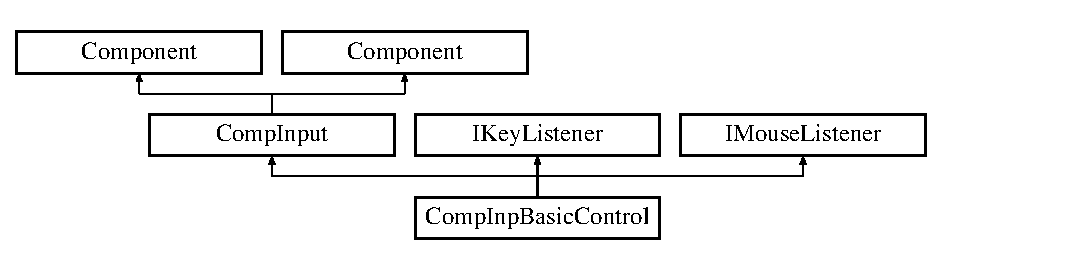
\includegraphics[height=2.978723cm]{class_comp_inp_basic_control}
\end{center}
\end{figure}
\subsection*{Public Member Functions}
\begin{DoxyCompactItemize}
\item 
{\bfseries Comp\+Inp\+Basic\+Control} (\hyperlink{class_i_m_e_h}{I\+M\+EH} $\ast$seh)\hypertarget{class_comp_inp_basic_control_a8ce8cf589006e312635f93e69af47fd7}{}\label{class_comp_inp_basic_control_a8ce8cf589006e312635f93e69af47fd7}

\item 
std\+::string {\bfseries Get\+ID} ()\hypertarget{class_comp_inp_basic_control_ac39216e5350792ddf537bfc4fedd0b3a}{}\label{class_comp_inp_basic_control_ac39216e5350792ddf537bfc4fedd0b3a}

\item 
void {\bfseries on\+Key\+Event} (\hyperlink{union_reb_event}{Reb\+Event} keyevent)\hypertarget{class_comp_inp_basic_control_a76db109690c6bd5be6b5cd128db232f6}{}\label{class_comp_inp_basic_control_a76db109690c6bd5be6b5cd128db232f6}

\item 
void {\bfseries on\+M\+Motion\+Event} (\hyperlink{union_reb_event}{Reb\+Event} mev)\hypertarget{class_comp_inp_basic_control_a104a9df471fe46be6b135ec7ebc79b6b}{}\label{class_comp_inp_basic_control_a104a9df471fe46be6b135ec7ebc79b6b}

\item 
void {\bfseries update} ()\hypertarget{class_comp_inp_basic_control_aa42c5f36ba3a45d98b793da7f0774756}{}\label{class_comp_inp_basic_control_aa42c5f36ba3a45d98b793da7f0774756}

\end{DoxyCompactItemize}
\subsection*{Additional Inherited Members}


The documentation for this class was generated from the following files\+:\begin{DoxyCompactItemize}
\item 
Code/\+Reb\+Entity\+System/Comp\+Input.\+h\item 
Code/\+Reb\+Entity\+System/Comp\+Input.\+cpp\end{DoxyCompactItemize}

\hypertarget{class_comp_inp_key}{}\section{Comp\+Inp\+Key Class Reference}
\label{class_comp_inp_key}\index{Comp\+Inp\+Key@{Comp\+Inp\+Key}}
Inheritance diagram for Comp\+Inp\+Key\+:\begin{figure}[H]
\begin{center}
\leavevmode
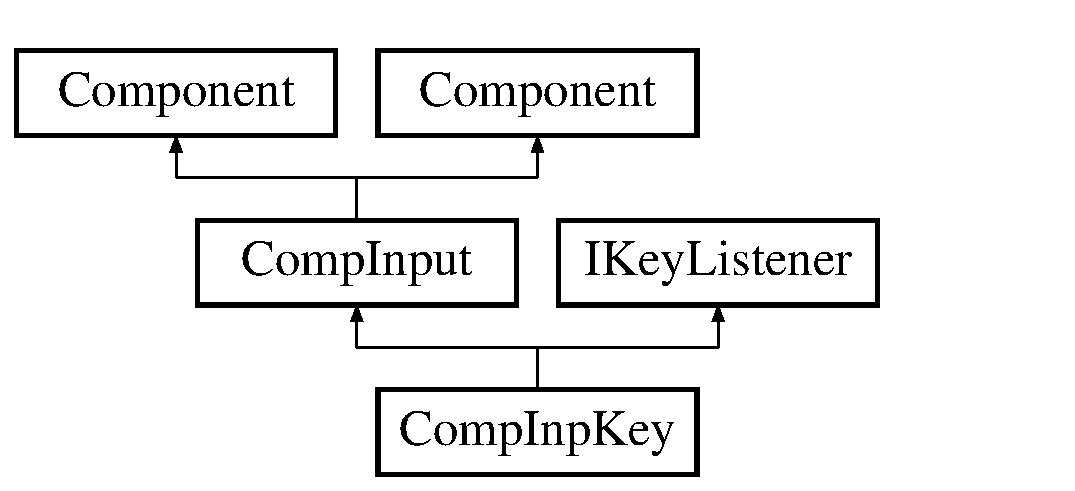
\includegraphics[height=3.000000cm]{class_comp_inp_key}
\end{center}
\end{figure}
\subsection*{Public Member Functions}
\begin{DoxyCompactItemize}
\item 
{\bfseries Comp\+Inp\+Key} (\hyperlink{class_i_m_e_h}{I\+M\+EH} $\ast$sim)\hypertarget{class_comp_inp_key_a30ce505e5adc0b7de796a99fb3370740}{}\label{class_comp_inp_key_a30ce505e5adc0b7de796a99fb3370740}

\item 
std\+::string {\bfseries Get\+ID} ()\hypertarget{class_comp_inp_key_a4229c301203afb531aee44d774396500}{}\label{class_comp_inp_key_a4229c301203afb531aee44d774396500}

\item 
void {\bfseries on\+Key\+Event} (\hyperlink{union_reb_event}{Reb\+Event} $\ast$re)\hypertarget{class_comp_inp_key_aa5c99c1048a2a5dc89863c222fd1cf61}{}\label{class_comp_inp_key_aa5c99c1048a2a5dc89863c222fd1cf61}

\end{DoxyCompactItemize}
\subsection*{Additional Inherited Members}


The documentation for this class was generated from the following file\+:\begin{DoxyCompactItemize}
\item 
Code/\+Reb\+Entity\+System/Reb\+Comps.\+h\end{DoxyCompactItemize}

\hypertarget{class_comp_input}{}\section{Comp\+Input Class Reference}
\label{class_comp_input}\index{Comp\+Input@{Comp\+Input}}
Inheritance diagram for Comp\+Input\+:\begin{figure}[H]
\begin{center}
\leavevmode
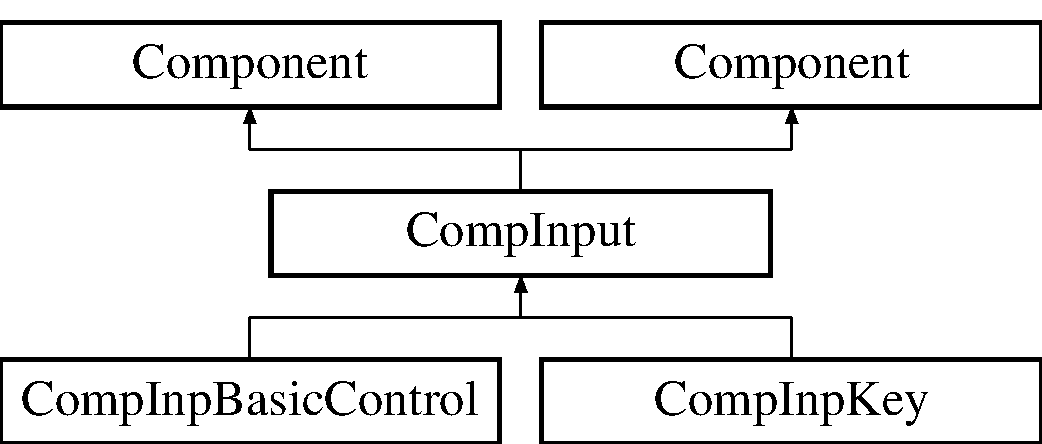
\includegraphics[height=3.000000cm]{class_comp_input}
\end{center}
\end{figure}
\subsection*{Public Member Functions}
\begin{DoxyCompactItemize}
\item 
std\+::string {\bfseries Get\+Type} ()\hypertarget{class_comp_input_af1216a30f938795874dd9a38e6c89345}{}\label{class_comp_input_af1216a30f938795874dd9a38e6c89345}

\item 
std\+::string {\bfseries Get\+Type} ()\hypertarget{class_comp_input_af1216a30f938795874dd9a38e6c89345}{}\label{class_comp_input_af1216a30f938795874dd9a38e6c89345}

\end{DoxyCompactItemize}
\subsection*{Protected Attributes}
\begin{DoxyCompactItemize}
\item 
\hyperlink{class_i_m_e_h}{I\+M\+EH} $\ast$ {\bfseries ievh}\hypertarget{class_comp_input_a99f7be8e318fe4394a300d88c0184e6d}{}\label{class_comp_input_a99f7be8e318fe4394a300d88c0184e6d}

\end{DoxyCompactItemize}


The documentation for this class was generated from the following files\+:\begin{DoxyCompactItemize}
\item 
Code/\+Reb\+Entity\+System/Comp\+Input.\+h\item 
Code/\+Reb\+Entity\+System/Reb\+Comps.\+h\end{DoxyCompactItemize}

\hypertarget{class_comp_phy_model}{}\section{Comp\+Phy\+Model Class Reference}
\label{class_comp_phy_model}\index{Comp\+Phy\+Model@{Comp\+Phy\+Model}}
Inheritance diagram for Comp\+Phy\+Model\+:\begin{figure}[H]
\begin{center}
\leavevmode
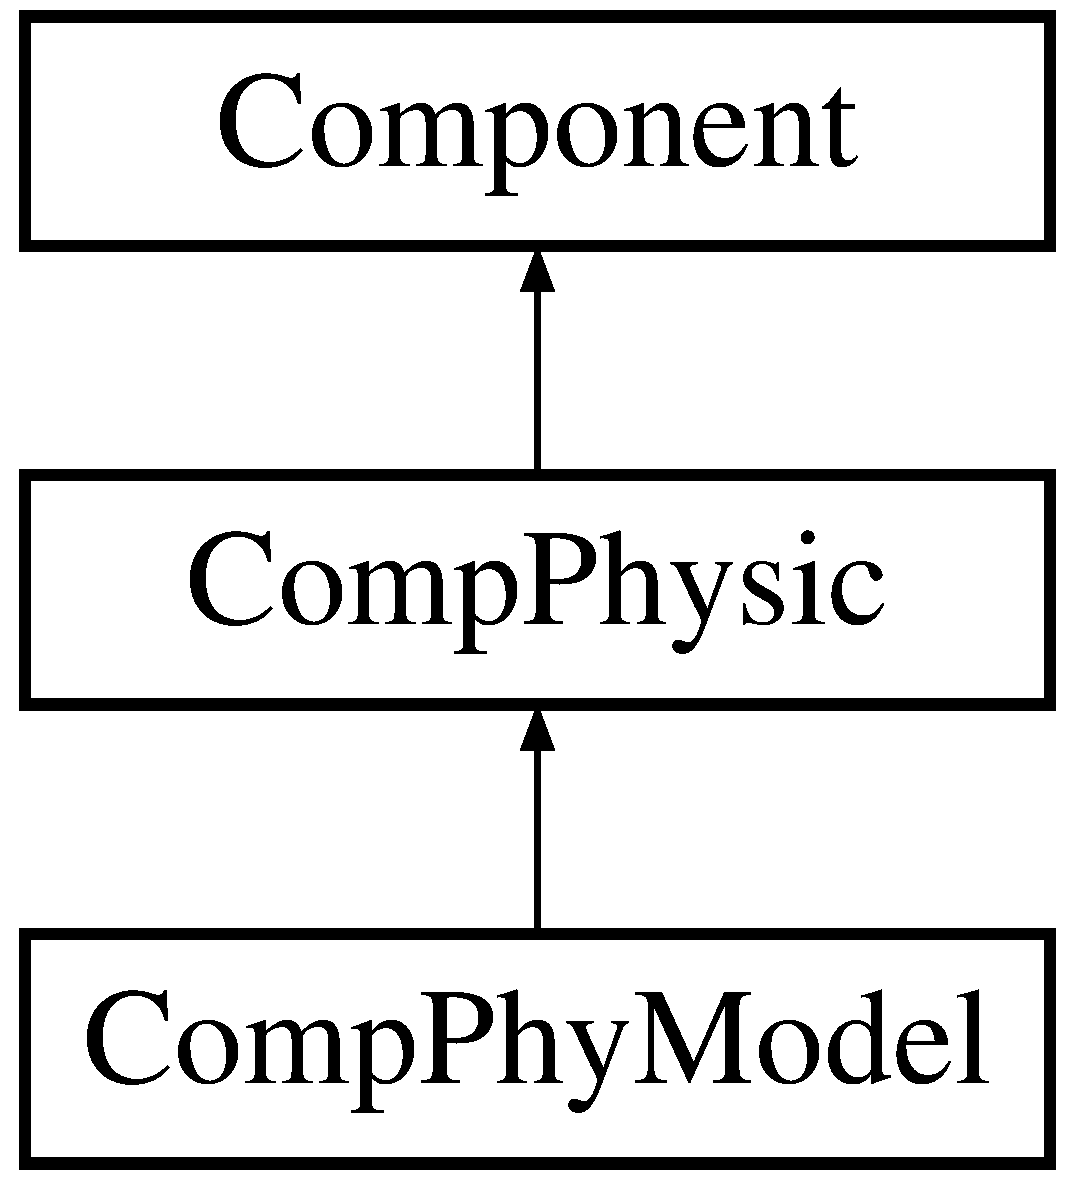
\includegraphics[height=3.000000cm]{class_comp_phy_model}
\end{center}
\end{figure}
\subsection*{Public Member Functions}
\begin{DoxyCompactItemize}
\item 
{\bfseries Comp\+Phy\+Model} (bt\+Dynamics\+World $\ast$S\+DW, \hyperlink{class_i_render_device}{I\+Render\+Device} $\ast$S\+I\+RD, std\+::string smf)\hypertarget{class_comp_phy_model_ab33844f5ba2cecf276af4fad712ad151}{}\label{class_comp_phy_model_ab33844f5ba2cecf276af4fad712ad151}

\item 
void {\bfseries Load\+Physic} ()\hypertarget{class_comp_phy_model_a7739ac89dd8193a8e2f304d73f9bd079}{}\label{class_comp_phy_model_a7739ac89dd8193a8e2f304d73f9bd079}

\item 
void {\bfseries Set\+Physic\+State} (Physic\+State sps)\hypertarget{class_comp_phy_model_a92d33050fb33c0148d7d2d1cc802f67b}{}\label{class_comp_phy_model_a92d33050fb33c0148d7d2d1cc802f67b}

\item 
std\+::string {\bfseries Get\+ID} ()\hypertarget{class_comp_phy_model_a72c0bc83dc4bd8b6611bcf02b7850365}{}\label{class_comp_phy_model_a72c0bc83dc4bd8b6611bcf02b7850365}

\item 
Physic\+State {\bfseries Get\+Physic\+State} ()\hypertarget{class_comp_phy_model_a2c815b9e9b71a0ac2bde394444cb7078}{}\label{class_comp_phy_model_a2c815b9e9b71a0ac2bde394444cb7078}

\end{DoxyCompactItemize}


The documentation for this class was generated from the following files\+:\begin{DoxyCompactItemize}
\item 
Code/\+Reb\+Entity\+System/Comp\+Physics.\+h\item 
Code/\+Reb\+Entity\+System/Comp\+Physics.\+cpp\end{DoxyCompactItemize}

\hypertarget{class_comp_phy_moovable}{}\section{Comp\+Phy\+Moovable Class Reference}
\label{class_comp_phy_moovable}\index{Comp\+Phy\+Moovable@{Comp\+Phy\+Moovable}}
Inheritance diagram for Comp\+Phy\+Moovable\+:\begin{figure}[H]
\begin{center}
\leavevmode
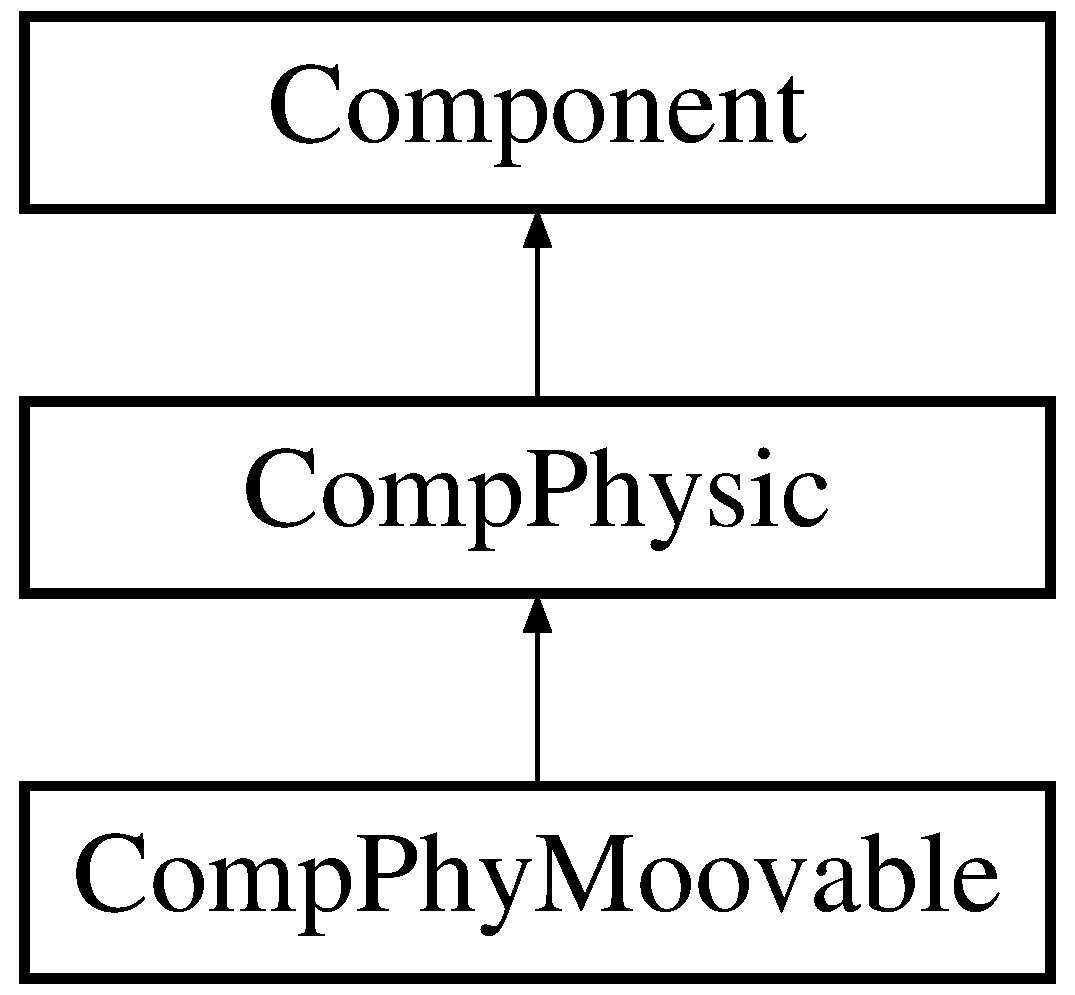
\includegraphics[height=3.000000cm]{class_comp_phy_moovable}
\end{center}
\end{figure}
\subsection*{Public Member Functions}
\begin{DoxyCompactItemize}
\item 
{\bfseries Comp\+Phy\+Moovable} (bt\+Dynamics\+World $\ast$S\+DW)\hypertarget{class_comp_phy_moovable_a9ce47ac288f79aa9901f12166d46574a}{}\label{class_comp_phy_moovable_a9ce47ac288f79aa9901f12166d46574a}

\item 
void {\bfseries Load\+Physic} ()\hypertarget{class_comp_phy_moovable_af1f3236601aa1477b0c06b2fcf49acea}{}\label{class_comp_phy_moovable_af1f3236601aa1477b0c06b2fcf49acea}

\item 
void {\bfseries Set\+R\+VC} (\hyperlink{class_i_vertex_cache}{I\+Vertex\+Cache} $\ast$set)\hypertarget{class_comp_phy_moovable_a5c2635e5f3db3784594c940888bbf741}{}\label{class_comp_phy_moovable_a5c2635e5f3db3784594c940888bbf741}

\item 
std\+::string {\bfseries Get\+ID} ()\hypertarget{class_comp_phy_moovable_a6f6cc50a1e0775c456774fdd9fcf05fc}{}\label{class_comp_phy_moovable_a6f6cc50a1e0775c456774fdd9fcf05fc}

\item 
void {\bfseries update} ()\hypertarget{class_comp_phy_moovable_a595f0cd905cd8bbae94564169e246f5c}{}\label{class_comp_phy_moovable_a595f0cd905cd8bbae94564169e246f5c}

\item 
void {\bfseries Moov} ()\hypertarget{class_comp_phy_moovable_a2b45c9d5000a2c7dbc9890f5f44144b8}{}\label{class_comp_phy_moovable_a2b45c9d5000a2c7dbc9890f5f44144b8}

\end{DoxyCompactItemize}


The documentation for this class was generated from the following file\+:\begin{DoxyCompactItemize}
\item 
Code/\+Reb\+Entity\+System/Comp\+Physics.\+h\end{DoxyCompactItemize}

\hypertarget{class_comp_physic}{}\section{Comp\+Physic Class Reference}
\label{class_comp_physic}\index{Comp\+Physic@{Comp\+Physic}}
Inheritance diagram for Comp\+Physic\+:\begin{figure}[H]
\begin{center}
\leavevmode
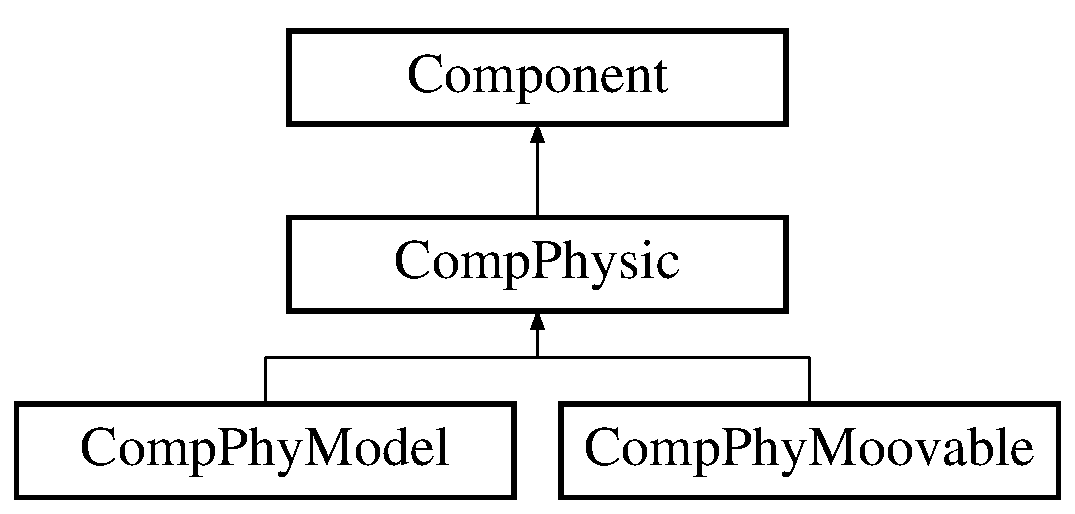
\includegraphics[height=3.000000cm]{class_comp_physic}
\end{center}
\end{figure}
\subsection*{Public Member Functions}
\begin{DoxyCompactItemize}
\item 
std\+::string {\bfseries Get\+Type} ()\hypertarget{class_comp_physic_a56af12ce4e88c8e4edc0e7f07bd7d1a0}{}\label{class_comp_physic_a56af12ce4e88c8e4edc0e7f07bd7d1a0}

\end{DoxyCompactItemize}


The documentation for this class was generated from the following file\+:\begin{DoxyCompactItemize}
\item 
Code/\+Reb\+Entity\+System/Comp\+Physics.\+h\end{DoxyCompactItemize}

\hypertarget{class_comp_vis_model}{}\section{Comp\+Vis\+Model Class Reference}
\label{class_comp_vis_model}\index{Comp\+Vis\+Model@{Comp\+Vis\+Model}}
Inheritance diagram for Comp\+Vis\+Model\+:\begin{figure}[H]
\begin{center}
\leavevmode
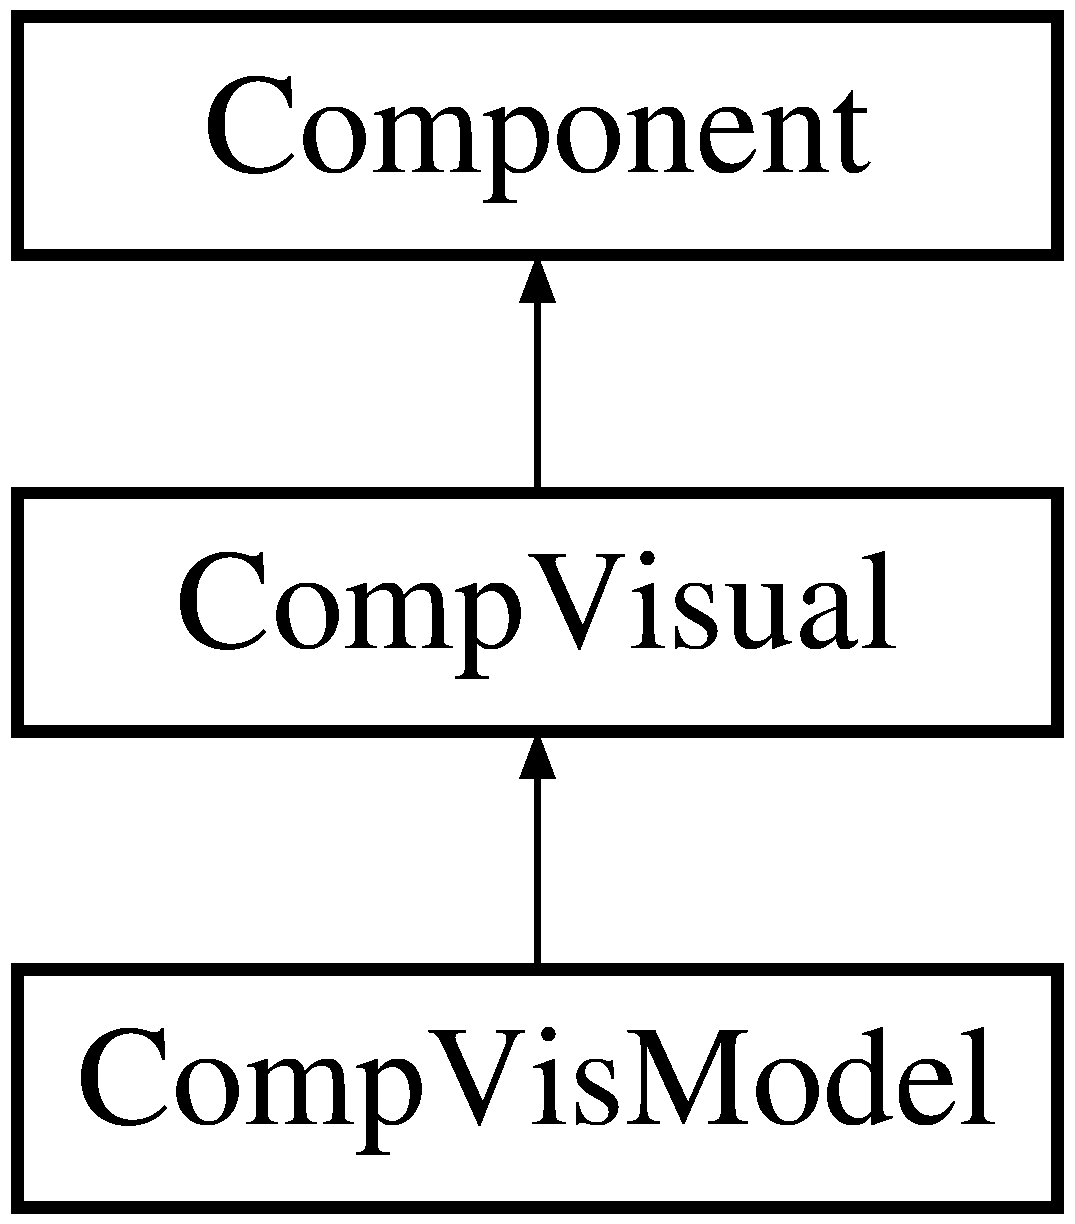
\includegraphics[height=3.000000cm]{class_comp_vis_model}
\end{center}
\end{figure}
\subsection*{Public Member Functions}
\begin{DoxyCompactItemize}
\item 
{\bfseries Comp\+Vis\+Model} (\hyperlink{class_i_render_device}{I\+Render\+Device} $\ast$sird, \hyperlink{class_reb_file_system}{Reb\+File\+System} $\ast$srfs)\hypertarget{class_comp_vis_model_a339383004ab2d165964a4e7c7927e8b4}{}\label{class_comp_vis_model_a339383004ab2d165964a4e7c7927e8b4}

\item 
void {\bfseries update} ()\hypertarget{class_comp_vis_model_a550eee5395e9c3caa59e4b6f22f781a0}{}\label{class_comp_vis_model_a550eee5395e9c3caa59e4b6f22f781a0}

\item 
void {\bfseries Load\+Model} (std\+::string filename)\hypertarget{class_comp_vis_model_a2f534d09a99504b65fd4da7219bccc34}{}\label{class_comp_vis_model_a2f534d09a99504b65fd4da7219bccc34}

\item 
std\+::string {\bfseries Get\+ID} ()\hypertarget{class_comp_vis_model_a9259963810adc0cb523f47e2ff36b7cd}{}\label{class_comp_vis_model_a9259963810adc0cb523f47e2ff36b7cd}

\end{DoxyCompactItemize}
\subsection*{Additional Inherited Members}


The documentation for this class was generated from the following files\+:\begin{DoxyCompactItemize}
\item 
Code/\+Reb\+Entity\+System/Comp\+Visual.\+h\item 
Code/\+Reb\+Entity\+System/Comp\+Visual.\+cpp\end{DoxyCompactItemize}

\hypertarget{class_comp_vis_terrain}{}\section{Comp\+Vis\+Terrain Class Reference}
\label{class_comp_vis_terrain}\index{Comp\+Vis\+Terrain@{Comp\+Vis\+Terrain}}
Inheritance diagram for Comp\+Vis\+Terrain\+:\begin{figure}[H]
\begin{center}
\leavevmode
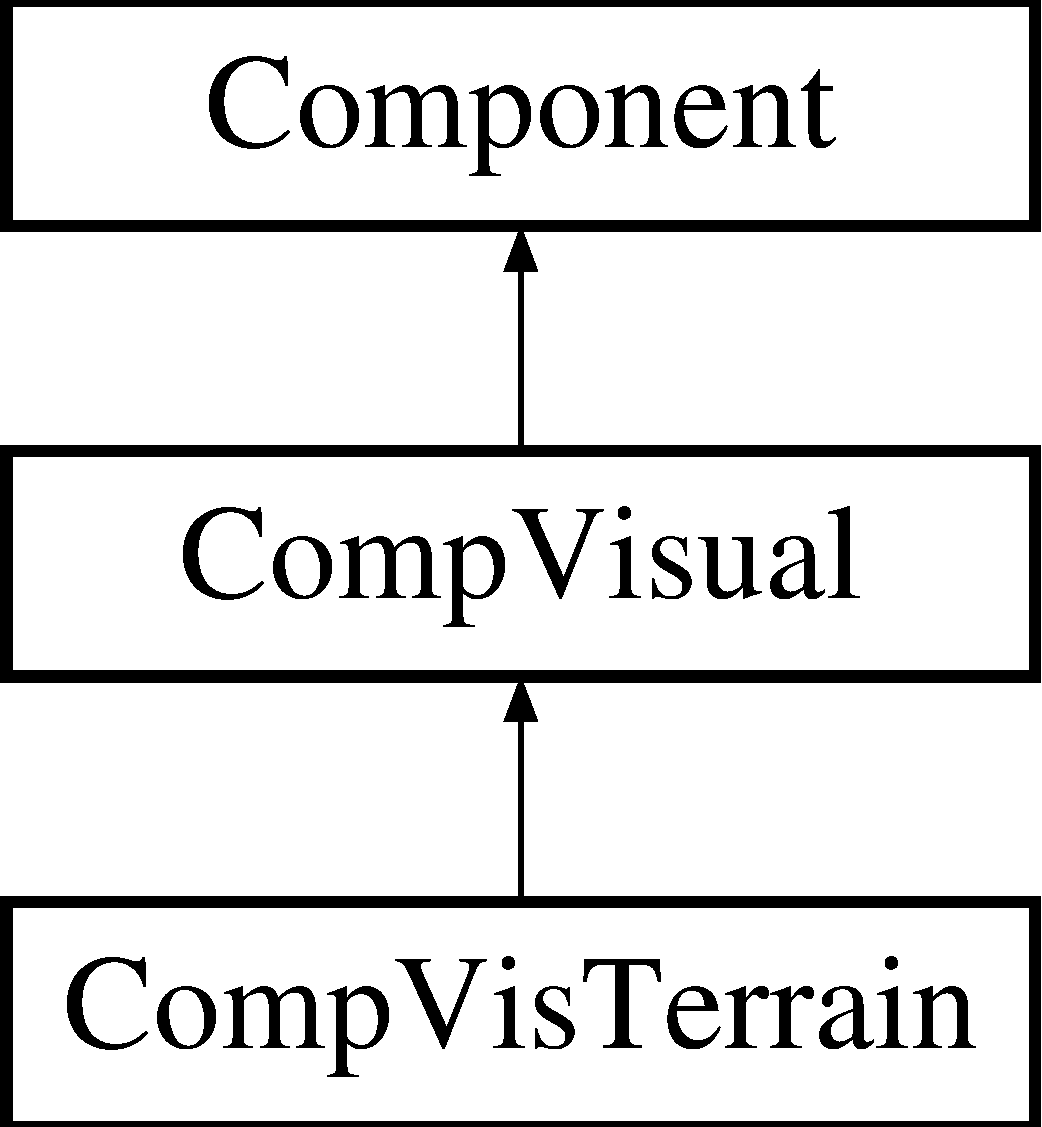
\includegraphics[height=3.000000cm]{class_comp_vis_terrain}
\end{center}
\end{figure}
\subsection*{Public Member Functions}
\begin{DoxyCompactItemize}
\item 
{\bfseries Comp\+Vis\+Terrain} (\hyperlink{class_i_render_device}{I\+Render\+Device} $\ast$sird)\hypertarget{class_comp_vis_terrain_a3af611d50cfab9e943cf1d24591e0ad0}{}\label{class_comp_vis_terrain_a3af611d50cfab9e943cf1d24591e0ad0}

\item 
void {\bfseries update} ()\hypertarget{class_comp_vis_terrain_a3ce6d6f6aa7890cf8ed626e24a635c0a}{}\label{class_comp_vis_terrain_a3ce6d6f6aa7890cf8ed626e24a635c0a}

\item 
void {\bfseries Create\+Terrain} ()\hypertarget{class_comp_vis_terrain_a3350c4fa08f262a48d898ecd572f1f05}{}\label{class_comp_vis_terrain_a3350c4fa08f262a48d898ecd572f1f05}

\item 
std\+::string {\bfseries Get\+ID} ()\hypertarget{class_comp_vis_terrain_abed1a415813689541b660966770fc5b2}{}\label{class_comp_vis_terrain_abed1a415813689541b660966770fc5b2}

\end{DoxyCompactItemize}
\subsection*{Additional Inherited Members}


The documentation for this class was generated from the following files\+:\begin{DoxyCompactItemize}
\item 
Code/\+Reb\+Entity\+System/Comp\+Visual.\+h\item 
Code/\+Reb\+Entity\+System/Comp\+Vis\+Terrain.\+cpp\end{DoxyCompactItemize}

\hypertarget{class_comp_visual}{}\section{Comp\+Visual Class Reference}
\label{class_comp_visual}\index{Comp\+Visual@{Comp\+Visual}}
Inheritance diagram for Comp\+Visual\+:\begin{figure}[H]
\begin{center}
\leavevmode
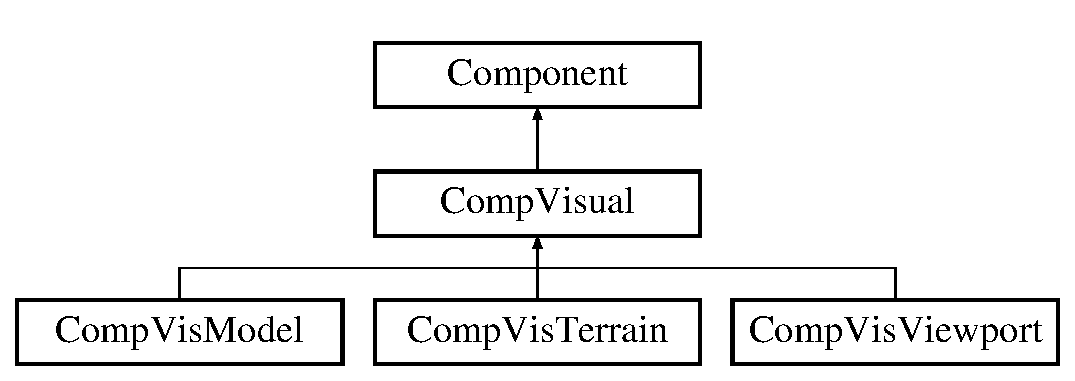
\includegraphics[height=3.000000cm]{class_comp_visual}
\end{center}
\end{figure}
\subsection*{Public Member Functions}
\begin{DoxyCompactItemize}
\item 
std\+::string {\bfseries Get\+Type} ()\hypertarget{class_comp_visual_a87b320b011374cccf8e69b64f1d74fb9}{}\label{class_comp_visual_a87b320b011374cccf8e69b64f1d74fb9}

\end{DoxyCompactItemize}
\subsection*{Protected Attributes}
\begin{DoxyCompactItemize}
\item 
\hyperlink{class_i_render_device}{I\+Render\+Device} $\ast$ {\bfseries I\+RD}\hypertarget{class_comp_visual_aa0050d76d0d62fa914411576595e89d6}{}\label{class_comp_visual_aa0050d76d0d62fa914411576595e89d6}

\item 
\hyperlink{class_i_vertex_cache}{I\+Vertex\+Cache} $\ast$ {\bfseries rvc}\hypertarget{class_comp_visual_aa04522ccdab76a9e26f687290dd43d2c}{}\label{class_comp_visual_aa04522ccdab76a9e26f687290dd43d2c}

\end{DoxyCompactItemize}


The documentation for this class was generated from the following file\+:\begin{DoxyCompactItemize}
\item 
Code/\+Reb\+Entity\+System/Comp\+Visual.\+h\end{DoxyCompactItemize}

\hypertarget{class_comp_vis_viewport}{}\section{Comp\+Vis\+Viewport Class Reference}
\label{class_comp_vis_viewport}\index{Comp\+Vis\+Viewport@{Comp\+Vis\+Viewport}}
Inheritance diagram for Comp\+Vis\+Viewport\+:\begin{figure}[H]
\begin{center}
\leavevmode
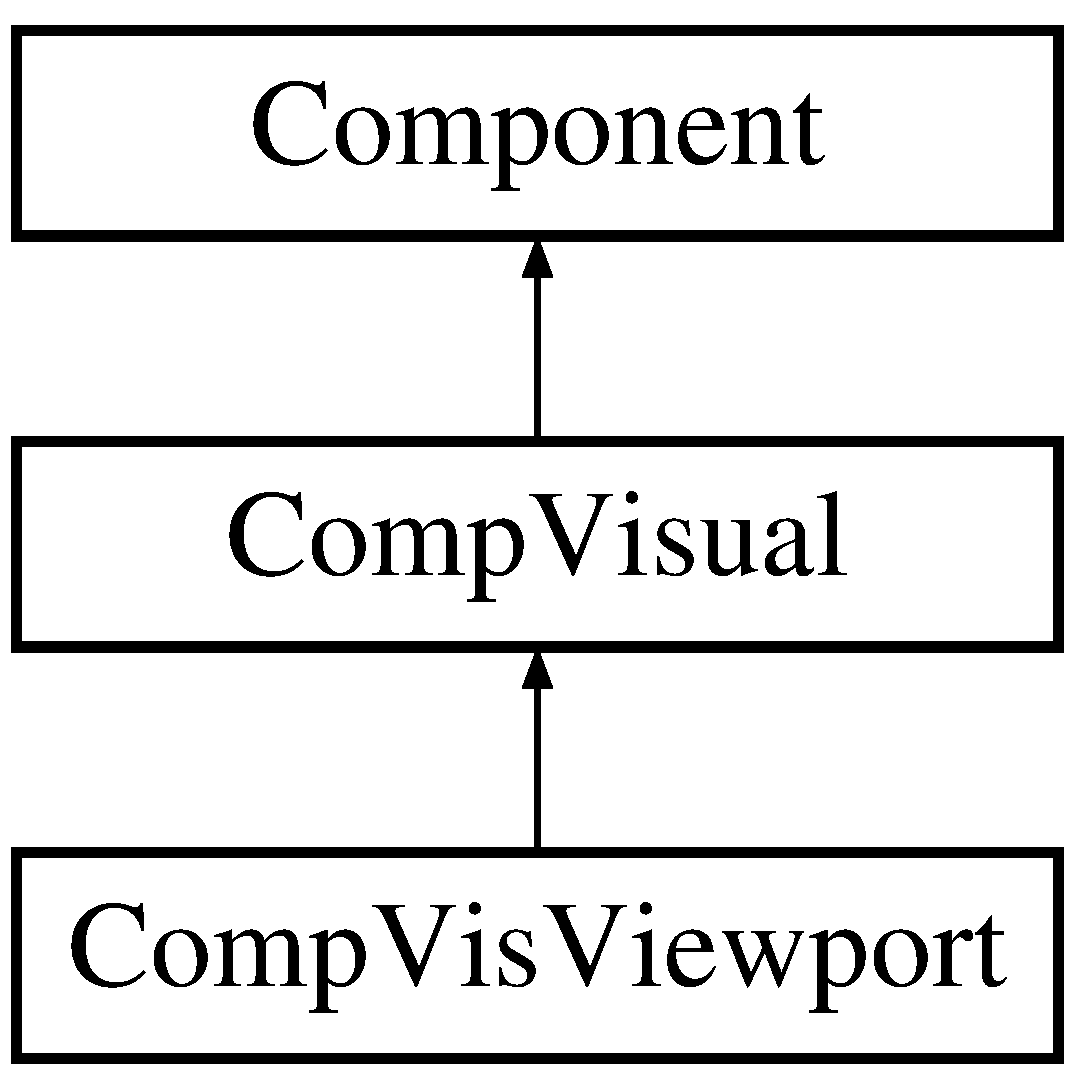
\includegraphics[height=3.000000cm]{class_comp_vis_viewport}
\end{center}
\end{figure}
\subsection*{Public Member Functions}
\begin{DoxyCompactItemize}
\item 
{\bfseries Comp\+Vis\+Viewport} (\hyperlink{class_i_render_device}{I\+Render\+Device} $\ast$S\+I\+RD)\hypertarget{class_comp_vis_viewport_a1b86479fcbeb97248df7a2d061900fe1}{}\label{class_comp_vis_viewport_a1b86479fcbeb97248df7a2d061900fe1}

\item 
void {\bfseries update} ()\hypertarget{class_comp_vis_viewport_aa974c63d605e3ebc957f7ce18220a3f4}{}\label{class_comp_vis_viewport_aa974c63d605e3ebc957f7ce18220a3f4}

\item 
std\+::string {\bfseries Get\+ID} ()\hypertarget{class_comp_vis_viewport_a93e1dcc65e38f028323a5685cfac50cd}{}\label{class_comp_vis_viewport_a93e1dcc65e38f028323a5685cfac50cd}

\item 
void {\bfseries Set\+Active\+Viewport} ()\hypertarget{class_comp_vis_viewport_a4371621bdf3d252c66f2e2b2b6d01804}{}\label{class_comp_vis_viewport_a4371621bdf3d252c66f2e2b2b6d01804}

\end{DoxyCompactItemize}
\subsection*{Additional Inherited Members}


The documentation for this class was generated from the following files\+:\begin{DoxyCompactItemize}
\item 
Code/\+Reb\+Entity\+System/Comp\+Visual.\+h\item 
Code/\+Reb\+Entity\+System/Comp\+Visual.\+cpp\end{DoxyCompactItemize}

\hypertarget{class_c_s_m}{}\section{C\+SM Class Reference}
\label{class_c_s_m}\index{C\+SM@{C\+SM}}
Inheritance diagram for C\+SM\+:\begin{figure}[H]
\begin{center}
\leavevmode
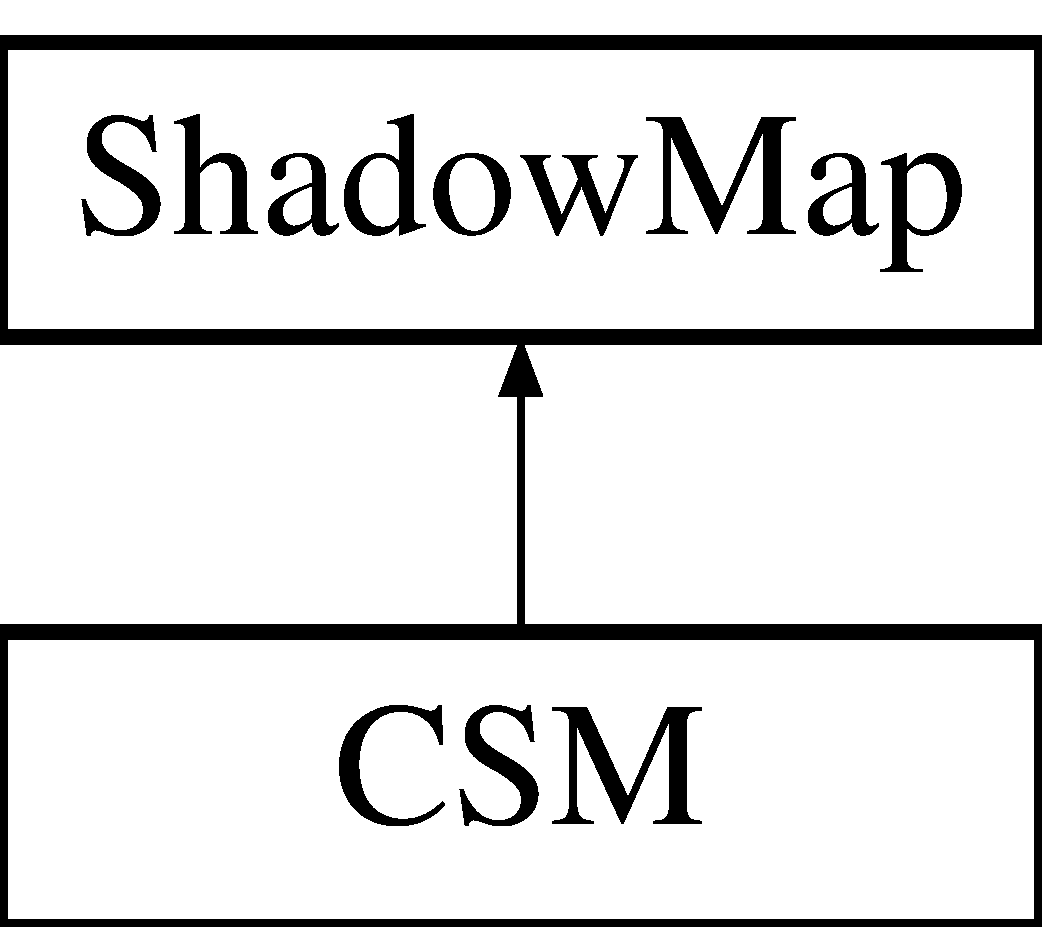
\includegraphics[height=2.000000cm]{class_c_s_m}
\end{center}
\end{figure}
\subsection*{Public Member Functions}
\begin{DoxyCompactItemize}
\item 
void {\bfseries Set\+S\+Params} (G\+Luint handle)\hypertarget{class_c_s_m_a4a9ef3a9dc40e048ef7953275d199578}{}\label{class_c_s_m_a4a9ef3a9dc40e048ef7953275d199578}

\item 
void {\bfseries Write} ()\hypertarget{class_c_s_m_aa376ce3b0114beac9c72c437db4f56fe}{}\label{class_c_s_m_aa376ce3b0114beac9c72c437db4f56fe}

\item 
void {\bfseries Read} ()\hypertarget{class_c_s_m_a129f8db031142948042b96e1310466c6}{}\label{class_c_s_m_a129f8db031142948042b96e1310466c6}

\item 
void \hyperlink{class_c_s_m_ad33a5634ccf4af01fbf336cf54b0b0bc}{Shadow\+Pass} ()
\end{DoxyCompactItemize}
\subsection*{Additional Inherited Members}


\subsection{Member Function Documentation}
\index{C\+SM@{C\+SM}!Shadow\+Pass@{Shadow\+Pass}}
\index{Shadow\+Pass@{Shadow\+Pass}!C\+SM@{C\+SM}}
\subsubsection[{\texorpdfstring{Shadow\+Pass()}{ShadowPass()}}]{\setlength{\rightskip}{0pt plus 5cm}void C\+S\+M\+::\+Shadow\+Pass (
\begin{DoxyParamCaption}
{}
\end{DoxyParamCaption}
)\hspace{0.3cm}{\ttfamily [virtual]}}\hypertarget{class_c_s_m_ad33a5634ccf4af01fbf336cf54b0b0bc}{}\label{class_c_s_m_ad33a5634ccf4af01fbf336cf54b0b0bc}

\begin{DoxyItemize}
\item shadowmat.\+Inverse\+Of(shadowmat);$\ast$/ 
\end{DoxyItemize}

Implements \hyperlink{class_shadow_map}{Shadow\+Map}.



The documentation for this class was generated from the following files\+:\begin{DoxyCompactItemize}
\item 
Code/\+Reb\+G\+L/Reb\+G\+L\+\_\+\+Light\+System.\+h\item 
Code/\+Reb\+G\+L/Reb\+G\+L\+\_\+\+Light\+System.\+cpp\end{DoxyCompactItemize}

\hypertarget{classtinyxml2_1_1_dyn_array}{}\section{tinyxml2\+:\+:Dyn\+Array$<$ T, I\+N\+IT $>$ Class Template Reference}
\label{classtinyxml2_1_1_dyn_array}\index{tinyxml2\+::\+Dyn\+Array$<$ T, I\+N\+I\+T $>$@{tinyxml2\+::\+Dyn\+Array$<$ T, I\+N\+I\+T $>$}}
\subsection*{Public Member Functions}
\begin{DoxyCompactItemize}
\item 
void {\bfseries Clear} ()\hypertarget{classtinyxml2_1_1_dyn_array_a9c3bb53e7091804924639bb6690d763d}{}\label{classtinyxml2_1_1_dyn_array_a9c3bb53e7091804924639bb6690d763d}

\item 
void {\bfseries Push} (T t)\hypertarget{classtinyxml2_1_1_dyn_array_a498de53808ba0151fef54ea10bf51050}{}\label{classtinyxml2_1_1_dyn_array_a498de53808ba0151fef54ea10bf51050}

\item 
T $\ast$ {\bfseries Push\+Arr} (int count)\hypertarget{classtinyxml2_1_1_dyn_array_aa3c360d40addc3b05121da9f60a01b4d}{}\label{classtinyxml2_1_1_dyn_array_aa3c360d40addc3b05121da9f60a01b4d}

\item 
T {\bfseries Pop} ()\hypertarget{classtinyxml2_1_1_dyn_array_a2281e3342bc235bf391a67e362c75866}{}\label{classtinyxml2_1_1_dyn_array_a2281e3342bc235bf391a67e362c75866}

\item 
void {\bfseries Pop\+Arr} (int count)\hypertarget{classtinyxml2_1_1_dyn_array_ab45c0836d8c0260a5b9eda7da80de71c}{}\label{classtinyxml2_1_1_dyn_array_ab45c0836d8c0260a5b9eda7da80de71c}

\item 
bool {\bfseries Empty} () const \hypertarget{classtinyxml2_1_1_dyn_array_a080dc4dc68713964bb17745d4c833158}{}\label{classtinyxml2_1_1_dyn_array_a080dc4dc68713964bb17745d4c833158}

\item 
T \& {\bfseries operator\mbox{[}$\,$\mbox{]}} (int i)\hypertarget{classtinyxml2_1_1_dyn_array_a775a6ab4d41f0eb15bdd863d408dd58f}{}\label{classtinyxml2_1_1_dyn_array_a775a6ab4d41f0eb15bdd863d408dd58f}

\item 
const T \& {\bfseries operator\mbox{[}$\,$\mbox{]}} (int i) const \hypertarget{classtinyxml2_1_1_dyn_array_a1f4874c2608cbd68be1627fca9efd820}{}\label{classtinyxml2_1_1_dyn_array_a1f4874c2608cbd68be1627fca9efd820}

\item 
const T \& {\bfseries Peek\+Top} () const \hypertarget{classtinyxml2_1_1_dyn_array_a9c2282ea8901b5a92ccaac2e6166a788}{}\label{classtinyxml2_1_1_dyn_array_a9c2282ea8901b5a92ccaac2e6166a788}

\item 
int {\bfseries Size} () const \hypertarget{classtinyxml2_1_1_dyn_array_a1299b257b62ea6b4983c488867f219b0}{}\label{classtinyxml2_1_1_dyn_array_a1299b257b62ea6b4983c488867f219b0}

\item 
int {\bfseries Capacity} () const \hypertarget{classtinyxml2_1_1_dyn_array_a8edbe90ed53b2e46b1b5cf53b261e4e7}{}\label{classtinyxml2_1_1_dyn_array_a8edbe90ed53b2e46b1b5cf53b261e4e7}

\item 
const T $\ast$ {\bfseries Mem} () const \hypertarget{classtinyxml2_1_1_dyn_array_a1f39330daeb97d3d1dc3fc12dcf7ac67}{}\label{classtinyxml2_1_1_dyn_array_a1f39330daeb97d3d1dc3fc12dcf7ac67}

\item 
T $\ast$ {\bfseries Mem} ()\hypertarget{classtinyxml2_1_1_dyn_array_a0e0d60b399d54fad5b33d5008bc59c8e}{}\label{classtinyxml2_1_1_dyn_array_a0e0d60b399d54fad5b33d5008bc59c8e}

\end{DoxyCompactItemize}


The documentation for this class was generated from the following file\+:\begin{DoxyCompactItemize}
\item 
Code/\+Reb\+Support/tinyxml2.\+h\end{DoxyCompactItemize}

\hypertarget{class_editor}{}\section{Editor Class Reference}
\label{class_editor}\index{Editor@{Editor}}
Inheritance diagram for Editor\+:\begin{figure}[H]
\begin{center}
\leavevmode
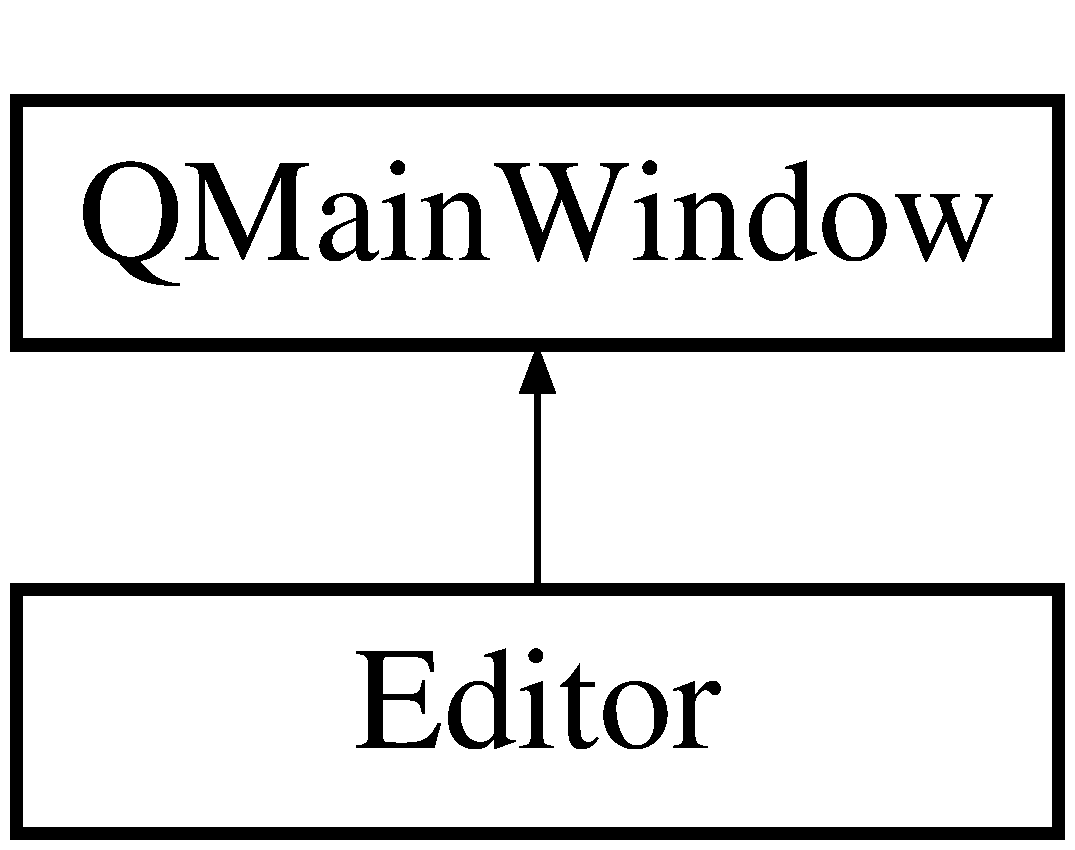
\includegraphics[height=2.000000cm]{class_editor}
\end{center}
\end{figure}
\subsection*{Classes}
\begin{DoxyCompactItemize}
\item 
class \hyperlink{class_editor_1_1_form1}{Form1}
\item 
class \hyperlink{class_editor_1_1_g_l_control}{G\+L\+Control}
\item 
class \hyperlink{class_editor_1_1_open_g_l}{Open\+GL}
\item 
class {\bfseries Program}
\end{DoxyCompactItemize}
\subsection*{Public Member Functions}
\begin{DoxyCompactItemize}
\item 
{\bfseries Editor} (Q\+Widget $\ast$parent=0)\hypertarget{class_editor_a2918aceeffbc123a96e201b0934b9b16}{}\label{class_editor_a2918aceeffbc123a96e201b0934b9b16}

\end{DoxyCompactItemize}


The documentation for this class was generated from the following files\+:\begin{DoxyCompactItemize}
\item 
Code/\+Editor/editor.\+h\item 
Code/\+Editor/editor.\+cpp\end{DoxyCompactItemize}

\hypertarget{class_ui_1_1_editor_class}{}\section{Ui\+:\+:Editor\+Class Class Reference}
\label{class_ui_1_1_editor_class}\index{Ui\+::\+Editor\+Class@{Ui\+::\+Editor\+Class}}
Inheritance diagram for Ui\+:\+:Editor\+Class\+:\begin{figure}[H]
\begin{center}
\leavevmode
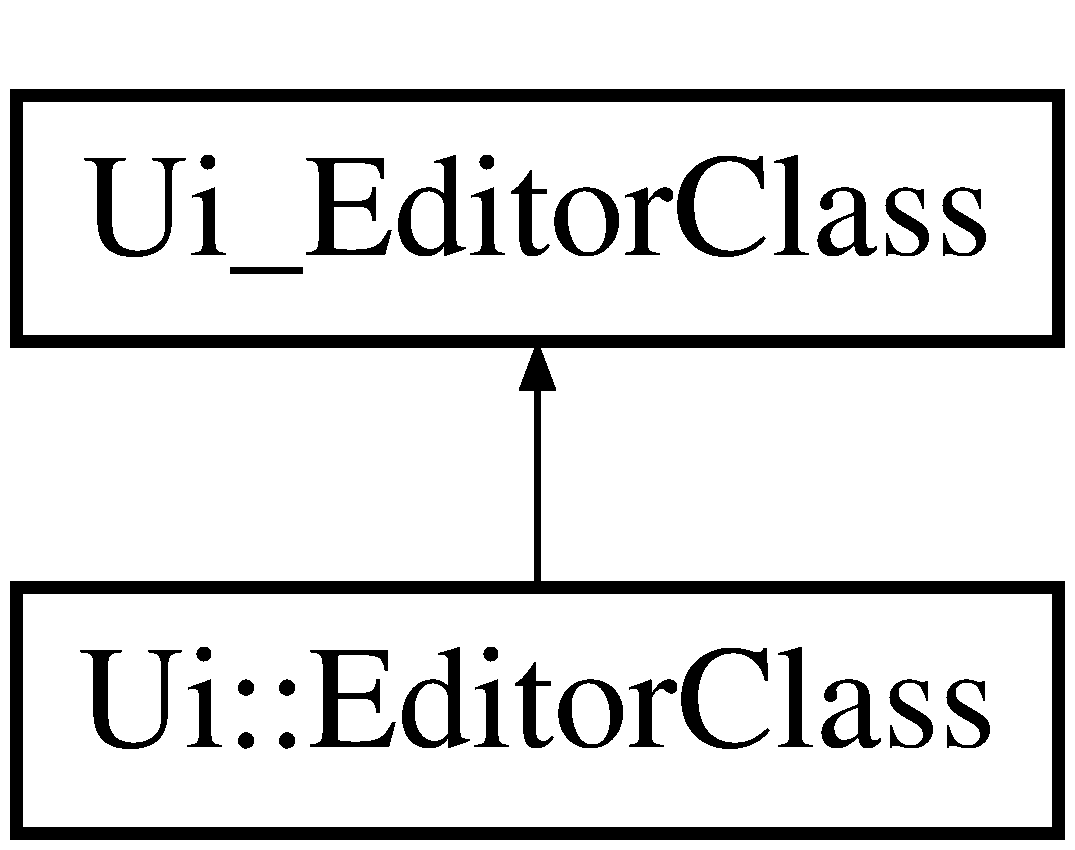
\includegraphics[height=2.000000cm]{class_ui_1_1_editor_class}
\end{center}
\end{figure}
\subsection*{Additional Inherited Members}


The documentation for this class was generated from the following file\+:\begin{DoxyCompactItemize}
\item 
Code/\+Editor/\+Generated\+Files/ui\+\_\+editor.\+h\end{DoxyCompactItemize}

\hypertarget{structtinyxml2_1_1_entity}{}\section{tinyxml2\+:\+:Entity Struct Reference}
\label{structtinyxml2_1_1_entity}\index{tinyxml2\+::\+Entity@{tinyxml2\+::\+Entity}}
\subsection*{Public Attributes}
\begin{DoxyCompactItemize}
\item 
const char $\ast$ {\bfseries pattern}\hypertarget{structtinyxml2_1_1_entity_ab330f5d665d29bfc811ecfa76315894b}{}\label{structtinyxml2_1_1_entity_ab330f5d665d29bfc811ecfa76315894b}

\item 
int {\bfseries length}\hypertarget{structtinyxml2_1_1_entity_a25e2b57cb59cb4fa68f283d7cb570f21}{}\label{structtinyxml2_1_1_entity_a25e2b57cb59cb4fa68f283d7cb570f21}

\item 
char {\bfseries value}\hypertarget{structtinyxml2_1_1_entity_a7334e81e33b4615655a403711b24f3ed}{}\label{structtinyxml2_1_1_entity_a7334e81e33b4615655a403711b24f3ed}

\end{DoxyCompactItemize}


The documentation for this struct was generated from the following file\+:\begin{DoxyCompactItemize}
\item 
Code/\+Reb\+Support/tinyxml2.\+cpp\end{DoxyCompactItemize}

\hypertarget{class_editor_1_1_form1}{}\section{Editor.\+Form1 Class Reference}
\label{class_editor_1_1_form1}\index{Editor.\+Form1@{Editor.\+Form1}}
Inheritance diagram for Editor.\+Form1\+:\begin{figure}[H]
\begin{center}
\leavevmode
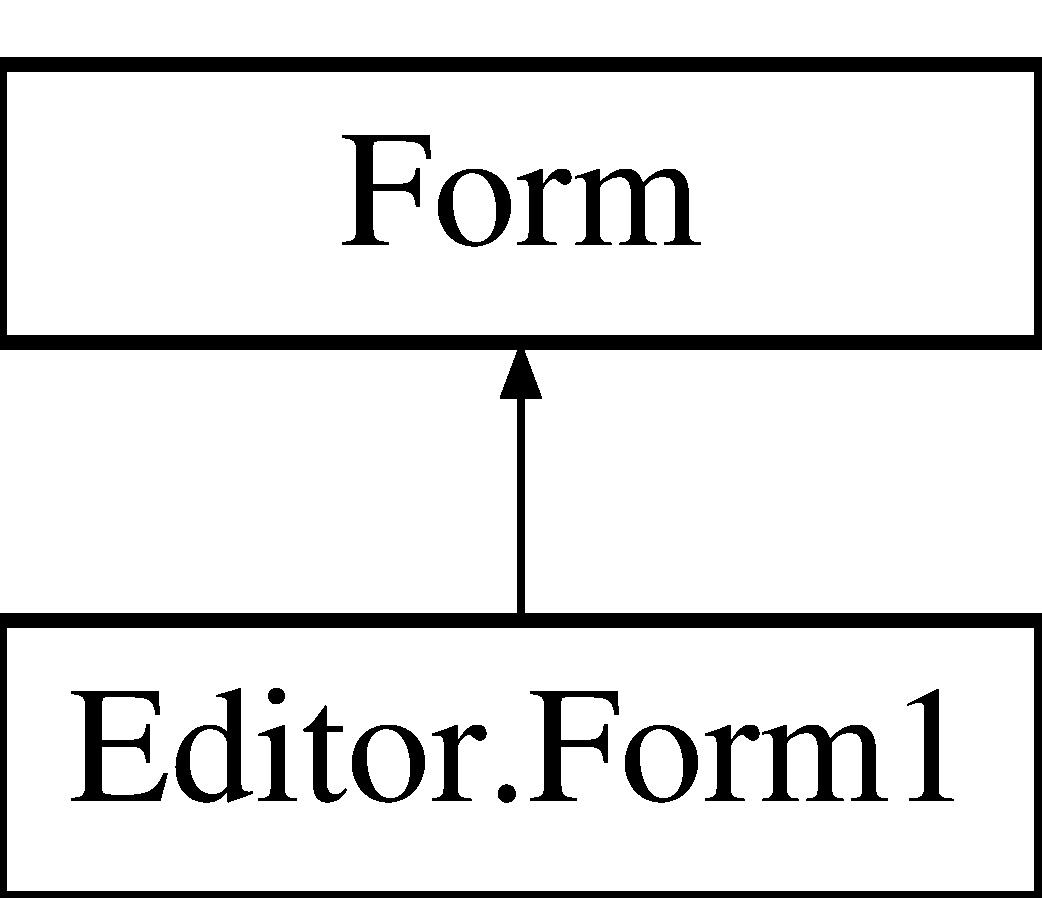
\includegraphics[height=2.000000cm]{class_editor_1_1_form1}
\end{center}
\end{figure}
\subsection*{Protected Member Functions}
\begin{DoxyCompactItemize}
\item 
override void \hyperlink{class_editor_1_1_form1_af599aac279610c185250f2dc294043bc}{Dispose} (bool disposing)
\begin{DoxyCompactList}\small\item\em Clean up any resources being used. \end{DoxyCompactList}\end{DoxyCompactItemize}


\subsection{Member Function Documentation}
\index{Editor\+::\+Form1@{Editor\+::\+Form1}!Dispose@{Dispose}}
\index{Dispose@{Dispose}!Editor\+::\+Form1@{Editor\+::\+Form1}}
\subsubsection[{\texorpdfstring{Dispose(bool disposing)}{Dispose(bool disposing)}}]{\setlength{\rightskip}{0pt plus 5cm}override void Editor.\+Form1.\+Dispose (
\begin{DoxyParamCaption}
\item[{bool}]{disposing}
\end{DoxyParamCaption}
)\hspace{0.3cm}{\ttfamily [inline]}, {\ttfamily [protected]}}\hypertarget{class_editor_1_1_form1_af599aac279610c185250f2dc294043bc}{}\label{class_editor_1_1_form1_af599aac279610c185250f2dc294043bc}


Clean up any resources being used. 


\begin{DoxyParams}{Parameters}
{\em disposing} & true if managed resources should be disposed; otherwise, false.\\
\hline
\end{DoxyParams}


The documentation for this class was generated from the following files\+:\begin{DoxyCompactItemize}
\item 
Code/\+Editor/Form1.\+cs\item 
Code/\+Editor/Form1.\+Designer.\+cs\end{DoxyCompactItemize}

\hypertarget{class_editor_1_1_g_l_control}{}\section{Editor.\+G\+L\+Control Class Reference}
\label{class_editor_1_1_g_l_control}\index{Editor.\+G\+L\+Control@{Editor.\+G\+L\+Control}}
Inheritance diagram for Editor.\+G\+L\+Control\+:\begin{figure}[H]
\begin{center}
\leavevmode
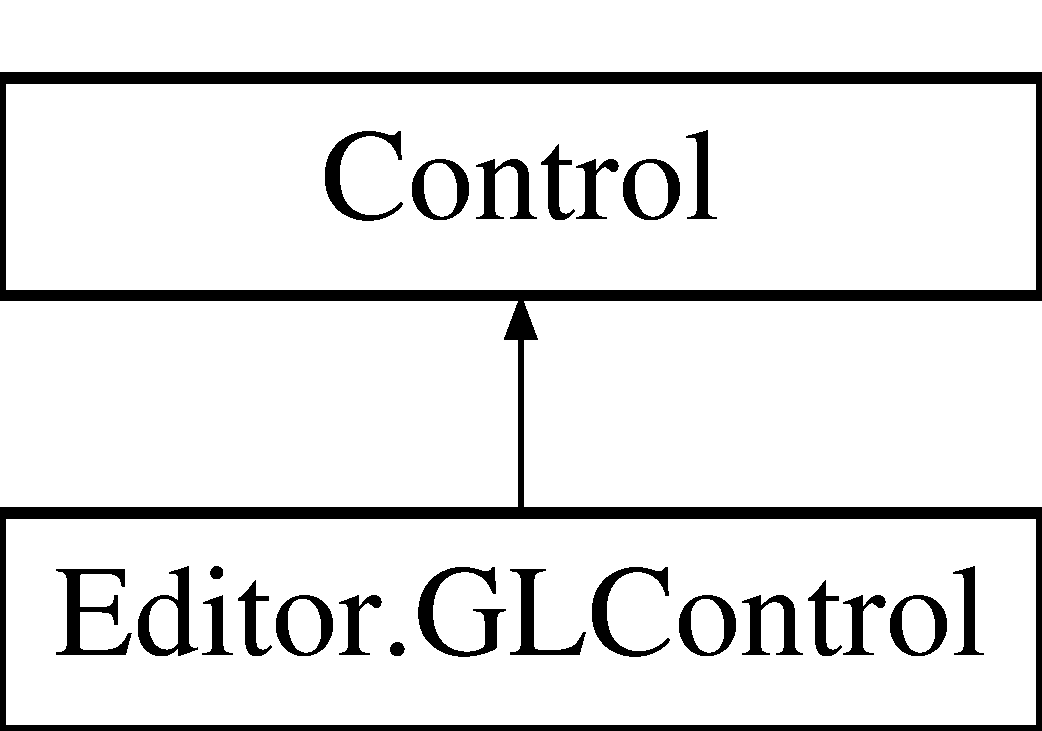
\includegraphics[height=2.000000cm]{class_editor_1_1_g_l_control}
\end{center}
\end{figure}
\subsection*{Public Member Functions}
\begin{DoxyCompactItemize}
\item 
void {\bfseries Draw} ()\hypertarget{class_editor_1_1_g_l_control_aba9a36eab568a716ac0d6da09d24ad7b}{}\label{class_editor_1_1_g_l_control_aba9a36eab568a716ac0d6da09d24ad7b}

\end{DoxyCompactItemize}


The documentation for this class was generated from the following file\+:\begin{DoxyCompactItemize}
\item 
Code/\+Editor/G\+L\+Control.\+cs\end{DoxyCompactItemize}

\hypertarget{class_i_audio_device}{}\section{I\+Audio\+Device Class Reference}
\label{class_i_audio_device}\index{I\+Audio\+Device@{I\+Audio\+Device}}
Inheritance diagram for I\+Audio\+Device\+:\begin{figure}[H]
\begin{center}
\leavevmode
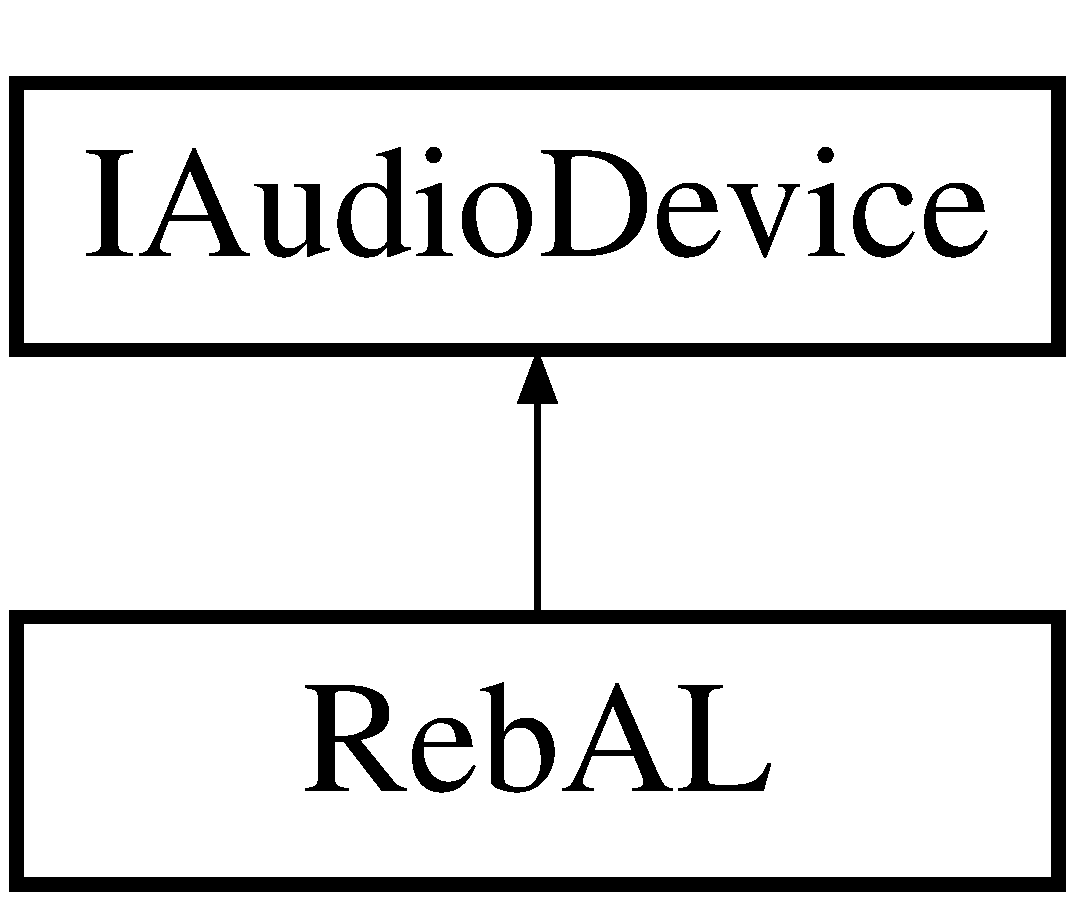
\includegraphics[height=2.000000cm]{class_i_audio_device}
\end{center}
\end{figure}
\subsection*{Public Member Functions}
\begin{DoxyCompactItemize}
\item 
virtual void {\bfseries Init} ()=0\hypertarget{class_i_audio_device_ab819d541358d62bfa59b2302b1d1f765}{}\label{class_i_audio_device_ab819d541358d62bfa59b2302b1d1f765}

\item 
virtual void {\bfseries Update} ()=0\hypertarget{class_i_audio_device_a4f234dd08f905d0abb725e0d7d318f51}{}\label{class_i_audio_device_a4f234dd08f905d0abb725e0d7d318f51}

\item 
virtual void {\bfseries Release} ()=0\hypertarget{class_i_audio_device_acc1db87ba1ed58e05a542e9ade40a6bf}{}\label{class_i_audio_device_acc1db87ba1ed58e05a542e9ade40a6bf}

\item 
virtual \hyperlink{class_i_music_player}{I\+Music\+Player} $\ast$ {\bfseries Get\+Music\+Player} ()=0\hypertarget{class_i_audio_device_aeff9acea53b58f0b487dc87a908e09d4}{}\label{class_i_audio_device_aeff9acea53b58f0b487dc87a908e09d4}

\item 
virtual \hyperlink{class_i_sound_system}{I\+Sound\+System} $\ast$ {\bfseries Get\+Sound\+System} ()=0\hypertarget{class_i_audio_device_a898651a65ececae379d2794474ab2804}{}\label{class_i_audio_device_a898651a65ececae379d2794474ab2804}

\item 
virtual void {\bfseries Init} ()=0\hypertarget{class_i_audio_device_ab819d541358d62bfa59b2302b1d1f765}{}\label{class_i_audio_device_ab819d541358d62bfa59b2302b1d1f765}

\item 
virtual void {\bfseries Update} ()=0\hypertarget{class_i_audio_device_a4f234dd08f905d0abb725e0d7d318f51}{}\label{class_i_audio_device_a4f234dd08f905d0abb725e0d7d318f51}

\item 
virtual void {\bfseries Release} ()=0\hypertarget{class_i_audio_device_acc1db87ba1ed58e05a542e9ade40a6bf}{}\label{class_i_audio_device_acc1db87ba1ed58e05a542e9ade40a6bf}

\item 
virtual \hyperlink{class_i_music_player}{I\+Music\+Player} $\ast$ {\bfseries Get\+Music\+Player} ()=0\hypertarget{class_i_audio_device_aeff9acea53b58f0b487dc87a908e09d4}{}\label{class_i_audio_device_aeff9acea53b58f0b487dc87a908e09d4}

\item 
virtual \hyperlink{class_i_sound_system}{I\+Sound\+System} $\ast$ {\bfseries Get\+Sound\+System} ()=0\hypertarget{class_i_audio_device_a898651a65ececae379d2794474ab2804}{}\label{class_i_audio_device_a898651a65ececae379d2794474ab2804}

\end{DoxyCompactItemize}


The documentation for this class was generated from the following file\+:\begin{DoxyCompactItemize}
\item 
Code/\+Reb\+Audio/I\+Audio\+Device.\+h\end{DoxyCompactItemize}

\hypertarget{class_i_entity}{}\section{I\+Entity Class Reference}
\label{class_i_entity}\index{I\+Entity@{I\+Entity}}


The documentation for this class was generated from the following file\+:\begin{DoxyCompactItemize}
\item 
Code/\+Reb\+Entity\+System/I\+Entity\+System.\+h\end{DoxyCompactItemize}

\hypertarget{class_i_entity_system}{}\section{I\+Entity\+System Class Reference}
\label{class_i_entity_system}\index{I\+Entity\+System@{I\+Entity\+System}}
\subsection*{Public Member Functions}
\begin{DoxyCompactItemize}
\item 
virtual \hyperlink{class_i_entity}{I\+Entity} $\ast$ {\bfseries Get\+Entity} (std\+::string name)=0\hypertarget{class_i_entity_system_a97526775005742677e46197a37398062}{}\label{class_i_entity_system_a97526775005742677e46197a37398062}

\item 
virtual void {\bfseries Update} ()=0\hypertarget{class_i_entity_system_a3870bc5127ae59d8af559365191b2cc1}{}\label{class_i_entity_system_a3870bc5127ae59d8af559365191b2cc1}

\item 
virtual void {\bfseries Release} ()=0\hypertarget{class_i_entity_system_a39857e5524479215522707c4157b387f}{}\label{class_i_entity_system_a39857e5524479215522707c4157b387f}

\item 
virtual \hyperlink{class_i_entity}{I\+Entity} $\ast$ {\bfseries Get\+Entity} (std\+::string name)=0\hypertarget{class_i_entity_system_a97526775005742677e46197a37398062}{}\label{class_i_entity_system_a97526775005742677e46197a37398062}

\item 
virtual void {\bfseries Update} ()=0\hypertarget{class_i_entity_system_a3870bc5127ae59d8af559365191b2cc1}{}\label{class_i_entity_system_a3870bc5127ae59d8af559365191b2cc1}

\item 
virtual void {\bfseries Release} ()=0\hypertarget{class_i_entity_system_a39857e5524479215522707c4157b387f}{}\label{class_i_entity_system_a39857e5524479215522707c4157b387f}

\end{DoxyCompactItemize}


The documentation for this class was generated from the following file\+:\begin{DoxyCompactItemize}
\item 
Code/\+Reb\+Entity\+System/I\+Entity\+System.\+h\end{DoxyCompactItemize}

\hypertarget{class_i_event}{}\section{I\+Event Class Reference}
\label{class_i_event}\index{I\+Event@{I\+Event}}
Inheritance diagram for I\+Event\+:\begin{figure}[H]
\begin{center}
\leavevmode
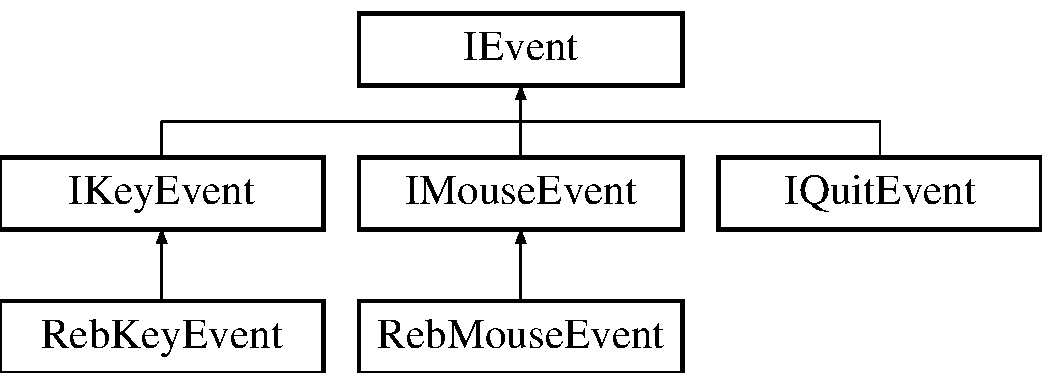
\includegraphics[height=3.000000cm]{class_i_event}
\end{center}
\end{figure}
\subsection*{Public Member Functions}
\begin{DoxyCompactItemize}
\item 
virtual Reb\+Event\+Type {\bfseries Get\+Type} ()=0\hypertarget{class_i_event_acca503dbd25c63119aa0dd4c36e3a148}{}\label{class_i_event_acca503dbd25c63119aa0dd4c36e3a148}

\item 
virtual std\+::string {\bfseries Get\+Add\+Info} ()=0\hypertarget{class_i_event_a9a1417c438733cec89a00f1a97c6cfd9}{}\label{class_i_event_a9a1417c438733cec89a00f1a97c6cfd9}

\end{DoxyCompactItemize}


The documentation for this class was generated from the following file\+:\begin{DoxyCompactItemize}
\item 
Code/\+Rimba/I\+Event.\+h\end{DoxyCompactItemize}

\hypertarget{class_i_event_listener}{}\section{I\+Event\+Listener Class Reference}
\label{class_i_event_listener}\index{I\+Event\+Listener@{I\+Event\+Listener}}
Inheritance diagram for I\+Event\+Listener\+:\begin{figure}[H]
\begin{center}
\leavevmode
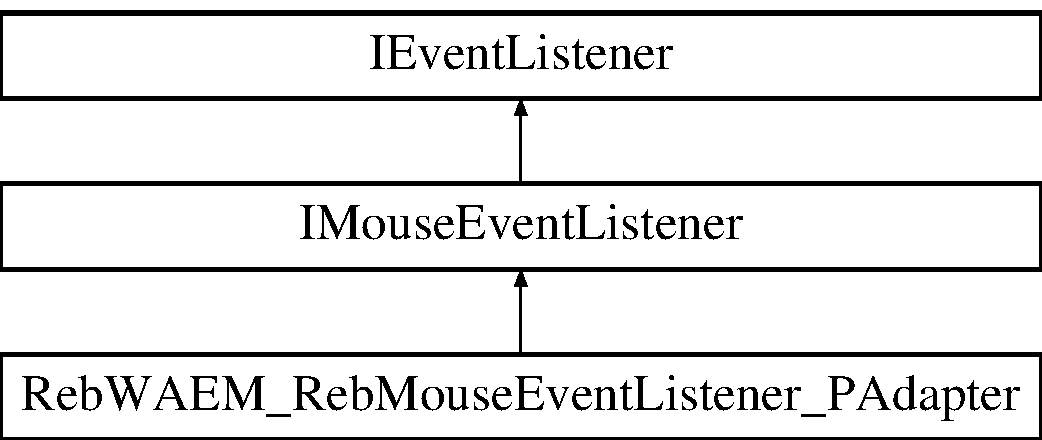
\includegraphics[height=3.000000cm]{class_i_event_listener}
\end{center}
\end{figure}
\subsection*{Public Member Functions}
\begin{DoxyCompactItemize}
\item 
virtual void {\bfseries on\+Event} (\hyperlink{class_i_event}{I\+Event} $\ast$ev)=0\hypertarget{class_i_event_listener_a967fcdde8dbc56c39c51b5280f1e4d3b}{}\label{class_i_event_listener_a967fcdde8dbc56c39c51b5280f1e4d3b}

\end{DoxyCompactItemize}


The documentation for this class was generated from the following file\+:\begin{DoxyCompactItemize}
\item 
Code/\+Rimba/I\+Event.\+h\end{DoxyCompactItemize}

\hypertarget{class_i_game}{}\section{I\+Game Class Reference}
\label{class_i_game}\index{I\+Game@{I\+Game}}
Inheritance diagram for I\+Game\+:\begin{figure}[H]
\begin{center}
\leavevmode
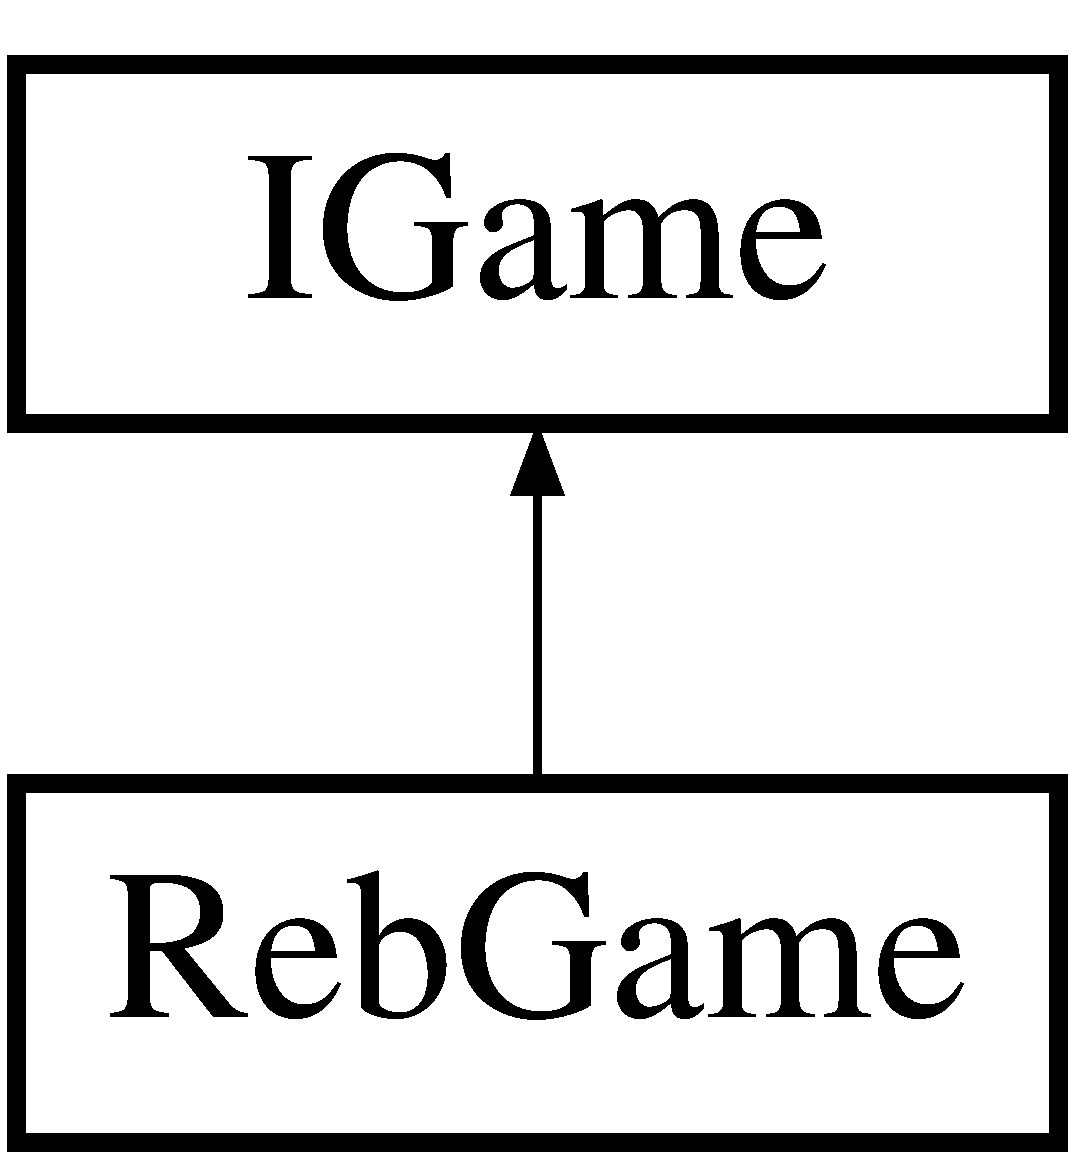
\includegraphics[height=2.000000cm]{class_i_game}
\end{center}
\end{figure}
\subsection*{Public Member Functions}
\begin{DoxyCompactItemize}
\item 
virtual void {\bfseries Init} ()=0\hypertarget{class_i_game_a870431190d7ddb5dbde09cfb0eb6b586}{}\label{class_i_game_a870431190d7ddb5dbde09cfb0eb6b586}

\item 
virtual void {\bfseries Game\+Loop} ()=0\hypertarget{class_i_game_ad57c83ac50795783d3b774594df6752b}{}\label{class_i_game_ad57c83ac50795783d3b774594df6752b}

\item 
virtual void {\bfseries Release} ()=0\hypertarget{class_i_game_afa3c24e8569f8ab61289c10c101a7fd9}{}\label{class_i_game_afa3c24e8569f8ab61289c10c101a7fd9}

\end{DoxyCompactItemize}


The documentation for this class was generated from the following file\+:\begin{DoxyCompactItemize}
\item 
Code/\+Rimba/I\+Game.\+h\end{DoxyCompactItemize}

\hypertarget{class_i_game_env}{}\section{I\+Game\+Env Class Reference}
\label{class_i_game_env}\index{I\+Game\+Env@{I\+Game\+Env}}
Inheritance diagram for I\+Game\+Env\+:\begin{figure}[H]
\begin{center}
\leavevmode
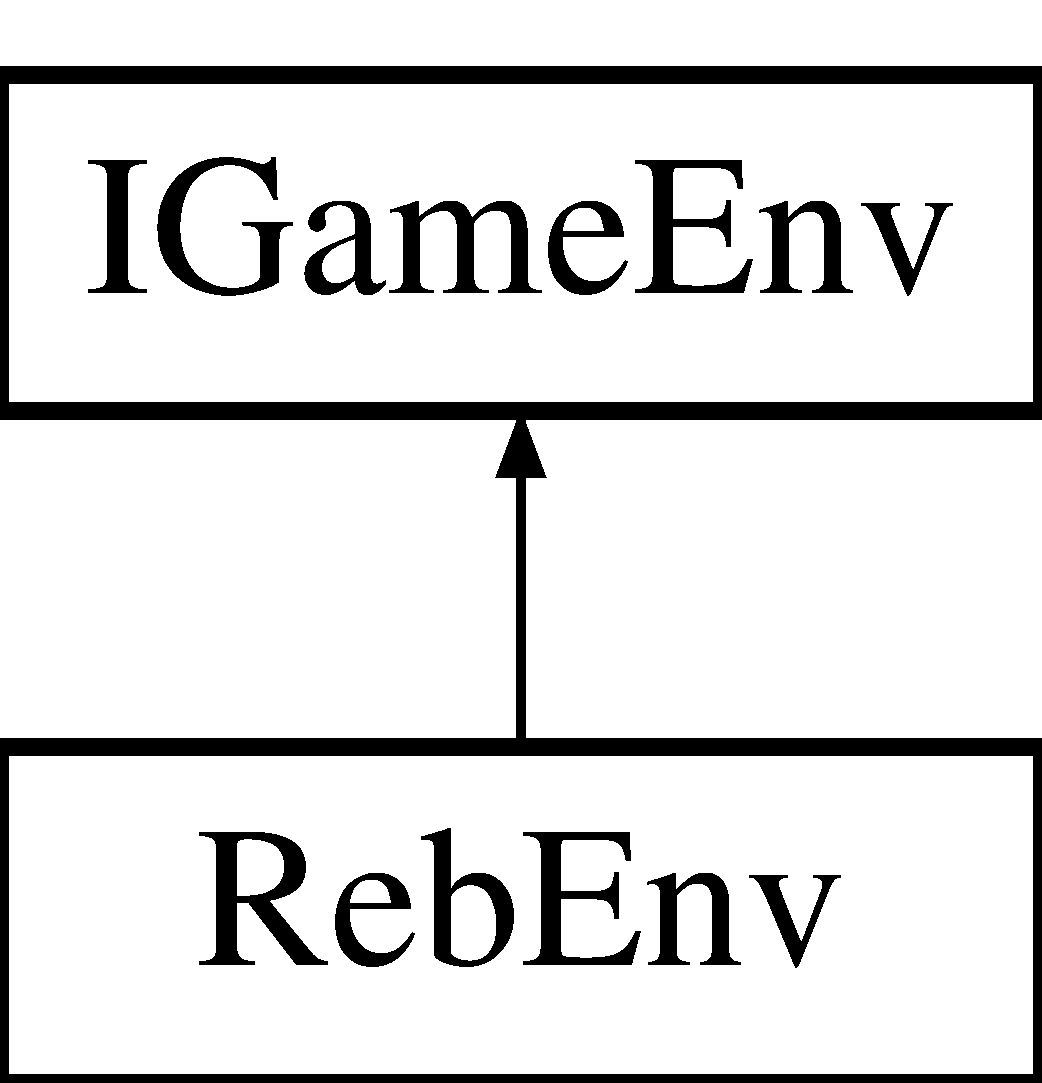
\includegraphics[height=2.000000cm]{class_i_game_env}
\end{center}
\end{figure}
\subsection*{Public Member Functions}
\begin{DoxyCompactItemize}
\item 
virtual \hyperlink{class_i_terrain}{I\+Terrain} $\ast$ {\bfseries Create\+Terrain} ()=0\hypertarget{class_i_game_env_a0e14b7622d8a2707e6eecb86699f97ce}{}\label{class_i_game_env_a0e14b7622d8a2707e6eecb86699f97ce}

\item 
virtual \hyperlink{class_i_terrain}{I\+Terrain} $\ast$ {\bfseries Create\+Terrain} (std\+::string frp)=0\hypertarget{class_i_game_env_af375523ae99a795ef4889e47861ce391}{}\label{class_i_game_env_af375523ae99a795ef4889e47861ce391}

\item 
virtual std\+::vector$<$ \hyperlink{class_i_terrain}{I\+Terrain} $\ast$ $>$ $\ast$ {\bfseries Get\+Terrains} ()=0\hypertarget{class_i_game_env_ab917525b0b0b751924b26a98825f1681}{}\label{class_i_game_env_ab917525b0b0b751924b26a98825f1681}

\item 
virtual void {\bfseries Delete\+Terrain} (\hyperlink{class_i_terrain}{I\+Terrain} $\ast$del)=0\hypertarget{class_i_game_env_a4ef200439b989df4463c00a19064be00}{}\label{class_i_game_env_a4ef200439b989df4463c00a19064be00}

\end{DoxyCompactItemize}


The documentation for this class was generated from the following file\+:\begin{DoxyCompactItemize}
\item 
Code/\+Rimba/I\+Render\+Device.\+h\end{DoxyCompactItemize}

\hypertarget{class_i_game_logic}{}\section{I\+Game\+Logic Class Reference}
\label{class_i_game_logic}\index{I\+Game\+Logic@{I\+Game\+Logic}}
Inheritance diagram for I\+Game\+Logic\+:\begin{figure}[H]
\begin{center}
\leavevmode
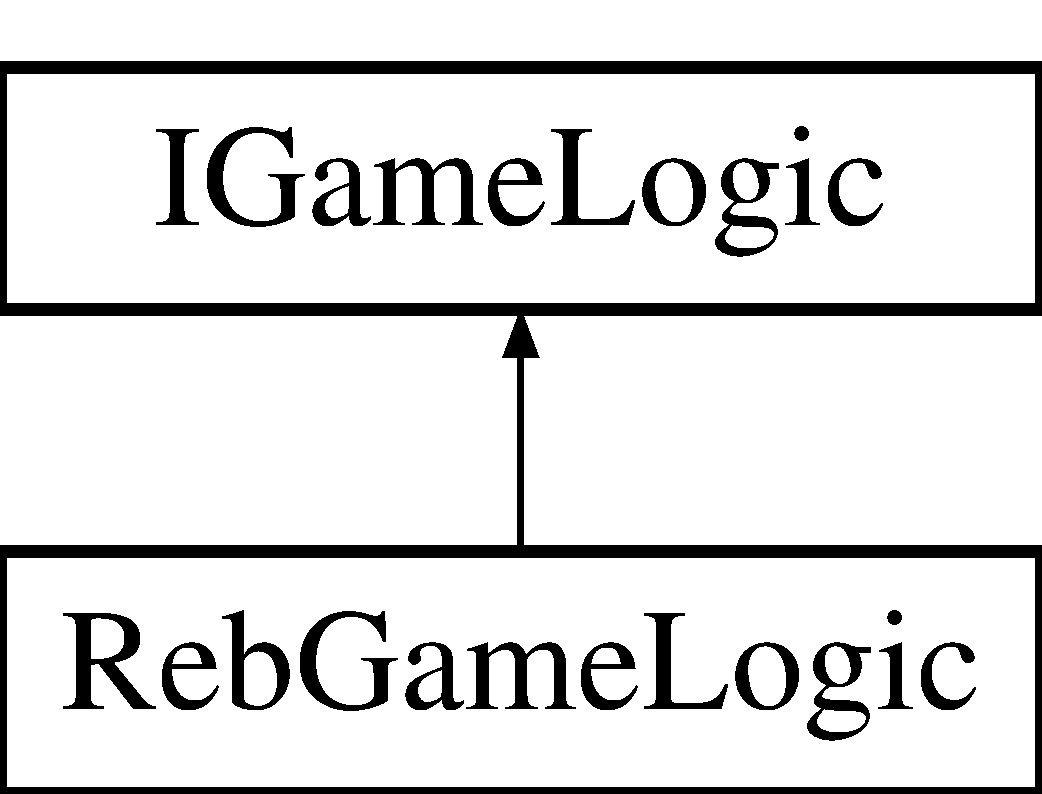
\includegraphics[height=2.000000cm]{class_i_game_logic}
\end{center}
\end{figure}


The documentation for this class was generated from the following file\+:\begin{DoxyCompactItemize}
\item 
Code/\+Rimba/I\+Game\+Logic.\+h\end{DoxyCompactItemize}

\hypertarget{class_i_image_handler}{}\section{I\+Image\+Handler Class Reference}
\label{class_i_image_handler}\index{I\+Image\+Handler@{I\+Image\+Handler}}
Inheritance diagram for I\+Image\+Handler\+:\begin{figure}[H]
\begin{center}
\leavevmode
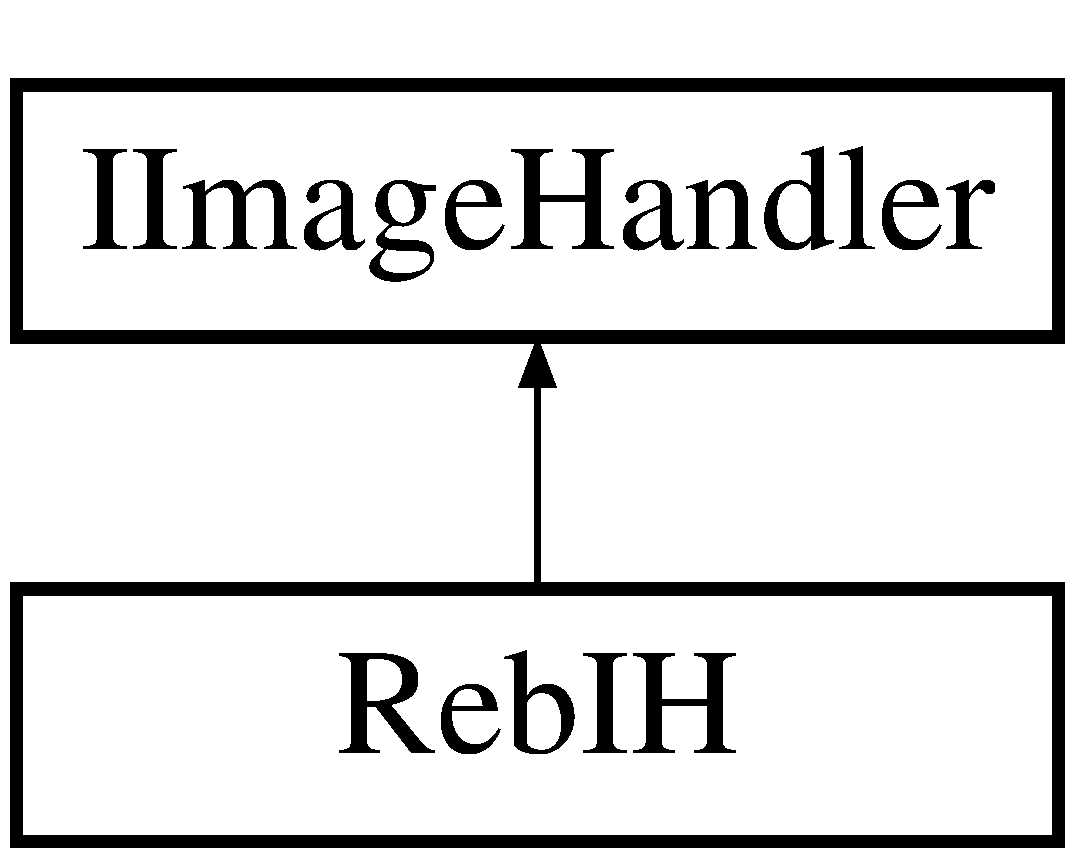
\includegraphics[height=2.000000cm]{class_i_image_handler}
\end{center}
\end{figure}
\subsection*{Public Member Functions}
\begin{DoxyCompactItemize}
\item 
virtual void {\bfseries Load\+File} (std\+::string file)=0\hypertarget{class_i_image_handler_a823b11871d4fcc40e8e18a94820d0b4f}{}\label{class_i_image_handler_a823b11871d4fcc40e8e18a94820d0b4f}

\item 
virtual unsigned int {\bfseries Get\+Width} ()=0\hypertarget{class_i_image_handler_a662c52ad92e02fe21a7d55988cbaa25b}{}\label{class_i_image_handler_a662c52ad92e02fe21a7d55988cbaa25b}

\item 
virtual unsigned int {\bfseries Get\+Height} ()=0\hypertarget{class_i_image_handler_aaaee578873610c53daf1222b583fd0c1}{}\label{class_i_image_handler_aaaee578873610c53daf1222b583fd0c1}

\item 
virtual Reb\+Vector {\bfseries Get\+Pixel\+Color} (unsigned int x, unsigned int y)=0\hypertarget{class_i_image_handler_abc699356ff81d184e3094685d819cb74}{}\label{class_i_image_handler_abc699356ff81d184e3094685d819cb74}

\item 
virtual void {\bfseries Load\+Into\+Renderer} ()=0\hypertarget{class_i_image_handler_a88de4b52867448c3928e1a2c461e5e15}{}\label{class_i_image_handler_a88de4b52867448c3928e1a2c461e5e15}

\end{DoxyCompactItemize}


The documentation for this class was generated from the following file\+:\begin{DoxyCompactItemize}
\item 
Code/\+Rimba/I\+Render\+Device.\+h\end{DoxyCompactItemize}

\hypertarget{class_i_key_event}{}\section{I\+Key\+Event Class Reference}
\label{class_i_key_event}\index{I\+Key\+Event@{I\+Key\+Event}}
Inheritance diagram for I\+Key\+Event\+:\begin{figure}[H]
\begin{center}
\leavevmode
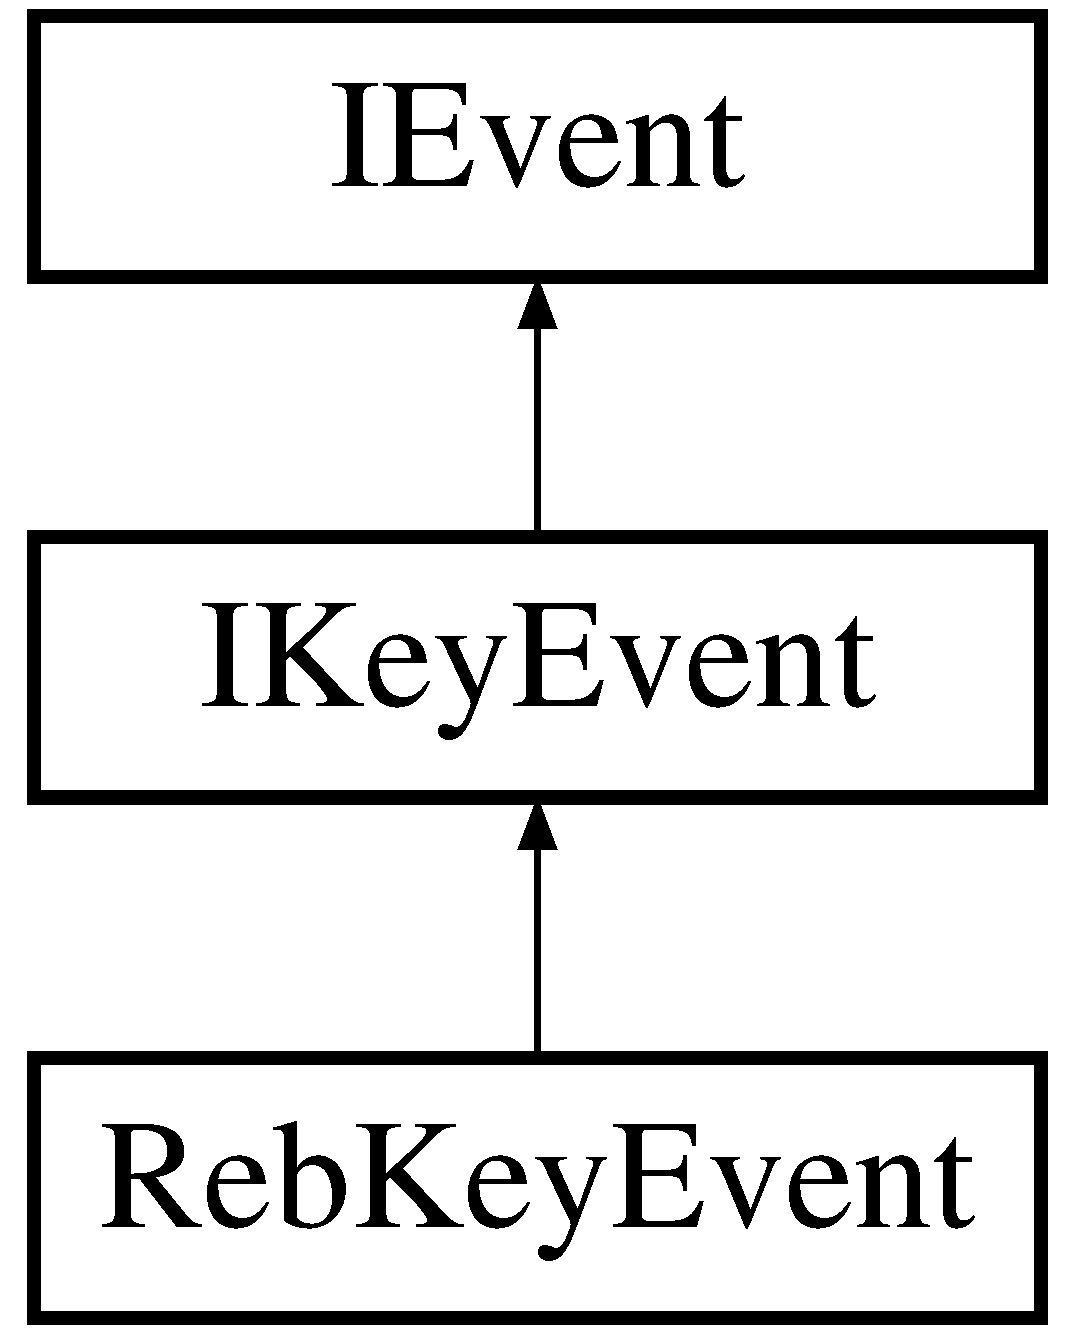
\includegraphics[height=3.000000cm]{class_i_key_event}
\end{center}
\end{figure}
\subsection*{Public Member Functions}
\begin{DoxyCompactItemize}
\item 
virtual Reb\+Key\+Code {\bfseries Get\+Key} ()=0\hypertarget{class_i_key_event_ac1bb509d634d0becb89d48978a13a4bf}{}\label{class_i_key_event_ac1bb509d634d0becb89d48978a13a4bf}

\item 
virtual bool {\bfseries P\+OR} ()=0\hypertarget{class_i_key_event_a79250362b1d20b15bb7768449d9eae58}{}\label{class_i_key_event_a79250362b1d20b15bb7768449d9eae58}

\end{DoxyCompactItemize}


The documentation for this class was generated from the following file\+:\begin{DoxyCompactItemize}
\item 
Code/\+Rimba/I\+Event.\+h\end{DoxyCompactItemize}

\hypertarget{class_i_key_listener}{}\section{I\+Key\+Listener Class Reference}
\label{class_i_key_listener}\index{I\+Key\+Listener@{I\+Key\+Listener}}
Inheritance diagram for I\+Key\+Listener\+:\begin{figure}[H]
\begin{center}
\leavevmode
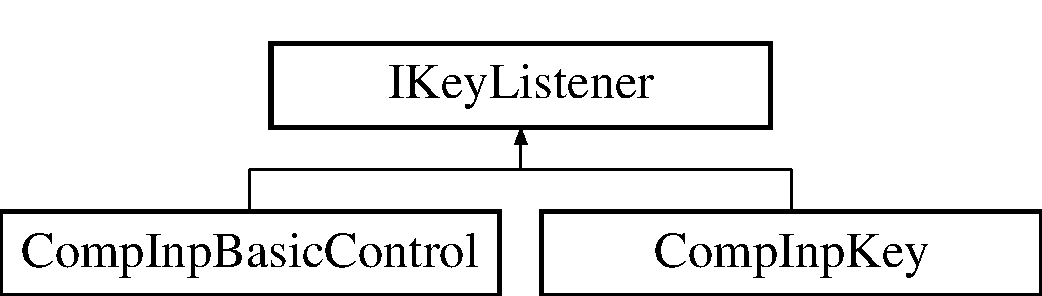
\includegraphics[height=2.000000cm]{class_i_key_listener}
\end{center}
\end{figure}
\subsection*{Public Member Functions}
\begin{DoxyCompactItemize}
\item 
virtual void {\bfseries on\+Key\+Event} (\hyperlink{union_reb_event}{Reb\+Event} keyev)\hypertarget{class_i_key_listener_a53153f0f68d614e3524a3a3dd2f48f95}{}\label{class_i_key_listener_a53153f0f68d614e3524a3a3dd2f48f95}

\end{DoxyCompactItemize}


The documentation for this class was generated from the following file\+:\begin{DoxyCompactItemize}
\item 
Code/\+Reb\+Window/Event\+Listeners.\+h\end{DoxyCompactItemize}

\hypertarget{class_i_light}{}\section{I\+Light Class Reference}
\label{class_i_light}\index{I\+Light@{I\+Light}}
Inheritance diagram for I\+Light\+:\begin{figure}[H]
\begin{center}
\leavevmode
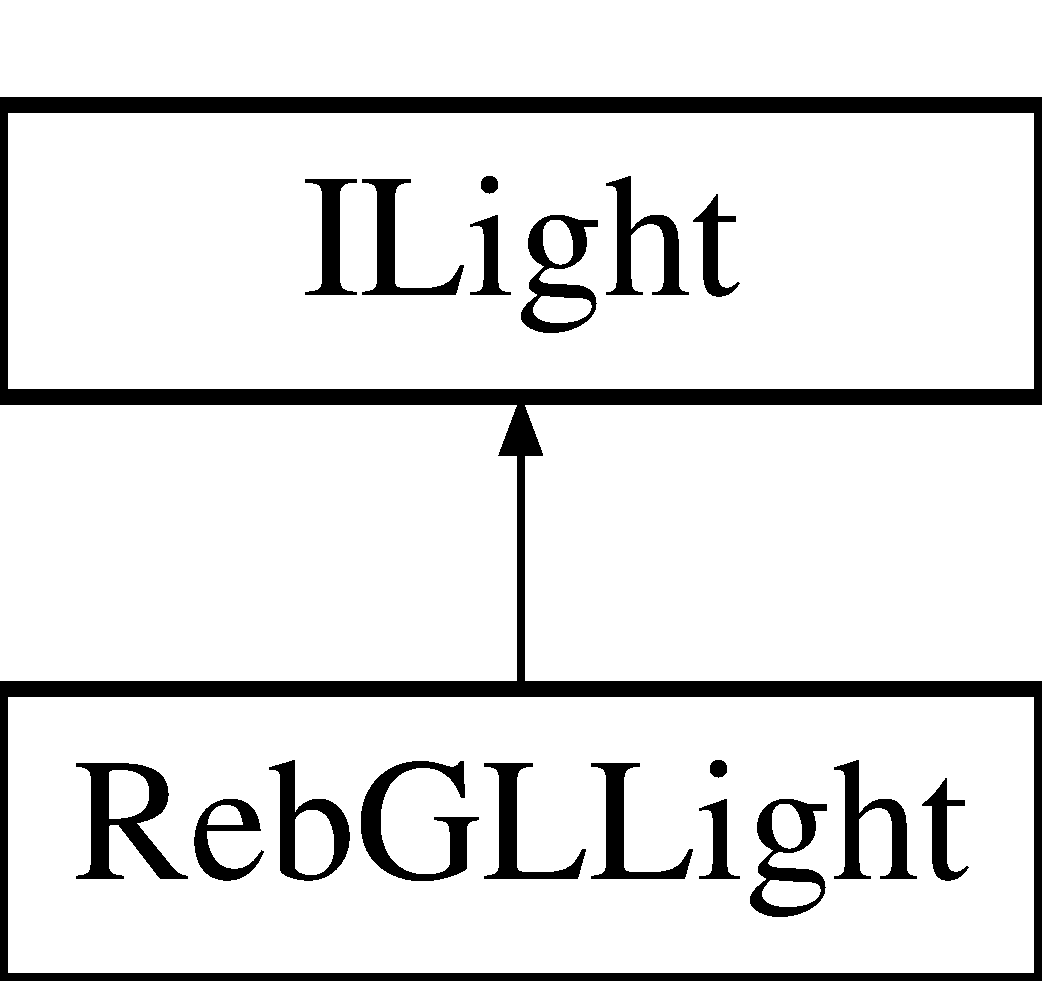
\includegraphics[height=2.000000cm]{class_i_light}
\end{center}
\end{figure}
\subsection*{Public Member Functions}
\begin{DoxyCompactItemize}
\item 
virtual Reb\+Vector {\bfseries Get\+Pos} ()=0\hypertarget{class_i_light_aab76acc774f2851d11973376d0ab72b3}{}\label{class_i_light_aab76acc774f2851d11973376d0ab72b3}

\item 
virtual Reb\+Vector {\bfseries Get\+Color} ()=0\hypertarget{class_i_light_a1e4c3950728932cfd29eb94da766a2f1}{}\label{class_i_light_a1e4c3950728932cfd29eb94da766a2f1}

\end{DoxyCompactItemize}


The documentation for this class was generated from the following file\+:\begin{DoxyCompactItemize}
\item 
Code/\+Rimba/Reb\+Graphic\+Elements.\+h\end{DoxyCompactItemize}

\hypertarget{class_i_light_system}{}\section{I\+Light\+System Class Reference}
\label{class_i_light_system}\index{I\+Light\+System@{I\+Light\+System}}
Inheritance diagram for I\+Light\+System\+:\begin{figure}[H]
\begin{center}
\leavevmode
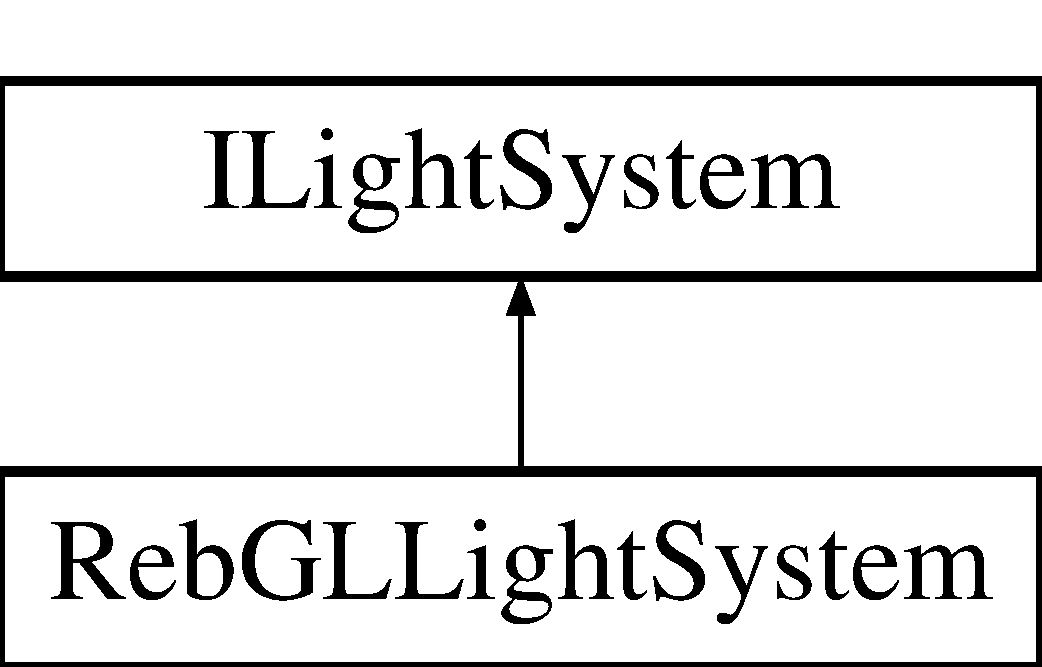
\includegraphics[height=2.000000cm]{class_i_light_system}
\end{center}
\end{figure}


The documentation for this class was generated from the following file\+:\begin{DoxyCompactItemize}
\item 
Code/\+Rimba/I\+Render\+Device.\+h\end{DoxyCompactItemize}

\hypertarget{class_i_material}{}\section{I\+Material Class Reference}
\label{class_i_material}\index{I\+Material@{I\+Material}}
Inheritance diagram for I\+Material\+:\begin{figure}[H]
\begin{center}
\leavevmode
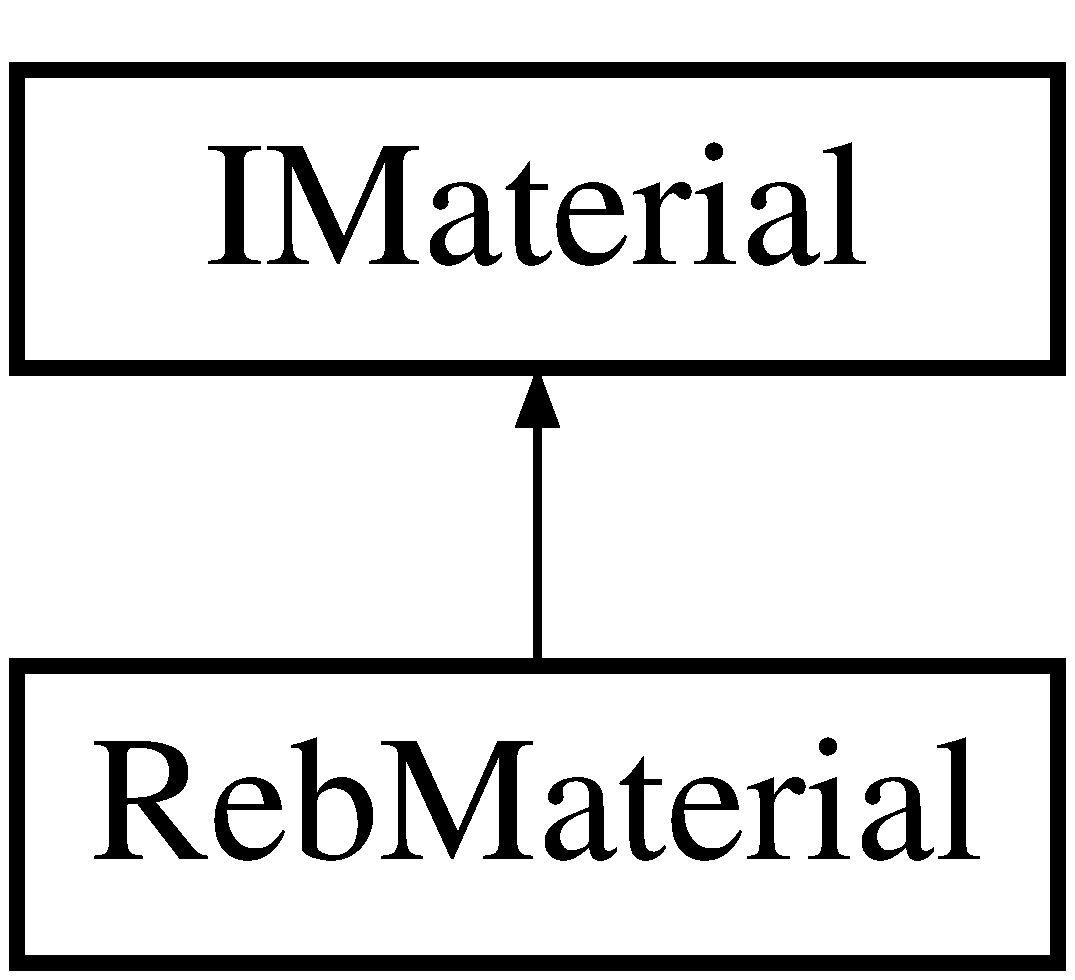
\includegraphics[height=2.000000cm]{class_i_material}
\end{center}
\end{figure}
\subsection*{Public Member Functions}
\begin{DoxyCompactItemize}
\item 
virtual void {\bfseries Bind} ()=0\hypertarget{class_i_material_a0bf1f5681d82e5e8fb0a393cdff4fab5}{}\label{class_i_material_a0bf1f5681d82e5e8fb0a393cdff4fab5}

\end{DoxyCompactItemize}


The documentation for this class was generated from the following file\+:\begin{DoxyCompactItemize}
\item 
Code/\+Rimba/Reb\+Graphic\+Elements.\+h\end{DoxyCompactItemize}

\hypertarget{class_i_m_e_h}{}\section{I\+M\+EH Class Reference}
\label{class_i_m_e_h}\index{I\+M\+EH@{I\+M\+EH}}
Inheritance diagram for I\+M\+EH\+:\begin{figure}[H]
\begin{center}
\leavevmode
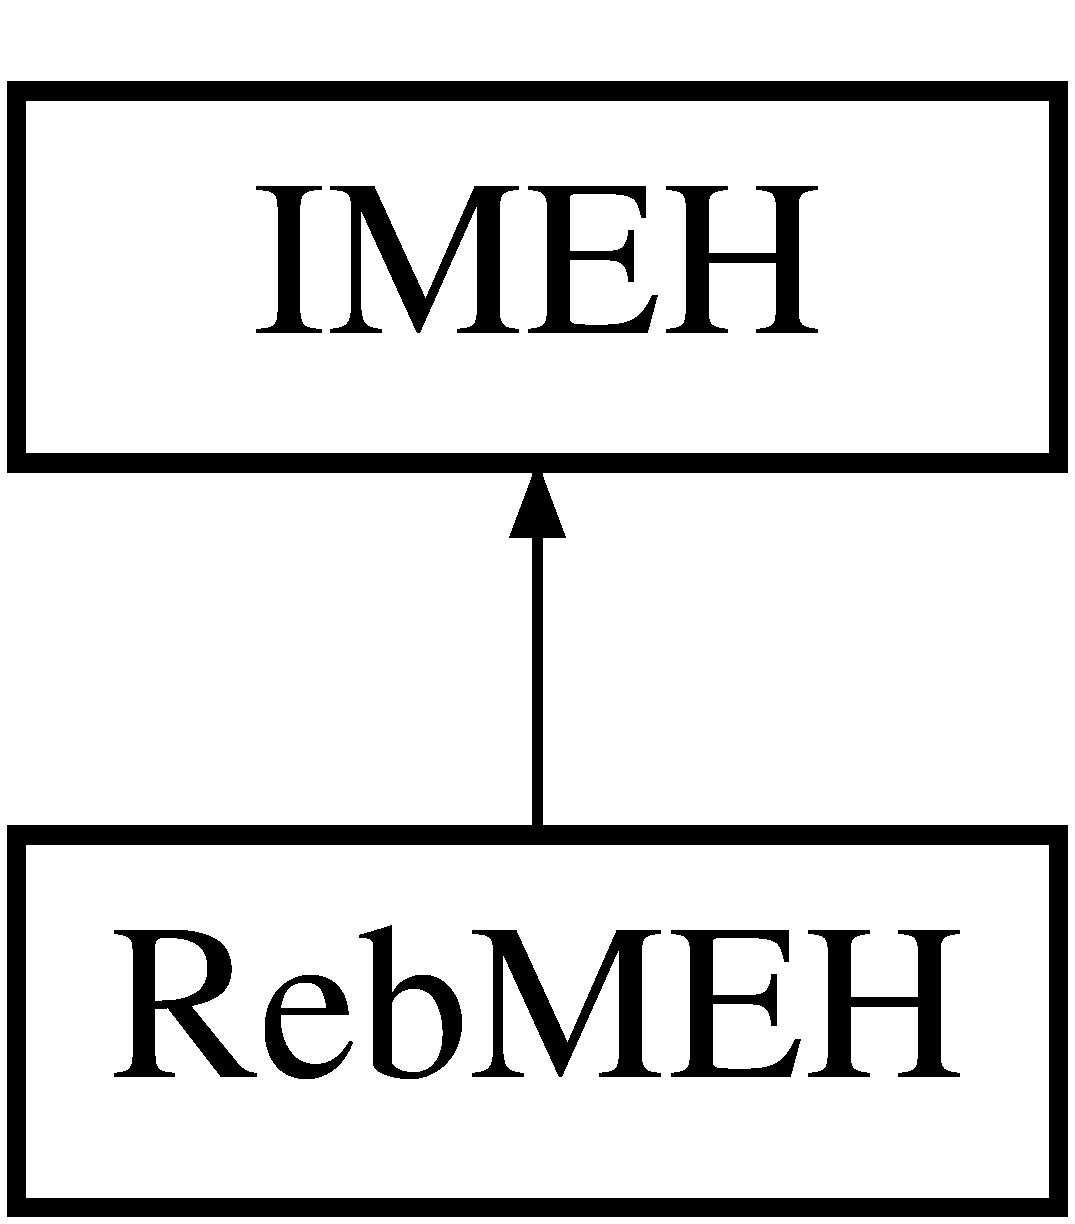
\includegraphics[height=2.000000cm]{class_i_m_e_h}
\end{center}
\end{figure}
\subsection*{Public Member Functions}
\begin{DoxyCompactItemize}
\item 
virtual void {\bfseries Init} (\hyperlink{class_reb_g_d_c}{Reb\+G\+DC} $\ast$data)=0\hypertarget{class_i_m_e_h_a808b102bf9f8281aef8b4cb17652613c}{}\label{class_i_m_e_h_a808b102bf9f8281aef8b4cb17652613c}

\item 
virtual void {\bfseries Release} ()=0\hypertarget{class_i_m_e_h_ac47c3471945c993f1b4dfb35d8dd4a23}{}\label{class_i_m_e_h_ac47c3471945c993f1b4dfb35d8dd4a23}

\item 
virtual void {\bfseries Add\+Event} (\hyperlink{union_reb_event}{Reb\+Event} Event)=0\hypertarget{class_i_m_e_h_aa12fb49a27156061fe02c56b928963e5}{}\label{class_i_m_e_h_aa12fb49a27156061fe02c56b928963e5}

\item 
virtual void {\bfseries Translate\+Event} (\hyperlink{union_reb_event}{Reb\+Event} $\ast$Event)=0\hypertarget{class_i_m_e_h_aeb04da4f2405b896c93d299d0e17aa4c}{}\label{class_i_m_e_h_aeb04da4f2405b896c93d299d0e17aa4c}

\item 
virtual void {\bfseries Register\+Key\+Event\+Listener} (\hyperlink{class_i_key_listener}{I\+Key\+Listener} $\ast$ikl)=0\hypertarget{class_i_m_e_h_ae5c0421dd64b696ef51227254d18efe6}{}\label{class_i_m_e_h_ae5c0421dd64b696ef51227254d18efe6}

\item 
virtual void {\bfseries Un\+Register\+Key\+Event\+Listener} (\hyperlink{class_i_key_listener}{I\+Key\+Listener} $\ast$ikl)=0\hypertarget{class_i_m_e_h_a08078182c8d0b334e941a4314719fa68}{}\label{class_i_m_e_h_a08078182c8d0b334e941a4314719fa68}

\item 
virtual void {\bfseries Register\+Mouse\+Event\+Listener} (\hyperlink{class_i_mouse_listener}{I\+Mouse\+Listener} $\ast$iml)=0\hypertarget{class_i_m_e_h_a06ad1a6f9111d62e428c4047575323b2}{}\label{class_i_m_e_h_a06ad1a6f9111d62e428c4047575323b2}

\item 
virtual void {\bfseries Un\+Register\+Mouse\+Event\+Listener} (\hyperlink{class_i_mouse_listener}{I\+Mouse\+Listener} $\ast$iml)=0\hypertarget{class_i_m_e_h_a5f0ca9fd2c0e154eb7760b64ab2953a7}{}\label{class_i_m_e_h_a5f0ca9fd2c0e154eb7760b64ab2953a7}

\item 
virtual void {\bfseries Init} (\hyperlink{class_reb_g_d_c}{Reb\+G\+DC} $\ast$data)=0\hypertarget{class_i_m_e_h_a808b102bf9f8281aef8b4cb17652613c}{}\label{class_i_m_e_h_a808b102bf9f8281aef8b4cb17652613c}

\item 
virtual void {\bfseries Release} ()=0\hypertarget{class_i_m_e_h_ac47c3471945c993f1b4dfb35d8dd4a23}{}\label{class_i_m_e_h_ac47c3471945c993f1b4dfb35d8dd4a23}

\item 
virtual void {\bfseries Add\+Event} (\hyperlink{union_reb_event}{Reb\+Event} Event)=0\hypertarget{class_i_m_e_h_aa12fb49a27156061fe02c56b928963e5}{}\label{class_i_m_e_h_aa12fb49a27156061fe02c56b928963e5}

\item 
virtual void {\bfseries Translate\+Event} (\hyperlink{union_reb_event}{Reb\+Event} $\ast$Event)=0\hypertarget{class_i_m_e_h_aeb04da4f2405b896c93d299d0e17aa4c}{}\label{class_i_m_e_h_aeb04da4f2405b896c93d299d0e17aa4c}

\item 
virtual void {\bfseries Register\+Key\+Event\+Listener} (\hyperlink{class_i_key_listener}{I\+Key\+Listener} $\ast$ikl)=0\hypertarget{class_i_m_e_h_ae5c0421dd64b696ef51227254d18efe6}{}\label{class_i_m_e_h_ae5c0421dd64b696ef51227254d18efe6}

\item 
virtual void {\bfseries Un\+Register\+Key\+Event\+Listener} (\hyperlink{class_i_key_listener}{I\+Key\+Listener} $\ast$ikl)=0\hypertarget{class_i_m_e_h_a08078182c8d0b334e941a4314719fa68}{}\label{class_i_m_e_h_a08078182c8d0b334e941a4314719fa68}

\item 
virtual void {\bfseries Register\+Mouse\+Event\+Listener} (\hyperlink{class_i_mouse_listener}{I\+Mouse\+Listener} $\ast$iml)=0\hypertarget{class_i_m_e_h_a06ad1a6f9111d62e428c4047575323b2}{}\label{class_i_m_e_h_a06ad1a6f9111d62e428c4047575323b2}

\item 
virtual void {\bfseries Un\+Register\+Mouse\+Event\+Listener} (\hyperlink{class_i_mouse_listener}{I\+Mouse\+Listener} $\ast$iml)=0\hypertarget{class_i_m_e_h_a5f0ca9fd2c0e154eb7760b64ab2953a7}{}\label{class_i_m_e_h_a5f0ca9fd2c0e154eb7760b64ab2953a7}

\end{DoxyCompactItemize}


The documentation for this class was generated from the following file\+:\begin{DoxyCompactItemize}
\item 
Code/\+Reb\+Window/I\+M\+E\+H.\+h\end{DoxyCompactItemize}

\hypertarget{class_i_model_handler}{}\section{I\+Model\+Handler Class Reference}
\label{class_i_model_handler}\index{I\+Model\+Handler@{I\+Model\+Handler}}
\subsection*{Public Member Functions}
\begin{DoxyCompactItemize}
\item 
virtual bool {\bfseries Load\+Model} (std\+::string file)=0\hypertarget{class_i_model_handler_a856b580323561f2dbb795b9fbdf423a4}{}\label{class_i_model_handler_a856b580323561f2dbb795b9fbdf423a4}

\item 
virtual \hyperlink{class_i_vertex_cache}{I\+Vertex\+Cache} $\ast$ {\bfseries Get\+R\+VC} ()=0\hypertarget{class_i_model_handler_a5841a6203a14ec351528583229320ec7}{}\label{class_i_model_handler_a5841a6203a14ec351528583229320ec7}

\end{DoxyCompactItemize}


The documentation for this class was generated from the following file\+:\begin{DoxyCompactItemize}
\item 
Code/\+Rimba/I\+Render\+Device.\+h\end{DoxyCompactItemize}

\hypertarget{class_i_mouse_event}{}\section{I\+Mouse\+Event Class Reference}
\label{class_i_mouse_event}\index{I\+Mouse\+Event@{I\+Mouse\+Event}}
Inheritance diagram for I\+Mouse\+Event\+:\begin{figure}[H]
\begin{center}
\leavevmode
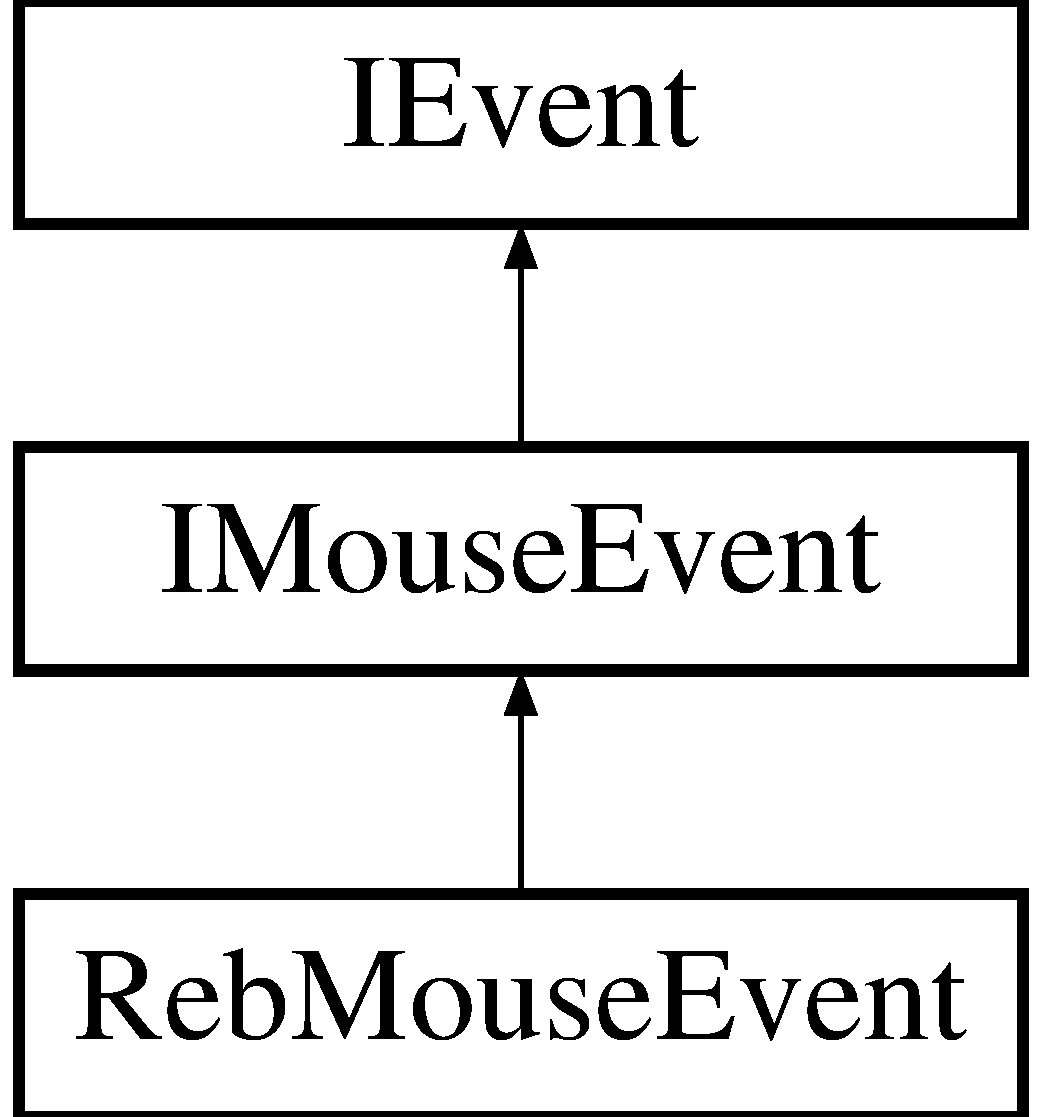
\includegraphics[height=3.000000cm]{class_i_mouse_event}
\end{center}
\end{figure}
\subsection*{Public Member Functions}
\begin{DoxyCompactItemize}
\item 
virtual Reb\+Key\+Code {\bfseries Get\+Mouse\+Key} ()=0\hypertarget{class_i_mouse_event_a19eaee1abd03bde73f7dd82485974b37}{}\label{class_i_mouse_event_a19eaee1abd03bde73f7dd82485974b37}

\item 
virtual Reb\+Vector {\bfseries Get\+Pos} ()=0\hypertarget{class_i_mouse_event_aac99d8e620bc14e42423380223ede2c9}{}\label{class_i_mouse_event_aac99d8e620bc14e42423380223ede2c9}

\item 
virtual int {\bfseries Get\+PosX} ()=0\hypertarget{class_i_mouse_event_a7e756004af212d5b328eab2720ae610e}{}\label{class_i_mouse_event_a7e756004af212d5b328eab2720ae610e}

\item 
virtual int {\bfseries Get\+PosY} ()=0\hypertarget{class_i_mouse_event_ac29224c0cbca1989c51775f6690f10ec}{}\label{class_i_mouse_event_ac29224c0cbca1989c51775f6690f10ec}

\item 
virtual int {\bfseries Get\+MoveX} ()=0\hypertarget{class_i_mouse_event_a4f870ca90e0d659ff34f5cf7bba7dacf}{}\label{class_i_mouse_event_a4f870ca90e0d659ff34f5cf7bba7dacf}

\item 
virtual int {\bfseries Get\+MoveY} ()=0\hypertarget{class_i_mouse_event_a4d24e7ee9ce321d2e704d81386f973ea}{}\label{class_i_mouse_event_a4d24e7ee9ce321d2e704d81386f973ea}

\end{DoxyCompactItemize}


The documentation for this class was generated from the following file\+:\begin{DoxyCompactItemize}
\item 
Code/\+Rimba/I\+Event.\+h\end{DoxyCompactItemize}

\hypertarget{class_i_mouse_event_listener}{}\section{I\+Mouse\+Event\+Listener Class Reference}
\label{class_i_mouse_event_listener}\index{I\+Mouse\+Event\+Listener@{I\+Mouse\+Event\+Listener}}
Inheritance diagram for I\+Mouse\+Event\+Listener\+:\begin{figure}[H]
\begin{center}
\leavevmode
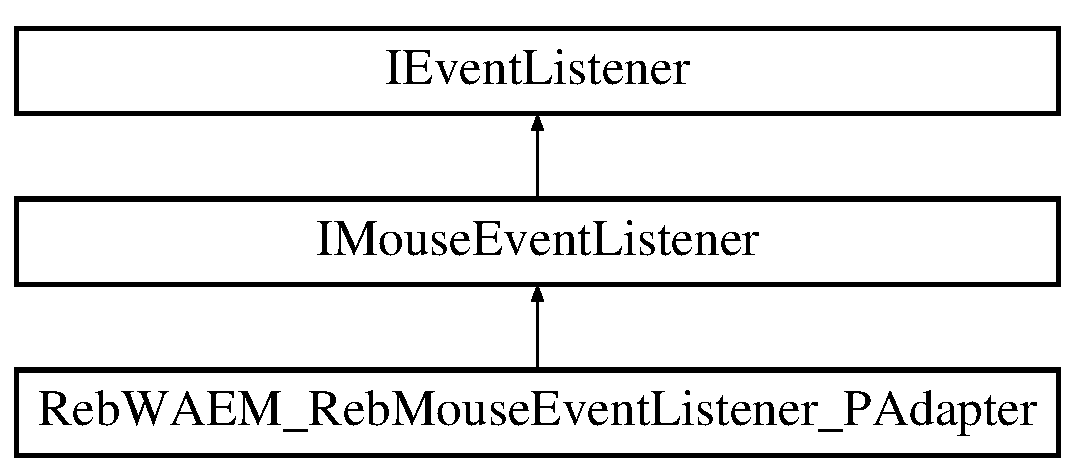
\includegraphics[height=3.000000cm]{class_i_mouse_event_listener}
\end{center}
\end{figure}
\subsection*{Public Member Functions}
\begin{DoxyCompactItemize}
\item 
virtual void {\bfseries on\+Move} (\hyperlink{class_i_mouse_event}{I\+Mouse\+Event} $\ast$me)=0\hypertarget{class_i_mouse_event_listener_a2fd54983aa8a932e93c792425641c5d1}{}\label{class_i_mouse_event_listener_a2fd54983aa8a932e93c792425641c5d1}

\item 
virtual void {\bfseries on\+Key\+Press} (\hyperlink{class_i_mouse_event}{I\+Mouse\+Event} $\ast$me)=0\hypertarget{class_i_mouse_event_listener_a2ef49eea9335b7fae7fb8fbc3f730e8c}{}\label{class_i_mouse_event_listener_a2ef49eea9335b7fae7fb8fbc3f730e8c}

\end{DoxyCompactItemize}


The documentation for this class was generated from the following file\+:\begin{DoxyCompactItemize}
\item 
Code/\+Rimba/I\+Event.\+h\end{DoxyCompactItemize}

\hypertarget{class_i_mouse_listener}{}\section{I\+Mouse\+Listener Class Reference}
\label{class_i_mouse_listener}\index{I\+Mouse\+Listener@{I\+Mouse\+Listener}}
Inheritance diagram for I\+Mouse\+Listener\+:\begin{figure}[H]
\begin{center}
\leavevmode
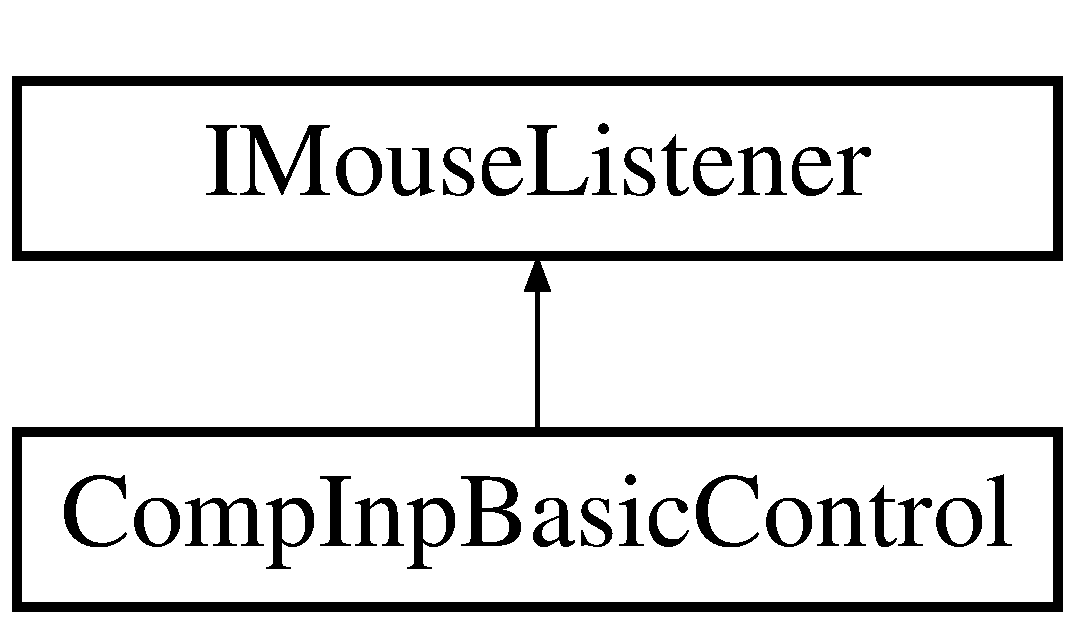
\includegraphics[height=2.000000cm]{class_i_mouse_listener}
\end{center}
\end{figure}
\subsection*{Public Member Functions}
\begin{DoxyCompactItemize}
\item 
virtual void {\bfseries on\+M\+Key\+Event} (\hyperlink{union_reb_event}{Reb\+Event} mev)\hypertarget{class_i_mouse_listener_af770f498d374d8e63e97039ab4177253}{}\label{class_i_mouse_listener_af770f498d374d8e63e97039ab4177253}

\item 
virtual void {\bfseries on\+M\+Motion\+Event} (\hyperlink{union_reb_event}{Reb\+Event} mev)\hypertarget{class_i_mouse_listener_aa862db142bafd7ed53ce2ebdceefef00}{}\label{class_i_mouse_listener_aa862db142bafd7ed53ce2ebdceefef00}

\end{DoxyCompactItemize}


The documentation for this class was generated from the following file\+:\begin{DoxyCompactItemize}
\item 
Code/\+Reb\+Window/Event\+Listeners.\+h\end{DoxyCompactItemize}

\hypertarget{class_i_music_player}{}\section{I\+Music\+Player Class Reference}
\label{class_i_music_player}\index{I\+Music\+Player@{I\+Music\+Player}}
\subsection*{Public Member Functions}
\begin{DoxyCompactItemize}
\item 
virtual void {\bfseries Init} ()=0\hypertarget{class_i_music_player_a695e6d7ff2dcb18519ef62802cfd20a8}{}\label{class_i_music_player_a695e6d7ff2dcb18519ef62802cfd20a8}

\item 
virtual void {\bfseries Release} ()=0\hypertarget{class_i_music_player_a83f80991f61467a1bb9e7638a91132b3}{}\label{class_i_music_player_a83f80991f61467a1bb9e7638a91132b3}

\item 
virtual void {\bfseries Play} ()=0\hypertarget{class_i_music_player_a2bb20e18b2124e3466bc483addafc8ad}{}\label{class_i_music_player_a2bb20e18b2124e3466bc483addafc8ad}

\item 
virtual bool {\bfseries Set\+Source} (std\+::string file)=0\hypertarget{class_i_music_player_a4fb663480af59b9583635d8889af3f6e}{}\label{class_i_music_player_a4fb663480af59b9583635d8889af3f6e}

\item 
virtual bool {\bfseries Set\+Source} (U\+I\+NT ID)=0\hypertarget{class_i_music_player_af0b438570293b67772c83bf2d86f13b5}{}\label{class_i_music_player_af0b438570293b67772c83bf2d86f13b5}

\item 
virtual void {\bfseries Pause} ()=0\hypertarget{class_i_music_player_a43ca2033b85046541315c3387f3c58eb}{}\label{class_i_music_player_a43ca2033b85046541315c3387f3c58eb}

\item 
virtual void {\bfseries Stop} ()=0\hypertarget{class_i_music_player_ac947647ce3097ca49257cd099852b964}{}\label{class_i_music_player_ac947647ce3097ca49257cd099852b964}

\item 
virtual void {\bfseries Set\+Volume} (float volume)=0\hypertarget{class_i_music_player_aed424daf271bb9d6675fc8c80357d964}{}\label{class_i_music_player_aed424daf271bb9d6675fc8c80357d964}

\item 
virtual bool {\bfseries Is\+Playing} ()=0\hypertarget{class_i_music_player_a6fbae6f26758c70db531cb3a4312c703}{}\label{class_i_music_player_a6fbae6f26758c70db531cb3a4312c703}

\item 
virtual void {\bfseries Init} ()=0\hypertarget{class_i_music_player_a695e6d7ff2dcb18519ef62802cfd20a8}{}\label{class_i_music_player_a695e6d7ff2dcb18519ef62802cfd20a8}

\item 
virtual void {\bfseries Release} ()=0\hypertarget{class_i_music_player_a83f80991f61467a1bb9e7638a91132b3}{}\label{class_i_music_player_a83f80991f61467a1bb9e7638a91132b3}

\item 
virtual void {\bfseries Play} ()=0\hypertarget{class_i_music_player_a2bb20e18b2124e3466bc483addafc8ad}{}\label{class_i_music_player_a2bb20e18b2124e3466bc483addafc8ad}

\item 
virtual bool {\bfseries Set\+Source} (std\+::string file)=0\hypertarget{class_i_music_player_a4fb663480af59b9583635d8889af3f6e}{}\label{class_i_music_player_a4fb663480af59b9583635d8889af3f6e}

\item 
virtual bool {\bfseries Set\+Source} (U\+I\+NT ID)=0\hypertarget{class_i_music_player_af0b438570293b67772c83bf2d86f13b5}{}\label{class_i_music_player_af0b438570293b67772c83bf2d86f13b5}

\item 
virtual void {\bfseries Pause} ()=0\hypertarget{class_i_music_player_a43ca2033b85046541315c3387f3c58eb}{}\label{class_i_music_player_a43ca2033b85046541315c3387f3c58eb}

\item 
virtual void {\bfseries Stop} ()=0\hypertarget{class_i_music_player_ac947647ce3097ca49257cd099852b964}{}\label{class_i_music_player_ac947647ce3097ca49257cd099852b964}

\item 
virtual void {\bfseries Set\+Volume} (float volume)=0\hypertarget{class_i_music_player_aed424daf271bb9d6675fc8c80357d964}{}\label{class_i_music_player_aed424daf271bb9d6675fc8c80357d964}

\item 
virtual bool {\bfseries Is\+Playing} ()=0\hypertarget{class_i_music_player_a6fbae6f26758c70db531cb3a4312c703}{}\label{class_i_music_player_a6fbae6f26758c70db531cb3a4312c703}

\end{DoxyCompactItemize}


The documentation for this class was generated from the following file\+:\begin{DoxyCompactItemize}
\item 
Code/\+Reb\+Audio/I\+Audio\+Device.\+h\end{DoxyCompactItemize}

\hypertarget{class_input}{}\section{Input Class Reference}
\label{class_input}\index{Input@{Input}}


The documentation for this class was generated from the following file\+:\begin{DoxyCompactItemize}
\item 
Code/\+Reb\+Game\+Logic/Reb\+Flow\+Graph.\+h\end{DoxyCompactItemize}

\hypertarget{class_i_quit_event}{}\section{I\+Quit\+Event Class Reference}
\label{class_i_quit_event}\index{I\+Quit\+Event@{I\+Quit\+Event}}
Inheritance diagram for I\+Quit\+Event\+:\begin{figure}[H]
\begin{center}
\leavevmode
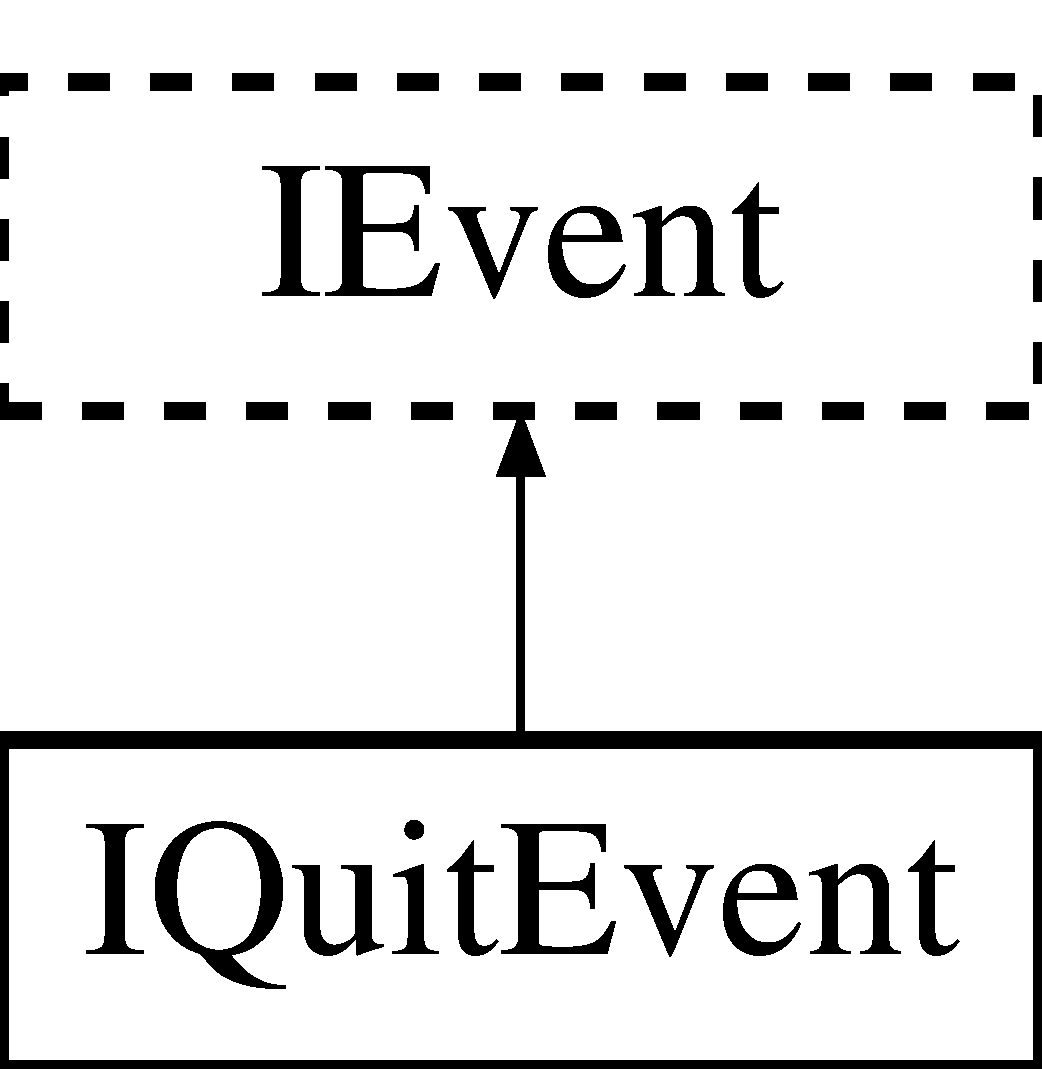
\includegraphics[height=2.000000cm]{class_i_quit_event}
\end{center}
\end{figure}
\subsection*{Additional Inherited Members}


The documentation for this class was generated from the following file\+:\begin{DoxyCompactItemize}
\item 
Code/\+Rimba/I\+Event.\+h\end{DoxyCompactItemize}

\hypertarget{class_i_render_device}{}\section{I\+Render\+Device Class Reference}
\label{class_i_render_device}\index{I\+Render\+Device@{I\+Render\+Device}}
Inheritance diagram for I\+Render\+Device\+:\begin{figure}[H]
\begin{center}
\leavevmode
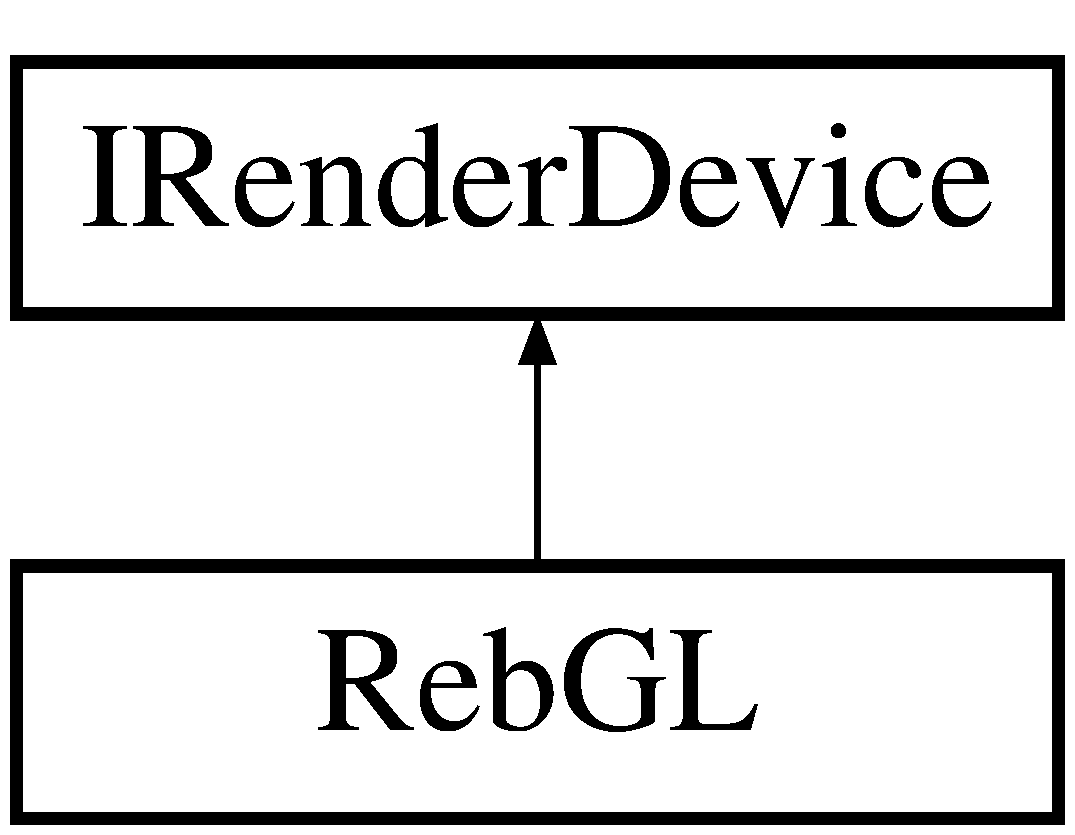
\includegraphics[height=2.000000cm]{class_i_render_device}
\end{center}
\end{figure}
\subsection*{Public Member Functions}
\begin{DoxyCompactItemize}
\item 
virtual void {\bfseries Set\+Resolution} (unsigned int w, unsigned int h)=0\hypertarget{class_i_render_device_a16610c564d6d83150e665c84f3c7f4e7}{}\label{class_i_render_device_a16610c564d6d83150e665c84f3c7f4e7}

\item 
virtual void {\bfseries Clear\+Color} (float r, float g, float b, float a)=0\hypertarget{class_i_render_device_ae943d89342c87e47aa7a20c4ea188969}{}\label{class_i_render_device_ae943d89342c87e47aa7a20c4ea188969}

\item 
virtual void {\bfseries Start\+Draw} (Methold met)=0\hypertarget{class_i_render_device_ae3b6bc5189323216fe51b46fb2d3f3f9}{}\label{class_i_render_device_ae3b6bc5189323216fe51b46fb2d3f3f9}

\item 
virtual void {\bfseries End\+Draw} ()=0\hypertarget{class_i_render_device_a85bb78a4ac85dd244d622dfd3a1507d0}{}\label{class_i_render_device_a85bb78a4ac85dd244d622dfd3a1507d0}

\item 
virtual \hyperlink{class_i_skin_manager}{I\+Skin\+Manager} $\ast$ {\bfseries Get\+Skin\+Manager} ()=0\hypertarget{class_i_render_device_af9532fb7c9230338b8aed4bf7b7a08ce}{}\label{class_i_render_device_af9532fb7c9230338b8aed4bf7b7a08ce}

\item 
virtual \hyperlink{class_i_vertex_cache_manager}{I\+Vertex\+Cache\+Manager} $\ast$ {\bfseries Get\+Vertex\+Cache\+Manager} ()=0\hypertarget{class_i_render_device_a91bfb04dc14f04af8e12303a30dd7893}{}\label{class_i_render_device_a91bfb04dc14f04af8e12303a30dd7893}

\item 
virtual \hyperlink{class_i_game_env}{I\+Game\+Env} $\ast$ {\bfseries Get\+Env} ()=0\hypertarget{class_i_render_device_aab8b22504153c63b934ef8bfd95b45bb}{}\label{class_i_render_device_aab8b22504153c63b934ef8bfd95b45bb}

\item 
virtual \hyperlink{class_i_light_system}{I\+Light\+System} $\ast$ {\bfseries Get\+Light\+System} ()=0\hypertarget{class_i_render_device_a5253dfb25d33e1f5189f5b0c0be13b1b}{}\label{class_i_render_device_a5253dfb25d33e1f5189f5b0c0be13b1b}

\item 
virtual Reb\+Matrix {\bfseries Get\+Viewport\+Mat} ()=0\hypertarget{class_i_render_device_afbb14912ab2b16f877c8c2c0a95e3d19}{}\label{class_i_render_device_afbb14912ab2b16f877c8c2c0a95e3d19}

\item 
virtual void {\bfseries Set\+Viewport\+Mat} (Reb\+Matrix svm)=0\hypertarget{class_i_render_device_a2b140ca8359f8d1db140377d63f5bcd9}{}\label{class_i_render_device_a2b140ca8359f8d1db140377d63f5bcd9}

\item 
virtual void $\ast$$\ast$ {\bfseries Get\+Viewport\+ID} ()=0\hypertarget{class_i_render_device_af5e8aac7e387d292b3d8230b9172dd2d}{}\label{class_i_render_device_af5e8aac7e387d292b3d8230b9172dd2d}

\item 
virtual void {\bfseries Get\+Viewport\+Size} (unsigned int $\ast$w, unsigned int $\ast$h)=0\hypertarget{class_i_render_device_a08eb14b6505ea5041fa0ba59be27ae95}{}\label{class_i_render_device_a08eb14b6505ea5041fa0ba59be27ae95}

\item 
virtual void {\bfseries Vertex3} (float x, float y, float z)=0\hypertarget{class_i_render_device_a3c41091e87f2a22f06f15bccb22d5bd9}{}\label{class_i_render_device_a3c41091e87f2a22f06f15bccb22d5bd9}

\item 
virtual void {\bfseries Vertex3} (Reb\+Vector RV)=0\hypertarget{class_i_render_device_a20465c217d9872d0771c2ac733894c25}{}\label{class_i_render_device_a20465c217d9872d0771c2ac733894c25}

\item 
virtual void {\bfseries Text\+Coord2} (float s, float t)=0\hypertarget{class_i_render_device_a1eff2e2033bdec9770439ed0b1549eba}{}\label{class_i_render_device_a1eff2e2033bdec9770439ed0b1549eba}

\item 
virtual void {\bfseries Bind\+Texture} (U\+I\+NT id)=0\hypertarget{class_i_render_device_afa8bd61e8f1e35aabeb682dcd9e2ba2d}{}\label{class_i_render_device_afa8bd61e8f1e35aabeb682dcd9e2ba2d}

\item 
virtual void {\bfseries Color} (float r, float g, float b)=0\hypertarget{class_i_render_device_a40b9937f1159418d167adf0c236114a8}{}\label{class_i_render_device_a40b9937f1159418d167adf0c236114a8}

\item 
virtual void {\bfseries Normal} (Reb\+Vector RV)=0\hypertarget{class_i_render_device_a6296df797d253c2c4a7e5e717356102a}{}\label{class_i_render_device_a6296df797d253c2c4a7e5e717356102a}

\item 
virtual void {\bfseries Change\+Matrix\+Mode} (Matrix\+Mode mm)=0\hypertarget{class_i_render_device_a00f9c54c3e86e413663b45b010ef5b87}{}\label{class_i_render_device_a00f9c54c3e86e413663b45b010ef5b87}

\item 
virtual void {\bfseries Clear} (bool color, bool depth)=0\hypertarget{class_i_render_device_a50f59a65c22dfb30cfd954702ef24bb5}{}\label{class_i_render_device_a50f59a65c22dfb30cfd954702ef24bb5}

\item 
virtual void {\bfseries Reset\+Matrix} ()=0\hypertarget{class_i_render_device_a0724dee30e67b687fdc8e6f2af76a55f}{}\label{class_i_render_device_a0724dee30e67b687fdc8e6f2af76a55f}

\item 
virtual void {\bfseries Push\+Matrix} ()=0\hypertarget{class_i_render_device_a6fe6908f4b6393a425749ec2d8224f26}{}\label{class_i_render_device_a6fe6908f4b6393a425749ec2d8224f26}

\item 
virtual void {\bfseries Pop\+Matrix} ()=0\hypertarget{class_i_render_device_ae10c0040ab8b874ff5fea54d7a0369e4}{}\label{class_i_render_device_ae10c0040ab8b874ff5fea54d7a0369e4}

\item 
virtual void {\bfseries Translate} (float x, float y, float z)=0\hypertarget{class_i_render_device_acc5adaf190557932ed93fd960c53a363}{}\label{class_i_render_device_acc5adaf190557932ed93fd960c53a363}

\item 
virtual void {\bfseries Rotate} (float a, float x, float y, float z)=0\hypertarget{class_i_render_device_a25c9385f2e5cb932d3f35a332f771edc}{}\label{class_i_render_device_a25c9385f2e5cb932d3f35a332f771edc}

\item 
virtual void {\bfseries Scale} (float x, float y, float z)=0\hypertarget{class_i_render_device_ad09e1ba5092cffd925d1ce724a308b49}{}\label{class_i_render_device_ad09e1ba5092cffd925d1ce724a308b49}

\item 
virtual void {\bfseries Transform\+Matrix} (Reb\+Matrix trans)=0\hypertarget{class_i_render_device_af7799d192560bbf4e87b118c27fa6f10}{}\label{class_i_render_device_af7799d192560bbf4e87b118c27fa6f10}

\item 
virtual void {\bfseries Swap} (void $\ast$window)=0\hypertarget{class_i_render_device_ab94977a2fd35735da1d303a96f39024c}{}\label{class_i_render_device_ab94977a2fd35735da1d303a96f39024c}

\item 
virtual void {\bfseries Flush} ()=0\hypertarget{class_i_render_device_ace33d49018eb3b4f120d07e73a924652}{}\label{class_i_render_device_ace33d49018eb3b4f120d07e73a924652}

\item 
virtual void {\bfseries Render} ()=0\hypertarget{class_i_render_device_aa6aff224e369de9617b9432c56c5a8be}{}\label{class_i_render_device_aa6aff224e369de9617b9432c56c5a8be}

\end{DoxyCompactItemize}


The documentation for this class was generated from the following file\+:\begin{DoxyCompactItemize}
\item 
Code/\+Rimba/I\+Render\+Device.\+h\end{DoxyCompactItemize}

\hypertarget{class_i_script_manager}{}\section{I\+Script\+Manager Class Reference}
\label{class_i_script_manager}\index{I\+Script\+Manager@{I\+Script\+Manager}}


The documentation for this class was generated from the following file\+:\begin{DoxyCompactItemize}
\item 
Code/\+Rimba/I\+Game\+Logic.\+h\end{DoxyCompactItemize}

\hypertarget{class_i_shader_program}{}\section{I\+Shader\+Program Class Reference}
\label{class_i_shader_program}\index{I\+Shader\+Program@{I\+Shader\+Program}}
Inheritance diagram for I\+Shader\+Program\+:\begin{figure}[H]
\begin{center}
\leavevmode
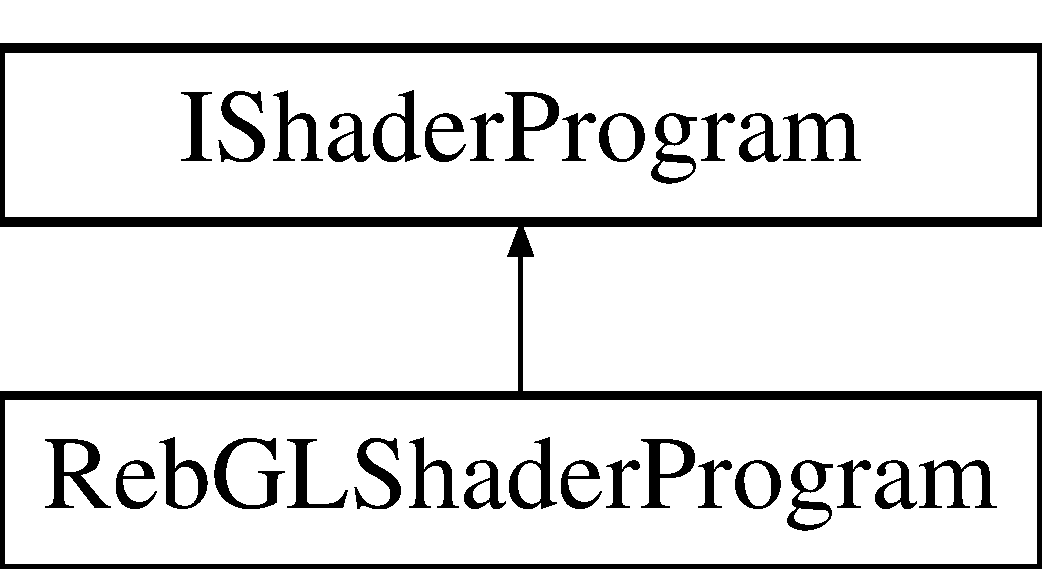
\includegraphics[height=2.000000cm]{class_i_shader_program}
\end{center}
\end{figure}


The documentation for this class was generated from the following file\+:\begin{DoxyCompactItemize}
\item 
Code/\+Rimba/I\+Render\+Device.\+h\end{DoxyCompactItemize}

\hypertarget{class_i_shader_system}{}\section{I\+Shader\+System Class Reference}
\label{class_i_shader_system}\index{I\+Shader\+System@{I\+Shader\+System}}
Inheritance diagram for I\+Shader\+System\+:\begin{figure}[H]
\begin{center}
\leavevmode
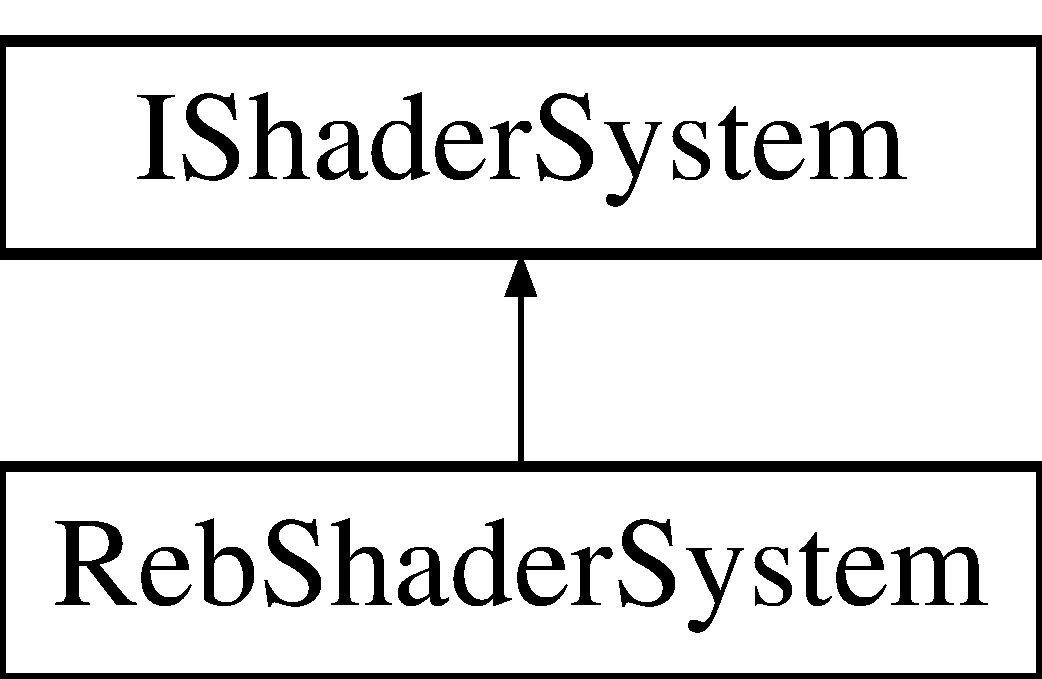
\includegraphics[height=2.000000cm]{class_i_shader_system}
\end{center}
\end{figure}
\subsection*{Public Member Functions}
\begin{DoxyCompactItemize}
\item 
virtual \hyperlink{class_i_shader_program}{I\+Shader\+Program} $\ast$ {\bfseries Get\+From\+Bank} (std\+::string name)=0\hypertarget{class_i_shader_system_a960e368e2c8f52da5b9d65ea983902ec}{}\label{class_i_shader_system_a960e368e2c8f52da5b9d65ea983902ec}

\end{DoxyCompactItemize}


The documentation for this class was generated from the following file\+:\begin{DoxyCompactItemize}
\item 
Code/\+Rimba/I\+Render\+Device.\+h\end{DoxyCompactItemize}

\hypertarget{class_i_skin_manager}{}\section{I\+Skin\+Manager Class Reference}
\label{class_i_skin_manager}\index{I\+Skin\+Manager@{I\+Skin\+Manager}}
Inheritance diagram for I\+Skin\+Manager\+:\begin{figure}[H]
\begin{center}
\leavevmode
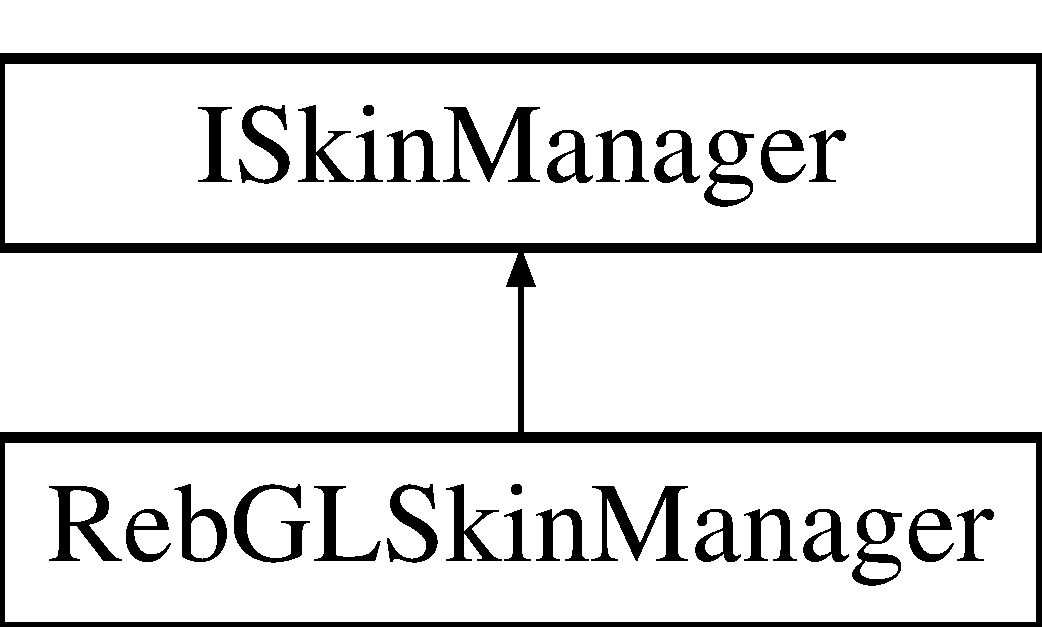
\includegraphics[height=2.000000cm]{class_i_skin_manager}
\end{center}
\end{figure}


The documentation for this class was generated from the following file\+:\begin{DoxyCompactItemize}
\item 
Code/\+Rimba/I\+Render\+Device.\+h\end{DoxyCompactItemize}

\hypertarget{class_i_sound_source}{}\section{I\+Sound\+Source Class Reference}
\label{class_i_sound_source}\index{I\+Sound\+Source@{I\+Sound\+Source}}
Inheritance diagram for I\+Sound\+Source\+:\begin{figure}[H]
\begin{center}
\leavevmode
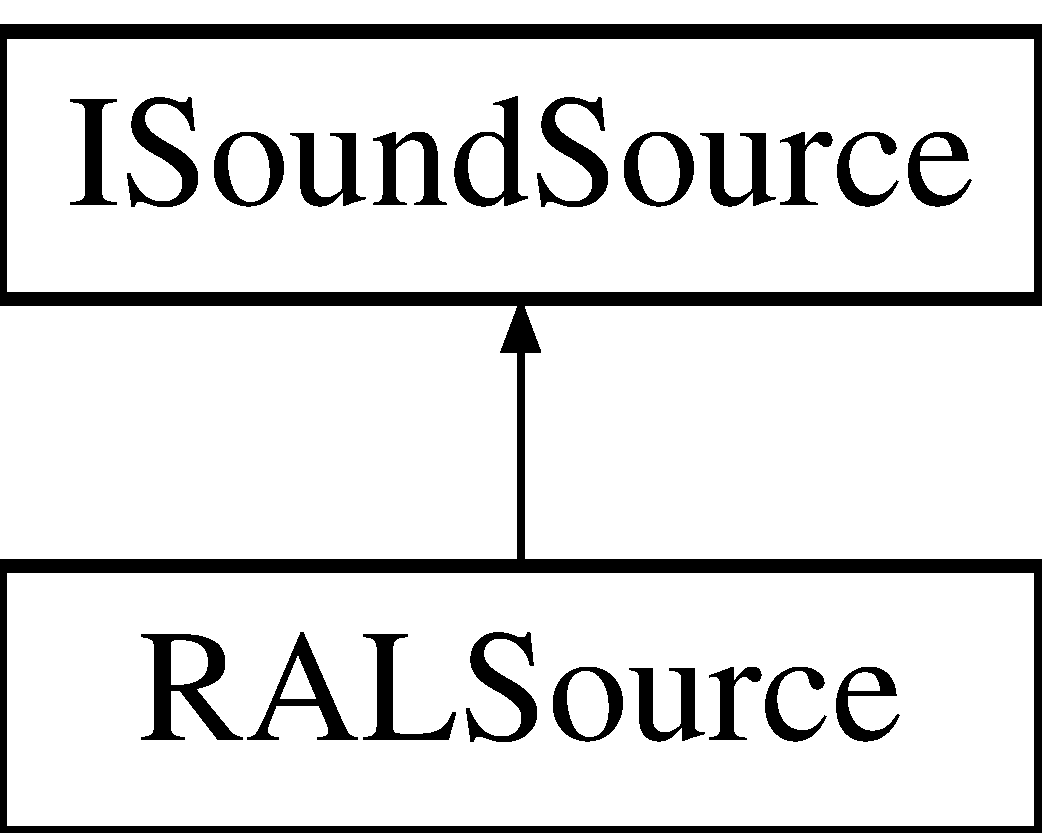
\includegraphics[height=2.000000cm]{class_i_sound_source}
\end{center}
\end{figure}


The documentation for this class was generated from the following file\+:\begin{DoxyCompactItemize}
\item 
Code/\+Reb\+Audio/I\+Audio\+Device.\+h\end{DoxyCompactItemize}

\hypertarget{class_i_sound_system}{}\section{I\+Sound\+System Class Reference}
\label{class_i_sound_system}\index{I\+Sound\+System@{I\+Sound\+System}}
Inheritance diagram for I\+Sound\+System\+:\begin{figure}[H]
\begin{center}
\leavevmode
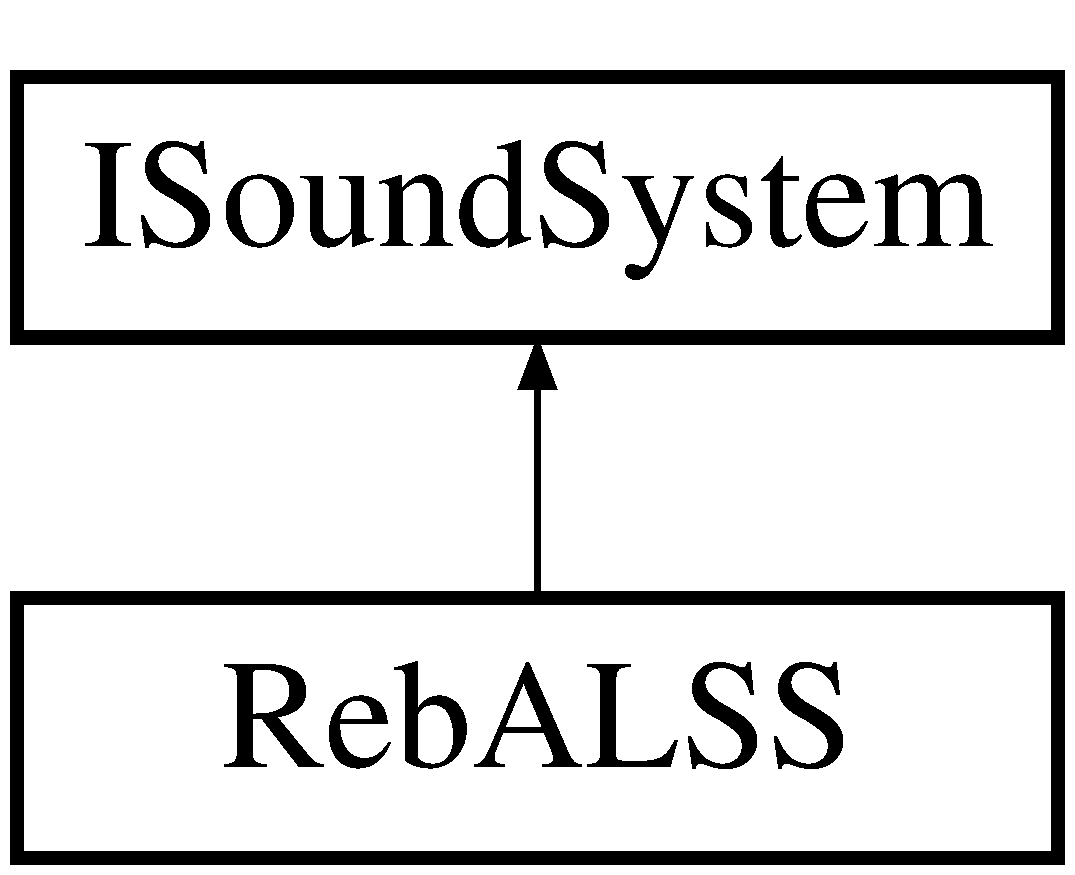
\includegraphics[height=2.000000cm]{class_i_sound_system}
\end{center}
\end{figure}
\subsection*{Public Member Functions}
\begin{DoxyCompactItemize}
\item 
virtual void {\bfseries Test} ()=0\hypertarget{class_i_sound_system_aa04e598b239727c228e8a1b42472c7f8}{}\label{class_i_sound_system_aa04e598b239727c228e8a1b42472c7f8}

\item 
virtual void {\bfseries Update} ()\hypertarget{class_i_sound_system_a2ea341684112c605f9ba72c195a46f51}{}\label{class_i_sound_system_a2ea341684112c605f9ba72c195a46f51}

\item 
virtual void {\bfseries Test} ()=0\hypertarget{class_i_sound_system_aa04e598b239727c228e8a1b42472c7f8}{}\label{class_i_sound_system_aa04e598b239727c228e8a1b42472c7f8}

\item 
virtual void {\bfseries Update} ()\hypertarget{class_i_sound_system_a2ea341684112c605f9ba72c195a46f51}{}\label{class_i_sound_system_a2ea341684112c605f9ba72c195a46f51}

\end{DoxyCompactItemize}


The documentation for this class was generated from the following file\+:\begin{DoxyCompactItemize}
\item 
Code/\+Reb\+Audio/I\+Audio\+Device.\+h\end{DoxyCompactItemize}

\hypertarget{class_i_terrain}{}\section{I\+Terrain Class Reference}
\label{class_i_terrain}\index{I\+Terrain@{I\+Terrain}}
Inheritance diagram for I\+Terrain\+:\begin{figure}[H]
\begin{center}
\leavevmode
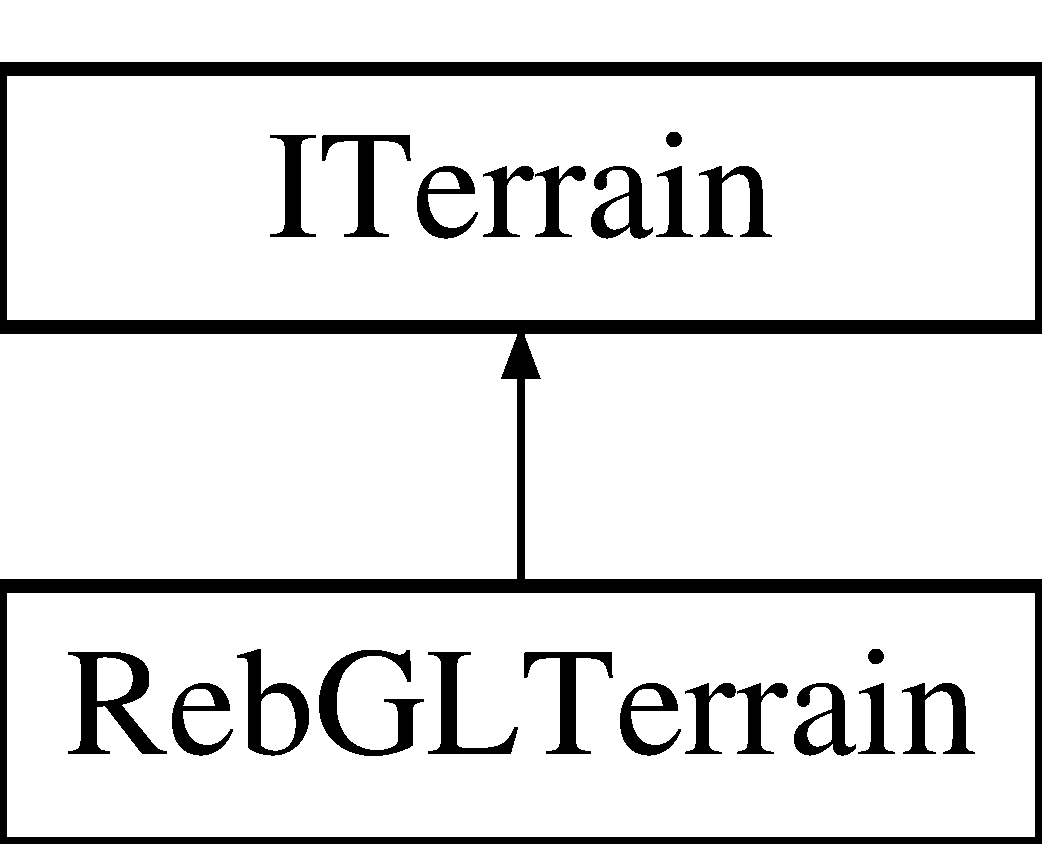
\includegraphics[height=2.000000cm]{class_i_terrain}
\end{center}
\end{figure}
\subsection*{Public Member Functions}
\begin{DoxyCompactItemize}
\item 
virtual void {\bfseries Draw} ()=0\hypertarget{class_i_terrain_aceb37ac603eeebde3d1c0125114d648d}{}\label{class_i_terrain_aceb37ac603eeebde3d1c0125114d648d}

\item 
virtual Reb\+Matrix {\bfseries Get\+Trans} ()=0\hypertarget{class_i_terrain_a1fc14310d1f3a3e72453a39de16e8668}{}\label{class_i_terrain_a1fc14310d1f3a3e72453a39de16e8668}

\end{DoxyCompactItemize}


The documentation for this class was generated from the following file\+:\begin{DoxyCompactItemize}
\item 
Code/\+Rimba/Reb\+Graphic\+Elements.\+h\end{DoxyCompactItemize}

\hypertarget{class_i_texture}{}\section{I\+Texture Class Reference}
\label{class_i_texture}\index{I\+Texture@{I\+Texture}}
Inheritance diagram for I\+Texture\+:\begin{figure}[H]
\begin{center}
\leavevmode
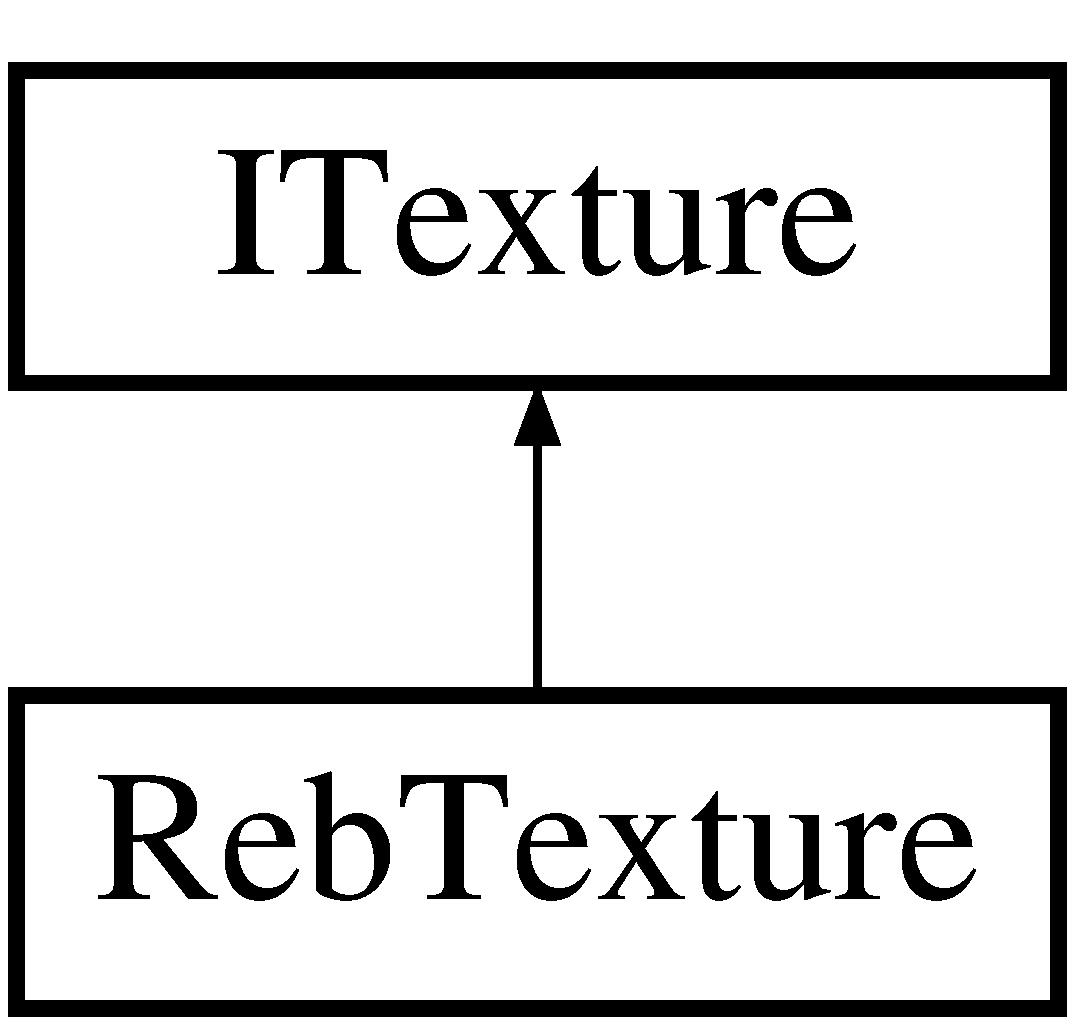
\includegraphics[height=2.000000cm]{class_i_texture}
\end{center}
\end{figure}
\subsection*{Public Member Functions}
\begin{DoxyCompactItemize}
\item 
virtual \hyperlink{class_reb_file}{Reb\+File} $\ast$ {\bfseries Get\+File} ()=0\hypertarget{class_i_texture_a0e385878f3625e9e8a8144eb3f6ae08e}{}\label{class_i_texture_a0e385878f3625e9e8a8144eb3f6ae08e}

\item 
virtual void {\bfseries Bind} ()=0\hypertarget{class_i_texture_ac25f84578ea49ae8e56cc7c98606740f}{}\label{class_i_texture_ac25f84578ea49ae8e56cc7c98606740f}

\end{DoxyCompactItemize}


The documentation for this class was generated from the following file\+:\begin{DoxyCompactItemize}
\item 
Code/\+Rimba/Reb\+Graphic\+Elements.\+h\end{DoxyCompactItemize}

\hypertarget{class_i_u_i_system}{}\section{I\+U\+I\+System Class Reference}
\label{class_i_u_i_system}\index{I\+U\+I\+System@{I\+U\+I\+System}}


The documentation for this class was generated from the following file\+:\begin{DoxyCompactItemize}
\item 
Code/\+Rimba/I\+U\+I\+System.\+h\end{DoxyCompactItemize}

\hypertarget{class_i_vertex_buffer}{}\section{I\+Vertex\+Buffer Class Reference}
\label{class_i_vertex_buffer}\index{I\+Vertex\+Buffer@{I\+Vertex\+Buffer}}
Inheritance diagram for I\+Vertex\+Buffer\+:\begin{figure}[H]
\begin{center}
\leavevmode
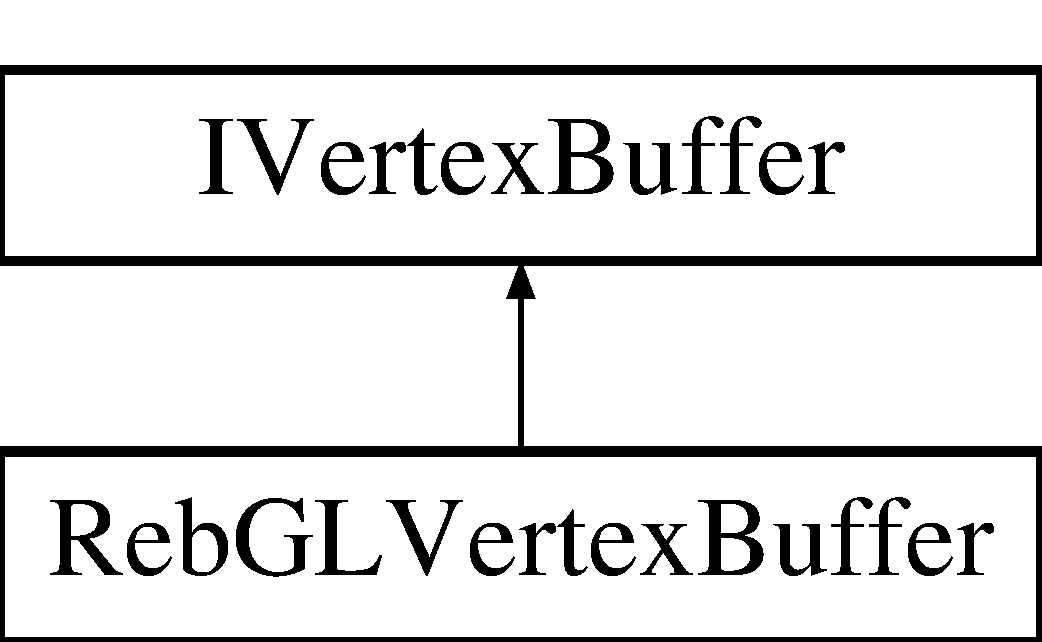
\includegraphics[height=2.000000cm]{class_i_vertex_buffer}
\end{center}
\end{figure}
\subsection*{Public Member Functions}
\begin{DoxyCompactItemize}
\item 
virtual std\+::vector$<$ Reb\+Vector $>$ $\ast$ {\bfseries Get\+Vertices} ()=0\hypertarget{class_i_vertex_buffer_ac3ebbfc832e42aeb21afa54f636f4945}{}\label{class_i_vertex_buffer_ac3ebbfc832e42aeb21afa54f636f4945}

\item 
virtual std\+::vector$<$ Reb\+Vector $>$ $\ast$ {\bfseries Get\+Normals} ()=0\hypertarget{class_i_vertex_buffer_adec6f810ef964c3043023cabaa6a9875}{}\label{class_i_vertex_buffer_adec6f810ef964c3043023cabaa6a9875}

\item 
virtual std\+::vector$<$ Reb\+Vector $>$ $\ast$ {\bfseries Get\+Texture\+Coords} ()=0\hypertarget{class_i_vertex_buffer_a6a1376c2473d0863d23c7a28ff664c32}{}\label{class_i_vertex_buffer_a6a1376c2473d0863d23c7a28ff664c32}

\item 
virtual void {\bfseries Set\+Renderable} (bool s)=0\hypertarget{class_i_vertex_buffer_a1a56478b0998b0ccd6d3f10f1231ac06}{}\label{class_i_vertex_buffer_a1a56478b0998b0ccd6d3f10f1231ac06}

\item 
virtual bool {\bfseries is\+Renderable} ()=0\hypertarget{class_i_vertex_buffer_a46768c41e96e5815cf932d2c9979a970}{}\label{class_i_vertex_buffer_a46768c41e96e5815cf932d2c9979a970}

\item 
virtual \hyperlink{class_i_material}{I\+Material} $\ast$ {\bfseries Get\+Material} ()=0\hypertarget{class_i_vertex_buffer_ae3632b82fc09404a9e09a520d6da4d5d}{}\label{class_i_vertex_buffer_ae3632b82fc09404a9e09a520d6da4d5d}

\item 
virtual void {\bfseries Draw} ()=0\hypertarget{class_i_vertex_buffer_ae8e72db479d6cbe32620307f58babb6a}{}\label{class_i_vertex_buffer_ae8e72db479d6cbe32620307f58babb6a}

\item 
virtual void {\bfseries Set\+Name} (std\+::string sname)=0\hypertarget{class_i_vertex_buffer_ad0b387d86e6ed76df6684c60c4ae43da}{}\label{class_i_vertex_buffer_ad0b387d86e6ed76df6684c60c4ae43da}

\item 
virtual void {\bfseries Set\+Trans} (Reb\+Matrix set)=0\hypertarget{class_i_vertex_buffer_acd36b826ab021f1271ff34f87b55fd45}{}\label{class_i_vertex_buffer_acd36b826ab021f1271ff34f87b55fd45}

\item 
virtual Reb\+Matrix $\ast$ {\bfseries Get\+Trans} ()=0\hypertarget{class_i_vertex_buffer_ae714edc6a19dbd299307b9d94bd45dcc}{}\label{class_i_vertex_buffer_ae714edc6a19dbd299307b9d94bd45dcc}

\item 
virtual void {\bfseries Set\+Material} (\hyperlink{class_i_material}{I\+Material} $\ast$set)=0\hypertarget{class_i_vertex_buffer_a5284c66108278f369ac612c239720812}{}\label{class_i_vertex_buffer_a5284c66108278f369ac612c239720812}

\end{DoxyCompactItemize}


The documentation for this class was generated from the following file\+:\begin{DoxyCompactItemize}
\item 
Code/\+Rimba/Reb\+Graphic\+Elements.\+h\end{DoxyCompactItemize}

\hypertarget{class_i_vertex_cache}{}\section{I\+Vertex\+Cache Class Reference}
\label{class_i_vertex_cache}\index{I\+Vertex\+Cache@{I\+Vertex\+Cache}}
Inheritance diagram for I\+Vertex\+Cache\+:\begin{figure}[H]
\begin{center}
\leavevmode
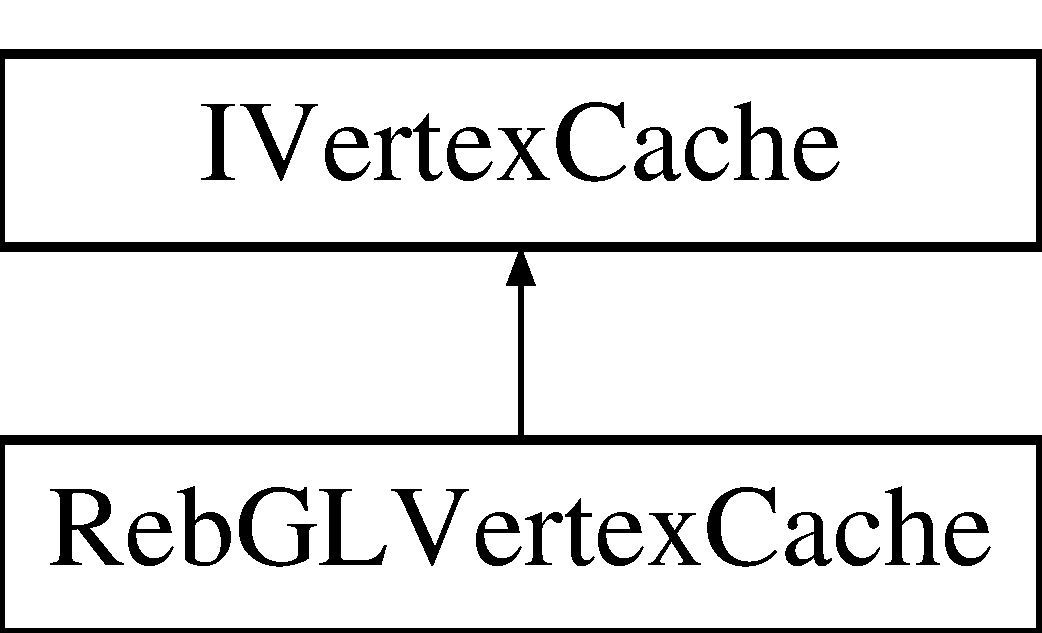
\includegraphics[height=2.000000cm]{class_i_vertex_cache}
\end{center}
\end{figure}
\subsection*{Public Member Functions}
\begin{DoxyCompactItemize}
\item 
virtual void {\bfseries Add\+Buffer} (\hyperlink{class_i_vertex_buffer}{I\+Vertex\+Buffer} $\ast$abuff)=0\hypertarget{class_i_vertex_cache_ad74aab900cfede6e8578e5aa084a8c7b}{}\label{class_i_vertex_cache_ad74aab900cfede6e8578e5aa084a8c7b}

\item 
virtual void {\bfseries Set\+Name} (std\+::string sname)=0\hypertarget{class_i_vertex_cache_a2090b2ccdb47167ef849b05702750094}{}\label{class_i_vertex_cache_a2090b2ccdb47167ef849b05702750094}

\item 
virtual std\+::string {\bfseries Get\+Name} ()=0\hypertarget{class_i_vertex_cache_aeb63d8e35221a65ec16f32f71a7845cf}{}\label{class_i_vertex_cache_aeb63d8e35221a65ec16f32f71a7845cf}

\item 
virtual std\+::string {\bfseries Get\+File\+Name} ()=0\hypertarget{class_i_vertex_cache_ad855ca8c19730278e77069bff61bc2bb}{}\label{class_i_vertex_cache_ad855ca8c19730278e77069bff61bc2bb}

\item 
virtual std\+::vector$<$ \hyperlink{class_i_vertex_buffer}{I\+Vertex\+Buffer} $\ast$ $>$ $\ast$ {\bfseries Get\+R\+V\+Bs} ()=0\hypertarget{class_i_vertex_cache_af6cde66375db3096d66e5e643948b02c}{}\label{class_i_vertex_cache_af6cde66375db3096d66e5e643948b02c}

\item 
virtual void {\bfseries Set\+Trans} (Reb\+Matrix set)=0\hypertarget{class_i_vertex_cache_a327bdb047f2cae1c589948bcca05dd1f}{}\label{class_i_vertex_cache_a327bdb047f2cae1c589948bcca05dd1f}

\item 
virtual Reb\+Matrix $\ast$ {\bfseries Get\+Trans} ()=0\hypertarget{class_i_vertex_cache_ab0c3f7853e463997a11be180fdd2cf8f}{}\label{class_i_vertex_cache_ab0c3f7853e463997a11be180fdd2cf8f}

\item 
virtual void {\bfseries Set\+File\+Name} (std\+::string sfname)=0\hypertarget{class_i_vertex_cache_a8f09c3a581da7a403317d12312985350}{}\label{class_i_vertex_cache_a8f09c3a581da7a403317d12312985350}

\item 
virtual void {\bfseries Delete\+Buffer} (U\+I\+NT V\+B\+ID)=0\hypertarget{class_i_vertex_cache_abd31eb5c1814d1680fc0f3d69f3e363a}{}\label{class_i_vertex_cache_abd31eb5c1814d1680fc0f3d69f3e363a}

\end{DoxyCompactItemize}


The documentation for this class was generated from the following file\+:\begin{DoxyCompactItemize}
\item 
Code/\+Rimba/Reb\+Graphic\+Elements.\+h\end{DoxyCompactItemize}

\hypertarget{class_i_vertex_cache_manager}{}\section{I\+Vertex\+Cache\+Manager Class Reference}
\label{class_i_vertex_cache_manager}\index{I\+Vertex\+Cache\+Manager@{I\+Vertex\+Cache\+Manager}}
Inheritance diagram for I\+Vertex\+Cache\+Manager\+:\begin{figure}[H]
\begin{center}
\leavevmode
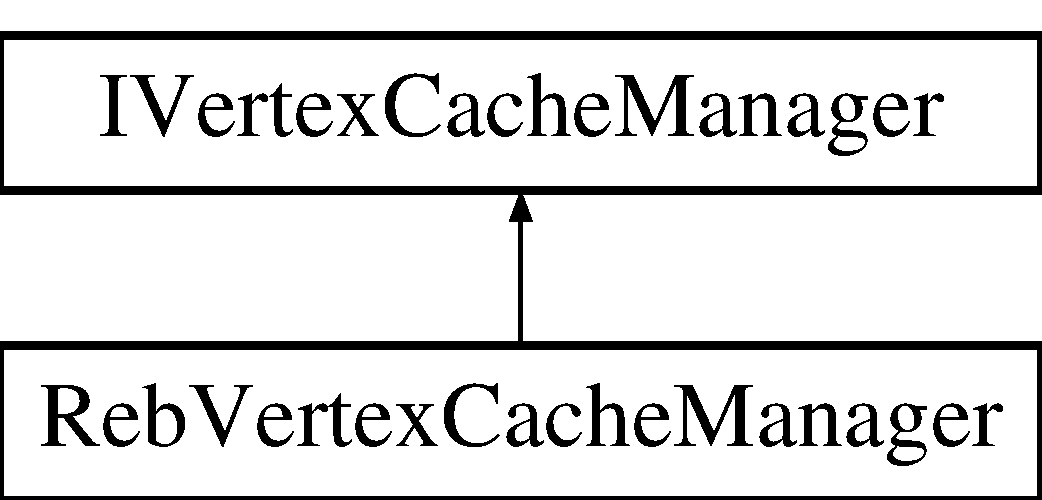
\includegraphics[height=2.000000cm]{class_i_vertex_cache_manager}
\end{center}
\end{figure}
\subsection*{Public Member Functions}
\begin{DoxyCompactItemize}
\item 
virtual void {\bfseries Create\+Cache} (std\+::string name, std\+::vector$<$ \hyperlink{class_i_vertex_buffer}{I\+Vertex\+Buffer} $>$ R\+VB)=0\hypertarget{class_i_vertex_cache_manager_a75ecdec282d26db77e596316208a2060}{}\label{class_i_vertex_cache_manager_a75ecdec282d26db77e596316208a2060}

\item 
virtual void {\bfseries Delete\+Cache} (\hyperlink{class_i_vertex_cache}{I\+Vertex\+Cache} $\ast$rvc)=0\hypertarget{class_i_vertex_cache_manager_afd26ce03ebe670b22e027636239ff0ab}{}\label{class_i_vertex_cache_manager_afd26ce03ebe670b22e027636239ff0ab}

\item 
virtual \hyperlink{class_i_vertex_cache}{I\+Vertex\+Cache} $\ast$ {\bfseries Get\+Vertex\+Cache} (std\+::string cname)=0\hypertarget{class_i_vertex_cache_manager_affefebf1a1b734c79cccd4d6fcb06e28}{}\label{class_i_vertex_cache_manager_affefebf1a1b734c79cccd4d6fcb06e28}

\item 
virtual \hyperlink{class_i_vertex_cache}{I\+Vertex\+Cache} $\ast$ {\bfseries Get\+V\+C\+By\+File} (std\+::string filename)=0\hypertarget{class_i_vertex_cache_manager_abc3a2b2201210994074a9aa3ba4f413c}{}\label{class_i_vertex_cache_manager_abc3a2b2201210994074a9aa3ba4f413c}

\item 
virtual void {\bfseries Create\+Cache\+From\+File} (std\+::string cname, \hyperlink{class_reb_file}{Reb\+File} $\ast$file)=0\hypertarget{class_i_vertex_cache_manager_a9cb416e026f024de88f05558b58492bd}{}\label{class_i_vertex_cache_manager_a9cb416e026f024de88f05558b58492bd}

\item 
virtual void {\bfseries Release} ()=0\hypertarget{class_i_vertex_cache_manager_a963ff6d6dea612671cb5b49922d4359e}{}\label{class_i_vertex_cache_manager_a963ff6d6dea612671cb5b49922d4359e}

\item 
virtual std\+::vector$<$ \hyperlink{class_i_vertex_cache}{I\+Vertex\+Cache} $\ast$ $>$ $\ast$ {\bfseries Get\+R\+V\+Cs} ()=0\hypertarget{class_i_vertex_cache_manager_a5796a512336d9c2b18d55f5f39b6ad36}{}\label{class_i_vertex_cache_manager_a5796a512336d9c2b18d55f5f39b6ad36}

\end{DoxyCompactItemize}


The documentation for this class was generated from the following file\+:\begin{DoxyCompactItemize}
\item 
Code/\+Rimba/I\+Render\+Device.\+h\end{DoxyCompactItemize}

\hypertarget{class_i_w_a_e_m}{}\section{I\+W\+A\+EM Class Reference}
\label{class_i_w_a_e_m}\index{I\+W\+A\+EM@{I\+W\+A\+EM}}
Inheritance diagram for I\+W\+A\+EM\+:\begin{figure}[H]
\begin{center}
\leavevmode
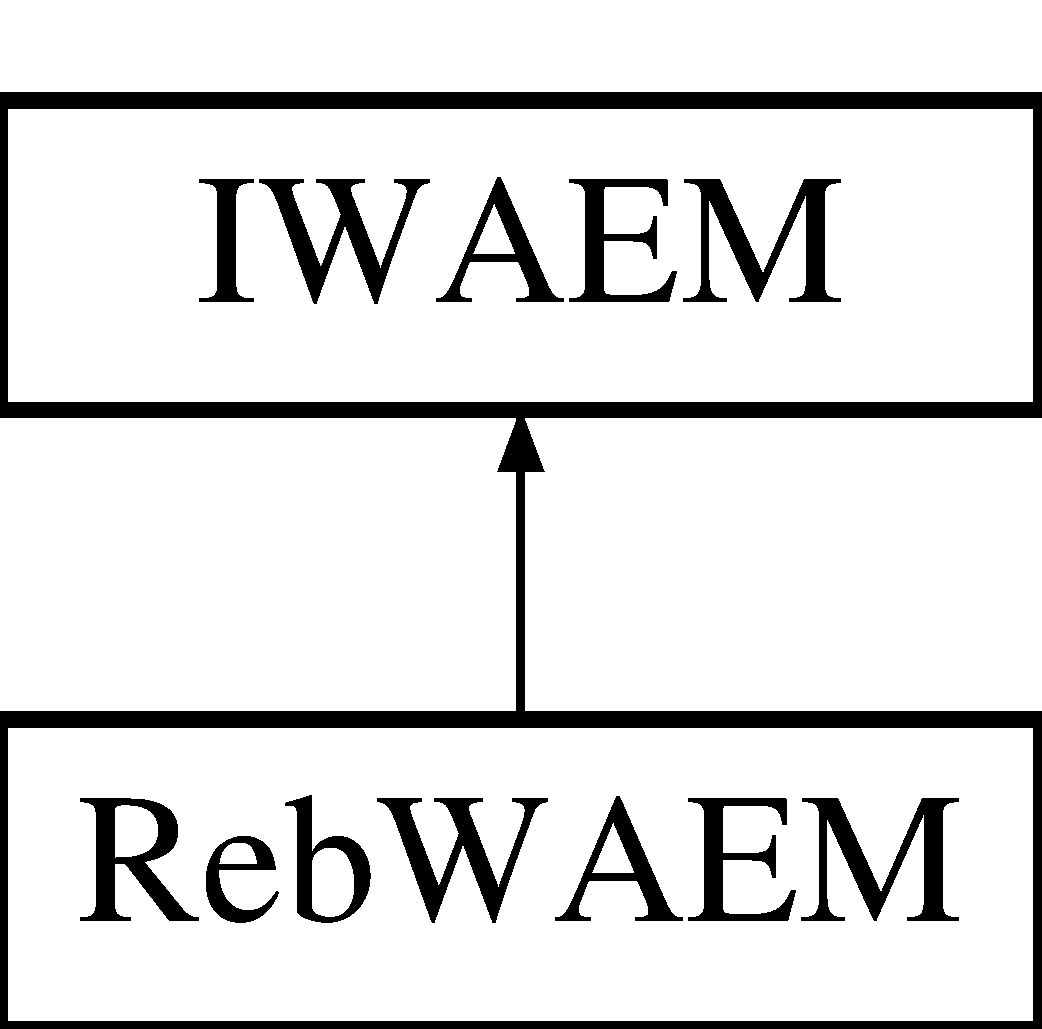
\includegraphics[height=2.000000cm]{class_i_w_a_e_m}
\end{center}
\end{figure}
\subsection*{Public Member Functions}
\begin{DoxyCompactItemize}
\item 
virtual \hyperlink{class_i_window}{I\+Window} $\ast$ {\bfseries Create\+Wnd} (std\+::string name, int sx, int sy, bool fullscreen=false, int posx=0, int posy=0)=0\hypertarget{class_i_w_a_e_m_a7708fc1d3a6f839100749d8b5d985ede}{}\label{class_i_w_a_e_m_a7708fc1d3a6f839100749d8b5d985ede}

\item 
virtual \hyperlink{class_i_window}{I\+Window} $\ast$ {\bfseries Get\+By\+Name} (std\+::string name)=0\hypertarget{class_i_w_a_e_m_a180cd608c682ca5a78c1c91c98f12b29}{}\label{class_i_w_a_e_m_a180cd608c682ca5a78c1c91c98f12b29}

\item 
virtual void {\bfseries Delete\+Window} (\hyperlink{class_i_window}{I\+Window} $\ast$win)=0\hypertarget{class_i_w_a_e_m_a9ec07af32081c3e934eeb23fd9f65fb4}{}\label{class_i_w_a_e_m_a9ec07af32081c3e934eeb23fd9f65fb4}

\item 
virtual void {\bfseries Register\+Event\+Listener} (\hyperlink{class_i_event_listener}{I\+Event\+Listener} $\ast$toreg)=0\hypertarget{class_i_w_a_e_m_a74c644610999df689b1fc30abc717fb2}{}\label{class_i_w_a_e_m_a74c644610999df689b1fc30abc717fb2}

\item 
virtual void {\bfseries Un\+Register\+Event\+Listener} (\hyperlink{class_i_event_listener}{I\+Event\+Listener} $\ast$tounreg)=0\hypertarget{class_i_w_a_e_m_acbea005c19162f0236d1496d294f7cf1}{}\label{class_i_w_a_e_m_acbea005c19162f0236d1496d294f7cf1}

\item 
virtual void {\bfseries Get\+Event} ()=0\hypertarget{class_i_w_a_e_m_a310cf816fe820cb7eb261dea912b2a65}{}\label{class_i_w_a_e_m_a310cf816fe820cb7eb261dea912b2a65}

\end{DoxyCompactItemize}


The documentation for this class was generated from the following file\+:\begin{DoxyCompactItemize}
\item 
Code/\+Rimba/I\+W\+A\+E\+M.\+h\end{DoxyCompactItemize}

\hypertarget{class_i_window}{}\section{I\+Window Class Reference}
\label{class_i_window}\index{I\+Window@{I\+Window}}
Inheritance diagram for I\+Window\+:\begin{figure}[H]
\begin{center}
\leavevmode
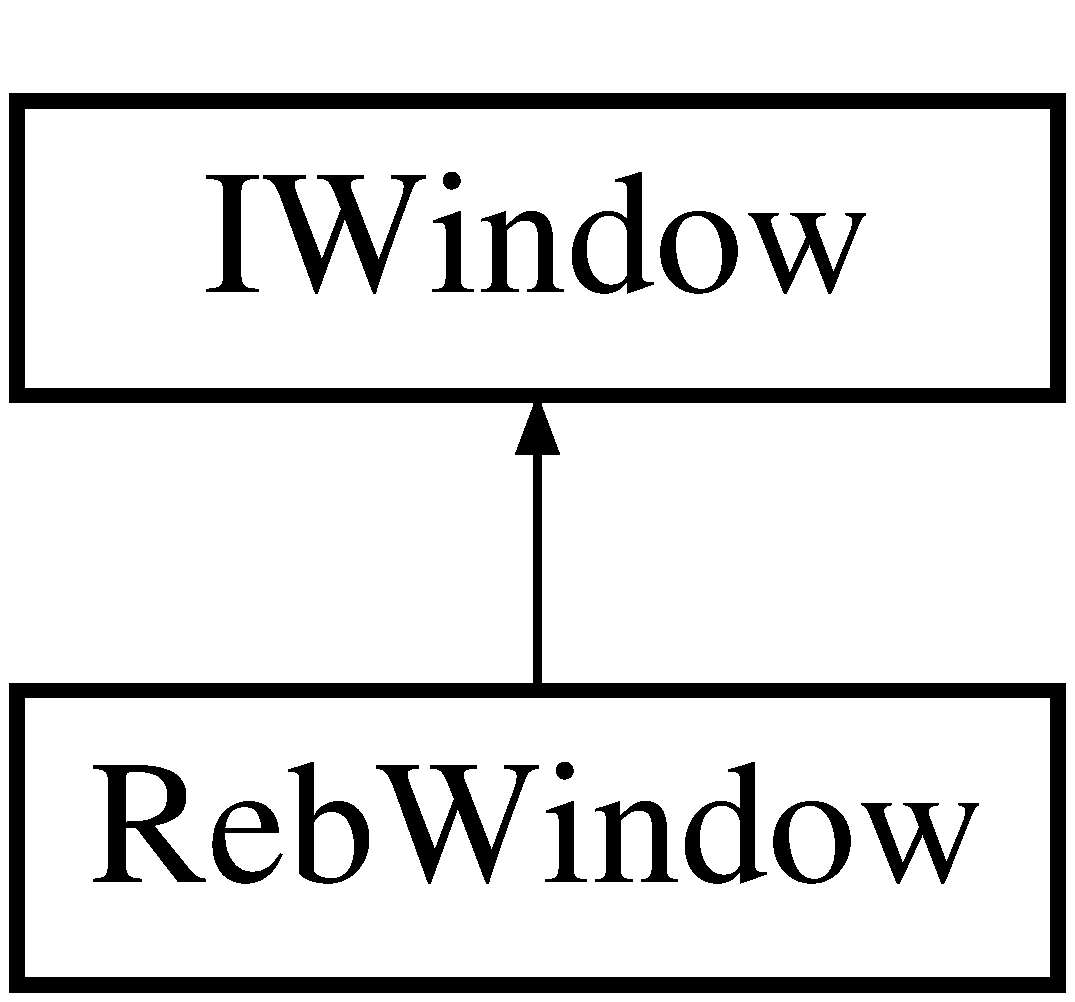
\includegraphics[height=2.000000cm]{class_i_window}
\end{center}
\end{figure}
\subsection*{Public Member Functions}
\begin{DoxyCompactItemize}
\item 
virtual std\+::string {\bfseries Get\+Name} ()=0\hypertarget{class_i_window_a153877b9f3d15eaaacd9d6d81513635a}{}\label{class_i_window_a153877b9f3d15eaaacd9d6d81513635a}

\item 
virtual void {\bfseries Create\+G\+L\+Context} ()=0\hypertarget{class_i_window_a9463fe4132cbcce240365e7299bbf8ea}{}\label{class_i_window_a9463fe4132cbcce240365e7299bbf8ea}

\item 
virtual void {\bfseries Set\+Size} (int w, int h)=0\hypertarget{class_i_window_ad93f236da8028020d5adb3df2e54b229}{}\label{class_i_window_ad93f236da8028020d5adb3df2e54b229}

\item 
virtual void {\bfseries Get\+Size} (int $\ast$w, int $\ast$h)=0\hypertarget{class_i_window_a2ed48de2a80cff398aa1abeb428847ca}{}\label{class_i_window_a2ed48de2a80cff398aa1abeb428847ca}

\item 
virtual void {\bfseries Set\+Full\+Screen} (bool fs)=0\hypertarget{class_i_window_ad0a4a80c0c556df1a42cfd04e56ad4c4}{}\label{class_i_window_ad0a4a80c0c556df1a42cfd04e56ad4c4}

\item 
virtual void {\bfseries Swap\+Buff} ()=0\hypertarget{class_i_window_adff844ec87f9cce2a84ea69bde3c7182}{}\label{class_i_window_adff844ec87f9cce2a84ea69bde3c7182}

\end{DoxyCompactItemize}


The documentation for this class was generated from the following file\+:\begin{DoxyCompactItemize}
\item 
Code/\+Rimba/I\+W\+A\+E\+M.\+h\end{DoxyCompactItemize}

\hypertarget{class_i_window_manager}{}\section{I\+Window\+Manager Class Reference}
\label{class_i_window_manager}\index{I\+Window\+Manager@{I\+Window\+Manager}}
Inheritance diagram for I\+Window\+Manager\+:\begin{figure}[H]
\begin{center}
\leavevmode
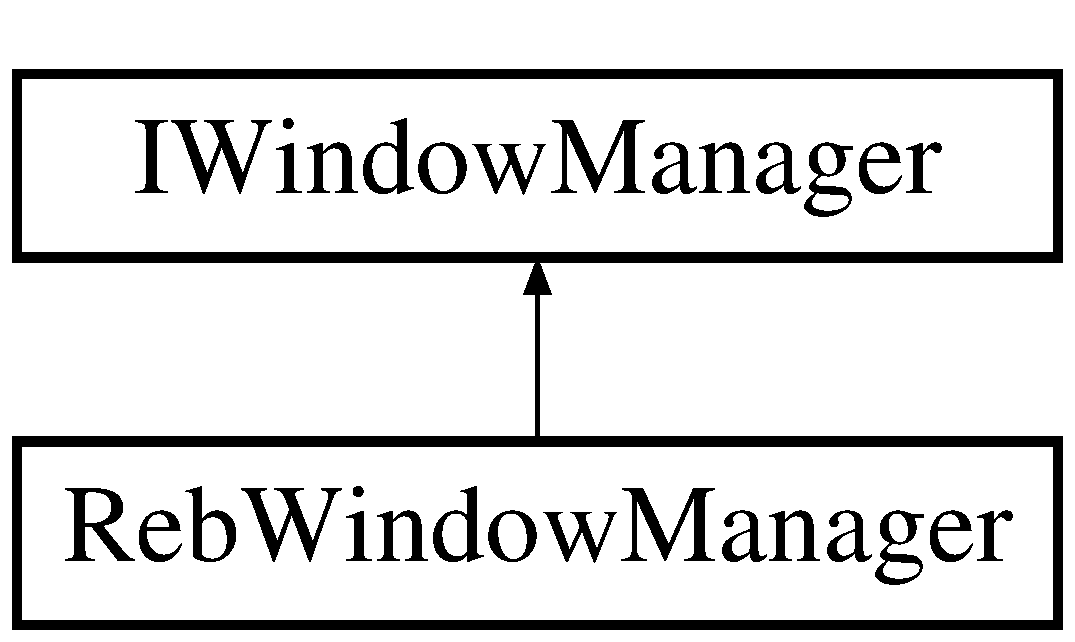
\includegraphics[height=2.000000cm]{class_i_window_manager}
\end{center}
\end{figure}
\subsection*{Public Member Functions}
\begin{DoxyCompactItemize}
\item 
virtual void {\bfseries Init} ()=0\hypertarget{class_i_window_manager_a43e41076eb824b0e52dde29a28db9df8}{}\label{class_i_window_manager_a43e41076eb824b0e52dde29a28db9df8}

\item 
virtual void {\bfseries Release} ()=0\hypertarget{class_i_window_manager_afa49e2a263b7690f2b0745c0534198c8}{}\label{class_i_window_manager_afa49e2a263b7690f2b0745c0534198c8}

\item 
virtual void {\bfseries Create\+Win} (std\+::string name, int w, int h, int posx=0, int posy=0)=0\hypertarget{class_i_window_manager_a721402c56e32650d79fc85982708c991}{}\label{class_i_window_manager_a721402c56e32650d79fc85982708c991}

\item 
virtual void {\bfseries Destroy\+Window} (std\+::string name)=0\hypertarget{class_i_window_manager_aced5a16a6f3f645cbfa3421b20f2bcdb}{}\label{class_i_window_manager_aced5a16a6f3f645cbfa3421b20f2bcdb}

\item 
virtual void $\ast$ {\bfseries Get\+Window} (std\+::string name)=0\hypertarget{class_i_window_manager_a3197d118b10af0d714881c81658ac6da}{}\label{class_i_window_manager_a3197d118b10af0d714881c81658ac6da}

\item 
virtual void {\bfseries Enable\+Render} (std\+::string name)=0\hypertarget{class_i_window_manager_a53ce6ab8759917bba298f8b5146724d0}{}\label{class_i_window_manager_a53ce6ab8759917bba298f8b5146724d0}

\item 
virtual void {\bfseries Swap\+Window} (void $\ast$window)=0\hypertarget{class_i_window_manager_a81d1183a1050b52e9a11fc77b9b297b7}{}\label{class_i_window_manager_a81d1183a1050b52e9a11fc77b9b297b7}

\item 
virtual void {\bfseries Disable\+Render} (std\+::string name)=0\hypertarget{class_i_window_manager_ae639c7c7a6de9a41c2179e61abbf1408}{}\label{class_i_window_manager_ae639c7c7a6de9a41c2179e61abbf1408}

\item 
virtual void {\bfseries Trap\+Mouse} (bool trap)=0\hypertarget{class_i_window_manager_aef2c326099c719fa84afa20c87b156d2}{}\label{class_i_window_manager_aef2c326099c719fa84afa20c87b156d2}

\item 
virtual void {\bfseries Init} ()=0\hypertarget{class_i_window_manager_a43e41076eb824b0e52dde29a28db9df8}{}\label{class_i_window_manager_a43e41076eb824b0e52dde29a28db9df8}

\item 
virtual void {\bfseries Release} ()=0\hypertarget{class_i_window_manager_afa49e2a263b7690f2b0745c0534198c8}{}\label{class_i_window_manager_afa49e2a263b7690f2b0745c0534198c8}

\item 
virtual void {\bfseries Create\+Win} (std\+::string name, int w, int h, int posx=0, int posy=0)=0\hypertarget{class_i_window_manager_a721402c56e32650d79fc85982708c991}{}\label{class_i_window_manager_a721402c56e32650d79fc85982708c991}

\item 
virtual void {\bfseries Destroy\+Window} (std\+::string name)=0\hypertarget{class_i_window_manager_aced5a16a6f3f645cbfa3421b20f2bcdb}{}\label{class_i_window_manager_aced5a16a6f3f645cbfa3421b20f2bcdb}

\item 
virtual void $\ast$ {\bfseries Get\+Window} (std\+::string name)=0\hypertarget{class_i_window_manager_a3197d118b10af0d714881c81658ac6da}{}\label{class_i_window_manager_a3197d118b10af0d714881c81658ac6da}

\item 
virtual void {\bfseries Enable\+Render} (std\+::string name)=0\hypertarget{class_i_window_manager_a53ce6ab8759917bba298f8b5146724d0}{}\label{class_i_window_manager_a53ce6ab8759917bba298f8b5146724d0}

\item 
virtual void {\bfseries Swap\+Window} (void $\ast$window)=0\hypertarget{class_i_window_manager_a81d1183a1050b52e9a11fc77b9b297b7}{}\label{class_i_window_manager_a81d1183a1050b52e9a11fc77b9b297b7}

\item 
virtual void {\bfseries Disable\+Render} (std\+::string name)=0\hypertarget{class_i_window_manager_ae639c7c7a6de9a41c2179e61abbf1408}{}\label{class_i_window_manager_ae639c7c7a6de9a41c2179e61abbf1408}

\item 
virtual void {\bfseries Trap\+Mouse} (bool trap)=0\hypertarget{class_i_window_manager_aef2c326099c719fa84afa20c87b156d2}{}\label{class_i_window_manager_aef2c326099c719fa84afa20c87b156d2}

\end{DoxyCompactItemize}


The documentation for this class was generated from the following file\+:\begin{DoxyCompactItemize}
\item 
Code/\+Reb\+Window/I\+Window\+Manager.\+h\end{DoxyCompactItemize}

\hypertarget{struct_l_m_struct}{}\section{L\+M\+Struct Struct Reference}
\label{struct_l_m_struct}\index{L\+M\+Struct@{L\+M\+Struct}}
\subsection*{Public Attributes}
\begin{DoxyCompactItemize}
\item 
G\+Luint {\bfseries D}\hypertarget{struct_l_m_struct_ad1d582ce9c80db4310f23bd7c478ce89}{}\label{struct_l_m_struct_ad1d582ce9c80db4310f23bd7c478ce89}

\item 
G\+Luint {\bfseries A}\hypertarget{struct_l_m_struct_ac4bee4c141c9f7f08c2b39f70cf9e479}{}\label{struct_l_m_struct_ac4bee4c141c9f7f08c2b39f70cf9e479}

\item 
G\+Luint {\bfseries S}\hypertarget{struct_l_m_struct_a68f6c6514283ae0fda24037968c70a72}{}\label{struct_l_m_struct_a68f6c6514283ae0fda24037968c70a72}

\end{DoxyCompactItemize}


The documentation for this struct was generated from the following file\+:\begin{DoxyCompactItemize}
\item 
Code/\+Reb\+G\+L/Reb\+G\+L\+\_\+\+S\+S.\+h\end{DoxyCompactItemize}

\hypertarget{classtinyxml2_1_1_mem_pool}{}\section{tinyxml2\+:\+:Mem\+Pool Class Reference}
\label{classtinyxml2_1_1_mem_pool}\index{tinyxml2\+::\+Mem\+Pool@{tinyxml2\+::\+Mem\+Pool}}
Inheritance diagram for tinyxml2\+:\+:Mem\+Pool\+:\begin{figure}[H]
\begin{center}
\leavevmode
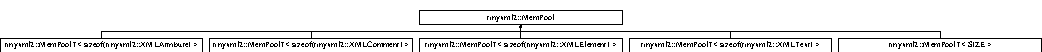
\includegraphics[height=0.691358cm]{classtinyxml2_1_1_mem_pool}
\end{center}
\end{figure}
\subsection*{Public Member Functions}
\begin{DoxyCompactItemize}
\item 
virtual int {\bfseries Item\+Size} () const  =0\hypertarget{classtinyxml2_1_1_mem_pool_afb3d8c6cbe91b44f90043d0d94dc7306}{}\label{classtinyxml2_1_1_mem_pool_afb3d8c6cbe91b44f90043d0d94dc7306}

\item 
virtual void $\ast$ {\bfseries Alloc} ()=0\hypertarget{classtinyxml2_1_1_mem_pool_a4f977b5fed752c0bbfe5295f469d6449}{}\label{classtinyxml2_1_1_mem_pool_a4f977b5fed752c0bbfe5295f469d6449}

\item 
virtual void {\bfseries Free} (void $\ast$)=0\hypertarget{classtinyxml2_1_1_mem_pool_a49e3bfac2cba2ebd6776b31e571f64f7}{}\label{classtinyxml2_1_1_mem_pool_a49e3bfac2cba2ebd6776b31e571f64f7}

\item 
virtual void {\bfseries Set\+Tracked} ()=0\hypertarget{classtinyxml2_1_1_mem_pool_ac5804dd1387b2e4de5eef710076a0db1}{}\label{classtinyxml2_1_1_mem_pool_ac5804dd1387b2e4de5eef710076a0db1}

\end{DoxyCompactItemize}


The documentation for this class was generated from the following file\+:\begin{DoxyCompactItemize}
\item 
Code/\+Reb\+Support/tinyxml2.\+h\end{DoxyCompactItemize}

\hypertarget{classtinyxml2_1_1_mem_pool_t}{}\section{tinyxml2\+:\+:Mem\+PoolT$<$ S\+I\+ZE $>$ Class Template Reference}
\label{classtinyxml2_1_1_mem_pool_t}\index{tinyxml2\+::\+Mem\+Pool\+T$<$ S\+I\+Z\+E $>$@{tinyxml2\+::\+Mem\+Pool\+T$<$ S\+I\+Z\+E $>$}}
Inheritance diagram for tinyxml2\+:\+:Mem\+PoolT$<$ S\+I\+ZE $>$\+:\begin{figure}[H]
\begin{center}
\leavevmode
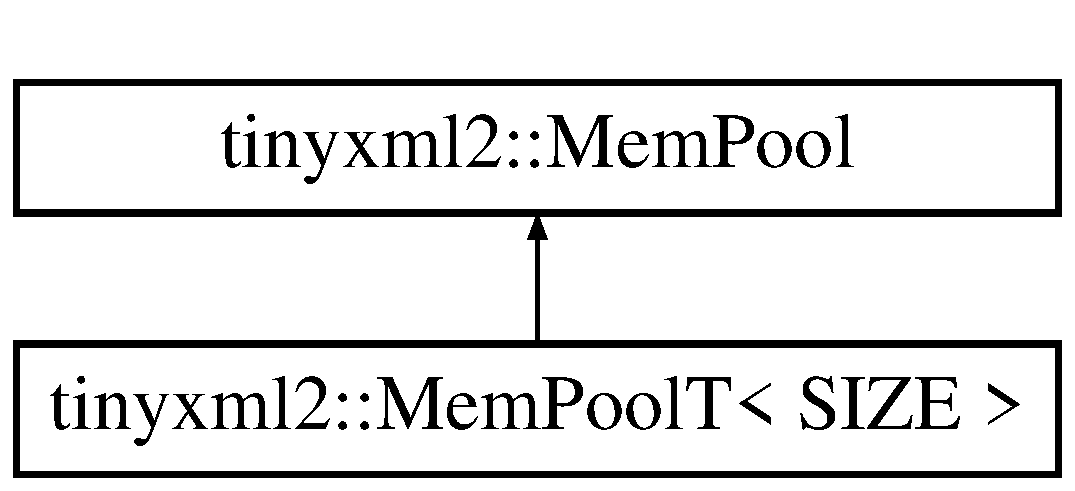
\includegraphics[height=2.000000cm]{classtinyxml2_1_1_mem_pool_t}
\end{center}
\end{figure}
\subsection*{Public Types}
\begin{DoxyCompactItemize}
\item 
enum \{ {\bfseries C\+O\+U\+NT} = (4$\ast$1024)/\+S\+I\+ZE
 \}\hypertarget{classtinyxml2_1_1_mem_pool_t_a04cf45156e6f913f93972869ff8a1d94}{}\label{classtinyxml2_1_1_mem_pool_t_a04cf45156e6f913f93972869ff8a1d94}

\end{DoxyCompactItemize}
\subsection*{Public Member Functions}
\begin{DoxyCompactItemize}
\item 
virtual int {\bfseries Item\+Size} () const \hypertarget{classtinyxml2_1_1_mem_pool_t_a7ec8778fe99f6e332615a703be0b48bc}{}\label{classtinyxml2_1_1_mem_pool_t_a7ec8778fe99f6e332615a703be0b48bc}

\item 
int {\bfseries Current\+Allocs} () const \hypertarget{classtinyxml2_1_1_mem_pool_t_a56be11b7db6a7ef00db17088a7769aab}{}\label{classtinyxml2_1_1_mem_pool_t_a56be11b7db6a7ef00db17088a7769aab}

\item 
virtual void $\ast$ {\bfseries Alloc} ()\hypertarget{classtinyxml2_1_1_mem_pool_t_aa9d785a48ffe6ea1be679bab13464486}{}\label{classtinyxml2_1_1_mem_pool_t_aa9d785a48ffe6ea1be679bab13464486}

\item 
virtual void {\bfseries Free} (void $\ast$mem)\hypertarget{classtinyxml2_1_1_mem_pool_t_a4f1a0c434e9e3d7391e5c16ed4ee8c70}{}\label{classtinyxml2_1_1_mem_pool_t_a4f1a0c434e9e3d7391e5c16ed4ee8c70}

\item 
void {\bfseries Trace} (const char $\ast$name)\hypertarget{classtinyxml2_1_1_mem_pool_t_a0bc596f271e0f139822c534238b3f244}{}\label{classtinyxml2_1_1_mem_pool_t_a0bc596f271e0f139822c534238b3f244}

\item 
void {\bfseries Set\+Tracked} ()\hypertarget{classtinyxml2_1_1_mem_pool_t_a7798932414916199a1bc0f9c3f368521}{}\label{classtinyxml2_1_1_mem_pool_t_a7798932414916199a1bc0f9c3f368521}

\item 
int {\bfseries Untracked} () const \hypertarget{classtinyxml2_1_1_mem_pool_t_a524b90d0edeac41964c06510757dce0f}{}\label{classtinyxml2_1_1_mem_pool_t_a524b90d0edeac41964c06510757dce0f}

\end{DoxyCompactItemize}


The documentation for this class was generated from the following file\+:\begin{DoxyCompactItemize}
\item 
Code/\+Reb\+Support/tinyxml2.\+h\end{DoxyCompactItemize}

\hypertarget{class_editor_1_1_open_g_l}{}\section{Editor.\+Open\+GL Class Reference}
\label{class_editor_1_1_open_g_l}\index{Editor.\+Open\+GL@{Editor.\+Open\+GL}}
\subsection*{Public Member Functions}
\begin{DoxyCompactItemize}
\item 
void {\bfseries CC} (Int\+Ptr hwnd)\hypertarget{class_editor_1_1_open_g_l_a8d3f6ea5e8944a3f0a6f62b66f8167af}{}\label{class_editor_1_1_open_g_l_a8d3f6ea5e8944a3f0a6f62b66f8167af}

\item 
void {\bfseries Render} ()\hypertarget{class_editor_1_1_open_g_l_a125f7fe6e9df02ef83d985e5d92f8936}{}\label{class_editor_1_1_open_g_l_a125f7fe6e9df02ef83d985e5d92f8936}

\end{DoxyCompactItemize}


The documentation for this class was generated from the following file\+:\begin{DoxyCompactItemize}
\item 
Code/\+Editor/Open\+G\+L.\+cs\end{DoxyCompactItemize}

\hypertarget{class_output}{}\section{Output Class Reference}
\label{class_output}\index{Output@{Output}}


The documentation for this class was generated from the following file\+:\begin{DoxyCompactItemize}
\item 
Code/\+Reb\+Game\+Logic/Reb\+Flow\+Graph.\+h\end{DoxyCompactItemize}

\hypertarget{structqt__meta__stringdata___editor__t}{}\section{qt\+\_\+meta\+\_\+stringdata\+\_\+\+Editor\+\_\+t Struct Reference}
\label{structqt__meta__stringdata___editor__t}\index{qt\+\_\+meta\+\_\+stringdata\+\_\+\+Editor\+\_\+t@{qt\+\_\+meta\+\_\+stringdata\+\_\+\+Editor\+\_\+t}}
\subsection*{Public Attributes}
\begin{DoxyCompactItemize}
\item 
Q\+Byte\+Array\+Data {\bfseries data} \mbox{[}1\mbox{]}\hypertarget{structqt__meta__stringdata___editor__t_ab6e6238a16780a51fa62204e031868fa}{}\label{structqt__meta__stringdata___editor__t_ab6e6238a16780a51fa62204e031868fa}

\item 
char {\bfseries stringdata} \mbox{[}7\mbox{]}\hypertarget{structqt__meta__stringdata___editor__t_a944fc81ee5a9ae7ee0a0f3b36afdaa40}{}\label{structqt__meta__stringdata___editor__t_a944fc81ee5a9ae7ee0a0f3b36afdaa40}

\end{DoxyCompactItemize}


The documentation for this struct was generated from the following file\+:\begin{DoxyCompactItemize}
\item 
Code/\+Editor/\+Generated\+Files/\+Debug/moc\+\_\+editor.\+cpp\end{DoxyCompactItemize}

\hypertarget{class_r_a_l_m_p}{}\section{R\+A\+L\+MP Class Reference}
\label{class_r_a_l_m_p}\index{R\+A\+L\+MP@{R\+A\+L\+MP}}


The documentation for this class was generated from the following file\+:\begin{DoxyCompactItemize}
\item 
Code/\+Reb\+Audio/Reb\+A\+L\+\_\+\+Music\+Player.\+h\end{DoxyCompactItemize}

\hypertarget{class_r_a_l_source}{}\section{R\+A\+L\+Source Class Reference}
\label{class_r_a_l_source}\index{R\+A\+L\+Source@{R\+A\+L\+Source}}
Inheritance diagram for R\+A\+L\+Source\+:\begin{figure}[H]
\begin{center}
\leavevmode
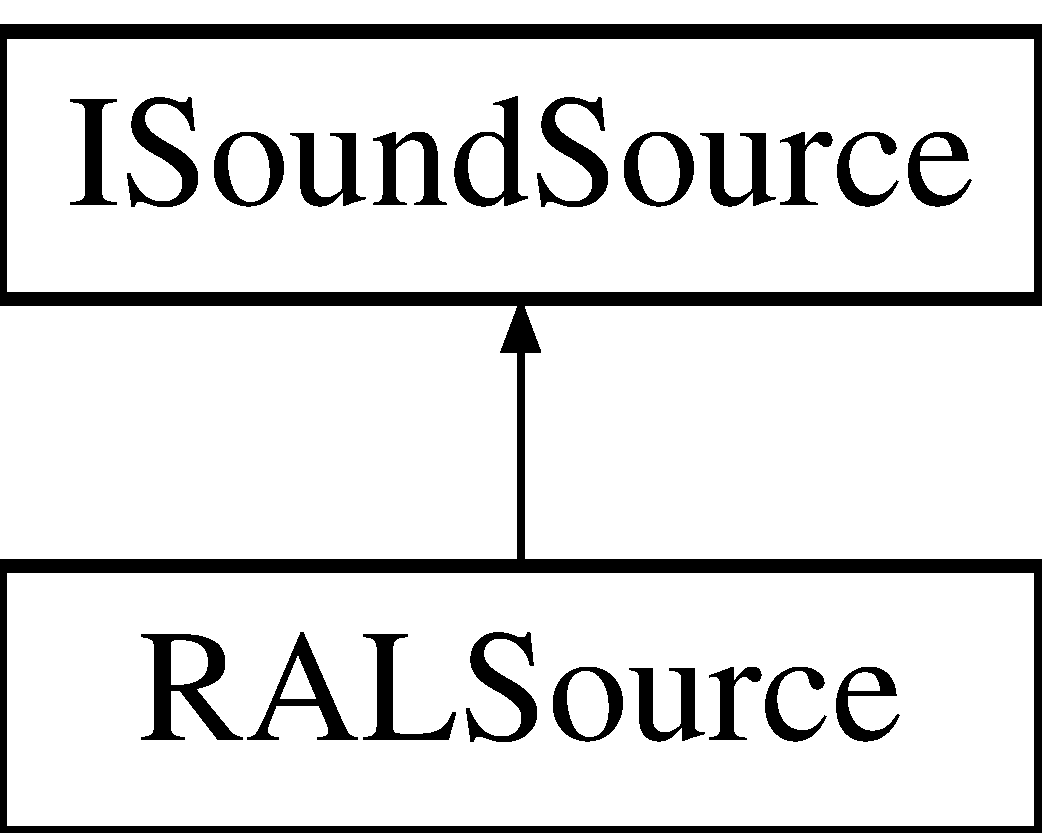
\includegraphics[height=2.000000cm]{class_r_a_l_source}
\end{center}
\end{figure}
\subsection*{Public Member Functions}
\begin{DoxyCompactItemize}
\item 
void {\bfseries Set\+Sound} ()\hypertarget{class_r_a_l_source_a550b6129730c0084f62db9c97fdc1a7d}{}\label{class_r_a_l_source_a550b6129730c0084f62db9c97fdc1a7d}

\item 
void {\bfseries Set\+Position} ()\hypertarget{class_r_a_l_source_ad251b7ddb84d9b747d3482d459549e52}{}\label{class_r_a_l_source_ad251b7ddb84d9b747d3482d459549e52}

\item 
void {\bfseries Play} ()\hypertarget{class_r_a_l_source_a6ba71af866c62209072d998b543ccdf5}{}\label{class_r_a_l_source_a6ba71af866c62209072d998b543ccdf5}

\item 
void {\bfseries Update} ()\hypertarget{class_r_a_l_source_a4a035de1d51ff72bb75957baeb0b98f8}{}\label{class_r_a_l_source_a4a035de1d51ff72bb75957baeb0b98f8}

\item 
void {\bfseries Stop} ()\hypertarget{class_r_a_l_source_a989d0d5cf2e00fc077c3ce5aa6da89af}{}\label{class_r_a_l_source_a989d0d5cf2e00fc077c3ce5aa6da89af}

\end{DoxyCompactItemize}


The documentation for this class was generated from the following files\+:\begin{DoxyCompactItemize}
\item 
Code/\+Reb\+Audio/Reb\+A\+L\+\_\+\+Sound\+Player.\+h\item 
Code/\+Reb\+Audio/Reb\+A\+L\+\_\+\+Sound\+Player.\+cpp\end{DoxyCompactItemize}

\hypertarget{struct_reb3_d___reb_matrix___c_struct}{}\section{Reb3\+D\+\_\+\+Reb\+Matrix\+\_\+\+C\+Struct Struct Reference}
\label{struct_reb3_d___reb_matrix___c_struct}\index{Reb3\+D\+\_\+\+Reb\+Matrix\+\_\+\+C\+Struct@{Reb3\+D\+\_\+\+Reb\+Matrix\+\_\+\+C\+Struct}}
\subsection*{Public Attributes}
\begin{DoxyCompactItemize}
\item 
Py\+Object\+\_\+\+H\+E\+AD Reb\+Matrix {\bfseries rm}\hypertarget{struct_reb3_d___reb_matrix___c_struct_a9607b320d258f3d1e388c139f0be3833}{}\label{struct_reb3_d___reb_matrix___c_struct_a9607b320d258f3d1e388c139f0be3833}

\end{DoxyCompactItemize}


The documentation for this struct was generated from the following file\+:\begin{DoxyCompactItemize}
\item 
Code/\+Reb\+Game\+Logic/\+R\+P\+S\+T\+L/R\+P\+M\+\_\+\+Reb3\+D.\+h\end{DoxyCompactItemize}

\hypertarget{struct_reb3_d___reb_vector___c_struct}{}\section{Reb3\+D\+\_\+\+Reb\+Vector\+\_\+\+C\+Struct Struct Reference}
\label{struct_reb3_d___reb_vector___c_struct}\index{Reb3\+D\+\_\+\+Reb\+Vector\+\_\+\+C\+Struct@{Reb3\+D\+\_\+\+Reb\+Vector\+\_\+\+C\+Struct}}
\subsection*{Public Attributes}
\begin{DoxyCompactItemize}
\item 
Py\+Object\+\_\+\+H\+E\+AD Reb\+Vector {\bfseries rv}\hypertarget{struct_reb3_d___reb_vector___c_struct_a37751ccfc25b985c2624fa841343395e}{}\label{struct_reb3_d___reb_vector___c_struct_a37751ccfc25b985c2624fa841343395e}

\end{DoxyCompactItemize}


The documentation for this struct was generated from the following file\+:\begin{DoxyCompactItemize}
\item 
Code/\+Reb\+Game\+Logic/\+R\+P\+S\+T\+L/R\+P\+M\+\_\+\+Reb3\+D.\+h\end{DoxyCompactItemize}

\hypertarget{class_reb_aabb}{}\section{Reb\+Aabb Class Reference}
\label{class_reb_aabb}\index{Reb\+Aabb@{Reb\+Aabb}}
\subsection*{Public Member Functions}
\begin{DoxyCompactItemize}
\item 
{\bfseries Reb\+Aabb} (Reb\+Vector vc\+Min, Reb\+Vector vc\+Max)\hypertarget{class_reb_aabb_adad0530f6ea18856446ada9a500046c8}{}\label{class_reb_aabb_adad0530f6ea18856446ada9a500046c8}

\item 
void {\bfseries Construct} (const \hyperlink{class_reb_obb}{Reb\+Obb} $\ast$p\+Obb)\hypertarget{class_reb_aabb_a842c0c11da33dcc252aaf7bfc08e5383}{}\label{class_reb_aabb_a842c0c11da33dcc252aaf7bfc08e5383}

\item 
int \hyperlink{class_reb_aabb_aa014c181038ba708fd3417302314cfef}{Cull} (const \hyperlink{class_reb_plane}{Reb\+Plane} $\ast$p\+Planes, int n\+Num\+Planes)
\item 
void {\bfseries Get\+Planes} (\hyperlink{class_reb_plane}{Reb\+Plane} $\ast$p\+Planes)\hypertarget{class_reb_aabb_a9c84f6459e1166c5756bf9dc206f40a5}{}\label{class_reb_aabb_a9c84f6459e1166c5756bf9dc206f40a5}

\item 
bool {\bfseries Contains} (const \hyperlink{class_reb_ray}{Reb\+Ray} \&Ray, float fL)\hypertarget{class_reb_aabb_a61bca793740fd05e25e3cb195a7518fb}{}\label{class_reb_aabb_a61bca793740fd05e25e3cb195a7518fb}

\item 
bool {\bfseries Intersects} (const \hyperlink{class_reb_ray}{Reb\+Ray} \&Ray, float $\ast$t)\hypertarget{class_reb_aabb_a1d6c74f5c62fef77121c9a829b389531}{}\label{class_reb_aabb_a1d6c74f5c62fef77121c9a829b389531}

\item 
bool {\bfseries Intersects} (const \hyperlink{class_reb_ray}{Reb\+Ray} \&Ray, float fL, float $\ast$t)\hypertarget{class_reb_aabb_ab09b2c44469e8107b5bfafab70bff413}{}\label{class_reb_aabb_ab09b2c44469e8107b5bfafab70bff413}

\item 
bool {\bfseries Intersects} (const \hyperlink{class_reb_aabb}{Reb\+Aabb} \&aabb)\hypertarget{class_reb_aabb_a9647aeefd17dadf7925468db4c84fb5a}{}\label{class_reb_aabb_a9647aeefd17dadf7925468db4c84fb5a}

\item 
bool {\bfseries Intersects} (const Reb\+Vector \&vc0)\hypertarget{class_reb_aabb_aa997b8a2529fd2478d62dcf63d3cb26f}{}\label{class_reb_aabb_aa997b8a2529fd2478d62dcf63d3cb26f}

\end{DoxyCompactItemize}
\subsection*{Public Attributes}
\begin{DoxyCompactItemize}
\item 
Reb\+Vector {\bfseries vc\+Min}\hypertarget{class_reb_aabb_afaaa4d04d02f4817e0a5546f037a174e}{}\label{class_reb_aabb_afaaa4d04d02f4817e0a5546f037a174e}

\item 
Reb\+Vector {\bfseries vc\+Max}\hypertarget{class_reb_aabb_a29ae6faad3eb6f11dac60ea699facc01}{}\label{class_reb_aabb_a29ae6faad3eb6f11dac60ea699facc01}

\item 
Reb\+Vector {\bfseries vc\+Center}\hypertarget{class_reb_aabb_ad1ee211287a1c77f6741442f7f07e837}{}\label{class_reb_aabb_ad1ee211287a1c77f6741442f7f07e837}

\end{DoxyCompactItemize}


\subsection{Member Function Documentation}
\index{Reb\+Aabb@{Reb\+Aabb}!Cull@{Cull}}
\index{Cull@{Cull}!Reb\+Aabb@{Reb\+Aabb}}
\subsubsection[{\texorpdfstring{Cull(const Reb\+Plane $\ast$p\+Planes, int n\+Num\+Planes)}{Cull(const RebPlane *pPlanes, int nNumPlanes)}}]{\setlength{\rightskip}{0pt plus 5cm}int Reb\+Aabb\+::\+Cull (
\begin{DoxyParamCaption}
\item[{const {\bf Reb\+Plane} $\ast$}]{p\+Planes, }
\item[{int}]{n\+Num\+Planes}
\end{DoxyParamCaption}
)}\hypertarget{class_reb_aabb_aa014c181038ba708fd3417302314cfef}{}\label{class_reb_aabb_aa014c181038ba708fd3417302314cfef}
Culls A\+A\+BB to n sided frustrum. Normals pointing outwards. -\/$>$ IN\+: \hyperlink{class_reb_plane}{Reb\+Plane} -\/ array of planes building frustrum int -\/ number of planes in array O\+UT\+: Reb\+V\+I\+S\+I\+B\+LE -\/ obb totally inside frustrum Reb\+C\+L\+I\+P\+P\+ED -\/ obb clipped by frustrum Reb\+C\+U\+L\+L\+ED -\/ obb totally outside frustrum 

The documentation for this class was generated from the following files\+:\begin{DoxyCompactItemize}
\item 
Code/\+Reb3\+D/Reb3d.\+h\item 
Code/\+Reb3\+D/Rebaabb.\+cpp\end{DoxyCompactItemize}

\hypertarget{class_reb_a_l}{}\section{Reb\+AL Class Reference}
\label{class_reb_a_l}\index{Reb\+AL@{Reb\+AL}}
Inheritance diagram for Reb\+AL\+:\begin{figure}[H]
\begin{center}
\leavevmode
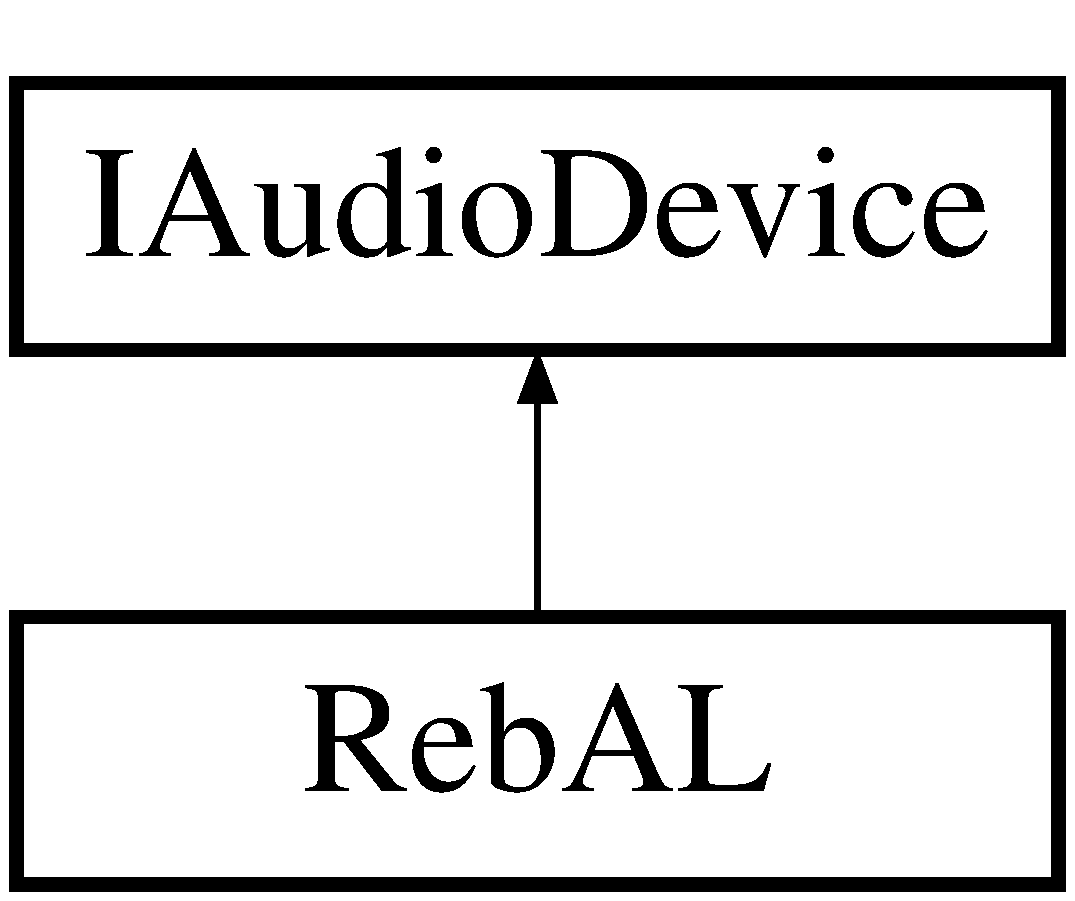
\includegraphics[height=2.000000cm]{class_reb_a_l}
\end{center}
\end{figure}
\subsection*{Public Member Functions}
\begin{DoxyCompactItemize}
\item 
void {\bfseries Init} ()\hypertarget{class_reb_a_l_a936a32d17119bc94bc4810fc26631815}{}\label{class_reb_a_l_a936a32d17119bc94bc4810fc26631815}

\item 
void {\bfseries Update} ()\hypertarget{class_reb_a_l_aa5a00fffbd0ca09b0bf6140ddfff87ee}{}\label{class_reb_a_l_aa5a00fffbd0ca09b0bf6140ddfff87ee}

\item 
void {\bfseries Release} ()\hypertarget{class_reb_a_l_ae65ac1ade00c6e8cc811d111b92523d3}{}\label{class_reb_a_l_ae65ac1ade00c6e8cc811d111b92523d3}

\item 
\hyperlink{class_i_music_player}{I\+Music\+Player} $\ast$ {\bfseries Get\+Music\+Player} ()\hypertarget{class_reb_a_l_a5913f825f76c75d5af96402399789e1d}{}\label{class_reb_a_l_a5913f825f76c75d5af96402399789e1d}

\item 
\hyperlink{class_i_sound_system}{I\+Sound\+System} $\ast$ {\bfseries Get\+Sound\+System} ()\hypertarget{class_reb_a_l_a4ac899ae49e9719b4adfae8c6464d699}{}\label{class_reb_a_l_a4ac899ae49e9719b4adfae8c6464d699}

\end{DoxyCompactItemize}


The documentation for this class was generated from the following files\+:\begin{DoxyCompactItemize}
\item 
Code/\+Reb\+Audio/Reb\+A\+L.\+h\item 
Code/\+Reb\+Audio/Reb\+A\+L.\+cpp\end{DoxyCompactItemize}

\hypertarget{class_reb_a_l_s_s}{}\section{Reb\+A\+L\+SS Class Reference}
\label{class_reb_a_l_s_s}\index{Reb\+A\+L\+SS@{Reb\+A\+L\+SS}}
Inheritance diagram for Reb\+A\+L\+SS\+:\begin{figure}[H]
\begin{center}
\leavevmode
\includegraphics[height=2.000000cm]{class_reb_a_l_s_s}
\end{center}
\end{figure}
\subsection*{Public Member Functions}
\begin{DoxyCompactItemize}
\item 
void {\bfseries Test} ()\hypertarget{class_reb_a_l_s_s_aa18aaf1660bf2c1b58b4bdd75b295a98}{}\label{class_reb_a_l_s_s_aa18aaf1660bf2c1b58b4bdd75b295a98}

\item 
void {\bfseries Update} ()\hypertarget{class_reb_a_l_s_s_a4f2b35c073e75d10a5d2d19ffc01d576}{}\label{class_reb_a_l_s_s_a4f2b35c073e75d10a5d2d19ffc01d576}

\end{DoxyCompactItemize}


The documentation for this class was generated from the following files\+:\begin{DoxyCompactItemize}
\item 
Code/\+Reb\+Audio/Reb\+A\+L\+\_\+\+Sound\+Player.\+h\item 
Code/\+Reb\+Audio/Reb\+A\+L\+\_\+\+Sound\+Player.\+cpp\end{DoxyCompactItemize}

\hypertarget{class_reb_decoder}{}\section{Reb\+Decoder Class Reference}
\label{class_reb_decoder}\index{Reb\+Decoder@{Reb\+Decoder}}
\subsection*{Public Member Functions}
\begin{DoxyCompactItemize}
\item 
void {\bfseries Load\+\_\+\+Wave\+\_\+\+File} (char $\ast$fname, unsigned int buff)\hypertarget{class_reb_decoder_a1bbe36c40cba91d0da261f016a26300d}{}\label{class_reb_decoder_a1bbe36c40cba91d0da261f016a26300d}

\item 
void {\bfseries Set\+Source} (std\+::string file)\hypertarget{class_reb_decoder_a9afc17a880a5fededbbaa6c90c1e05be}{}\label{class_reb_decoder_a9afc17a880a5fededbbaa6c90c1e05be}

\item 
void {\bfseries decode} (unsigned int buff, A\+Luint frequency=44100, A\+Lenum format=A\+L\+\_\+\+F\+O\+R\+M\+A\+T\+\_\+\+S\+T\+E\+R\+E\+O16)\hypertarget{class_reb_decoder_acddf0e5ad5b6f43cbd4de4553f091daa}{}\label{class_reb_decoder_acddf0e5ad5b6f43cbd4de4553f091daa}

\end{DoxyCompactItemize}
\subsection*{Public Attributes}
\begin{DoxyCompactItemize}
\item 
void $\ast$ {\bfseries testdata}\hypertarget{class_reb_decoder_a1bc0585c00154bf8afbf0f32a025795a}{}\label{class_reb_decoder_a1bc0585c00154bf8afbf0f32a025795a}

\end{DoxyCompactItemize}


The documentation for this class was generated from the following files\+:\begin{DoxyCompactItemize}
\item 
Code/\+Reb\+Audio/Reb\+F\+F\+Mpeg.\+h\item 
Code/\+Reb\+Audio/Reb\+F\+F\+Mpeg.\+cpp\end{DoxyCompactItemize}

\hypertarget{class_reb_dir}{}\section{Reb\+Dir Class Reference}
\label{class_reb_dir}\index{Reb\+Dir@{Reb\+Dir}}
\subsection*{Public Member Functions}
\begin{DoxyCompactItemize}
\item 
{\bfseries Reb\+Dir} (std\+::string abspath, \hyperlink{class_reb_dir}{Reb\+Dir} $\ast$spar=0)\hypertarget{class_reb_dir_af8d3ec742eeb3ec17bfb12e48884e025}{}\label{class_reb_dir_af8d3ec742eeb3ec17bfb12e48884e025}

\item 
std\+::string {\bfseries Get\+A\+Path} ()\hypertarget{class_reb_dir_a4e847c42a670ad41fb8e93f306f8ac00}{}\label{class_reb_dir_a4e847c42a670ad41fb8e93f306f8ac00}

\item 
std\+::string {\bfseries Get\+R\+Path} ()\hypertarget{class_reb_dir_a84e3c3c19b084bfd5cdba0f61f92d489}{}\label{class_reb_dir_a84e3c3c19b084bfd5cdba0f61f92d489}

\item 
std\+::string {\bfseries Get\+Name} ()\hypertarget{class_reb_dir_a1e34602e5b1e0f5aece2609c83b2c4c4}{}\label{class_reb_dir_a1e34602e5b1e0f5aece2609c83b2c4c4}

\item 
\hyperlink{class_reb_dir}{Reb\+Dir} $\ast$ {\bfseries Get\+Parent} ()\hypertarget{class_reb_dir_af9c0f3eacc112abecf0fbb5eefc82256}{}\label{class_reb_dir_af9c0f3eacc112abecf0fbb5eefc82256}

\item 
std\+::vector$<$ \hyperlink{class_reb_file}{Reb\+File} $\ast$ $>$ {\bfseries Search} (std\+::string name)\hypertarget{class_reb_dir_a1fa4025217b3f6decaf372fb9e55cc38}{}\label{class_reb_dir_a1fa4025217b3f6decaf372fb9e55cc38}

\item 
std\+::vector$<$ \hyperlink{class_reb_dir}{Reb\+Dir} $\ast$ $>$ {\bfseries Search\+Dir} (std\+::string name)\hypertarget{class_reb_dir_ab39ddb099bf247cfafc56f1a08c472ff}{}\label{class_reb_dir_ab39ddb099bf247cfafc56f1a08c472ff}

\item 
std\+::vector$<$ \hyperlink{class_reb_file}{Reb\+File} $\ast$ $>$ {\bfseries Get\+All\+Files} ()\hypertarget{class_reb_dir_a041db1c6010708c0c892265224497c33}{}\label{class_reb_dir_a041db1c6010708c0c892265224497c33}

\item 
std\+::vector$<$ \hyperlink{class_reb_dir}{Reb\+Dir} $\ast$ $>$ $\ast$ {\bfseries Get\+Dirs} ()\hypertarget{class_reb_dir_a77594fb772172918a412990a3e556bca}{}\label{class_reb_dir_a77594fb772172918a412990a3e556bca}

\item 
std\+::vector$<$ \hyperlink{class_reb_file}{Reb\+File} $\ast$ $>$ $\ast$ {\bfseries Get\+Files} ()\hypertarget{class_reb_dir_a123b46a26d2500e362edaa38d6b2c652}{}\label{class_reb_dir_a123b46a26d2500e362edaa38d6b2c652}

\end{DoxyCompactItemize}


The documentation for this class was generated from the following files\+:\begin{DoxyCompactItemize}
\item 
Code/\+Reb\+Support/Reb\+File\+System.\+h\item 
Code/\+Reb\+Support/Reb\+File\+System.\+cpp\end{DoxyCompactItemize}

\hypertarget{class_reb_entity}{}\section{Reb\+Entity Class Reference}
\label{class_reb_entity}\index{Reb\+Entity@{Reb\+Entity}}
\subsection*{Public Member Functions}
\begin{DoxyCompactItemize}
\item 
{\bfseries Reb\+Entity} (\hyperlink{class_reb_file}{Reb\+File} $\ast$sf, std\+::string name, Reb\+Vector spos=Reb\+Vector(0, 0, 0), std\+::map$<$ std\+::string, std\+::string $>$ $\ast$initlist=0)\hypertarget{class_reb_entity_a20bf721e729214ef43b8e99d1efbba55}{}\label{class_reb_entity_a20bf721e729214ef43b8e99d1efbba55}

\item 
void {\bfseries Set\+Pos} (Reb\+Vector spos)\hypertarget{class_reb_entity_ab1512f8c9894fdc03b7cec53d1d2660b}{}\label{class_reb_entity_ab1512f8c9894fdc03b7cec53d1d2660b}

\item 
void {\bfseries Set\+Param} (std\+::string key, std\+::string value)\hypertarget{class_reb_entity_a17c456928d4f201c550a6873c24d868c}{}\label{class_reb_entity_a17c456928d4f201c550a6873c24d868c}

\item 
void {\bfseries Update} ()\hypertarget{class_reb_entity_af496e1efac2571e4664f34e143924e2b}{}\label{class_reb_entity_af496e1efac2571e4664f34e143924e2b}

\item 
Reb\+Vector {\bfseries Get\+Pos} ()\hypertarget{class_reb_entity_a063f4b44ded0e413ac665cd847f8c4df}{}\label{class_reb_entity_a063f4b44ded0e413ac665cd847f8c4df}

\item 
std\+::string {\bfseries Get\+Param} (std\+::string key)\hypertarget{class_reb_entity_ae1b1310baf5c6e6bb4adbc98862ec93d}{}\label{class_reb_entity_ae1b1310baf5c6e6bb4adbc98862ec93d}

\end{DoxyCompactItemize}


The documentation for this class was generated from the following files\+:\begin{DoxyCompactItemize}
\item 
Code/\+Reb\+Entity\+System/Reb\+Entity.\+h\item 
Code/\+Reb\+Entity\+System/Reb\+Entity.\+cpp\end{DoxyCompactItemize}

\hypertarget{class_reb_entity_system}{}\section{Reb\+Entity\+System Class Reference}
\label{class_reb_entity_system}\index{Reb\+Entity\+System@{Reb\+Entity\+System}}
\subsection*{Public Member Functions}
\begin{DoxyCompactItemize}
\item 
{\bfseries Reb\+Entity\+System} (\hyperlink{class_reb_g_d_c}{Reb\+G\+DC} $\ast$sgd)\hypertarget{class_reb_entity_system_aa32a0be87f9d69e72eb108a7de8e65c9}{}\label{class_reb_entity_system_aa32a0be87f9d69e72eb108a7de8e65c9}

\item 
\hyperlink{class_reb_entity}{Reb\+Entity} $\ast$ {\bfseries Create\+Entity} (std\+::string type, std\+::string name)\hypertarget{class_reb_entity_system_a9a3164b43c924ce1f98da2c3db2e6293}{}\label{class_reb_entity_system_a9a3164b43c924ce1f98da2c3db2e6293}

\item 
\hyperlink{class_reb_entity}{Reb\+Entity} $\ast$ {\bfseries Get\+By\+Name} (std\+::string name)\hypertarget{class_reb_entity_system_af29cbbb2176b4250767e0919b3cf5af1}{}\label{class_reb_entity_system_af29cbbb2176b4250767e0919b3cf5af1}

\item 
void {\bfseries Delete\+Entity} (\hyperlink{class_reb_entity}{Reb\+Entity} $\ast$todel)\hypertarget{class_reb_entity_system_ace78e2f071ec0c8d31fa1ed31e740a0f}{}\label{class_reb_entity_system_ace78e2f071ec0c8d31fa1ed31e740a0f}

\item 
void {\bfseries Update\+All} ()\hypertarget{class_reb_entity_system_a9fdc56228b5c2a446c1a387a8739737d}{}\label{class_reb_entity_system_a9fdc56228b5c2a446c1a387a8739737d}

\end{DoxyCompactItemize}


The documentation for this class was generated from the following files\+:\begin{DoxyCompactItemize}
\item 
Code/\+Reb\+Entity\+System/Reb\+Entity\+System.\+h\item 
Code/\+Reb\+Entity\+System/Reb\+Entity\+System.\+cpp\end{DoxyCompactItemize}

\hypertarget{class_reb_env}{}\section{Reb\+Env Class Reference}
\label{class_reb_env}\index{Reb\+Env@{Reb\+Env}}
Inheritance diagram for Reb\+Env\+:\begin{figure}[H]
\begin{center}
\leavevmode
\includegraphics[height=2.000000cm]{class_reb_env}
\end{center}
\end{figure}
\subsection*{Public Member Functions}
\begin{DoxyCompactItemize}
\item 
\hyperlink{class_i_terrain}{I\+Terrain} $\ast$ {\bfseries Create\+Terrain} ()\hypertarget{class_reb_env_a3748a218a3f1423a5f41353ae32bfed7}{}\label{class_reb_env_a3748a218a3f1423a5f41353ae32bfed7}

\item 
\hyperlink{class_i_terrain}{I\+Terrain} $\ast$ {\bfseries Create\+Terrain} (std\+::string hmf)\hypertarget{class_reb_env_ab082c1fcb061d9b6dfd4d67a5156874e}{}\label{class_reb_env_ab082c1fcb061d9b6dfd4d67a5156874e}

\item 
std\+::vector$<$ \hyperlink{class_i_terrain}{I\+Terrain} $\ast$ $>$ $\ast$ {\bfseries Get\+Terrains} ()\hypertarget{class_reb_env_abb92f4b2aab9d000ddcb74b7cf8470ea}{}\label{class_reb_env_abb92f4b2aab9d000ddcb74b7cf8470ea}

\item 
void {\bfseries Delete\+Terrain} (\hyperlink{class_i_terrain}{I\+Terrain} $\ast$del)\hypertarget{class_reb_env_a26d45064c84264785a2b7b7e993dc858}{}\label{class_reb_env_a26d45064c84264785a2b7b7e993dc858}

\end{DoxyCompactItemize}


The documentation for this class was generated from the following files\+:\begin{DoxyCompactItemize}
\item 
Code/\+Reb\+G\+L/Reb\+Env.\+h\item 
Code/\+Reb\+G\+L/Reb\+Env.\+cpp\end{DoxyCompactItemize}

\hypertarget{union_reb_event}{}\section{Reb\+Event Union Reference}
\label{union_reb_event}\index{Reb\+Event@{Reb\+Event}}
\subsection*{Public Attributes}
\begin{DoxyCompactItemize}
\item 
Event\+Type {\bfseries Type}\hypertarget{union_reb_event_a24ad77f260f8932a452888a1b56dd7bc}{}\label{union_reb_event_a24ad77f260f8932a452888a1b56dd7bc}

\item 
\hyperlink{struct_reb_quit_event}{Reb\+Quit\+Event} {\bfseries quit}\hypertarget{union_reb_event_aa0204985fc02b6993be96a66fcda4310}{}\label{union_reb_event_aa0204985fc02b6993be96a66fcda4310}

\item 
\hyperlink{struct_reb_mouse_motion_event}{Reb\+Mouse\+Motion\+Event} {\bfseries mousemot}\hypertarget{union_reb_event_a8555acd147ae2690ad1ac3d5662d073d}{}\label{union_reb_event_a8555acd147ae2690ad1ac3d5662d073d}

\item 
\hyperlink{struct_reb_mouse_key_event}{Reb\+Mouse\+Key\+Event} {\bfseries mousekey}\hypertarget{union_reb_event_a7999eaa3e4f3f73c4ca3d0933426f2dd}{}\label{union_reb_event_a7999eaa3e4f3f73c4ca3d0933426f2dd}

\item 
\hyperlink{struct_reb_user_event}{Reb\+User\+Event} {\bfseries user}\hypertarget{union_reb_event_a1c5d61209fd44b0b4432a741ecba4934}{}\label{union_reb_event_a1c5d61209fd44b0b4432a741ecba4934}

\item 
\hyperlink{class_reb_key_event}{Reb\+Key\+Event} {\bfseries key}\hypertarget{union_reb_event_a6cb945d219768cc8bf4f154e5ec8264b}{}\label{union_reb_event_a6cb945d219768cc8bf4f154e5ec8264b}

\item 
unsigned int {\bfseries compid}\hypertarget{union_reb_event_a01ca4d8c3ebebd777a7c49a221a8dd4b}{}\label{union_reb_event_a01ca4d8c3ebebd777a7c49a221a8dd4b}

\end{DoxyCompactItemize}


The documentation for this union was generated from the following file\+:\begin{DoxyCompactItemize}
\item 
Code/\+Reb\+Window/Event\+Struct.\+h\end{DoxyCompactItemize}

\hypertarget{class_reb_file}{}\section{Reb\+File Class Reference}
\label{class_reb_file}\index{Reb\+File@{Reb\+File}}
\subsection*{Public Member Functions}
\begin{DoxyCompactItemize}
\item 
{\bfseries Reb\+File} (std\+::string abspath, \hyperlink{class_reb_dir}{Reb\+Dir} $\ast$spar=0)\hypertarget{class_reb_file_a1f008b4a15ba4196acf03dc033003f83}{}\label{class_reb_file_a1f008b4a15ba4196acf03dc033003f83}

\item 
std\+::string {\bfseries Get\+Name} (bool wex=true)\hypertarget{class_reb_file_a1815f620a75028b52aec4751c7440c0f}{}\label{class_reb_file_a1815f620a75028b52aec4751c7440c0f}

\item 
std\+::string {\bfseries Get\+A\+Path} ()\hypertarget{class_reb_file_a15725b9679f08f3880370c149acf4f5a}{}\label{class_reb_file_a15725b9679f08f3880370c149acf4f5a}

\item 
std\+::string {\bfseries Get\+R\+Path} ()\hypertarget{class_reb_file_a249ac0c209407717c9f3650d9dfe08c8}{}\label{class_reb_file_a249ac0c209407717c9f3650d9dfe08c8}

\item 
std\+::string {\bfseries Get\+Extension} ()\hypertarget{class_reb_file_ad3dfa51debbbe1421bd4b29ba769d883}{}\label{class_reb_file_ad3dfa51debbbe1421bd4b29ba769d883}

\item 
\hyperlink{class_reb_dir}{Reb\+Dir} $\ast$ {\bfseries Get\+Parent} ()\hypertarget{class_reb_file_a5a035c1d22c88c4d00edf89a723c7d64}{}\label{class_reb_file_a5a035c1d22c88c4d00edf89a723c7d64}

\end{DoxyCompactItemize}


The documentation for this class was generated from the following files\+:\begin{DoxyCompactItemize}
\item 
Code/\+Reb\+Support/Reb\+File\+System.\+h\item 
Code/\+Reb\+Support/Reb\+File\+System.\+cpp\end{DoxyCompactItemize}

\hypertarget{class_reb_file_system}{}\section{Reb\+File\+System Class Reference}
\label{class_reb_file_system}\index{Reb\+File\+System@{Reb\+File\+System}}
\subsection*{Public Member Functions}
\begin{DoxyCompactItemize}
\item 
std\+::vector$<$ \hyperlink{class_reb_file}{Reb\+File} $\ast$ $>$ {\bfseries Search} (std\+::string name)\hypertarget{class_reb_file_system_af0ea3d08f0799e3fe8e01d2d4ff2b09a}{}\label{class_reb_file_system_af0ea3d08f0799e3fe8e01d2d4ff2b09a}

\item 
std\+::vector$<$ \hyperlink{class_reb_dir}{Reb\+Dir} $\ast$ $>$ {\bfseries Search\+Dir} (std\+::string name)\hypertarget{class_reb_file_system_a3fdfa32965fc99bd3c7e0b6b4c9ebc61}{}\label{class_reb_file_system_a3fdfa32965fc99bd3c7e0b6b4c9ebc61}

\item 
std\+::vector$<$ \hyperlink{class_reb_file}{Reb\+File} $\ast$ $>$ {\bfseries Get\+All\+Files} ()\hypertarget{class_reb_file_system_ab14ac333e7571313c71f6dc6c5783f9e}{}\label{class_reb_file_system_ab14ac333e7571313c71f6dc6c5783f9e}

\end{DoxyCompactItemize}


The documentation for this class was generated from the following files\+:\begin{DoxyCompactItemize}
\item 
Code/\+Reb\+Support/Reb\+File\+System.\+h\item 
Code/\+Reb\+Support/Reb\+File\+System.\+cpp\end{DoxyCompactItemize}

\hypertarget{class_reb_flow_graph}{}\section{Reb\+Flow\+Graph Class Reference}
\label{class_reb_flow_graph}\index{Reb\+Flow\+Graph@{Reb\+Flow\+Graph}}


The documentation for this class was generated from the following file\+:\begin{DoxyCompactItemize}
\item 
Code/\+Reb\+Game\+Logic/Reb\+Flow\+Graph.\+h\end{DoxyCompactItemize}

\hypertarget{class_reb_flow_node}{}\section{Reb\+Flow\+Node Class Reference}
\label{class_reb_flow_node}\index{Reb\+Flow\+Node@{Reb\+Flow\+Node}}


The documentation for this class was generated from the following file\+:\begin{DoxyCompactItemize}
\item 
Code/\+Reb\+Game\+Logic/Reb\+Flow\+Graph.\+h\end{DoxyCompactItemize}

\hypertarget{class_reb_game}{}\section{Reb\+Game Class Reference}
\label{class_reb_game}\index{Reb\+Game@{Reb\+Game}}
Inheritance diagram for Reb\+Game\+:\begin{figure}[H]
\begin{center}
\leavevmode
\includegraphics[height=2.000000cm]{class_reb_game}
\end{center}
\end{figure}
\subsection*{Public Member Functions}
\begin{DoxyCompactItemize}
\item 
void {\bfseries Init} ()\hypertarget{class_reb_game_a1981bc8d7452e3064c0d4024a7651e0d}{}\label{class_reb_game_a1981bc8d7452e3064c0d4024a7651e0d}

\item 
void {\bfseries Game\+Loop} ()\hypertarget{class_reb_game_a38d3fb9bd1c949bf5ea9879c1f4f218f}{}\label{class_reb_game_a38d3fb9bd1c949bf5ea9879c1f4f218f}

\item 
void \hyperlink{class_reb_game_acf2c9d06a2a5206868f7f3c592768e70}{Release} ()
\end{DoxyCompactItemize}
\subsection*{Public Attributes}
\begin{DoxyCompactItemize}
\item 
\hyperlink{class_reb_file_system}{Reb\+File\+System} $\ast$ {\bfseries rfs}\hypertarget{class_reb_game_a83286fd9595aa8d8e55db8520b7f5798}{}\label{class_reb_game_a83286fd9595aa8d8e55db8520b7f5798}

\item 
\hyperlink{class_reb_timer}{Reb\+Timer} {\bfseries rtimer}\hypertarget{class_reb_game_abdecc4fa3befe4a367879eb1524b687d}{}\label{class_reb_game_abdecc4fa3befe4a367879eb1524b687d}

\end{DoxyCompactItemize}


\subsection{Member Function Documentation}
\index{Reb\+Game@{Reb\+Game}!Release@{Release}}
\index{Release@{Release}!Reb\+Game@{Reb\+Game}}
\subsubsection[{\texorpdfstring{Release()}{Release()}}]{\setlength{\rightskip}{0pt plus 5cm}void Reb\+Game\+::\+Release (
\begin{DoxyParamCaption}
{}
\end{DoxyParamCaption}
)\hspace{0.3cm}{\ttfamily [virtual]}}\hypertarget{class_reb_game_acf2c9d06a2a5206868f7f3c592768e70}{}\label{class_reb_game_acf2c9d06a2a5206868f7f3c592768e70}
{\itshape ras.\+Get\+Audio\+Device()-\/$>$Get\+Music\+Player()-\/$>$Stop();}/ 

Implements \hyperlink{class_i_game}{I\+Game}.



The documentation for this class was generated from the following files\+:\begin{DoxyCompactItemize}
\item 
Code/\+Reb\+Game/Reb\+Game.\+h\item 
Code/\+Reb\+Game/Reb\+Game.\+cpp\end{DoxyCompactItemize}

\hypertarget{class_reb_game_logic}{}\section{Reb\+Game\+Logic Class Reference}
\label{class_reb_game_logic}\index{Reb\+Game\+Logic@{Reb\+Game\+Logic}}
Inheritance diagram for Reb\+Game\+Logic\+:\begin{figure}[H]
\begin{center}
\leavevmode
\includegraphics[height=2.000000cm]{class_reb_game_logic}
\end{center}
\end{figure}
\subsection*{Public Member Functions}
\begin{DoxyCompactItemize}
\item 
{\bfseries Reb\+Game\+Logic} (\hyperlink{class_reb_g_d_c}{Reb\+G\+DC} $\ast$set)\hypertarget{class_reb_game_logic_a46b612f497f76e0a200db59bea1ee89d}{}\label{class_reb_game_logic_a46b612f497f76e0a200db59bea1ee89d}

\item 
\hyperlink{class_i_script_manager}{I\+Script\+Manager} $\ast$ {\bfseries Get\+I\+SM} ()\hypertarget{class_reb_game_logic_a939ddfc5e0b54f20168796b2a94aa891}{}\label{class_reb_game_logic_a939ddfc5e0b54f20168796b2a94aa891}

\end{DoxyCompactItemize}


The documentation for this class was generated from the following files\+:\begin{DoxyCompactItemize}
\item 
Code/\+Reb\+Game\+Logic/Reb\+Game\+Logic.\+h\item 
Code/\+Reb\+Game\+Logic/Reb\+Game\+Logic.\+cpp\end{DoxyCompactItemize}

\hypertarget{class_reb_g_buffer}{}\section{Reb\+G\+Buffer Class Reference}
\label{class_reb_g_buffer}\index{Reb\+G\+Buffer@{Reb\+G\+Buffer}}
\subsection*{Public Member Functions}
\begin{DoxyCompactItemize}
\item 
void {\bfseries Write} ()\hypertarget{class_reb_g_buffer_a860a14f1c082f5d87b361b22fd980e98}{}\label{class_reb_g_buffer_a860a14f1c082f5d87b361b22fd980e98}

\item 
void {\bfseries bind} (G\+Luint handle)\hypertarget{class_reb_g_buffer_af23826c93bf94accba77f0be29d53e33}{}\label{class_reb_g_buffer_af23826c93bf94accba77f0be29d53e33}

\item 
int {\bfseries Get\+Postex} ()\hypertarget{class_reb_g_buffer_a4fd1472dd306fc4ed8479e144f117a3f}{}\label{class_reb_g_buffer_a4fd1472dd306fc4ed8479e144f117a3f}

\item 
void {\bfseries Read} ()\hypertarget{class_reb_g_buffer_afb591d9daa20fa0a6e139b4a60f446a3}{}\label{class_reb_g_buffer_afb591d9daa20fa0a6e139b4a60f446a3}

\item 
{\bfseries R\+TT} ()\hypertarget{class_reb_g_buffer_adb1f55f86701d3b5b353def05ba32aad}{}\label{class_reb_g_buffer_adb1f55f86701d3b5b353def05ba32aad}

\item 
void {\bfseries Write} ()\hypertarget{class_reb_g_buffer_a860a14f1c082f5d87b361b22fd980e98}{}\label{class_reb_g_buffer_a860a14f1c082f5d87b361b22fd980e98}

\item 
void {\bfseries bind} (G\+Luint handle)\hypertarget{class_reb_g_buffer_af23826c93bf94accba77f0be29d53e33}{}\label{class_reb_g_buffer_af23826c93bf94accba77f0be29d53e33}

\item 
int {\bfseries Get\+Postex} ()\hypertarget{class_reb_g_buffer_a4fd1472dd306fc4ed8479e144f117a3f}{}\label{class_reb_g_buffer_a4fd1472dd306fc4ed8479e144f117a3f}

\item 
void {\bfseries Read} ()\hypertarget{class_reb_g_buffer_afb591d9daa20fa0a6e139b4a60f446a3}{}\label{class_reb_g_buffer_afb591d9daa20fa0a6e139b4a60f446a3}

\end{DoxyCompactItemize}


The documentation for this class was generated from the following files\+:\begin{DoxyCompactItemize}
\item 
Code/\+Reb\+G\+L/Reb\+G\+L\+\_\+\+Graphic\+Utilities.\+h\item 
Code/\+Reb\+G\+L/Reb\+G\+L\+\_\+\+Render\+Helpers.\+h\item 
Code/\+Reb\+G\+L/Reb\+G\+L\+\_\+\+Graphic\+Utilities.\+cpp\end{DoxyCompactItemize}

\hypertarget{class_reb_g_d_c}{}\section{Reb\+G\+DC Class Reference}
\label{class_reb_g_d_c}\index{Reb\+G\+DC@{Reb\+G\+DC}}
\subsection*{Public Attributes}
\begin{DoxyCompactItemize}
\item 
\hyperlink{class_i_w_a_e_m}{I\+W\+A\+EM} $\ast$ {\bfseries waem}\hypertarget{class_reb_g_d_c_a839485e984af193e81d6dcc5e40223c9}{}\label{class_reb_g_d_c_a839485e984af193e81d6dcc5e40223c9}

\item 
\hyperlink{class_i_render_device}{I\+Render\+Device} $\ast$ {\bfseries rd}\hypertarget{class_reb_g_d_c_af25180fbb5b4440d8758369f3ca21264}{}\label{class_reb_g_d_c_af25180fbb5b4440d8758369f3ca21264}

\item 
\hyperlink{class_reb_game_logic}{Reb\+Game\+Logic} $\ast$ {\bfseries rlogic}\hypertarget{class_reb_g_d_c_a1b4baea32b6dae4d7ce62b5f5097ccda}{}\label{class_reb_g_d_c_a1b4baea32b6dae4d7ce62b5f5097ccda}

\item 
\hyperlink{class_i_window}{I\+Window} $\ast$ {\bfseries window}\hypertarget{class_reb_g_d_c_ae5570dfbb9cb688315bf7f532642feb2}{}\label{class_reb_g_d_c_ae5570dfbb9cb688315bf7f532642feb2}

\item 
bool {\bfseries grp}\hypertarget{class_reb_g_d_c_a0c468883aef503f6e9f8cd9697ae7992}{}\label{class_reb_g_d_c_a0c468883aef503f6e9f8cd9697ae7992}

\item 
\hyperlink{class_reb_file_system}{Reb\+File\+System} $\ast$ {\bfseries rfs}\hypertarget{class_reb_g_d_c_a9613fa4261400a3fff835de56b8b2116}{}\label{class_reb_g_d_c_a9613fa4261400a3fff835de56b8b2116}

\end{DoxyCompactItemize}


The documentation for this class was generated from the following file\+:\begin{DoxyCompactItemize}
\item 
Code/\+Reb\+Support/Reb\+G\+D\+C.\+h\end{DoxyCompactItemize}

\hypertarget{class_reb_g_l}{}\section{Reb\+GL Class Reference}
\label{class_reb_g_l}\index{Reb\+GL@{Reb\+GL}}
Inheritance diagram for Reb\+GL\+:\begin{figure}[H]
\begin{center}
\leavevmode
\includegraphics[height=2.000000cm]{class_reb_g_l}
\end{center}
\end{figure}
\subsection*{Public Member Functions}
\begin{DoxyCompactItemize}
\item 
{\bfseries Reb\+GL} (\hyperlink{class_reb_g_d_c}{Reb\+G\+DC} $\ast$gdc)\hypertarget{class_reb_g_l_a1299f244c431d291797af293f8cadc72}{}\label{class_reb_g_l_a1299f244c431d291797af293f8cadc72}

\item 
void {\bfseries Set\+Resolution} (unsigned int w, unsigned int h)\hypertarget{class_reb_g_l_aff84b4e00dee30286513a4bdd1d0e728}{}\label{class_reb_g_l_aff84b4e00dee30286513a4bdd1d0e728}

\item 
void {\bfseries Clear\+Color} (float r, float g, float b, float a)\hypertarget{class_reb_g_l_a88abd24ddf39cf6a88e904a262fe96aa}{}\label{class_reb_g_l_a88abd24ddf39cf6a88e904a262fe96aa}

\item 
void {\bfseries Start\+Draw} (Methold met)\hypertarget{class_reb_g_l_ac41a4e102588d6d11c1ac1cd679ab1f5}{}\label{class_reb_g_l_ac41a4e102588d6d11c1ac1cd679ab1f5}

\item 
void {\bfseries Vertex3} (float x, float y, float z)\hypertarget{class_reb_g_l_a57e7e9268558c9c9490dc8526ee38ec1}{}\label{class_reb_g_l_a57e7e9268558c9c9490dc8526ee38ec1}

\item 
void {\bfseries Vertex3} (Reb\+Vector RV)\hypertarget{class_reb_g_l_a79439bd8604df7dead9858e53a08f627}{}\label{class_reb_g_l_a79439bd8604df7dead9858e53a08f627}

\item 
void {\bfseries Normal} (Reb\+Vector RV)\hypertarget{class_reb_g_l_a97d64fb61e1a465ce0e1d85685f889f7}{}\label{class_reb_g_l_a97d64fb61e1a465ce0e1d85685f889f7}

\item 
void {\bfseries Material\+Setup} (\hyperlink{class_reb_material}{Reb\+Material} rm)\hypertarget{class_reb_g_l_a9386392d17167a9ec682dbcf18d7356d}{}\label{class_reb_g_l_a9386392d17167a9ec682dbcf18d7356d}

\item 
void {\bfseries Text\+Coord2} (float s, float t)\hypertarget{class_reb_g_l_a22796f0c3d9281456a509847fcd945f9}{}\label{class_reb_g_l_a22796f0c3d9281456a509847fcd945f9}

\item 
void {\bfseries Bind\+Texture} (U\+I\+NT id)\hypertarget{class_reb_g_l_a0fab00acb6978968603dd5f567f51917}{}\label{class_reb_g_l_a0fab00acb6978968603dd5f567f51917}

\item 
void {\bfseries Color} (float r, float g, float b)\hypertarget{class_reb_g_l_aa84d7b69e407faa7488887a9329bb9c7}{}\label{class_reb_g_l_aa84d7b69e407faa7488887a9329bb9c7}

\item 
void {\bfseries End\+Draw} ()\hypertarget{class_reb_g_l_aa1f59fc89eaad11a311c77969e38f538}{}\label{class_reb_g_l_aa1f59fc89eaad11a311c77969e38f538}

\item 
Reb\+Matrix {\bfseries Get\+Viewport\+Mat} ()\hypertarget{class_reb_g_l_a926d3465d00d67e5d1229ff3cca22ee5}{}\label{class_reb_g_l_a926d3465d00d67e5d1229ff3cca22ee5}

\item 
void {\bfseries Set\+Viewport\+Mat} (Reb\+Matrix svm)\hypertarget{class_reb_g_l_a72a4a10017e0e719ddebe2f39fcb589c}{}\label{class_reb_g_l_a72a4a10017e0e719ddebe2f39fcb589c}

\item 
void $\ast$$\ast$ {\bfseries Get\+Viewport\+ID} ()\hypertarget{class_reb_g_l_a10b62dc3d65d9167ef10f5f1423d0fd8}{}\label{class_reb_g_l_a10b62dc3d65d9167ef10f5f1423d0fd8}

\item 
void {\bfseries Get\+Viewport\+Size} (unsigned int $\ast$w, unsigned int $\ast$h)\hypertarget{class_reb_g_l_a0f05955070e51f2f47242c9bb8aa847b}{}\label{class_reb_g_l_a0f05955070e51f2f47242c9bb8aa847b}

\item 
\hyperlink{class_i_skin_manager}{I\+Skin\+Manager} $\ast$ {\bfseries Get\+Skin\+Manager} ()\hypertarget{class_reb_g_l_ade78ba9aa97586f1608d0986120c4f40}{}\label{class_reb_g_l_ade78ba9aa97586f1608d0986120c4f40}

\item 
\hyperlink{class_i_vertex_cache_manager}{I\+Vertex\+Cache\+Manager} $\ast$ {\bfseries Get\+Vertex\+Cache\+Manager} ()\hypertarget{class_reb_g_l_a7442199d1dc6762083f7af38f5c9481b}{}\label{class_reb_g_l_a7442199d1dc6762083f7af38f5c9481b}

\item 
\hyperlink{class_i_game_env}{I\+Game\+Env} $\ast$ {\bfseries Get\+Env} ()\hypertarget{class_reb_g_l_acfc702ba1f9eb20a6c97ca72eee1a1a3}{}\label{class_reb_g_l_acfc702ba1f9eb20a6c97ca72eee1a1a3}

\item 
\hyperlink{class_i_light_system}{I\+Light\+System} $\ast$ {\bfseries Get\+Light\+System} ()\hypertarget{class_reb_g_l_a57557a3c7812b927ad00b3a7ed0544b3}{}\label{class_reb_g_l_a57557a3c7812b927ad00b3a7ed0544b3}

\item 
void {\bfseries Swap} (void $\ast$window)\hypertarget{class_reb_g_l_a314341db9e01ae7524be31cbb3517fa3}{}\label{class_reb_g_l_a314341db9e01ae7524be31cbb3517fa3}

\item 
void {\bfseries Flush} ()\hypertarget{class_reb_g_l_ac3d7e746a8a7bdaed15eb8ab20cd49b4}{}\label{class_reb_g_l_ac3d7e746a8a7bdaed15eb8ab20cd49b4}

\item 
void {\bfseries Change\+Matrix\+Mode} (Matrix\+Mode mm)\hypertarget{class_reb_g_l_a7c2441b43206b08d065eeaa28d257f44}{}\label{class_reb_g_l_a7c2441b43206b08d065eeaa28d257f44}

\item 
void {\bfseries Clear} (bool color, bool depth)\hypertarget{class_reb_g_l_aa3d7ecf92da99701199e0eea7cadcbcc}{}\label{class_reb_g_l_aa3d7ecf92da99701199e0eea7cadcbcc}

\item 
void {\bfseries Reset\+Matrix} ()\hypertarget{class_reb_g_l_a16f123579c1389a6651d8349495e6151}{}\label{class_reb_g_l_a16f123579c1389a6651d8349495e6151}

\item 
void {\bfseries Push\+Matrix} ()\hypertarget{class_reb_g_l_a8961df2885af7786b680e37966d1df8c}{}\label{class_reb_g_l_a8961df2885af7786b680e37966d1df8c}

\item 
void {\bfseries Pop\+Matrix} ()\hypertarget{class_reb_g_l_a7c2ae8f5d84dedd392a3dc397e4e9137}{}\label{class_reb_g_l_a7c2ae8f5d84dedd392a3dc397e4e9137}

\item 
void {\bfseries Translate} (float x, float y, float z)\hypertarget{class_reb_g_l_ad92c75ccb58745300b782ee6c035bbb9}{}\label{class_reb_g_l_ad92c75ccb58745300b782ee6c035bbb9}

\item 
void {\bfseries Rotate} (float a, float x, float y, float z)\hypertarget{class_reb_g_l_a9730d66e4fc0c06639b22ef0a59b2116}{}\label{class_reb_g_l_a9730d66e4fc0c06639b22ef0a59b2116}

\item 
void {\bfseries Scale} (float x, float y, float z)\hypertarget{class_reb_g_l_a1c2e6ebbae091be86d92490c19ab1caa}{}\label{class_reb_g_l_a1c2e6ebbae091be86d92490c19ab1caa}

\item 
void {\bfseries Transform\+Matrix} (Reb\+Matrix trans)\hypertarget{class_reb_g_l_a8025765ae6d7f3a3dbed9d9fded4921d}{}\label{class_reb_g_l_a8025765ae6d7f3a3dbed9d9fded4921d}

\item 
void {\bfseries Render} ()\hypertarget{class_reb_g_l_a17ca1f72cbc6d23cbf149bbd736b6caa}{}\label{class_reb_g_l_a17ca1f72cbc6d23cbf149bbd736b6caa}

\end{DoxyCompactItemize}


The documentation for this class was generated from the following files\+:\begin{DoxyCompactItemize}
\item 
Code/\+Reb\+G\+L/Reb\+G\+L.\+h\item 
Code/\+Reb\+G\+L/Reb\+G\+L\+\_\+draw.\+cpp\item 
Code/\+Reb\+G\+L/Reb\+G\+L\+\_\+init.\+cpp\item 
Code/\+Reb\+G\+L/Reb\+G\+L\+\_\+\+Render.\+cpp\end{DoxyCompactItemize}

\hypertarget{struct_reb_g_l___reb_render_device___c_struct}{}\section{Reb\+G\+L\+\_\+\+Reb\+Render\+Device\+\_\+\+C\+Struct Struct Reference}
\label{struct_reb_g_l___reb_render_device___c_struct}\index{Reb\+G\+L\+\_\+\+Reb\+Render\+Device\+\_\+\+C\+Struct@{Reb\+G\+L\+\_\+\+Reb\+Render\+Device\+\_\+\+C\+Struct}}
\subsection*{Public Attributes}
\begin{DoxyCompactItemize}
\item 
Py\+Object\+\_\+\+H\+E\+AD \hyperlink{class_i_render_device}{I\+Render\+Device} $\ast$ {\bfseries ird}\hypertarget{struct_reb_g_l___reb_render_device___c_struct_a79826a2f24016b707329d003bec304f5}{}\label{struct_reb_g_l___reb_render_device___c_struct_a79826a2f24016b707329d003bec304f5}

\end{DoxyCompactItemize}


The documentation for this struct was generated from the following file\+:\begin{DoxyCompactItemize}
\item 
Code/\+Reb\+Game\+Logic/\+R\+P\+S\+T\+L/R\+P\+M\+\_\+\+Reb\+G\+L.\+cpp\end{DoxyCompactItemize}

\hypertarget{class_reb_g_l_light}{}\section{Reb\+G\+L\+Light Class Reference}
\label{class_reb_g_l_light}\index{Reb\+G\+L\+Light@{Reb\+G\+L\+Light}}
Inheritance diagram for Reb\+G\+L\+Light\+:\begin{figure}[H]
\begin{center}
\leavevmode
\includegraphics[height=2.000000cm]{class_reb_g_l_light}
\end{center}
\end{figure}
\subsection*{Public Member Functions}
\begin{DoxyCompactItemize}
\item 
{\bfseries Reb\+G\+L\+Light} (Reb\+Color col, Reb\+Vector spos, float dp=1.\+0f, float sp=1.\+0f)\hypertarget{class_reb_g_l_light_ad6ea506a4095b0c7f1b72263afc25e62}{}\label{class_reb_g_l_light_ad6ea506a4095b0c7f1b72263afc25e62}

\item 
void {\bfseries Set\+Pos} (Reb\+Vector spos)\hypertarget{class_reb_g_l_light_aabc84c5bb77247ff1339b47f6b9b291b}{}\label{class_reb_g_l_light_aabc84c5bb77247ff1339b47f6b9b291b}

\item 
void {\bfseries Set\+S\+Param} (G\+Luint handle)\hypertarget{class_reb_g_l_light_a2f8e52c9ca4aecc85e2967a08b783d64}{}\label{class_reb_g_l_light_a2f8e52c9ca4aecc85e2967a08b783d64}

\item 
Reb\+Vector {\bfseries Get\+Pos} ()\hypertarget{class_reb_g_l_light_a2f490b933e753fd226cb5b9eb050cc8e}{}\label{class_reb_g_l_light_a2f490b933e753fd226cb5b9eb050cc8e}

\item 
Reb\+Vector {\bfseries Get\+Color} ()\hypertarget{class_reb_g_l_light_a2366f633de4e7db4447d1f4a37af24bb}{}\label{class_reb_g_l_light_a2366f633de4e7db4447d1f4a37af24bb}

\item 
\hyperlink{class_c_s_m}{C\+SM} $\ast$ {\bfseries Get\+Shadow\+Map} ()\hypertarget{class_reb_g_l_light_aa4bfadd980ab06f598c17256b6f86ccb}{}\label{class_reb_g_l_light_aa4bfadd980ab06f598c17256b6f86ccb}

\end{DoxyCompactItemize}


The documentation for this class was generated from the following files\+:\begin{DoxyCompactItemize}
\item 
Code/\+Reb\+G\+L/Reb\+G\+L\+\_\+\+Light\+System.\+h\item 
Code/\+Reb\+G\+L/Reb\+G\+L\+\_\+\+Light\+System.\+cpp\end{DoxyCompactItemize}

\hypertarget{class_reb_g_l_light_system}{}\section{Reb\+G\+L\+Light\+System Class Reference}
\label{class_reb_g_l_light_system}\index{Reb\+G\+L\+Light\+System@{Reb\+G\+L\+Light\+System}}
Inheritance diagram for Reb\+G\+L\+Light\+System\+:\begin{figure}[H]
\begin{center}
\leavevmode
\includegraphics[height=2.000000cm]{class_reb_g_l_light_system}
\end{center}
\end{figure}
\subsection*{Public Member Functions}
\begin{DoxyCompactItemize}
\item 
{\bfseries Reb\+G\+L\+Light\+System} (\hyperlink{class_reb_g_d_c}{Reb\+G\+DC} $\ast$sgdc)\hypertarget{class_reb_g_l_light_system_acbde1a207f0c396f31aff8be746bc33f}{}\label{class_reb_g_l_light_system_acbde1a207f0c396f31aff8be746bc33f}

\item 
\hyperlink{class_i_light}{I\+Light} $\ast$ {\bfseries Add\+Light} (Reb\+Color col, Reb\+Vector spos)\hypertarget{class_reb_g_l_light_system_ac6f9ac7c9f7c302eb1d215f6ce56221c}{}\label{class_reb_g_l_light_system_ac6f9ac7c9f7c302eb1d215f6ce56221c}

\item 
void {\bfseries Delete\+Light} (\hyperlink{class_i_light}{I\+Light} $\ast$todel)\hypertarget{class_reb_g_l_light_system_a020be292b8eaf4fcb858089bbfba70a9}{}\label{class_reb_g_l_light_system_a020be292b8eaf4fcb858089bbfba70a9}

\item 
std\+::vector$<$ \hyperlink{class_i_light}{I\+Light} $\ast$ $>$ $\ast$ {\bfseries Get\+Lights} ()\hypertarget{class_reb_g_l_light_system_a84447739cfcd5a6979a664e95618c497}{}\label{class_reb_g_l_light_system_a84447739cfcd5a6979a664e95618c497}

\item 
void {\bfseries Send\+L\+Dto\+Shader} (unsigned int handle)\hypertarget{class_reb_g_l_light_system_aec62796ea6d9bbd9338a59879f98df1e}{}\label{class_reb_g_l_light_system_aec62796ea6d9bbd9338a59879f98df1e}

\item 
void {\bfseries Update} ()\hypertarget{class_reb_g_l_light_system_aa278429efa9995c36755e5189741882e}{}\label{class_reb_g_l_light_system_aa278429efa9995c36755e5189741882e}

\end{DoxyCompactItemize}


The documentation for this class was generated from the following files\+:\begin{DoxyCompactItemize}
\item 
Code/\+Reb\+G\+L/Reb\+G\+L\+\_\+\+Light\+System.\+h\item 
Code/\+Reb\+G\+L/Reb\+G\+L\+\_\+\+Light\+System.\+cpp\end{DoxyCompactItemize}

\hypertarget{class_reb_g_l_shader}{}\section{Reb\+G\+L\+Shader Class Reference}
\label{class_reb_g_l_shader}\index{Reb\+G\+L\+Shader@{Reb\+G\+L\+Shader}}
\subsection*{Friends}
\begin{DoxyCompactItemize}
\item 
class {\bfseries Reb\+G\+L\+Shader\+Program}\hypertarget{class_reb_g_l_shader_aec770bda9d5d724c88468605858dba88}{}\label{class_reb_g_l_shader_aec770bda9d5d724c88468605858dba88}

\end{DoxyCompactItemize}


The documentation for this class was generated from the following files\+:\begin{DoxyCompactItemize}
\item 
Code/\+Reb\+G\+L/Reb\+G\+L\+\_\+\+S\+S.\+h\item 
Code/\+Reb\+G\+L/Reb\+G\+L\+\_\+\+S\+S.\+cpp\end{DoxyCompactItemize}

\hypertarget{class_reb_g_l_shader_program}{}\section{Reb\+G\+L\+Shader\+Program Class Reference}
\label{class_reb_g_l_shader_program}\index{Reb\+G\+L\+Shader\+Program@{Reb\+G\+L\+Shader\+Program}}
Inheritance diagram for Reb\+G\+L\+Shader\+Program\+:\begin{figure}[H]
\begin{center}
\leavevmode
\includegraphics[height=2.000000cm]{class_reb_g_l_shader_program}
\end{center}
\end{figure}
\subsection*{Public Member Functions}
\begin{DoxyCompactItemize}
\item 
void {\bfseries Add\+Shader\+File} (\hyperlink{class_reb_file}{Reb\+File} $\ast$shad)\hypertarget{class_reb_g_l_shader_program_a6f6bdc8de8a2a98b7eb0e43bfcafa687}{}\label{class_reb_g_l_shader_program_a6f6bdc8de8a2a98b7eb0e43bfcafa687}

\item 
void {\bfseries Link} ()\hypertarget{class_reb_g_l_shader_program_a5473f8f4feecef9edd83bb18186b40e1}{}\label{class_reb_g_l_shader_program_a5473f8f4feecef9edd83bb18186b40e1}

\item 
void {\bfseries Use} ()\hypertarget{class_reb_g_l_shader_program_a6271d7b193652c1374c99779ed54e9fd}{}\label{class_reb_g_l_shader_program_a6271d7b193652c1374c99779ed54e9fd}

\item 
unsigned int {\bfseries Get\+Handle} ()\hypertarget{class_reb_g_l_shader_program_a1dc4253dbb32ef96cb1e53d1b02697e3}{}\label{class_reb_g_l_shader_program_a1dc4253dbb32ef96cb1e53d1b02697e3}

\end{DoxyCompactItemize}
\subsection*{Static Public Member Functions}
\begin{DoxyCompactItemize}
\item 
static void {\bfseries Use\+Default} ()\hypertarget{class_reb_g_l_shader_program_a646154a0750ce9e03613fa01d6d5f673}{}\label{class_reb_g_l_shader_program_a646154a0750ce9e03613fa01d6d5f673}

\end{DoxyCompactItemize}


The documentation for this class was generated from the following files\+:\begin{DoxyCompactItemize}
\item 
Code/\+Reb\+G\+L/Reb\+G\+L\+\_\+\+S\+S.\+h\item 
Code/\+Reb\+G\+L/Reb\+G\+L\+\_\+\+S\+S.\+cpp\end{DoxyCompactItemize}

\hypertarget{class_reb_g_l_skin_manager}{}\section{Reb\+G\+L\+Skin\+Manager Class Reference}
\label{class_reb_g_l_skin_manager}\index{Reb\+G\+L\+Skin\+Manager@{Reb\+G\+L\+Skin\+Manager}}
Inheritance diagram for Reb\+G\+L\+Skin\+Manager\+:\begin{figure}[H]
\begin{center}
\leavevmode
\includegraphics[height=2.000000cm]{class_reb_g_l_skin_manager}
\end{center}
\end{figure}
\subsection*{Public Member Functions}
\begin{DoxyCompactItemize}
\item 
{\bfseries Reb\+G\+L\+Skin\+Manager} (\hyperlink{class_reb_file_system}{Reb\+File\+System} $\ast$srfs)\hypertarget{class_reb_g_l_skin_manager_af84ddd67d922018cabc7781beee60f49}{}\label{class_reb_g_l_skin_manager_af84ddd67d922018cabc7781beee60f49}

\item 
\hyperlink{class_i_texture}{I\+Texture} $\ast$ {\bfseries Get\+Texture\+From\+File} (\hyperlink{class_reb_file}{Reb\+File} $\ast$file)\hypertarget{class_reb_g_l_skin_manager_ade212c012daf2e428e0e6502bd385447}{}\label{class_reb_g_l_skin_manager_ade212c012daf2e428e0e6502bd385447}

\end{DoxyCompactItemize}


The documentation for this class was generated from the following files\+:\begin{DoxyCompactItemize}
\item 
Code/\+Reb\+G\+L/rebgl\+\_\+skinmanager.\+h\item 
Code/\+Reb\+G\+L/Reb\+G\+L\+\_\+skinmanager.\+cpp\end{DoxyCompactItemize}

\hypertarget{class_reb_g_l_terrain}{}\section{Reb\+G\+L\+Terrain Class Reference}
\label{class_reb_g_l_terrain}\index{Reb\+G\+L\+Terrain@{Reb\+G\+L\+Terrain}}
Inheritance diagram for Reb\+G\+L\+Terrain\+:\begin{figure}[H]
\begin{center}
\leavevmode
\includegraphics[height=2.000000cm]{class_reb_g_l_terrain}
\end{center}
\end{figure}
\subsection*{Public Member Functions}
\begin{DoxyCompactItemize}
\item 
void {\bfseries Load\+From\+File} (std\+::string rtf)\hypertarget{class_reb_g_l_terrain_a4ff7f8605a3c594e73483d96a8d7aa06}{}\label{class_reb_g_l_terrain_a4ff7f8605a3c594e73483d96a8d7aa06}

\item 
void {\bfseries Load\+Into\+GL} ()\hypertarget{class_reb_g_l_terrain_aae729c31d0d1fea12df3c6134faebbb1}{}\label{class_reb_g_l_terrain_aae729c31d0d1fea12df3c6134faebbb1}

\item 
void {\bfseries Load\+Flat} (int x, int y)\hypertarget{class_reb_g_l_terrain_a038c0e89c5ba4f3ef9e94dfc1457521a}{}\label{class_reb_g_l_terrain_a038c0e89c5ba4f3ef9e94dfc1457521a}

\item 
void {\bfseries Draw} ()\hypertarget{class_reb_g_l_terrain_aafdc004c483da40c77c2e80cede60048}{}\label{class_reb_g_l_terrain_aafdc004c483da40c77c2e80cede60048}

\item 
Reb\+Matrix {\bfseries Get\+Trans} ()\hypertarget{class_reb_g_l_terrain_a91f2517ffb7e71ae50383781d21e056b}{}\label{class_reb_g_l_terrain_a91f2517ffb7e71ae50383781d21e056b}

\end{DoxyCompactItemize}


The documentation for this class was generated from the following files\+:\begin{DoxyCompactItemize}
\item 
Code/\+Reb\+G\+L/Reb\+Env.\+h\item 
Code/\+Reb\+G\+L/Reb\+Env.\+cpp\end{DoxyCompactItemize}

\hypertarget{class_reb_g_l_trans}{}\section{Reb\+G\+L\+Trans Class Reference}
\label{class_reb_g_l_trans}\index{Reb\+G\+L\+Trans@{Reb\+G\+L\+Trans}}
\subsection*{Public Member Functions}
\begin{DoxyCompactItemize}
\item 
{\bfseries Reb\+G\+L\+Trans} (Reb\+Vector spos, Reb\+Vector sori)\hypertarget{class_reb_g_l_trans_ae75dc1d0e5fb16f5e642ac9aabe25deb}{}\label{class_reb_g_l_trans_ae75dc1d0e5fb16f5e642ac9aabe25deb}

\item 
void {\bfseries Identity} (void)\hypertarget{class_reb_g_l_trans_ada1127db726181197bac6b646a58cdc2}{}\label{class_reb_g_l_trans_ada1127db726181197bac6b646a58cdc2}

\item 
\hyperlink{class_reb_g_l_trans}{Reb\+G\+L\+Trans} {\bfseries operator+} (const \hyperlink{class_reb_g_l_trans}{Reb\+G\+L\+Trans} \&m) const \hypertarget{class_reb_g_l_trans_a7b6131dd0f8bcc17f6370a7de796f50c}{}\label{class_reb_g_l_trans_a7b6131dd0f8bcc17f6370a7de796f50c}

\item 
\hyperlink{class_reb_g_l_trans}{Reb\+G\+L\+Trans} {\bfseries operator$\ast$} (const \hyperlink{class_reb_g_l_trans}{Reb\+G\+L\+Trans} \&m) const \hypertarget{class_reb_g_l_trans_a81195b78ee3530d2e7f7606b33c66a77}{}\label{class_reb_g_l_trans_a81195b78ee3530d2e7f7606b33c66a77}

\end{DoxyCompactItemize}
\subsection*{Public Attributes}
\begin{DoxyCompactItemize}
\item 
Reb\+Vector {\bfseries pos}\hypertarget{class_reb_g_l_trans_a2c4c1f57810c86f6e6a2dac98c2aeac2}{}\label{class_reb_g_l_trans_a2c4c1f57810c86f6e6a2dac98c2aeac2}

\item 
Reb\+Vector {\bfseries ori}\hypertarget{class_reb_g_l_trans_a58bcea683775fa07f4306ed012a19bbf}{}\label{class_reb_g_l_trans_a58bcea683775fa07f4306ed012a19bbf}

\end{DoxyCompactItemize}


The documentation for this class was generated from the following files\+:\begin{DoxyCompactItemize}
\item 
Code/\+Reb3\+D/Reb3d.\+h\item 
Code/\+Reb3\+D/Reb\+G\+L\+Trans.\+cpp\end{DoxyCompactItemize}

\hypertarget{class_reb_g_l_vertex_buffer}{}\section{Reb\+G\+L\+Vertex\+Buffer Class Reference}
\label{class_reb_g_l_vertex_buffer}\index{Reb\+G\+L\+Vertex\+Buffer@{Reb\+G\+L\+Vertex\+Buffer}}
Inheritance diagram for Reb\+G\+L\+Vertex\+Buffer\+:\begin{figure}[H]
\begin{center}
\leavevmode
\includegraphics[height=2.000000cm]{class_reb_g_l_vertex_buffer}
\end{center}
\end{figure}
\subsection*{Public Member Functions}
\begin{DoxyCompactItemize}
\item 
std\+::vector$<$ Reb\+Vector $>$ $\ast$ {\bfseries Get\+Vertices} ()\hypertarget{class_reb_g_l_vertex_buffer_aa5880a87cd9088538758b4f9f9b48526}{}\label{class_reb_g_l_vertex_buffer_aa5880a87cd9088538758b4f9f9b48526}

\item 
std\+::vector$<$ Reb\+Vector $>$ $\ast$ {\bfseries Get\+Normals} ()\hypertarget{class_reb_g_l_vertex_buffer_a9d67014ea389f55582bc8258d449563f}{}\label{class_reb_g_l_vertex_buffer_a9d67014ea389f55582bc8258d449563f}

\item 
std\+::vector$<$ Reb\+Vector $>$ $\ast$ {\bfseries Get\+Texture\+Coords} ()\hypertarget{class_reb_g_l_vertex_buffer_a67d9aa1dc0e7e4e2ad11f981f5b28f7a}{}\label{class_reb_g_l_vertex_buffer_a67d9aa1dc0e7e4e2ad11f981f5b28f7a}

\item 
void {\bfseries Set\+Renderable} (bool s)\hypertarget{class_reb_g_l_vertex_buffer_a197f9a7a752ee646589a4ae8ec0d424f}{}\label{class_reb_g_l_vertex_buffer_a197f9a7a752ee646589a4ae8ec0d424f}

\item 
bool {\bfseries is\+Renderable} ()\hypertarget{class_reb_g_l_vertex_buffer_a8f51e0f93d9005f0a1fc3219d9eb512b}{}\label{class_reb_g_l_vertex_buffer_a8f51e0f93d9005f0a1fc3219d9eb512b}

\item 
\hyperlink{class_i_material}{I\+Material} $\ast$ {\bfseries Get\+Material} ()\hypertarget{class_reb_g_l_vertex_buffer_a4e38e3762646f00d834fdcabb4236e58}{}\label{class_reb_g_l_vertex_buffer_a4e38e3762646f00d834fdcabb4236e58}

\item 
Reb\+Matrix $\ast$ {\bfseries Get\+Trans} ()\hypertarget{class_reb_g_l_vertex_buffer_a1a9da4ab0f85709bca88a74cd9689725}{}\label{class_reb_g_l_vertex_buffer_a1a9da4ab0f85709bca88a74cd9689725}

\item 
void {\bfseries Set\+Name} (std\+::string sname)\hypertarget{class_reb_g_l_vertex_buffer_a43904bd8c66cfbe9958bf25f64dc82df}{}\label{class_reb_g_l_vertex_buffer_a43904bd8c66cfbe9958bf25f64dc82df}

\item 
void {\bfseries Set\+Trans} (Reb\+Matrix set)\hypertarget{class_reb_g_l_vertex_buffer_ae9cf424d519e11617fd069c6832cf0a3}{}\label{class_reb_g_l_vertex_buffer_ae9cf424d519e11617fd069c6832cf0a3}

\item 
void {\bfseries Set\+Material} (\hyperlink{class_i_material}{I\+Material} $\ast$set)\hypertarget{class_reb_g_l_vertex_buffer_a9a7fff4adcbda95a40b1958b4cbdb4e7}{}\label{class_reb_g_l_vertex_buffer_a9a7fff4adcbda95a40b1958b4cbdb4e7}

\item 
void {\bfseries Load\+Into\+GL} ()\hypertarget{class_reb_g_l_vertex_buffer_a8c25bba7640f896906bfd35110dee474}{}\label{class_reb_g_l_vertex_buffer_a8c25bba7640f896906bfd35110dee474}

\item 
void {\bfseries Draw} ()\hypertarget{class_reb_g_l_vertex_buffer_a57cceb719b252fa17a48b254e9041cd2}{}\label{class_reb_g_l_vertex_buffer_a57cceb719b252fa17a48b254e9041cd2}

\item 
void {\bfseries Un\+Load} ()\hypertarget{class_reb_g_l_vertex_buffer_a1b10ffebb95d27fb0b1d5cbbc5239f7a}{}\label{class_reb_g_l_vertex_buffer_a1b10ffebb95d27fb0b1d5cbbc5239f7a}

\end{DoxyCompactItemize}


The documentation for this class was generated from the following files\+:\begin{DoxyCompactItemize}
\item 
Code/\+Reb\+G\+L/Reb\+G\+L\+\_\+\+V\+C\+M.\+h\item 
Code/\+Reb\+G\+L/Reb\+G\+L\+\_\+\+V\+C\+M.\+cpp\end{DoxyCompactItemize}

\hypertarget{class_reb_g_l_vertex_cache}{}\section{Reb\+G\+L\+Vertex\+Cache Class Reference}
\label{class_reb_g_l_vertex_cache}\index{Reb\+G\+L\+Vertex\+Cache@{Reb\+G\+L\+Vertex\+Cache}}
Inheritance diagram for Reb\+G\+L\+Vertex\+Cache\+:\begin{figure}[H]
\begin{center}
\leavevmode
\includegraphics[height=2.000000cm]{class_reb_g_l_vertex_cache}
\end{center}
\end{figure}
\subsection*{Public Member Functions}
\begin{DoxyCompactItemize}
\item 
void {\bfseries Add\+Buffer} (\hyperlink{class_i_vertex_buffer}{I\+Vertex\+Buffer} $\ast$abuff)\hypertarget{class_reb_g_l_vertex_cache_a686314c5aea4532365f33ec4d9fef315}{}\label{class_reb_g_l_vertex_cache_a686314c5aea4532365f33ec4d9fef315}

\item 
void {\bfseries Set\+Name} (std\+::string sname)\hypertarget{class_reb_g_l_vertex_cache_abf0e246835945b51ffb3a0460a80af5f}{}\label{class_reb_g_l_vertex_cache_abf0e246835945b51ffb3a0460a80af5f}

\item 
std\+::string {\bfseries Get\+Name} ()\hypertarget{class_reb_g_l_vertex_cache_a6c07f40ae91b8eea6cf0dbcc097105b5}{}\label{class_reb_g_l_vertex_cache_a6c07f40ae91b8eea6cf0dbcc097105b5}

\item 
std\+::string {\bfseries Get\+File\+Name} ()\hypertarget{class_reb_g_l_vertex_cache_acfb783c0667c8ac02ddd2b73975b77a0}{}\label{class_reb_g_l_vertex_cache_acfb783c0667c8ac02ddd2b73975b77a0}

\item 
Reb\+Matrix $\ast$ {\bfseries Get\+Trans} ()\hypertarget{class_reb_g_l_vertex_cache_a411aff7e6b11af38fcca6da51316ad69}{}\label{class_reb_g_l_vertex_cache_a411aff7e6b11af38fcca6da51316ad69}

\item 
std\+::vector$<$ \hyperlink{class_i_vertex_buffer}{I\+Vertex\+Buffer} $\ast$ $>$ $\ast$ {\bfseries Get\+R\+V\+Bs} ()\hypertarget{class_reb_g_l_vertex_cache_a1d8dc5ef13c6441a202f2dfa1050a3d0}{}\label{class_reb_g_l_vertex_cache_a1d8dc5ef13c6441a202f2dfa1050a3d0}

\item 
void {\bfseries Set\+Trans} (Reb\+Matrix set)\hypertarget{class_reb_g_l_vertex_cache_a5ec688da0e7955f079f72fb6402e235f}{}\label{class_reb_g_l_vertex_cache_a5ec688da0e7955f079f72fb6402e235f}

\item 
void {\bfseries Set\+File\+Name} (std\+::string sfname)\hypertarget{class_reb_g_l_vertex_cache_a9cb72d5418723f96b8db2e1882b11905}{}\label{class_reb_g_l_vertex_cache_a9cb72d5418723f96b8db2e1882b11905}

\item 
void {\bfseries Delete\+Buffer} (U\+I\+NT V\+B\+ID)\hypertarget{class_reb_g_l_vertex_cache_a4e3b8c68ae07d70b5f74933519c4f18d}{}\label{class_reb_g_l_vertex_cache_a4e3b8c68ae07d70b5f74933519c4f18d}

\end{DoxyCompactItemize}


The documentation for this class was generated from the following files\+:\begin{DoxyCompactItemize}
\item 
Code/\+Reb\+G\+L/Reb\+G\+L\+\_\+\+V\+C\+M.\+h\item 
Code/\+Reb\+G\+L/Reb\+G\+L\+\_\+\+V\+C\+M.\+cpp\end{DoxyCompactItemize}

\hypertarget{class_reb_i_h}{}\section{Reb\+IH Class Reference}
\label{class_reb_i_h}\index{Reb\+IH@{Reb\+IH}}
Inheritance diagram for Reb\+IH\+:\begin{figure}[H]
\begin{center}
\leavevmode
\includegraphics[height=2.000000cm]{class_reb_i_h}
\end{center}
\end{figure}
\subsection*{Public Member Functions}
\begin{DoxyCompactItemize}
\item 
void {\bfseries Load\+File} (std\+::string file)\hypertarget{class_reb_i_h_afeb31969ea86cebed4bc205ad60306d5}{}\label{class_reb_i_h_afeb31969ea86cebed4bc205ad60306d5}

\item 
unsigned int {\bfseries Get\+Width} ()\hypertarget{class_reb_i_h_ae0b3dfe24b35cacc4786e0252b0dac93}{}\label{class_reb_i_h_ae0b3dfe24b35cacc4786e0252b0dac93}

\item 
unsigned int {\bfseries Get\+Height} ()\hypertarget{class_reb_i_h_aa003b0d2b8c2cf0777a7e4a17344d68a}{}\label{class_reb_i_h_aa003b0d2b8c2cf0777a7e4a17344d68a}

\item 
Reb\+Vector {\bfseries Get\+Pixel\+Color} (unsigned int x, unsigned int y)\hypertarget{class_reb_i_h_a041e072fdae63ef358e6fcf685ef0c7c}{}\label{class_reb_i_h_a041e072fdae63ef358e6fcf685ef0c7c}

\item 
void {\bfseries Load\+Into\+Renderer} ()\hypertarget{class_reb_i_h_af0eda8eb569c9cf416c1b5b939135fa6}{}\label{class_reb_i_h_af0eda8eb569c9cf416c1b5b939135fa6}

\end{DoxyCompactItemize}


The documentation for this class was generated from the following files\+:\begin{DoxyCompactItemize}
\item 
Code/\+Reb\+G\+L/Reb\+I\+H.\+h\item 
Code/\+Reb\+G\+L/Reb\+I\+H.\+cpp\end{DoxyCompactItemize}

\hypertarget{struct_reb_key}{}\section{Reb\+Key Struct Reference}
\label{struct_reb_key}\index{Reb\+Key@{Reb\+Key}}
\subsection*{Public Attributes}
\begin{DoxyCompactItemize}
\item 
R\+E\+B\+\_\+\+Scancode {\bfseries scancode}\hypertarget{struct_reb_key_aef68e43c8e8e04d22c6f09f2d58af354}{}\label{struct_reb_key_aef68e43c8e8e04d22c6f09f2d58af354}

\item 
R\+E\+B\+\_\+\+Keycode {\bfseries sym}\hypertarget{struct_reb_key_a55a93c2f94883697e317519a935e8aca}{}\label{struct_reb_key_a55a93c2f94883697e317519a935e8aca}

\item 
R\+E\+B\+\_\+\+Key\+Mod {\bfseries mod}\hypertarget{struct_reb_key_adaebb76e7b08b0a9c2afed9bd077601f}{}\label{struct_reb_key_adaebb76e7b08b0a9c2afed9bd077601f}

\item 
unsigned int {\bfseries unused}\hypertarget{struct_reb_key_a6ba33fcc82fadd7aecc7e31ec27e9306}{}\label{struct_reb_key_a6ba33fcc82fadd7aecc7e31ec27e9306}

\end{DoxyCompactItemize}


The documentation for this struct was generated from the following file\+:\begin{DoxyCompactItemize}
\item 
Code/\+Reb\+Window/Reb\+Keys.\+h\end{DoxyCompactItemize}

\hypertarget{class_reb_key_event}{}\section{Reb\+Key\+Event Struct Reference}
\label{class_reb_key_event}\index{Reb\+Key\+Event@{Reb\+Key\+Event}}
Inheritance diagram for Reb\+Key\+Event\+:\begin{figure}[H]
\begin{center}
\leavevmode
\includegraphics[height=3.000000cm]{class_reb_key_event}
\end{center}
\end{figure}
\subsection*{Public Member Functions}
\begin{DoxyCompactItemize}
\item 
{\bfseries Reb\+Key\+Event} (\hyperlink{class_reb_window}{Reb\+Window} $\ast$win, U\+I\+NT message, W\+P\+A\+R\+AM w\+Param, L\+P\+A\+R\+AM l\+Param)\hypertarget{class_reb_key_event_adb0238c0ed84e20f6ea70eba726d5058}{}\label{class_reb_key_event_adb0238c0ed84e20f6ea70eba726d5058}

\item 
Reb\+Event\+Type {\bfseries Get\+Type} ()\hypertarget{class_reb_key_event_aa3a5d8eb104fda8a5732b1b4e96e11cb}{}\label{class_reb_key_event_aa3a5d8eb104fda8a5732b1b4e96e11cb}

\item 
std\+::string {\bfseries Get\+Add\+Info} ()\hypertarget{class_reb_key_event_a79c8b9af7783bfa7b14577d112fb9707}{}\label{class_reb_key_event_a79c8b9af7783bfa7b14577d112fb9707}

\item 
virtual Reb\+Key\+Code {\bfseries Get\+Key} ()\hypertarget{class_reb_key_event_abfbed153fad0cd4164f619652fc5a16f}{}\label{class_reb_key_event_abfbed153fad0cd4164f619652fc5a16f}

\item 
virtual bool {\bfseries P\+OR} ()\hypertarget{class_reb_key_event_ace1795eada34da3484968b9468843b1e}{}\label{class_reb_key_event_ace1795eada34da3484968b9468843b1e}

\end{DoxyCompactItemize}
\subsection*{Public Attributes}
\begin{DoxyCompactItemize}
\item 
Event\+Type {\bfseries Type}\hypertarget{class_reb_key_event_add1f586c93da02e12cd73728a8626fbc}{}\label{class_reb_key_event_add1f586c93da02e12cd73728a8626fbc}

\item 
\hyperlink{struct_reb_key}{Reb\+Key} {\bfseries keysym}\hypertarget{class_reb_key_event_aeeb1b16c6c861dece4500766b18020f4}{}\label{class_reb_key_event_aeeb1b16c6c861dece4500766b18020f4}

\item 
unsigned \+\_\+\+\_\+int8 {\bfseries state}\hypertarget{class_reb_key_event_a28ab889f5d219b4bfa07cc776644151f}{}\label{class_reb_key_event_a28ab889f5d219b4bfa07cc776644151f}

\item 
unsigned int {\bfseries Window\+ID}\hypertarget{class_reb_key_event_a17ca5cbea5b27bfe2cbcd35083b0e133}{}\label{class_reb_key_event_a17ca5cbea5b27bfe2cbcd35083b0e133}

\item 
unsigned int {\bfseries compid}\hypertarget{class_reb_key_event_a7cb44afc56d80d2e592f1c8a5314e5ed}{}\label{class_reb_key_event_a7cb44afc56d80d2e592f1c8a5314e5ed}

\end{DoxyCompactItemize}


The documentation for this struct was generated from the following files\+:\begin{DoxyCompactItemize}
\item 
Code/\+Reb\+W\+A\+E\+M/Reb\+Event.\+h\item 
Code/\+Reb\+Window/Event\+Struct.\+h\item 
Code/\+Reb\+W\+A\+E\+M/Reb\+Event.\+cpp\end{DoxyCompactItemize}

\hypertarget{class_reb_material}{}\section{Reb\+Material Class Reference}
\label{class_reb_material}\index{Reb\+Material@{Reb\+Material}}
Inheritance diagram for Reb\+Material\+:\begin{figure}[H]
\begin{center}
\leavevmode
\includegraphics[height=2.000000cm]{class_reb_material}
\end{center}
\end{figure}
\subsection*{Public Member Functions}
\begin{DoxyCompactItemize}
\item 
{\bfseries Reb\+Material} (\hyperlink{class_i_texture}{I\+Texture} $\ast$sdifftex=N\+U\+LL, \hyperlink{class_i_texture}{I\+Texture} $\ast$sspectex=N\+U\+LL, Reb\+Vector sdiffcol=Reb\+Vector(0.\+8f, 0.\+8f, 0.\+8f), Reb\+Vector sspeccol=\+Reb\+Vector(0.\+8f, 0.\+8f, 0.\+8f), float sspecmult=1.\+0f)\hypertarget{class_reb_material_a74ede081ba36ac7ac51beb4cd006aabb}{}\label{class_reb_material_a74ede081ba36ac7ac51beb4cd006aabb}

\item 
void {\bfseries Bind} ()\hypertarget{class_reb_material_ac6440f627e4766d0f47a3d5b5a169e20}{}\label{class_reb_material_ac6440f627e4766d0f47a3d5b5a169e20}

\end{DoxyCompactItemize}


The documentation for this class was generated from the following files\+:\begin{DoxyCompactItemize}
\item 
Code/\+Reb\+G\+L/rebgl\+\_\+skinmanager.\+h\item 
Code/\+Reb\+G\+L/Reb\+G\+L\+\_\+skinmanager.\+cpp\end{DoxyCompactItemize}

\hypertarget{class_reb_m_e_h}{}\section{Reb\+M\+EH Class Reference}
\label{class_reb_m_e_h}\index{Reb\+M\+EH@{Reb\+M\+EH}}
Inheritance diagram for Reb\+M\+EH\+:\begin{figure}[H]
\begin{center}
\leavevmode
\includegraphics[height=2.000000cm]{class_reb_m_e_h}
\end{center}
\end{figure}
\subsection*{Public Member Functions}
\begin{DoxyCompactItemize}
\item 
void {\bfseries Call\+Key\+Listeners} (\hyperlink{union_reb_event}{Reb\+Event} keyevent)\hypertarget{class_reb_m_e_h_aa4686fff2d9a24aab9af1ffe28564b63}{}\label{class_reb_m_e_h_aa4686fff2d9a24aab9af1ffe28564b63}

\item 
void {\bfseries Call\+Mouse\+Listener} (\hyperlink{union_reb_event}{Reb\+Event} mouseevent)\hypertarget{class_reb_m_e_h_a2704f423f97da02393f5ba6783a7272e}{}\label{class_reb_m_e_h_a2704f423f97da02393f5ba6783a7272e}

\item 
void {\bfseries Init} (\hyperlink{class_reb_g_d_c}{Reb\+G\+DC} $\ast$data)\hypertarget{class_reb_m_e_h_a81e2c070c58981db2653d057c241859f}{}\label{class_reb_m_e_h_a81e2c070c58981db2653d057c241859f}

\item 
void {\bfseries Translate\+Event} (\hyperlink{union_reb_event}{Reb\+Event} $\ast$Event)\hypertarget{class_reb_m_e_h_a1e0fe5861fa9c0073e522e1fd4d2d707}{}\label{class_reb_m_e_h_a1e0fe5861fa9c0073e522e1fd4d2d707}

\item 
void {\bfseries Add\+Event} (\hyperlink{union_reb_event}{Reb\+Event} Event)\hypertarget{class_reb_m_e_h_aa1c8f52741ce170ef95ce4aff30330a5}{}\label{class_reb_m_e_h_aa1c8f52741ce170ef95ce4aff30330a5}

\item 
void {\bfseries Proc\+Events} ()\hypertarget{class_reb_m_e_h_a5dc7e6bf3849ed5ef41b9369c36679cd}{}\label{class_reb_m_e_h_a5dc7e6bf3849ed5ef41b9369c36679cd}

\item 
bool {\bfseries Poll\+Game\+Event} (\hyperlink{union_reb_event}{Reb\+Event} $\ast$Event)\hypertarget{class_reb_m_e_h_a505e1f8c0cb17ff0ecf5023114489250}{}\label{class_reb_m_e_h_a505e1f8c0cb17ff0ecf5023114489250}

\item 
void {\bfseries Register\+Key\+Event\+Listener} (\hyperlink{class_i_key_listener}{I\+Key\+Listener} $\ast$ikl)\hypertarget{class_reb_m_e_h_a46961942f4fb69f4fe3b4182ce3aba39}{}\label{class_reb_m_e_h_a46961942f4fb69f4fe3b4182ce3aba39}

\item 
void {\bfseries Un\+Register\+Key\+Event\+Listener} (\hyperlink{class_i_key_listener}{I\+Key\+Listener} $\ast$ikl)\hypertarget{class_reb_m_e_h_a767d0e359eab72f5acd064aaaf76af7b}{}\label{class_reb_m_e_h_a767d0e359eab72f5acd064aaaf76af7b}

\item 
void {\bfseries Register\+Mouse\+Event\+Listener} (\hyperlink{class_i_mouse_listener}{I\+Mouse\+Listener} $\ast$iml)\hypertarget{class_reb_m_e_h_a88ac59553812364462912bc763788760}{}\label{class_reb_m_e_h_a88ac59553812364462912bc763788760}

\item 
void {\bfseries Un\+Register\+Mouse\+Event\+Listener} (\hyperlink{class_i_mouse_listener}{I\+Mouse\+Listener} $\ast$iml)\hypertarget{class_reb_m_e_h_a77953a2792362bd7f0f9f2a6b9e85e44}{}\label{class_reb_m_e_h_a77953a2792362bd7f0f9f2a6b9e85e44}

\item 
void {\bfseries Release} ()\hypertarget{class_reb_m_e_h_a2d3ccea063b101680c303c6dddbd1aad}{}\label{class_reb_m_e_h_a2d3ccea063b101680c303c6dddbd1aad}

\end{DoxyCompactItemize}


The documentation for this class was generated from the following files\+:\begin{DoxyCompactItemize}
\item 
Code/\+Reb\+Window/Reb\+M\+E\+H.\+h\item 
Code/\+Reb\+Window/Reb\+M\+E\+H.\+cpp\end{DoxyCompactItemize}

\hypertarget{class_reb_motion_blur}{}\section{Reb\+Motion\+Blur Class Reference}
\label{class_reb_motion_blur}\index{Reb\+Motion\+Blur@{Reb\+Motion\+Blur}}
\subsection*{Public Member Functions}
\begin{DoxyCompactItemize}
\item 
void {\bfseries Set\+Res} (int sw, int sh)\hypertarget{class_reb_motion_blur_a2efc3fa99bfee380e9fe4e775d740af0}{}\label{class_reb_motion_blur_a2efc3fa99bfee380e9fe4e775d740af0}

\item 
void {\bfseries Set\+Level} (unsigned short sl)\hypertarget{class_reb_motion_blur_af81d439146330ea5d11957c7f0b9d660}{}\label{class_reb_motion_blur_af81d439146330ea5d11957c7f0b9d660}

\item 
void {\bfseries Get\+Available} ()\hypertarget{class_reb_motion_blur_a5e8d4943b54be38903d40db983334994}{}\label{class_reb_motion_blur_a5e8d4943b54be38903d40db983334994}

\item 
void {\bfseries Bind} (G\+Luint handle)\hypertarget{class_reb_motion_blur_a153a9fb548641a8fe1e4fde4e3e8c0b9}{}\label{class_reb_motion_blur_a153a9fb548641a8fe1e4fde4e3e8c0b9}

\end{DoxyCompactItemize}


The documentation for this class was generated from the following files\+:\begin{DoxyCompactItemize}
\item 
Code/\+Reb\+G\+L/Reb\+G\+L\+\_\+\+Graphic\+Utilities.\+h\item 
Code/\+Reb\+G\+L/Reb\+G\+L\+\_\+\+Graphic\+Utilities.\+cpp\end{DoxyCompactItemize}

\hypertarget{class_reb_mouse_event}{}\section{Reb\+Mouse\+Event Class Reference}
\label{class_reb_mouse_event}\index{Reb\+Mouse\+Event@{Reb\+Mouse\+Event}}
Inheritance diagram for Reb\+Mouse\+Event\+:\begin{figure}[H]
\begin{center}
\leavevmode
\includegraphics[height=3.000000cm]{class_reb_mouse_event}
\end{center}
\end{figure}
\subsection*{Public Member Functions}
\begin{DoxyCompactItemize}
\item 
{\bfseries Reb\+Mouse\+Event} (\hyperlink{class_reb_window}{Reb\+Window} $\ast$win, U\+I\+NT message, W\+P\+A\+R\+AM w\+Param, L\+P\+A\+R\+AM l\+Param)\hypertarget{class_reb_mouse_event_acfce9de9511220fdbbfa7ea8f9f71235}{}\label{class_reb_mouse_event_acfce9de9511220fdbbfa7ea8f9f71235}

\item 
Reb\+Event\+Type {\bfseries Get\+Type} ()\hypertarget{class_reb_mouse_event_a8f2ab2d118ff7fe1be2fad41ed43d445}{}\label{class_reb_mouse_event_a8f2ab2d118ff7fe1be2fad41ed43d445}

\item 
std\+::string {\bfseries Get\+Add\+Info} ()\hypertarget{class_reb_mouse_event_a427d0f7d5514bee08fe5e7c758180e96}{}\label{class_reb_mouse_event_a427d0f7d5514bee08fe5e7c758180e96}

\item 
Reb\+Vector {\bfseries Get\+Pos} ()\hypertarget{class_reb_mouse_event_a95ac6fe0b9525183a88986b0dc31c787}{}\label{class_reb_mouse_event_a95ac6fe0b9525183a88986b0dc31c787}

\item 
Reb\+Key\+Code {\bfseries Get\+Mouse\+Key} ()\hypertarget{class_reb_mouse_event_a465d497f0e496abe82bfa372ced88c24}{}\label{class_reb_mouse_event_a465d497f0e496abe82bfa372ced88c24}

\item 
bool {\bfseries P\+OR} ()\hypertarget{class_reb_mouse_event_a97227d907eb4f5923f0d13e57ed7dd4b}{}\label{class_reb_mouse_event_a97227d907eb4f5923f0d13e57ed7dd4b}

\item 
int {\bfseries Get\+PosX} ()\hypertarget{class_reb_mouse_event_a3b1c3d94bd088819f8e17293f4c57380}{}\label{class_reb_mouse_event_a3b1c3d94bd088819f8e17293f4c57380}

\item 
int {\bfseries Get\+PosY} ()\hypertarget{class_reb_mouse_event_a64f86bbb0a241566e8c19eb9f098a340}{}\label{class_reb_mouse_event_a64f86bbb0a241566e8c19eb9f098a340}

\item 
int {\bfseries Get\+MoveX} ()\hypertarget{class_reb_mouse_event_a866a48a1db2422d28c6fbc6976ae6e49}{}\label{class_reb_mouse_event_a866a48a1db2422d28c6fbc6976ae6e49}

\item 
int {\bfseries Get\+MoveY} ()\hypertarget{class_reb_mouse_event_a602cd0b6a75365aaeba5f208204401fd}{}\label{class_reb_mouse_event_a602cd0b6a75365aaeba5f208204401fd}

\end{DoxyCompactItemize}


The documentation for this class was generated from the following files\+:\begin{DoxyCompactItemize}
\item 
Code/\+Reb\+W\+A\+E\+M/Reb\+Event.\+h\item 
Code/\+Reb\+W\+A\+E\+M/Reb\+Event.\+cpp\end{DoxyCompactItemize}

\hypertarget{struct_reb_mouse_key_event}{}\section{Reb\+Mouse\+Key\+Event Struct Reference}
\label{struct_reb_mouse_key_event}\index{Reb\+Mouse\+Key\+Event@{Reb\+Mouse\+Key\+Event}}
\subsection*{Public Attributes}
\begin{DoxyCompactItemize}
\item 
Event\+Type {\bfseries Type}\hypertarget{struct_reb_mouse_key_event_a2cf9cbeb0b11dfb9833002fc7a59bfc7}{}\label{struct_reb_mouse_key_event_a2cf9cbeb0b11dfb9833002fc7a59bfc7}

\item 
unsigned long int \hyperlink{struct_reb_mouse_key_event_a7f0b015a25849ac48c0561f24e11e1e1}{window\+ID}
\item 
unsigned long int \hyperlink{struct_reb_mouse_key_event_a77af8b913a00cdba24d154c3054619a5}{which}
\item 
unsigned \+\_\+\+\_\+int8 \hyperlink{struct_reb_mouse_key_event_a11847818d7d2a32d7ab75912a09c0775}{button}
\item 
unsigned \+\_\+\+\_\+int8 \hyperlink{struct_reb_mouse_key_event_a59cb4348c4a76b805bd2febab9cb80ae}{state}
\item 
unsigned \+\_\+\+\_\+int8 {\bfseries padding1}\hypertarget{struct_reb_mouse_key_event_a3b37569b61c6cd49ad296d586f2b4e56}{}\label{struct_reb_mouse_key_event_a3b37569b61c6cd49ad296d586f2b4e56}

\item 
unsigned \+\_\+\+\_\+int8 {\bfseries padding2}\hypertarget{struct_reb_mouse_key_event_a001485be3ee0d6c579d3e9b53a64c8e4}{}\label{struct_reb_mouse_key_event_a001485be3ee0d6c579d3e9b53a64c8e4}

\item 
long int \hyperlink{struct_reb_mouse_key_event_a7cb986f6394a03e391c3430864165528}{x}
\item 
long int {\bfseries y}\hypertarget{struct_reb_mouse_key_event_a9b0b45f714c68be2f71021631c2baee3}{}\label{struct_reb_mouse_key_event_a9b0b45f714c68be2f71021631c2baee3}

\end{DoxyCompactItemize}


\subsection{Member Data Documentation}
\index{Reb\+Mouse\+Key\+Event@{Reb\+Mouse\+Key\+Event}!button@{button}}
\index{button@{button}!Reb\+Mouse\+Key\+Event@{Reb\+Mouse\+Key\+Event}}
\subsubsection[{\texorpdfstring{button}{button}}]{\setlength{\rightskip}{0pt plus 5cm}unsigned \+\_\+\+\_\+int8 Reb\+Mouse\+Key\+Event\+::button}\hypertarget{struct_reb_mouse_key_event_a11847818d7d2a32d7ab75912a09c0775}{}\label{struct_reb_mouse_key_event_a11847818d7d2a32d7ab75912a09c0775}
The mouse button index \index{Reb\+Mouse\+Key\+Event@{Reb\+Mouse\+Key\+Event}!state@{state}}
\index{state@{state}!Reb\+Mouse\+Key\+Event@{Reb\+Mouse\+Key\+Event}}
\subsubsection[{\texorpdfstring{state}{state}}]{\setlength{\rightskip}{0pt plus 5cm}unsigned \+\_\+\+\_\+int8 Reb\+Mouse\+Key\+Event\+::state}\hypertarget{struct_reb_mouse_key_event_a59cb4348c4a76b805bd2febab9cb80ae}{}\label{struct_reb_mouse_key_event_a59cb4348c4a76b805bd2febab9cb80ae}
\+::\+S\+D\+L\+\_\+\+P\+R\+E\+S\+S\+ED or \+::\+S\+D\+L\+\_\+\+R\+E\+L\+E\+A\+S\+ED \index{Reb\+Mouse\+Key\+Event@{Reb\+Mouse\+Key\+Event}!which@{which}}
\index{which@{which}!Reb\+Mouse\+Key\+Event@{Reb\+Mouse\+Key\+Event}}
\subsubsection[{\texorpdfstring{which}{which}}]{\setlength{\rightskip}{0pt plus 5cm}unsigned long int Reb\+Mouse\+Key\+Event\+::which}\hypertarget{struct_reb_mouse_key_event_a77af8b913a00cdba24d154c3054619a5}{}\label{struct_reb_mouse_key_event_a77af8b913a00cdba24d154c3054619a5}
The mouse instance id, or S\+D\+L\+\_\+\+T\+O\+U\+C\+H\+\_\+\+M\+O\+U\+S\+E\+ID \index{Reb\+Mouse\+Key\+Event@{Reb\+Mouse\+Key\+Event}!window\+ID@{window\+ID}}
\index{window\+ID@{window\+ID}!Reb\+Mouse\+Key\+Event@{Reb\+Mouse\+Key\+Event}}
\subsubsection[{\texorpdfstring{window\+ID}{windowID}}]{\setlength{\rightskip}{0pt plus 5cm}unsigned long int Reb\+Mouse\+Key\+Event\+::window\+ID}\hypertarget{struct_reb_mouse_key_event_a7f0b015a25849ac48c0561f24e11e1e1}{}\label{struct_reb_mouse_key_event_a7f0b015a25849ac48c0561f24e11e1e1}
The window with mouse focus, if any \index{Reb\+Mouse\+Key\+Event@{Reb\+Mouse\+Key\+Event}!x@{x}}
\index{x@{x}!Reb\+Mouse\+Key\+Event@{Reb\+Mouse\+Key\+Event}}
\subsubsection[{\texorpdfstring{x}{x}}]{\setlength{\rightskip}{0pt plus 5cm}long int Reb\+Mouse\+Key\+Event\+::x}\hypertarget{struct_reb_mouse_key_event_a7cb986f6394a03e391c3430864165528}{}\label{struct_reb_mouse_key_event_a7cb986f6394a03e391c3430864165528}
X coordinate, relative to window 

The documentation for this struct was generated from the following file\+:\begin{DoxyCompactItemize}
\item 
Code/\+Reb\+Window/Event\+Struct.\+h\end{DoxyCompactItemize}

\hypertarget{struct_reb_mouse_motion_event}{}\section{Reb\+Mouse\+Motion\+Event Struct Reference}
\label{struct_reb_mouse_motion_event}\index{Reb\+Mouse\+Motion\+Event@{Reb\+Mouse\+Motion\+Event}}
\subsection*{Public Attributes}
\begin{DoxyCompactItemize}
\item 
Event\+Type {\bfseries Type}\hypertarget{struct_reb_mouse_motion_event_ad961ba882412d191e9d05bc74e66694f}{}\label{struct_reb_mouse_motion_event_ad961ba882412d191e9d05bc74e66694f}

\item 
unsigned long int \hyperlink{struct_reb_mouse_motion_event_a3d59b67b8f82a0a68a461c671350116c}{window\+ID}
\item 
unsigned long int \hyperlink{struct_reb_mouse_motion_event_a360617a3a516627fee7f0eccdaf9a3b2}{which}
\item 
unsigned long int \hyperlink{struct_reb_mouse_motion_event_af4c7172ab68f2ff471d7601c0c3f1363}{state}
\item 
long int \hyperlink{struct_reb_mouse_motion_event_a42e7e532f6f42157cc18c05ea401ed29}{x}
\item 
long int \hyperlink{struct_reb_mouse_motion_event_afae2d64ddb620d96f6e563661f3907c9}{y}
\item 
long int \hyperlink{struct_reb_mouse_motion_event_a82f4063d5de6d4be3c9e3fd4c04e6bab}{xrel}
\item 
long int \hyperlink{struct_reb_mouse_motion_event_a9609f16fdc4e801bc3d0d7e6c5fa9843}{yrel}
\end{DoxyCompactItemize}


\subsection{Member Data Documentation}
\index{Reb\+Mouse\+Motion\+Event@{Reb\+Mouse\+Motion\+Event}!state@{state}}
\index{state@{state}!Reb\+Mouse\+Motion\+Event@{Reb\+Mouse\+Motion\+Event}}
\subsubsection[{\texorpdfstring{state}{state}}]{\setlength{\rightskip}{0pt plus 5cm}unsigned long int Reb\+Mouse\+Motion\+Event\+::state}\hypertarget{struct_reb_mouse_motion_event_af4c7172ab68f2ff471d7601c0c3f1363}{}\label{struct_reb_mouse_motion_event_af4c7172ab68f2ff471d7601c0c3f1363}
The current button state \index{Reb\+Mouse\+Motion\+Event@{Reb\+Mouse\+Motion\+Event}!which@{which}}
\index{which@{which}!Reb\+Mouse\+Motion\+Event@{Reb\+Mouse\+Motion\+Event}}
\subsubsection[{\texorpdfstring{which}{which}}]{\setlength{\rightskip}{0pt plus 5cm}unsigned long int Reb\+Mouse\+Motion\+Event\+::which}\hypertarget{struct_reb_mouse_motion_event_a360617a3a516627fee7f0eccdaf9a3b2}{}\label{struct_reb_mouse_motion_event_a360617a3a516627fee7f0eccdaf9a3b2}
The mouse instance id, or S\+D\+L\+\_\+\+T\+O\+U\+C\+H\+\_\+\+M\+O\+U\+S\+E\+ID \index{Reb\+Mouse\+Motion\+Event@{Reb\+Mouse\+Motion\+Event}!window\+ID@{window\+ID}}
\index{window\+ID@{window\+ID}!Reb\+Mouse\+Motion\+Event@{Reb\+Mouse\+Motion\+Event}}
\subsubsection[{\texorpdfstring{window\+ID}{windowID}}]{\setlength{\rightskip}{0pt plus 5cm}unsigned long int Reb\+Mouse\+Motion\+Event\+::window\+ID}\hypertarget{struct_reb_mouse_motion_event_a3d59b67b8f82a0a68a461c671350116c}{}\label{struct_reb_mouse_motion_event_a3d59b67b8f82a0a68a461c671350116c}
The window with mouse focus, if any \index{Reb\+Mouse\+Motion\+Event@{Reb\+Mouse\+Motion\+Event}!x@{x}}
\index{x@{x}!Reb\+Mouse\+Motion\+Event@{Reb\+Mouse\+Motion\+Event}}
\subsubsection[{\texorpdfstring{x}{x}}]{\setlength{\rightskip}{0pt plus 5cm}long int Reb\+Mouse\+Motion\+Event\+::x}\hypertarget{struct_reb_mouse_motion_event_a42e7e532f6f42157cc18c05ea401ed29}{}\label{struct_reb_mouse_motion_event_a42e7e532f6f42157cc18c05ea401ed29}
X coordinate, relative to window \index{Reb\+Mouse\+Motion\+Event@{Reb\+Mouse\+Motion\+Event}!xrel@{xrel}}
\index{xrel@{xrel}!Reb\+Mouse\+Motion\+Event@{Reb\+Mouse\+Motion\+Event}}
\subsubsection[{\texorpdfstring{xrel}{xrel}}]{\setlength{\rightskip}{0pt plus 5cm}long int Reb\+Mouse\+Motion\+Event\+::xrel}\hypertarget{struct_reb_mouse_motion_event_a82f4063d5de6d4be3c9e3fd4c04e6bab}{}\label{struct_reb_mouse_motion_event_a82f4063d5de6d4be3c9e3fd4c04e6bab}
The relative motion in the X direction \index{Reb\+Mouse\+Motion\+Event@{Reb\+Mouse\+Motion\+Event}!y@{y}}
\index{y@{y}!Reb\+Mouse\+Motion\+Event@{Reb\+Mouse\+Motion\+Event}}
\subsubsection[{\texorpdfstring{y}{y}}]{\setlength{\rightskip}{0pt plus 5cm}long int Reb\+Mouse\+Motion\+Event\+::y}\hypertarget{struct_reb_mouse_motion_event_afae2d64ddb620d96f6e563661f3907c9}{}\label{struct_reb_mouse_motion_event_afae2d64ddb620d96f6e563661f3907c9}
Y coordinate, relative to window \index{Reb\+Mouse\+Motion\+Event@{Reb\+Mouse\+Motion\+Event}!yrel@{yrel}}
\index{yrel@{yrel}!Reb\+Mouse\+Motion\+Event@{Reb\+Mouse\+Motion\+Event}}
\subsubsection[{\texorpdfstring{yrel}{yrel}}]{\setlength{\rightskip}{0pt plus 5cm}long int Reb\+Mouse\+Motion\+Event\+::yrel}\hypertarget{struct_reb_mouse_motion_event_a9609f16fdc4e801bc3d0d7e6c5fa9843}{}\label{struct_reb_mouse_motion_event_a9609f16fdc4e801bc3d0d7e6c5fa9843}
The relative motion in the Y direction 

The documentation for this struct was generated from the following file\+:\begin{DoxyCompactItemize}
\item 
Code/\+Reb\+Window/Event\+Struct.\+h\end{DoxyCompactItemize}

\hypertarget{class_reb_obb}{}\section{Reb\+Obb Class Reference}
\label{class_reb_obb}\index{Reb\+Obb@{Reb\+Obb}}
\subsection*{Public Member Functions}
\begin{DoxyCompactItemize}
\item 
void {\bfseries De\+Transform} (const \hyperlink{class_reb_obb}{Reb\+Obb} \&obb, const Reb\+Matrix \&m)\hypertarget{class_reb_obb_a9d8e3f0340ed159956a4b418764ac595}{}\label{class_reb_obb_a9d8e3f0340ed159956a4b418764ac595}

\item 
bool {\bfseries Intersects} (const \hyperlink{class_reb_ray}{Reb\+Ray} \&Ray, float $\ast$t)\hypertarget{class_reb_obb_ac1ecb2f5418ce04d18f33a40242cb734}{}\label{class_reb_obb_ac1ecb2f5418ce04d18f33a40242cb734}

\item 
bool {\bfseries Intersects} (const \hyperlink{class_reb_ray}{Reb\+Ray} \&Ray, float fL, float $\ast$t)\hypertarget{class_reb_obb_a714f1d2620205ea99f5c49c3a630968b}{}\label{class_reb_obb_a714f1d2620205ea99f5c49c3a630968b}

\item 
bool {\bfseries Intersects} (const \hyperlink{class_reb_obb}{Reb\+Obb} \&Obb)\hypertarget{class_reb_obb_ab217a6fc081a7f4d6d0c9d22b97d0d9e}{}\label{class_reb_obb_ab217a6fc081a7f4d6d0c9d22b97d0d9e}

\item 
bool {\bfseries Intersects} (const Reb\+Vector \&v0, const Reb\+Vector \&v1, const Reb\+Vector \&v2)\hypertarget{class_reb_obb_aa638a27c7aa77697cac8afe9df0f2822}{}\label{class_reb_obb_aa638a27c7aa77697cac8afe9df0f2822}

\item 
int \hyperlink{class_reb_obb_aa5f6e95f5d16cc3a39c84f6ce5f2b337}{Cull} (const \hyperlink{class_reb_plane}{Reb\+Plane} $\ast$p\+Planes, int n\+Num\+Planes)
\end{DoxyCompactItemize}
\subsection*{Public Attributes}
\begin{DoxyCompactItemize}
\item 
float {\bfseries f\+A0}\hypertarget{class_reb_obb_acbfc847d26195d32c3a8f607dfb29fb9}{}\label{class_reb_obb_acbfc847d26195d32c3a8f607dfb29fb9}

\item 
float {\bfseries f\+A1}\hypertarget{class_reb_obb_af26a2bb0bcaa3798ee9a2f0eb419c07b}{}\label{class_reb_obb_af26a2bb0bcaa3798ee9a2f0eb419c07b}

\item 
float {\bfseries f\+A2}\hypertarget{class_reb_obb_aedb366a7d3cabb47e90e407063d3539c}{}\label{class_reb_obb_aedb366a7d3cabb47e90e407063d3539c}

\item 
Reb\+Vector {\bfseries vc\+A0}\hypertarget{class_reb_obb_a21a69f919cafecc54e3880c7bdab4c40}{}\label{class_reb_obb_a21a69f919cafecc54e3880c7bdab4c40}

\item 
Reb\+Vector {\bfseries vc\+A1}\hypertarget{class_reb_obb_a9281f9e1ead2218e721ff10918131587}{}\label{class_reb_obb_a9281f9e1ead2218e721ff10918131587}

\item 
Reb\+Vector {\bfseries vc\+A2}\hypertarget{class_reb_obb_a7260a7b9eadcfb59c917bc69be9ab87b}{}\label{class_reb_obb_a7260a7b9eadcfb59c917bc69be9ab87b}

\item 
Reb\+Vector {\bfseries vc\+Center}\hypertarget{class_reb_obb_a319e3f9bfdab87c0278d6dbf1d1f52c2}{}\label{class_reb_obb_a319e3f9bfdab87c0278d6dbf1d1f52c2}

\end{DoxyCompactItemize}


\subsection{Member Function Documentation}
\index{Reb\+Obb@{Reb\+Obb}!Cull@{Cull}}
\index{Cull@{Cull}!Reb\+Obb@{Reb\+Obb}}
\subsubsection[{\texorpdfstring{Cull(const Reb\+Plane $\ast$p\+Planes, int n\+Num\+Planes)}{Cull(const RebPlane *pPlanes, int nNumPlanes)}}]{\setlength{\rightskip}{0pt plus 5cm}int Reb\+Obb\+::\+Cull (
\begin{DoxyParamCaption}
\item[{const {\bf Reb\+Plane} $\ast$}]{p\+Planes, }
\item[{int}]{n\+Num\+Planes}
\end{DoxyParamCaption}
)}\hypertarget{class_reb_obb_aa5f6e95f5d16cc3a39c84f6ce5f2b337}{}\label{class_reb_obb_aa5f6e95f5d16cc3a39c84f6ce5f2b337}
Culls O\+BB to n sided frustrum. Normals pointing outwards. -\/$>$ IN\+: \hyperlink{class_reb_plane}{Reb\+Plane} -\/ array of planes building frustrum int -\/ number of planes in array O\+UT\+: Reb\+V\+I\+S\+I\+B\+LE -\/ obb totally inside frustrum Reb\+C\+L\+I\+P\+P\+ED -\/ obb clipped by frustrum Reb\+C\+U\+L\+L\+ED -\/ obb totally outside frustrum 

The documentation for this class was generated from the following files\+:\begin{DoxyCompactItemize}
\item 
Code/\+Reb3\+D/Reb3d.\+h\item 
Code/\+Reb3\+D/Rebobb.\+cpp\end{DoxyCompactItemize}

\hypertarget{class_reb_o_p_c_s_m}{}\section{Reb\+O\+P\+C\+SM Class Reference}
\label{class_reb_o_p_c_s_m}\index{Reb\+O\+P\+C\+SM@{Reb\+O\+P\+C\+SM}}
\subsection*{Public Member Functions}
\begin{DoxyCompactItemize}
\item 
void {\bfseries Write} (char to)\hypertarget{class_reb_o_p_c_s_m_a7c6eea33e2086f5fb825b1f668ed07fd}{}\label{class_reb_o_p_c_s_m_a7c6eea33e2086f5fb825b1f668ed07fd}

\item 
void {\bfseries Read} ()\hypertarget{class_reb_o_p_c_s_m_a8564e90199fbdf530ab96fd637197505}{}\label{class_reb_o_p_c_s_m_a8564e90199fbdf530ab96fd637197505}

\end{DoxyCompactItemize}


The documentation for this class was generated from the following files\+:\begin{DoxyCompactItemize}
\item 
Code/\+Reb\+G\+L/Reb\+G\+L\+\_\+\+Graphic\+Utilities.\+h\item 
Code/\+Reb\+G\+L/Reb\+G\+L\+\_\+\+Graphic\+Utilities.\+cpp\end{DoxyCompactItemize}

\hypertarget{class_reb_param}{}\section{Reb\+Param Class Reference}
\label{class_reb_param}\index{Reb\+Param@{Reb\+Param}}
\subsection*{Public Member Functions}
\begin{DoxyCompactItemize}
\item 
{\bfseries Reb\+Param} (void $\ast$)\hypertarget{class_reb_param_ad78549e3a9f963af36180d929feace11}{}\label{class_reb_param_ad78549e3a9f963af36180d929feace11}

\item 
{\bfseries Reb\+Param} (int)\hypertarget{class_reb_param_a13998ea93cad21e5627233575f8bc3bb}{}\label{class_reb_param_a13998ea93cad21e5627233575f8bc3bb}

\item 
{\bfseries Reb\+Param} (bool)\hypertarget{class_reb_param_adcc97b1ae490bff862f24d3812e066f0}{}\label{class_reb_param_adcc97b1ae490bff862f24d3812e066f0}

\item 
{\bfseries Reb\+Param} (double)\hypertarget{class_reb_param_af4d69bdb81be9372f5d8dff1abd8610c}{}\label{class_reb_param_af4d69bdb81be9372f5d8dff1abd8610c}

\item 
{\bfseries Reb\+Param} (std\+::string)\hypertarget{class_reb_param_a2c8a7c8a5f1e5fe1de79206f57a57984}{}\label{class_reb_param_a2c8a7c8a5f1e5fe1de79206f57a57984}

\item 
{\bfseries Reb\+Param} (Reb\+Vector)\hypertarget{class_reb_param_a9890d8be261a1cb994426d31c112594c}{}\label{class_reb_param_a9890d8be261a1cb994426d31c112594c}

\item 
{\bfseries operator void $\ast$} ()\hypertarget{class_reb_param_a64bf3c4fe012bbd3a09c7d5f7228c1d6}{}\label{class_reb_param_a64bf3c4fe012bbd3a09c7d5f7228c1d6}

\item 
{\bfseries operator int} ()\hypertarget{class_reb_param_ab88c8c21b4d3fa2b308f9b9db98640b2}{}\label{class_reb_param_ab88c8c21b4d3fa2b308f9b9db98640b2}

\item 
{\bfseries operator bool} ()\hypertarget{class_reb_param_a0a7220a816d5bcf9e6b567f393fb84ce}{}\label{class_reb_param_a0a7220a816d5bcf9e6b567f393fb84ce}

\item 
{\bfseries operator double} ()\hypertarget{class_reb_param_af3fe52b2293f6724abdc71beb1d59a04}{}\label{class_reb_param_af3fe52b2293f6724abdc71beb1d59a04}

\item 
{\bfseries operator std\+::string} ()\hypertarget{class_reb_param_a9563afff7bd0bae11756f81eeddfc236}{}\label{class_reb_param_a9563afff7bd0bae11756f81eeddfc236}

\item 
{\bfseries operator Reb\+Vector} ()\hypertarget{class_reb_param_ab73376f858486796eac1d98e334d9f81}{}\label{class_reb_param_ab73376f858486796eac1d98e334d9f81}

\end{DoxyCompactItemize}


The documentation for this class was generated from the following file\+:\begin{DoxyCompactItemize}
\item 
Code/\+Reb\+Support/Reb\+Param.\+h\end{DoxyCompactItemize}

\hypertarget{class_reb_plane}{}\section{Reb\+Plane Class Reference}
\label{class_reb_plane}\index{Reb\+Plane@{Reb\+Plane}}
\subsection*{Public Member Functions}
\begin{DoxyCompactItemize}
\item 
void {\bfseries Set} (const Reb\+Vector \&vcN, const Reb\+Vector \&vcP)\hypertarget{class_reb_plane_ad336c095d7defbf56f3260b6804b432a}{}\label{class_reb_plane_ad336c095d7defbf56f3260b6804b432a}

\item 
void {\bfseries Set} (const Reb\+Vector \&vcN, const Reb\+Vector \&vcP, float fD)\hypertarget{class_reb_plane_a69a3bf1a922a8a37e5eebb62c5ea7b6b}{}\label{class_reb_plane_a69a3bf1a922a8a37e5eebb62c5ea7b6b}

\item 
void {\bfseries Set} (const Reb\+Vector \&v0, const Reb\+Vector \&v1, const Reb\+Vector \&v2)\hypertarget{class_reb_plane_a097452cd1060a31e486ab184ae6f8660}{}\label{class_reb_plane_a097452cd1060a31e486ab184ae6f8660}

\item 
float {\bfseries Distance} (const Reb\+Vector \&vc\+Point)\hypertarget{class_reb_plane_a78eafb6189a2cd5fa04f62d2f3af3431}{}\label{class_reb_plane_a78eafb6189a2cd5fa04f62d2f3af3431}

\item 
int {\bfseries Classify} (const Reb\+Vector \&vc\+Point)\hypertarget{class_reb_plane_aba443c74d06e3825b0d3a81f49f79462}{}\label{class_reb_plane_aba443c74d06e3825b0d3a81f49f79462}

\item 
int {\bfseries Classify} (const \hyperlink{class_reb_polygon}{Reb\+Polygon} \&Polygon)\hypertarget{class_reb_plane_a5ccf4f31680a0eca5153fab9cf4012fc}{}\label{class_reb_plane_a5ccf4f31680a0eca5153fab9cf4012fc}

\item 
bool {\bfseries Clip} (const \hyperlink{class_reb_ray}{Reb\+Ray} $\ast$, float, \hyperlink{class_reb_ray}{Reb\+Ray} $\ast$, \hyperlink{class_reb_ray}{Reb\+Ray} $\ast$)\hypertarget{class_reb_plane_a0d90abd91dd0cdd2784a1cf8d7611307}{}\label{class_reb_plane_a0d90abd91dd0cdd2784a1cf8d7611307}

\item 
bool {\bfseries Intersects} (const Reb\+Vector \&vc0, const Reb\+Vector \&vc1, const Reb\+Vector \&vc2)\hypertarget{class_reb_plane_a052757ce1cd4fc1e2e6faebb7c02b1eb}{}\label{class_reb_plane_a052757ce1cd4fc1e2e6faebb7c02b1eb}

\item 
bool {\bfseries Intersects} (const \hyperlink{class_reb_plane}{Reb\+Plane} \&plane, \hyperlink{class_reb_ray}{Reb\+Ray} $\ast$p\+Intersection)\hypertarget{class_reb_plane_a80ecf2208cb498cad89aacb6bab69d7d}{}\label{class_reb_plane_a80ecf2208cb498cad89aacb6bab69d7d}

\item 
bool {\bfseries Intersects} (const \hyperlink{class_reb_aabb}{Reb\+Aabb} \&aabb)\hypertarget{class_reb_plane_a5464bace241e6d8d95e32a0bd9d4a49a}{}\label{class_reb_plane_a5464bace241e6d8d95e32a0bd9d4a49a}

\item 
bool {\bfseries Intersects} (const \hyperlink{class_reb_obb}{Reb\+Obb} \&obb)\hypertarget{class_reb_plane_a70a17cc792abb1fd6eb12b620fabb1ba}{}\label{class_reb_plane_a70a17cc792abb1fd6eb12b620fabb1ba}

\end{DoxyCompactItemize}
\subsection*{Public Attributes}
\begin{DoxyCompactItemize}
\item 
Reb\+Vector {\bfseries m\+\_\+vcN}\hypertarget{class_reb_plane_a372ed7e16f1dd8a0fbcf304ce22cef22}{}\label{class_reb_plane_a372ed7e16f1dd8a0fbcf304ce22cef22}

\item 
Reb\+Vector {\bfseries m\+\_\+vc\+Point}\hypertarget{class_reb_plane_a791fe80ce281a0309f0f06c3a0f29625}{}\label{class_reb_plane_a791fe80ce281a0309f0f06c3a0f29625}

\item 
float {\bfseries m\+\_\+fD}\hypertarget{class_reb_plane_abb401f1c50d039f8c805d6f0571e239a}{}\label{class_reb_plane_abb401f1c50d039f8c805d6f0571e239a}

\end{DoxyCompactItemize}


The documentation for this class was generated from the following files\+:\begin{DoxyCompactItemize}
\item 
Code/\+Reb3\+D/Reb3d.\+h\item 
Code/\+Reb3\+D/Rebplane.\+cpp\end{DoxyCompactItemize}

\hypertarget{class_reb_polygon}{}\section{Reb\+Polygon Class Reference}
\label{class_reb_polygon}\index{Reb\+Polygon@{Reb\+Polygon}}
\subsection*{Public Member Functions}
\begin{DoxyCompactItemize}
\item 
void {\bfseries Set} (const Reb\+Vector $\ast$p\+Points, int n\+NumP, const unsigned int $\ast$p\+Indis, int n\+NumI)\hypertarget{class_reb_polygon_a80cfd267874549bd84943609a47b6d2b}{}\label{class_reb_polygon_a80cfd267874549bd84943609a47b6d2b}

\item 
void {\bfseries Clip} (const \hyperlink{class_reb_plane}{Reb\+Plane} \&Plane, \hyperlink{class_reb_polygon}{Reb\+Polygon} $\ast$p\+Front, \hyperlink{class_reb_polygon}{Reb\+Polygon} $\ast$p\+Back)\hypertarget{class_reb_polygon_a0383328d939ee7036a9c2bd3dffaecd9}{}\label{class_reb_polygon_a0383328d939ee7036a9c2bd3dffaecd9}

\item 
void {\bfseries Clip} (const \hyperlink{class_reb_aabb}{Reb\+Aabb} \&aabb)\hypertarget{class_reb_polygon_a37386b427944bb81774ac5a1ee3c3392}{}\label{class_reb_polygon_a37386b427944bb81774ac5a1ee3c3392}

\item 
int {\bfseries Cull} (const \hyperlink{class_reb_aabb}{Reb\+Aabb} \&aabb)\hypertarget{class_reb_polygon_ab57e7be7a808c6a3f95677e6a363bc92}{}\label{class_reb_polygon_ab57e7be7a808c6a3f95677e6a363bc92}

\item 
void {\bfseries Copy\+Of} (const \hyperlink{class_reb_polygon}{Reb\+Polygon} \&Poly)\hypertarget{class_reb_polygon_adb7076a612b29b7b2a7ff46933270a6f}{}\label{class_reb_polygon_adb7076a612b29b7b2a7ff46933270a6f}

\item 
void {\bfseries Swap\+Faces} (void)\hypertarget{class_reb_polygon_a2eef31d2dd1eb42b62b33de34f816dd1}{}\label{class_reb_polygon_a2eef31d2dd1eb42b62b33de34f816dd1}

\item 
bool {\bfseries Intersects} (const \hyperlink{class_reb_ray}{Reb\+Ray} \&Ray, bool, float $\ast$t)\hypertarget{class_reb_polygon_ad95b31b69f79402b11a520fad0622d80}{}\label{class_reb_polygon_ad95b31b69f79402b11a520fad0622d80}

\item 
bool {\bfseries Intersects} (const \hyperlink{class_reb_ray}{Reb\+Ray} \&Ray, bool, float fL, float $\ast$t)\hypertarget{class_reb_polygon_a6d58c9fda3335c3b8b81de649326b59b}{}\label{class_reb_polygon_a6d58c9fda3335c3b8b81de649326b59b}

\item 
int {\bfseries Get\+Num\+Points} (void)\hypertarget{class_reb_polygon_adbac65ecc89f6272528f61ed26a13c09}{}\label{class_reb_polygon_adbac65ecc89f6272528f61ed26a13c09}

\item 
int {\bfseries Get\+Num\+Indis} (void)\hypertarget{class_reb_polygon_a969f72a952e2261148f6e58544a94e7a}{}\label{class_reb_polygon_a969f72a952e2261148f6e58544a94e7a}

\item 
Reb\+Vector $\ast$ {\bfseries Get\+Points} (void)\hypertarget{class_reb_polygon_a15d88176a2fa725d286eba5efaf5bf2c}{}\label{class_reb_polygon_a15d88176a2fa725d286eba5efaf5bf2c}

\item 
unsigned int $\ast$ {\bfseries Get\+Indices} (void)\hypertarget{class_reb_polygon_a6b90da1a07dd430ac16d666115e0c4f3}{}\label{class_reb_polygon_a6b90da1a07dd430ac16d666115e0c4f3}

\item 
\hyperlink{class_reb_plane}{Reb\+Plane} {\bfseries Get\+Plane} (void)\hypertarget{class_reb_polygon_a44118f7504be2c01c9b2518f65fea9e0}{}\label{class_reb_polygon_a44118f7504be2c01c9b2518f65fea9e0}

\item 
\hyperlink{class_reb_aabb}{Reb\+Aabb} {\bfseries Get\+Aabb} (void)\hypertarget{class_reb_polygon_a551ea3743484fef483129246702978e3}{}\label{class_reb_polygon_a551ea3743484fef483129246702978e3}

\item 
unsigned int {\bfseries Get\+Flag} (void)\hypertarget{class_reb_polygon_a1f8f71f999a8e614dd3acb81cb4f98b3}{}\label{class_reb_polygon_a1f8f71f999a8e614dd3acb81cb4f98b3}

\item 
void {\bfseries Set\+Flag} (unsigned int n)\hypertarget{class_reb_polygon_a084ccf879af75eaf48c940de8a462505}{}\label{class_reb_polygon_a084ccf879af75eaf48c940de8a462505}

\item 
void {\bfseries Print} (F\+I\+LE $\ast$)\hypertarget{class_reb_polygon_a8887f3879bf3a51ae0cc64e054d60409}{}\label{class_reb_polygon_a8887f3879bf3a51ae0cc64e054d60409}

\end{DoxyCompactItemize}
\subsection*{Public Attributes}
\begin{DoxyCompactItemize}
\item 
Reb\+Vector $\ast$ {\bfseries m\+\_\+p\+Points}\hypertarget{class_reb_polygon_a0dc3057c75cb75e099fbdcd9a4ecdf2a}{}\label{class_reb_polygon_a0dc3057c75cb75e099fbdcd9a4ecdf2a}

\item 
unsigned int $\ast$ {\bfseries m\+\_\+p\+Indis}\hypertarget{class_reb_polygon_a3bd0b8e3a0976aa686ba3cf31b0974b7}{}\label{class_reb_polygon_a3bd0b8e3a0976aa686ba3cf31b0974b7}

\end{DoxyCompactItemize}
\subsection*{Friends}
\begin{DoxyCompactItemize}
\item 
class {\bfseries Reb\+Plane}\hypertarget{class_reb_polygon_add0f2e2c20e4ce2125a22b2de27c14c5}{}\label{class_reb_polygon_add0f2e2c20e4ce2125a22b2de27c14c5}

\end{DoxyCompactItemize}


The documentation for this class was generated from the following files\+:\begin{DoxyCompactItemize}
\item 
Code/\+Reb3\+D/Reb3d.\+h\item 
Code/\+Reb3\+D/Rebpolygon.\+cpp\end{DoxyCompactItemize}

\hypertarget{class_reb_quat}{}\section{Reb\+Quat Class Reference}
\label{class_reb_quat}\index{Reb\+Quat@{Reb\+Quat}}
\subsection*{Public Member Functions}
\begin{DoxyCompactItemize}
\item 
{\bfseries Reb\+Quat} (float \+\_\+x, float \+\_\+y, float \+\_\+z, float \+\_\+w)\hypertarget{class_reb_quat_a7c0477e3d9fe926d2ba8f2b1dced809a}{}\label{class_reb_quat_a7c0477e3d9fe926d2ba8f2b1dced809a}

\item 
void {\bfseries Make\+From\+Euler} (float f\+Pitch, float f\+Yaw, float f\+Roll)\hypertarget{class_reb_quat_ab767b26e1d5dc4396fd1a767676df6bd}{}\label{class_reb_quat_ab767b26e1d5dc4396fd1a767676df6bd}

\item 
void {\bfseries Normalize} ()\hypertarget{class_reb_quat_a8ffda166ea2a900eae57c477c680a702}{}\label{class_reb_quat_a8ffda166ea2a900eae57c477c680a702}

\item 
void {\bfseries Conjugate} (\hyperlink{class_reb_quat}{Reb\+Quat} q)\hypertarget{class_reb_quat_a823277a6fa9e9f531209022fbf12c45c}{}\label{class_reb_quat_a823277a6fa9e9f531209022fbf12c45c}

\item 
void {\bfseries Get\+Eulers} (float $\ast$f\+Pitch, float $\ast$f\+Yaw, float $\ast$f\+Roll)\hypertarget{class_reb_quat_a5689b247a2a063ea1f3248cb32cb1012}{}\label{class_reb_quat_a5689b247a2a063ea1f3248cb32cb1012}

\item 
void {\bfseries Get\+Matrix} (Reb\+Matrix $\ast$m)\hypertarget{class_reb_quat_ab8aded8e2ba568a3c4855052d71791d1}{}\label{class_reb_quat_ab8aded8e2ba568a3c4855052d71791d1}

\item 
float {\bfseries Get\+Magnitude} (void)\hypertarget{class_reb_quat_a531f6bde31990ef322053424ae2cf969}{}\label{class_reb_quat_a531f6bde31990ef322053424ae2cf969}

\item 
void {\bfseries operator/=} (float f)\hypertarget{class_reb_quat_a6e9364dd4d43a876c5558d0187ef726c}{}\label{class_reb_quat_a6e9364dd4d43a876c5558d0187ef726c}

\item 
\hyperlink{class_reb_quat}{Reb\+Quat} {\bfseries operator/} (float f)\hypertarget{class_reb_quat_a75ef32df94512603ba824eff17401107}{}\label{class_reb_quat_a75ef32df94512603ba824eff17401107}

\item 
void {\bfseries operator$\ast$=} (float f)\hypertarget{class_reb_quat_aed0b1562cc057693b8a023bae2936be1}{}\label{class_reb_quat_aed0b1562cc057693b8a023bae2936be1}

\item 
\hyperlink{class_reb_quat}{Reb\+Quat} {\bfseries operator$\ast$} (float f)\hypertarget{class_reb_quat_a211c6efa1d573bcfaf3706553e4b2c23}{}\label{class_reb_quat_a211c6efa1d573bcfaf3706553e4b2c23}

\item 
\hyperlink{class_reb_quat}{Reb\+Quat} {\bfseries operator$\ast$} (const Reb\+Vector \&v) const \hypertarget{class_reb_quat_a62169cf5d30053b4defda82d29f06585}{}\label{class_reb_quat_a62169cf5d30053b4defda82d29f06585}

\item 
\hyperlink{class_reb_quat}{Reb\+Quat} {\bfseries operator$\ast$} (const \hyperlink{class_reb_quat}{Reb\+Quat} \&q) const \hypertarget{class_reb_quat_aaa1334f8752b983f3abd3e00f5cc51d0}{}\label{class_reb_quat_aaa1334f8752b983f3abd3e00f5cc51d0}

\item 
void {\bfseries operator$\ast$=} (const \hyperlink{class_reb_quat}{Reb\+Quat} \&q)\hypertarget{class_reb_quat_aa008098db486b5def4679d664bbbfa23}{}\label{class_reb_quat_aa008098db486b5def4679d664bbbfa23}

\item 
void {\bfseries operator+=} (const \hyperlink{class_reb_quat}{Reb\+Quat} \&q)\hypertarget{class_reb_quat_a903c9aeb0cc0671df6cb53e9e339d864}{}\label{class_reb_quat_a903c9aeb0cc0671df6cb53e9e339d864}

\item 
\hyperlink{class_reb_quat}{Reb\+Quat} {\bfseries operator+} (const \hyperlink{class_reb_quat}{Reb\+Quat} \&q) const \hypertarget{class_reb_quat_a017b214441c6116220af628a565132dd}{}\label{class_reb_quat_a017b214441c6116220af628a565132dd}

\item 
\hyperlink{class_reb_quat}{Reb\+Quat} {\bfseries operator$\sim$} (void) const \hypertarget{class_reb_quat_a94487ce8182a16a526f4fcea4042894b}{}\label{class_reb_quat_a94487ce8182a16a526f4fcea4042894b}

\item 
void {\bfseries Rotate} (const \hyperlink{class_reb_quat}{Reb\+Quat} \&q1, const \hyperlink{class_reb_quat}{Reb\+Quat} \&q2)\hypertarget{class_reb_quat_a97184a4be87ad7f920c9350bc8a94dfb}{}\label{class_reb_quat_a97184a4be87ad7f920c9350bc8a94dfb}

\item 
Reb\+Vector {\bfseries Rotate} (const Reb\+Vector \&v)\hypertarget{class_reb_quat_a10ee15c85bfb1c485179d802d2da1d59}{}\label{class_reb_quat_a10ee15c85bfb1c485179d802d2da1d59}

\end{DoxyCompactItemize}
\subsection*{Public Attributes}
\begin{DoxyCompactItemize}
\item 
float {\bfseries x}\hypertarget{class_reb_quat_a403f151e7dcd38272ac4a02da9684a8d}{}\label{class_reb_quat_a403f151e7dcd38272ac4a02da9684a8d}

\item 
float {\bfseries y}\hypertarget{class_reb_quat_afc3a9dc72d3ad2655ad45ca3a04b454c}{}\label{class_reb_quat_afc3a9dc72d3ad2655ad45ca3a04b454c}

\item 
float {\bfseries z}\hypertarget{class_reb_quat_af3aa81559de78cb720db226a677fe805}{}\label{class_reb_quat_af3aa81559de78cb720db226a677fe805}

\item 
float {\bfseries w}\hypertarget{class_reb_quat_acdd6b2694744ff9c160c5033a18f1422}{}\label{class_reb_quat_acdd6b2694744ff9c160c5033a18f1422}

\end{DoxyCompactItemize}


The documentation for this class was generated from the following files\+:\begin{DoxyCompactItemize}
\item 
Code/\+Reb3\+D/Reb3d.\+h\item 
Code/\+Reb3\+D/Rebquat.\+cpp\end{DoxyCompactItemize}

\hypertarget{struct_reb_quit_event}{}\section{Reb\+Quit\+Event Struct Reference}
\label{struct_reb_quit_event}\index{Reb\+Quit\+Event@{Reb\+Quit\+Event}}
\subsection*{Public Attributes}
\begin{DoxyCompactItemize}
\item 
Event\+Type {\bfseries Type}\hypertarget{struct_reb_quit_event_a913fdf3adb6683eac33fe5a6c34d0516}{}\label{struct_reb_quit_event_a913fdf3adb6683eac33fe5a6c34d0516}

\item 
unsigned int {\bfseries compid}\hypertarget{struct_reb_quit_event_a9fb886a65a8104efb8427db827069467}{}\label{struct_reb_quit_event_a9fb886a65a8104efb8427db827069467}

\item 
void $\ast$ {\bfseries data}\hypertarget{struct_reb_quit_event_a5a6cc453ef0d9c5ef6171a9a01a30fb9}{}\label{struct_reb_quit_event_a5a6cc453ef0d9c5ef6171a9a01a30fb9}

\end{DoxyCompactItemize}


The documentation for this struct was generated from the following file\+:\begin{DoxyCompactItemize}
\item 
Code/\+Reb\+Window/Event\+Struct.\+h\end{DoxyCompactItemize}

\hypertarget{class_reb_ray}{}\section{Reb\+Ray Class Reference}
\label{class_reb_ray}\index{Reb\+Ray@{Reb\+Ray}}
\subsection*{Public Member Functions}
\begin{DoxyCompactItemize}
\item 
void {\bfseries Set} (Reb\+Vector vc\+Orig, Reb\+Vector vc\+Dir)\hypertarget{class_reb_ray_abcaf5708ddc6850b918908c803148067}{}\label{class_reb_ray_abcaf5708ddc6850b918908c803148067}

\item 
void {\bfseries De\+Transform} (const Reb\+Matrix \&\+\_\+m)\hypertarget{class_reb_ray_a64a9f3740362eb8b758a053d1ff645ee}{}\label{class_reb_ray_a64a9f3740362eb8b758a053d1ff645ee}

\item 
bool {\bfseries Intersects} (const Reb\+Vector \&vc0, const Reb\+Vector \&vc1, const Reb\+Vector \&vc2, bool b\+Cull, float $\ast$t)\hypertarget{class_reb_ray_a5bf01f960842078027bef99476852817}{}\label{class_reb_ray_a5bf01f960842078027bef99476852817}

\item 
bool {\bfseries Intersects} (const Reb\+Vector \&vc0, const Reb\+Vector \&vc1, const Reb\+Vector \&vc2, bool b\+Cull, float fL, float $\ast$t)\hypertarget{class_reb_ray_a7a1084e88d5f041d0196e51cd61107b0}{}\label{class_reb_ray_a7a1084e88d5f041d0196e51cd61107b0}

\item 
bool {\bfseries Intersects} (const \hyperlink{class_reb_plane}{Reb\+Plane} \&plane, bool b\+Cull, float $\ast$t, Reb\+Vector $\ast$vc\+Hit)\hypertarget{class_reb_ray_a80e72bb9f7645432d4dd8ab1c50b56e8}{}\label{class_reb_ray_a80e72bb9f7645432d4dd8ab1c50b56e8}

\item 
bool {\bfseries Intersects} (const \hyperlink{class_reb_plane}{Reb\+Plane} \&plane, bool b\+Cull, float fL, float $\ast$t, Reb\+Vector $\ast$vc\+Hit)\hypertarget{class_reb_ray_a1fbb277e07c7fa90fcdbc6ad9c67a594}{}\label{class_reb_ray_a1fbb277e07c7fa90fcdbc6ad9c67a594}

\item 
bool {\bfseries Intersects} (const \hyperlink{class_reb_aabb}{Reb\+Aabb} \&aabb, float $\ast$t)\hypertarget{class_reb_ray_a7d1c5d54171abc9fbc64d834eb124415}{}\label{class_reb_ray_a7d1c5d54171abc9fbc64d834eb124415}

\item 
bool {\bfseries Intersects} (const \hyperlink{class_reb_aabb}{Reb\+Aabb} \&aabb, float fL, float $\ast$t)\hypertarget{class_reb_ray_ae94b561a85bc41416165c71abbf8b2d6}{}\label{class_reb_ray_ae94b561a85bc41416165c71abbf8b2d6}

\item 
bool {\bfseries Intersects} (const \hyperlink{class_reb_obb}{Reb\+Obb} \&obb, float $\ast$t)\hypertarget{class_reb_ray_ab868db664b870ca0bf2e5cc81cad652a}{}\label{class_reb_ray_ab868db664b870ca0bf2e5cc81cad652a}

\item 
bool {\bfseries Intersects} (const \hyperlink{class_reb_obb}{Reb\+Obb} \&obb, float fL, float $\ast$t)\hypertarget{class_reb_ray_ab2295a6c98cd27b91d24786dde4faf30}{}\label{class_reb_ray_ab2295a6c98cd27b91d24786dde4faf30}

\end{DoxyCompactItemize}
\subsection*{Public Attributes}
\begin{DoxyCompactItemize}
\item 
Reb\+Vector {\bfseries m\+\_\+vc\+Orig}\hypertarget{class_reb_ray_a7adaafdd9b3ef83406ff4a86278642e8}{}\label{class_reb_ray_a7adaafdd9b3ef83406ff4a86278642e8}

\item 
Reb\+Vector {\bfseries m\+\_\+vc\+Dir}\hypertarget{class_reb_ray_a855ebe311fda8ed16c9b36d4ce96db6f}{}\label{class_reb_ray_a855ebe311fda8ed16c9b36d4ce96db6f}

\end{DoxyCompactItemize}


The documentation for this class was generated from the following files\+:\begin{DoxyCompactItemize}
\item 
Code/\+Reb3\+D/Reb3d.\+h\item 
Code/\+Reb3\+D/Rebray.\+cpp\end{DoxyCompactItemize}

\hypertarget{class_reb_script}{}\section{Reb\+Script Class Reference}
\label{class_reb_script}\index{Reb\+Script@{Reb\+Script}}


The documentation for this class was generated from the following file\+:\begin{DoxyCompactItemize}
\item 
Code/\+Reb\+Game\+Logic/Reb\+Script\+Manager.\+h\end{DoxyCompactItemize}

\hypertarget{class_reb_script_implementer}{}\section{Reb\+Script\+Implementer Class Reference}
\label{class_reb_script_implementer}\index{Reb\+Script\+Implementer@{Reb\+Script\+Implementer}}
\subsection*{Public Member Functions}
\begin{DoxyCompactItemize}
\item 
virtual int {\bfseries Load\+Module} ()=0\hypertarget{class_reb_script_implementer_ab3393d958fd02c888970adfea128d437}{}\label{class_reb_script_implementer_ab3393d958fd02c888970adfea128d437}

\end{DoxyCompactItemize}


The documentation for this class was generated from the following file\+:\begin{DoxyCompactItemize}
\item 
Code/\+Rimba/I\+Game\+Logic.\+h\end{DoxyCompactItemize}

\hypertarget{class_reb_script_manager}{}\section{Reb\+Script\+Manager Class Reference}
\label{class_reb_script_manager}\index{Reb\+Script\+Manager@{Reb\+Script\+Manager}}
\subsection*{Public Member Functions}
\begin{DoxyCompactItemize}
\item 
{\bfseries Reb\+Script\+Manager} (\hyperlink{class_reb_g_d_c}{Reb\+G\+DC} $\ast$sgdc)\hypertarget{class_reb_script_manager_a9b104257fd6c08689e12abea653a5299}{}\label{class_reb_script_manager_a9b104257fd6c08689e12abea653a5299}

\end{DoxyCompactItemize}


The documentation for this class was generated from the following files\+:\begin{DoxyCompactItemize}
\item 
Code/\+Reb\+Game\+Logic/Reb\+Script\+Manager.\+h\item 
Code/\+Reb\+Game\+Logic/Reb\+Script\+Manager.\+cpp\end{DoxyCompactItemize}

\hypertarget{class_reb_shader_system}{}\section{Reb\+Shader\+System Class Reference}
\label{class_reb_shader_system}\index{Reb\+Shader\+System@{Reb\+Shader\+System}}
Inheritance diagram for Reb\+Shader\+System\+:\begin{figure}[H]
\begin{center}
\leavevmode
\includegraphics[height=2.000000cm]{class_reb_shader_system}
\end{center}
\end{figure}
\subsection*{Public Member Functions}
\begin{DoxyCompactItemize}
\item 
{\bfseries Reb\+Shader\+System} (\hyperlink{class_reb_g_d_c}{Reb\+G\+DC} $\ast$data)\hypertarget{class_reb_shader_system_ab5dc9e93efc379ce4b41a50f7d0f9ec7}{}\label{class_reb_shader_system_ab5dc9e93efc379ce4b41a50f7d0f9ec7}

\item 
\hyperlink{class_reb_g_l_shader_program}{Reb\+G\+L\+Shader\+Program} $\ast$ {\bfseries Get\+From\+Bank} (std\+::string name)\hypertarget{class_reb_shader_system_a86bb07f81044d2695b7088126303a258}{}\label{class_reb_shader_system_a86bb07f81044d2695b7088126303a258}

\end{DoxyCompactItemize}


The documentation for this class was generated from the following files\+:\begin{DoxyCompactItemize}
\item 
Code/\+Reb\+G\+L/Reb\+G\+L\+\_\+\+S\+S.\+h\item 
Code/\+Reb\+G\+L/Reb\+G\+L\+\_\+\+S\+S.\+cpp\end{DoxyCompactItemize}

\hypertarget{class_reb_string}{}\section{Reb\+String Class Reference}
\label{class_reb_string}\index{Reb\+String@{Reb\+String}}
\subsection*{Public Member Functions}
\begin{DoxyCompactItemize}
\item 
void {\bfseries erase} ()\hypertarget{class_reb_string_a165420c3968df1ed93906c88c97188aa}{}\label{class_reb_string_a165420c3968df1ed93906c88c97188aa}

\item 
unsigned int {\bfseries size} ()\hypertarget{class_reb_string_a0c7426931abfa62f948669aefad86784}{}\label{class_reb_string_a0c7426931abfa62f948669aefad86784}

\item 
const char $\ast$ {\bfseries operator=} (const char $\ast$e)\hypertarget{class_reb_string_a1c1e6cf82626c9a96ded348103e09a09}{}\label{class_reb_string_a1c1e6cf82626c9a96ded348103e09a09}

\item 
{\bfseries operator std\+::string} ()\hypertarget{class_reb_string_a96e7c3cf15792aea3fc07218510aba1a}{}\label{class_reb_string_a96e7c3cf15792aea3fc07218510aba1a}

\end{DoxyCompactItemize}


The documentation for this class was generated from the following file\+:\begin{DoxyCompactItemize}
\item 
Code/\+Reb\+Support/Reb\+String.\+h\end{DoxyCompactItemize}

\hypertarget{class_reb_texture}{}\section{Reb\+Texture Class Reference}
\label{class_reb_texture}\index{Reb\+Texture@{Reb\+Texture}}
Inheritance diagram for Reb\+Texture\+:\begin{figure}[H]
\begin{center}
\leavevmode
\includegraphics[height=2.000000cm]{class_reb_texture}
\end{center}
\end{figure}
\subsection*{Public Member Functions}
\begin{DoxyCompactItemize}
\item 
void {\bfseries Load\+Into\+GL} ()\hypertarget{class_reb_texture_a5a4ece94ff333b9613a91a5f3d3b33ad}{}\label{class_reb_texture_a5a4ece94ff333b9613a91a5f3d3b33ad}

\item 
void {\bfseries Un\+Load\+From\+GL} ()\hypertarget{class_reb_texture_a90aa2902b43d554bb5a579fa131ab5f5}{}\label{class_reb_texture_a90aa2902b43d554bb5a579fa131ab5f5}

\item 
void {\bfseries Bind} ()\hypertarget{class_reb_texture_abf6d086e0dd717c3ec2560e6a6635cc5}{}\label{class_reb_texture_abf6d086e0dd717c3ec2560e6a6635cc5}

\item 
\hyperlink{class_reb_file}{Reb\+File} $\ast$ {\bfseries Get\+File} ()\hypertarget{class_reb_texture_a20bf9e0279ee679f560cc966858fd43f}{}\label{class_reb_texture_a20bf9e0279ee679f560cc966858fd43f}

\end{DoxyCompactItemize}
\subsection*{Protected Member Functions}
\begin{DoxyCompactItemize}
\item 
{\bfseries Reb\+Texture} (\hyperlink{class_reb_file}{Reb\+File} $\ast$file)\hypertarget{class_reb_texture_a7a4c2f1fba4c12ef8a2f8f8bce93877a}{}\label{class_reb_texture_a7a4c2f1fba4c12ef8a2f8f8bce93877a}

\end{DoxyCompactItemize}
\subsection*{Protected Attributes}
\begin{DoxyCompactItemize}
\item 
F\+I\+B\+I\+T\+M\+AP $\ast$ {\bfseries imagen}\hypertarget{class_reb_texture_a98c83121edcf72cd6b9cc5e5342b4323}{}\label{class_reb_texture_a98c83121edcf72cd6b9cc5e5342b4323}

\item 
G\+Lubyte $\ast$ {\bfseries con\+Texture}\hypertarget{class_reb_texture_af7cc75b41d41dbf351b52cb41e29af53}{}\label{class_reb_texture_af7cc75b41d41dbf351b52cb41e29af53}

\item 
unsigned int {\bfseries w}\hypertarget{class_reb_texture_a35fb42ace6f1a8c9e2983c2b76307144}{}\label{class_reb_texture_a35fb42ace6f1a8c9e2983c2b76307144}

\item 
unsigned int {\bfseries h}\hypertarget{class_reb_texture_acdbdb75f1967d1487d2b52567822693e}{}\label{class_reb_texture_acdbdb75f1967d1487d2b52567822693e}

\item 
G\+Luint {\bfseries th}\hypertarget{class_reb_texture_ad6b327c84c5ad473923d89d0fda778e5}{}\label{class_reb_texture_ad6b327c84c5ad473923d89d0fda778e5}

\item 
\hyperlink{class_reb_file}{Reb\+File} $\ast$ {\bfseries source}\hypertarget{class_reb_texture_abd33954f20757fd3c35c9f1abd46d2cc}{}\label{class_reb_texture_abd33954f20757fd3c35c9f1abd46d2cc}

\end{DoxyCompactItemize}
\subsection*{Friends}
\begin{DoxyCompactItemize}
\item 
class {\bfseries Reb\+G\+L\+Skin\+Manager}\hypertarget{class_reb_texture_aaf243e541dba94d3093b25d6ae5511b0}{}\label{class_reb_texture_aaf243e541dba94d3093b25d6ae5511b0}

\end{DoxyCompactItemize}


The documentation for this class was generated from the following files\+:\begin{DoxyCompactItemize}
\item 
Code/\+Reb\+G\+L/rebgl\+\_\+skinmanager.\+h\item 
Code/\+Reb\+G\+L/Reb\+G\+L\+\_\+skinmanager.\+cpp\end{DoxyCompactItemize}

\hypertarget{class_reb_timer}{}\section{Reb\+Timer Class Reference}
\label{class_reb_timer}\index{Reb\+Timer@{Reb\+Timer}}
\subsection*{Public Member Functions}
\begin{DoxyCompactItemize}
\item 
double {\bfseries Get\+Current} ()\hypertarget{class_reb_timer_a25004de10003ca58ab95debadda0db7c}{}\label{class_reb_timer_a25004de10003ca58ab95debadda0db7c}

\item 
void {\bfseries Start} ()\hypertarget{class_reb_timer_ab2946c2466fb0c2a68be2aa599bb2130}{}\label{class_reb_timer_ab2946c2466fb0c2a68be2aa599bb2130}

\end{DoxyCompactItemize}


The documentation for this class was generated from the following files\+:\begin{DoxyCompactItemize}
\item 
Code/\+Reb\+Support/Reb\+Timer.\+h\item 
Code/\+Reb\+Support/Reb\+Timer.\+cpp\end{DoxyCompactItemize}

\hypertarget{struct_reb_user_event}{}\section{Reb\+User\+Event Struct Reference}
\label{struct_reb_user_event}\index{Reb\+User\+Event@{Reb\+User\+Event}}
\subsection*{Public Attributes}
\begin{DoxyCompactItemize}
\item 
Event\+Type {\bfseries Type}\hypertarget{struct_reb_user_event_a03ec571bde956a975c6611716e8b8d73}{}\label{struct_reb_user_event_a03ec571bde956a975c6611716e8b8d73}

\item 
unsigned int {\bfseries compid}\hypertarget{struct_reb_user_event_a861d8a45297706ceca5a9a4767572458}{}\label{struct_reb_user_event_a861d8a45297706ceca5a9a4767572458}

\item 
void $\ast$ {\bfseries data}\hypertarget{struct_reb_user_event_a1b6e37d4e0ac5c82fea5a144258f3f76}{}\label{struct_reb_user_event_a1b6e37d4e0ac5c82fea5a144258f3f76}

\end{DoxyCompactItemize}


The documentation for this struct was generated from the following file\+:\begin{DoxyCompactItemize}
\item 
Code/\+Reb\+Window/Event\+Struct.\+h\end{DoxyCompactItemize}

\hypertarget{class_reb_vertex_cache_manager}{}\section{Reb\+Vertex\+Cache\+Manager Class Reference}
\label{class_reb_vertex_cache_manager}\index{Reb\+Vertex\+Cache\+Manager@{Reb\+Vertex\+Cache\+Manager}}
Inheritance diagram for Reb\+Vertex\+Cache\+Manager\+:\begin{figure}[H]
\begin{center}
\leavevmode
\includegraphics[height=2.000000cm]{class_reb_vertex_cache_manager}
\end{center}
\end{figure}
\subsection*{Public Member Functions}
\begin{DoxyCompactItemize}
\item 
{\bfseries Reb\+Vertex\+Cache\+Manager} (\hyperlink{class_reb_file_system}{Reb\+File\+System} $\ast$srfs, \hyperlink{class_reb_g_l_skin_manager}{Reb\+G\+L\+Skin\+Manager} $\ast$srsm)\hypertarget{class_reb_vertex_cache_manager_a526f482253d5bf70de1db07a22e051f5}{}\label{class_reb_vertex_cache_manager_a526f482253d5bf70de1db07a22e051f5}

\item 
void {\bfseries Create\+Cache} (std\+::string name, std\+::vector$<$ \hyperlink{class_i_vertex_buffer}{I\+Vertex\+Buffer} $>$ R\+VB)\hypertarget{class_reb_vertex_cache_manager_aad7434ff3deeceee8917f5284a55c37a}{}\label{class_reb_vertex_cache_manager_aad7434ff3deeceee8917f5284a55c37a}

\item 
void {\bfseries Delete\+Cache} (\hyperlink{class_i_vertex_cache}{I\+Vertex\+Cache} $\ast$rvc)\hypertarget{class_reb_vertex_cache_manager_a62a50cc87f4cfaddd75ea66221f113ba}{}\label{class_reb_vertex_cache_manager_a62a50cc87f4cfaddd75ea66221f113ba}

\item 
\hyperlink{class_i_vertex_cache}{I\+Vertex\+Cache} $\ast$ {\bfseries Get\+Vertex\+Cache} (std\+::string cname)\hypertarget{class_reb_vertex_cache_manager_a0059fcb52b86a6cd87a300e85d47b0d8}{}\label{class_reb_vertex_cache_manager_a0059fcb52b86a6cd87a300e85d47b0d8}

\item 
\hyperlink{class_i_vertex_cache}{I\+Vertex\+Cache} $\ast$ {\bfseries Get\+V\+C\+By\+File} (std\+::string filename)\hypertarget{class_reb_vertex_cache_manager_a851b08dd6dc8fd523b4964dea80ba89e}{}\label{class_reb_vertex_cache_manager_a851b08dd6dc8fd523b4964dea80ba89e}

\item 
void {\bfseries Create\+Cache\+From\+File} (std\+::string cname, \hyperlink{class_reb_file}{Reb\+File} $\ast$file)\hypertarget{class_reb_vertex_cache_manager_ac5ff2e524a2d50ad28da9bd3aa6b5210}{}\label{class_reb_vertex_cache_manager_ac5ff2e524a2d50ad28da9bd3aa6b5210}

\item 
std\+::vector$<$ \hyperlink{class_i_vertex_cache}{I\+Vertex\+Cache} $\ast$ $>$ $\ast$ {\bfseries Get\+R\+V\+Cs} ()\hypertarget{class_reb_vertex_cache_manager_a4513bce1a7b3bb95d2fc2a5a6ee304cf}{}\label{class_reb_vertex_cache_manager_a4513bce1a7b3bb95d2fc2a5a6ee304cf}

\item 
void {\bfseries Release} ()\hypertarget{class_reb_vertex_cache_manager_ac39614699417ae51821b88058a7576a5}{}\label{class_reb_vertex_cache_manager_ac39614699417ae51821b88058a7576a5}

\end{DoxyCompactItemize}


The documentation for this class was generated from the following files\+:\begin{DoxyCompactItemize}
\item 
Code/\+Reb\+G\+L/Reb\+G\+L\+\_\+\+V\+C\+M.\+h\item 
Code/\+Reb\+G\+L/Reb\+G\+L\+\_\+\+V\+C\+M.\+cpp\end{DoxyCompactItemize}

\hypertarget{class_reb_v_l}{}\section{Reb\+VL Class Reference}
\label{class_reb_v_l}\index{Reb\+VL@{Reb\+VL}}
\subsection*{Public Member Functions}
\begin{DoxyCompactItemize}
\item 
void {\bfseries push\+\_\+back} (Reb\+Vector push)\hypertarget{class_reb_v_l_ac0e251b9e38d51a913dc4bc79bcf8352}{}\label{class_reb_v_l_ac0e251b9e38d51a913dc4bc79bcf8352}

\item 
Reb\+Vector {\bfseries at} (unsigned int id)\hypertarget{class_reb_v_l_a80f0235f38dce3534dc5c7910c9addfc}{}\label{class_reb_v_l_a80f0235f38dce3534dc5c7910c9addfc}

\item 
Reb\+Vector {\bfseries operator\mbox{[}$\,$\mbox{]}} (unsigned int id)\hypertarget{class_reb_v_l_a0385eb76bff9fca3dad64b983f0cbfa5}{}\label{class_reb_v_l_a0385eb76bff9fca3dad64b983f0cbfa5}

\item 
void {\bfseries clear} ()\hypertarget{class_reb_v_l_aa641fc17e5e68129e45dc68a79923b8c}{}\label{class_reb_v_l_aa641fc17e5e68129e45dc68a79923b8c}

\item 
Reb\+Vector $\ast$ {\bfseries buffer} ()\hypertarget{class_reb_v_l_a8a029c60b7367a8f95a255599762c9c7}{}\label{class_reb_v_l_a8a029c60b7367a8f95a255599762c9c7}

\item 
unsigned int {\bfseries size} ()\hypertarget{class_reb_v_l_a272de2c0dfa5c864b014609ecade5724}{}\label{class_reb_v_l_a272de2c0dfa5c864b014609ecade5724}

\end{DoxyCompactItemize}


The documentation for this class was generated from the following files\+:\begin{DoxyCompactItemize}
\item 
Code/\+Reb\+Support/Reb\+V\+L.\+h\item 
Code/\+Reb\+Support/Reb\+V\+L.\+cpp\end{DoxyCompactItemize}

\hypertarget{struct_reb_v_l__e}{}\section{Reb\+V\+L\+\_\+e Struct Reference}
\label{struct_reb_v_l__e}\index{Reb\+V\+L\+\_\+e@{Reb\+V\+L\+\_\+e}}
\subsection*{Public Attributes}
\begin{DoxyCompactItemize}
\item 
Reb\+Vector {\bfseries value}\hypertarget{struct_reb_v_l__e_aa7f35ebe0ed7b028e1ae87a041b553c1}{}\label{struct_reb_v_l__e_aa7f35ebe0ed7b028e1ae87a041b553c1}

\item 
\hyperlink{struct_reb_v_l__e}{Reb\+V\+L\+\_\+e} $\ast$ {\bfseries next}\hypertarget{struct_reb_v_l__e_aba2685c2b0a267cb71866c780ca7c677}{}\label{struct_reb_v_l__e_aba2685c2b0a267cb71866c780ca7c677}

\end{DoxyCompactItemize}


The documentation for this struct was generated from the following file\+:\begin{DoxyCompactItemize}
\item 
Code/\+Reb\+Support/Reb\+V\+L.\+h\end{DoxyCompactItemize}

\hypertarget{class_reb_w_a_e_m}{}\section{Reb\+W\+A\+EM Class Reference}
\label{class_reb_w_a_e_m}\index{Reb\+W\+A\+EM@{Reb\+W\+A\+EM}}
Inheritance diagram for Reb\+W\+A\+EM\+:\begin{figure}[H]
\begin{center}
\leavevmode
\includegraphics[height=2.000000cm]{class_reb_w_a_e_m}
\end{center}
\end{figure}
\subsection*{Public Member Functions}
\begin{DoxyCompactItemize}
\item 
{\bfseries Reb\+W\+A\+EM} (\hyperlink{class_reb_g_d_c}{Reb\+G\+DC} $\ast$sgdc)\hypertarget{class_reb_w_a_e_m_a99a1b11b1f3f77ae9ddee2d717f7b8e6}{}\label{class_reb_w_a_e_m_a99a1b11b1f3f77ae9ddee2d717f7b8e6}

\item 
\hyperlink{class_i_window}{I\+Window} $\ast$ {\bfseries Create\+Wnd} (std\+::string name, int sx, int sy, bool fullscreen=false, int posx=-\/1, int posy=-\/1)\hypertarget{class_reb_w_a_e_m_a3ea64b6a8c6b4c324c7e20bb3b1eb1a8}{}\label{class_reb_w_a_e_m_a3ea64b6a8c6b4c324c7e20bb3b1eb1a8}

\item 
\hyperlink{class_i_window}{I\+Window} $\ast$ {\bfseries Get\+By\+Name} (std\+::string name)\hypertarget{class_reb_w_a_e_m_a2e5cf13eca629b9cc897efca72a33d65}{}\label{class_reb_w_a_e_m_a2e5cf13eca629b9cc897efca72a33d65}

\item 
void {\bfseries Register\+Event\+Listener} (\hyperlink{class_i_event_listener}{I\+Event\+Listener} $\ast$toreg)\hypertarget{class_reb_w_a_e_m_a6a3d76d7046bf4112f614e8f2624933d}{}\label{class_reb_w_a_e_m_a6a3d76d7046bf4112f614e8f2624933d}

\item 
void {\bfseries Un\+Register\+Event\+Listener} (\hyperlink{class_i_event_listener}{I\+Event\+Listener} $\ast$tounreg)\hypertarget{class_reb_w_a_e_m_a4ae4068f428549240cbf0264e47f9daf}{}\label{class_reb_w_a_e_m_a4ae4068f428549240cbf0264e47f9daf}

\item 
void {\bfseries Delete\+Window} (\hyperlink{class_i_window}{I\+Window} $\ast$win)\hypertarget{class_reb_w_a_e_m_a38f6c040847cf10e09de0dee1a2be35b}{}\label{class_reb_w_a_e_m_a38f6c040847cf10e09de0dee1a2be35b}

\item 
void {\bfseries Get\+Event} ()\hypertarget{class_reb_w_a_e_m_afdc61c1bba50526d78e16bf91d3fa18c}{}\label{class_reb_w_a_e_m_afdc61c1bba50526d78e16bf91d3fa18c}

\end{DoxyCompactItemize}


The documentation for this class was generated from the following files\+:\begin{DoxyCompactItemize}
\item 
Code/\+Reb\+W\+A\+E\+M/Reb\+W\+A\+E\+M.\+h\item 
Code/\+Reb\+W\+A\+E\+M/Reb\+W\+A\+E\+M.\+cpp\end{DoxyCompactItemize}

\hypertarget{struct_reb_w_a_e_m___reb_mouse_event___c_struct}{}\section{Reb\+W\+A\+E\+M\+\_\+\+Reb\+Mouse\+Event\+\_\+\+C\+Struct Struct Reference}
\label{struct_reb_w_a_e_m___reb_mouse_event___c_struct}\index{Reb\+W\+A\+E\+M\+\_\+\+Reb\+Mouse\+Event\+\_\+\+C\+Struct@{Reb\+W\+A\+E\+M\+\_\+\+Reb\+Mouse\+Event\+\_\+\+C\+Struct}}
\subsection*{Public Attributes}
\begin{DoxyCompactItemize}
\item 
Py\+Object\+\_\+\+H\+E\+AD \hyperlink{class_i_mouse_event}{I\+Mouse\+Event} $\ast$ {\bfseries me}\hypertarget{struct_reb_w_a_e_m___reb_mouse_event___c_struct_abd5f8c434280c697fb6941bb2296481a}{}\label{struct_reb_w_a_e_m___reb_mouse_event___c_struct_abd5f8c434280c697fb6941bb2296481a}

\end{DoxyCompactItemize}


The documentation for this struct was generated from the following file\+:\begin{DoxyCompactItemize}
\item 
Code/\+Reb\+Game\+Logic/\+R\+P\+S\+T\+L/R\+P\+M\+\_\+\+Reb\+W\+A\+E\+M.\+cpp\end{DoxyCompactItemize}

\hypertarget{struct_reb_w_a_e_m___reb_mouse_event_listener___c_struct}{}\section{Reb\+W\+A\+E\+M\+\_\+\+Reb\+Mouse\+Event\+Listener\+\_\+\+C\+Struct Struct Reference}
\label{struct_reb_w_a_e_m___reb_mouse_event_listener___c_struct}\index{Reb\+W\+A\+E\+M\+\_\+\+Reb\+Mouse\+Event\+Listener\+\_\+\+C\+Struct@{Reb\+W\+A\+E\+M\+\_\+\+Reb\+Mouse\+Event\+Listener\+\_\+\+C\+Struct}}


The documentation for this struct was generated from the following file\+:\begin{DoxyCompactItemize}
\item 
Code/\+Reb\+Game\+Logic/\+R\+P\+S\+T\+L/R\+P\+M\+\_\+\+Reb\+W\+A\+E\+M.\+cpp\end{DoxyCompactItemize}

\hypertarget{class_reb_w_a_e_m___reb_mouse_event_listener___p_adapter}{}\section{Reb\+W\+A\+E\+M\+\_\+\+Reb\+Mouse\+Event\+Listener\+\_\+\+P\+Adapter Class Reference}
\label{class_reb_w_a_e_m___reb_mouse_event_listener___p_adapter}\index{Reb\+W\+A\+E\+M\+\_\+\+Reb\+Mouse\+Event\+Listener\+\_\+\+P\+Adapter@{Reb\+W\+A\+E\+M\+\_\+\+Reb\+Mouse\+Event\+Listener\+\_\+\+P\+Adapter}}
Inheritance diagram for Reb\+W\+A\+E\+M\+\_\+\+Reb\+Mouse\+Event\+Listener\+\_\+\+P\+Adapter\+:\begin{figure}[H]
\begin{center}
\leavevmode
\includegraphics[height=3.000000cm]{class_reb_w_a_e_m___reb_mouse_event_listener___p_adapter}
\end{center}
\end{figure}
\subsection*{Public Member Functions}
\begin{DoxyCompactItemize}
\item 
void {\bfseries on\+Move} (\hyperlink{class_i_mouse_event}{I\+Mouse\+Event} $\ast$me)\hypertarget{class_reb_w_a_e_m___reb_mouse_event_listener___p_adapter_ab2b27746482b82fa8d3ef1df121b1ef5}{}\label{class_reb_w_a_e_m___reb_mouse_event_listener___p_adapter_ab2b27746482b82fa8d3ef1df121b1ef5}

\item 
void {\bfseries on\+Key\+Press} (\hyperlink{class_i_mouse_event}{I\+Mouse\+Event} $\ast$me)\hypertarget{class_reb_w_a_e_m___reb_mouse_event_listener___p_adapter_a513b42c6eb56def6fbcc9be8c3174095}{}\label{class_reb_w_a_e_m___reb_mouse_event_listener___p_adapter_a513b42c6eb56def6fbcc9be8c3174095}

\item 
void {\bfseries on\+Event} (\hyperlink{class_i_event}{I\+Event} $\ast$e)\hypertarget{class_reb_w_a_e_m___reb_mouse_event_listener___p_adapter_a29af42be29b0b8e102174b5ef028a84e}{}\label{class_reb_w_a_e_m___reb_mouse_event_listener___p_adapter_a29af42be29b0b8e102174b5ef028a84e}

\item 
void {\bfseries Add\+Mouse\+Event\+Listener} (Py\+Object $\ast$mel)\hypertarget{class_reb_w_a_e_m___reb_mouse_event_listener___p_adapter_a72737d8fbdb24c6edd45517dca393fa5}{}\label{class_reb_w_a_e_m___reb_mouse_event_listener___p_adapter_a72737d8fbdb24c6edd45517dca393fa5}

\item 
void {\bfseries Drop\+Mouse\+Event\+Listener} (Py\+Object $\ast$mel)\hypertarget{class_reb_w_a_e_m___reb_mouse_event_listener___p_adapter_adf250b85186a8856e07ec8a4b36b16d0}{}\label{class_reb_w_a_e_m___reb_mouse_event_listener___p_adapter_adf250b85186a8856e07ec8a4b36b16d0}

\end{DoxyCompactItemize}


The documentation for this class was generated from the following file\+:\begin{DoxyCompactItemize}
\item 
Code/\+Reb\+Game\+Logic/\+R\+P\+S\+T\+L/R\+P\+M\+\_\+\+Reb\+W\+A\+E\+M.\+cpp\end{DoxyCompactItemize}

\hypertarget{struct_reb_w_a_e_m___reb_w_a_e_m___c_struct}{}\section{Reb\+W\+A\+E\+M\+\_\+\+Reb\+W\+A\+E\+M\+\_\+\+C\+Struct Struct Reference}
\label{struct_reb_w_a_e_m___reb_w_a_e_m___c_struct}\index{Reb\+W\+A\+E\+M\+\_\+\+Reb\+W\+A\+E\+M\+\_\+\+C\+Struct@{Reb\+W\+A\+E\+M\+\_\+\+Reb\+W\+A\+E\+M\+\_\+\+C\+Struct}}
\subsection*{Public Attributes}
\begin{DoxyCompactItemize}
\item 
Py\+Object\+\_\+\+H\+E\+AD \hyperlink{class_i_w_a_e_m}{I\+W\+A\+EM} $\ast$ {\bfseries waem}\hypertarget{struct_reb_w_a_e_m___reb_w_a_e_m___c_struct_a378f6a8f633b527ee47ffaf6e2ad58c3}{}\label{struct_reb_w_a_e_m___reb_w_a_e_m___c_struct_a378f6a8f633b527ee47ffaf6e2ad58c3}

\item 
\hyperlink{class_reb_w_a_e_m___reb_mouse_event_listener___p_adapter}{Reb\+W\+A\+E\+M\+\_\+\+Reb\+Mouse\+Event\+Listener\+\_\+\+P\+Adapter} {\bfseries meadapt}\hypertarget{struct_reb_w_a_e_m___reb_w_a_e_m___c_struct_ac1c4cac22458ea0e6226d185dac0d4c9}{}\label{struct_reb_w_a_e_m___reb_w_a_e_m___c_struct_ac1c4cac22458ea0e6226d185dac0d4c9}

\end{DoxyCompactItemize}


The documentation for this struct was generated from the following file\+:\begin{DoxyCompactItemize}
\item 
Code/\+Reb\+Game\+Logic/\+R\+P\+S\+T\+L/R\+P\+M\+\_\+\+Reb\+W\+A\+E\+M.\+cpp\end{DoxyCompactItemize}

\hypertarget{class_reb_window}{}\section{Reb\+Window Class Reference}
\label{class_reb_window}\index{Reb\+Window@{Reb\+Window}}
Inheritance diagram for Reb\+Window\+:\begin{figure}[H]
\begin{center}
\leavevmode
\includegraphics[height=2.000000cm]{class_reb_window}
\end{center}
\end{figure}
\subsection*{Public Member Functions}
\begin{DoxyCompactItemize}
\item 
H\+W\+ND {\bfseries Get\+H\+W\+ND} ()\hypertarget{class_reb_window_a820a8d2361711f0fb41fe925eb4a8923}{}\label{class_reb_window_a820a8d2361711f0fb41fe925eb4a8923}

\item 
std\+::string {\bfseries Get\+Name} ()\hypertarget{class_reb_window_a7938f018612b41acfcc9fab99668b725}{}\label{class_reb_window_a7938f018612b41acfcc9fab99668b725}

\item 
void {\bfseries Set\+Size} (int w, int h)\hypertarget{class_reb_window_a7408780ef66080d4f6416d49da1366fb}{}\label{class_reb_window_a7408780ef66080d4f6416d49da1366fb}

\item 
void {\bfseries Expand\+Client} ()\hypertarget{class_reb_window_a5e444e489b9c95971ffa9c8c9ef3f537}{}\label{class_reb_window_a5e444e489b9c95971ffa9c8c9ef3f537}

\item 
void {\bfseries Get\+Size} (int $\ast$w, int $\ast$h)\hypertarget{class_reb_window_ababbeab798c81aabac23b4733adaa23d}{}\label{class_reb_window_ababbeab798c81aabac23b4733adaa23d}

\item 
void {\bfseries Set\+Full\+Screen} (bool fs)\hypertarget{class_reb_window_a539d2cc52f892d4a825a392c258b9cde}{}\label{class_reb_window_a539d2cc52f892d4a825a392c258b9cde}

\item 
void {\bfseries Create\+G\+L\+Context} ()\hypertarget{class_reb_window_a4208325b114fcf6e07875646e933db2f}{}\label{class_reb_window_a4208325b114fcf6e07875646e933db2f}

\item 
void {\bfseries Set\+Current\+Context} ()\hypertarget{class_reb_window_af8fd4ff256f82125ee634b55bfe31061}{}\label{class_reb_window_af8fd4ff256f82125ee634b55bfe31061}

\item 
void {\bfseries Swap\+Buff} ()\hypertarget{class_reb_window_a9b012e524fa03c6f83b4aaf7fb14eeb5}{}\label{class_reb_window_a9b012e524fa03c6f83b4aaf7fb14eeb5}

\end{DoxyCompactItemize}
\subsection*{Protected Member Functions}
\begin{DoxyCompactItemize}
\item 
{\bfseries Reb\+Window} (H\+W\+ND set, std\+::string sname)\hypertarget{class_reb_window_a2b44176af9877656bce1e07c2772b0eb}{}\label{class_reb_window_a2b44176af9877656bce1e07c2772b0eb}

\end{DoxyCompactItemize}
\subsection*{Protected Attributes}
\begin{DoxyCompactItemize}
\item 
std\+::string {\bfseries name}\hypertarget{class_reb_window_ae4616d5adc2962d8c25387b5b7a6e5d4}{}\label{class_reb_window_ae4616d5adc2962d8c25387b5b7a6e5d4}

\item 
H\+W\+ND {\bfseries h\+Wnd}\hypertarget{class_reb_window_a56514650d8552ac87872fb1ba482b03a}{}\label{class_reb_window_a56514650d8552ac87872fb1ba482b03a}

\item 
H\+DC {\bfseries dc}\hypertarget{class_reb_window_a09c2f0181fcb49e018db92be4ed5ae73}{}\label{class_reb_window_a09c2f0181fcb49e018db92be4ed5ae73}

\item 
H\+G\+L\+RC {\bfseries glrc}\hypertarget{class_reb_window_abe371f88e0eed2c07178a6002882d480}{}\label{class_reb_window_abe371f88e0eed2c07178a6002882d480}

\end{DoxyCompactItemize}
\subsection*{Friends}
\begin{DoxyCompactItemize}
\item 
class {\bfseries Reb\+W\+A\+EM}\hypertarget{class_reb_window_a56116e2ffc394aa43ad35ef8b4595d95}{}\label{class_reb_window_a56116e2ffc394aa43ad35ef8b4595d95}

\end{DoxyCompactItemize}


The documentation for this class was generated from the following files\+:\begin{DoxyCompactItemize}
\item 
Code/\+Reb\+W\+A\+E\+M/Reb\+W\+A\+E\+M.\+h\item 
Code/\+Reb\+W\+A\+E\+M/Reb\+W\+A\+E\+M.\+cpp\end{DoxyCompactItemize}

\hypertarget{class_reb_window_manager}{}\section{Reb\+Window\+Manager Class Reference}
\label{class_reb_window_manager}\index{Reb\+Window\+Manager@{Reb\+Window\+Manager}}
Inheritance diagram for Reb\+Window\+Manager\+:\begin{figure}[H]
\begin{center}
\leavevmode
\includegraphics[height=2.000000cm]{class_reb_window_manager}
\end{center}
\end{figure}
\subsection*{Public Member Functions}
\begin{DoxyCompactItemize}
\item 
void {\bfseries Init} ()\hypertarget{class_reb_window_manager_aa92db91c430835b647802be747d57289}{}\label{class_reb_window_manager_aa92db91c430835b647802be747d57289}

\item 
void {\bfseries Release} ()\hypertarget{class_reb_window_manager_a60bd095a25781b439879738286c94939}{}\label{class_reb_window_manager_a60bd095a25781b439879738286c94939}

\item 
void {\bfseries Create\+Win} (std\+::string name, int w, int h, int posx=0, int posy=0)\hypertarget{class_reb_window_manager_a85a38376e1dcb22105ce887fe2bcb4fd}{}\label{class_reb_window_manager_a85a38376e1dcb22105ce887fe2bcb4fd}

\item 
void {\bfseries Destroy\+Window} (std\+::string name)\hypertarget{class_reb_window_manager_ab5bbd8f9fbf48057c624863ceac51c9d}{}\label{class_reb_window_manager_ab5bbd8f9fbf48057c624863ceac51c9d}

\item 
void $\ast$ {\bfseries Get\+Window} (std\+::string name)\hypertarget{class_reb_window_manager_a5074b3645b93417dc975289bff2f7ed4}{}\label{class_reb_window_manager_a5074b3645b93417dc975289bff2f7ed4}

\item 
void {\bfseries Enable\+Render} (std\+::string name)\hypertarget{class_reb_window_manager_aae2f39c7c7ffca3773da023fc554a713}{}\label{class_reb_window_manager_aae2f39c7c7ffca3773da023fc554a713}

\item 
void {\bfseries Disable\+Render} (std\+::string name)\hypertarget{class_reb_window_manager_a7ae295116d35df85660df801927d3fff}{}\label{class_reb_window_manager_a7ae295116d35df85660df801927d3fff}

\item 
void {\bfseries Swap\+Window} (void $\ast$window)\hypertarget{class_reb_window_manager_a8a0dcb48a89f2f4e967b80cf8e810ba0}{}\label{class_reb_window_manager_a8a0dcb48a89f2f4e967b80cf8e810ba0}

\item 
void {\bfseries Trap\+Mouse} (bool trap)\hypertarget{class_reb_window_manager_aed665b8ccfda8c6da1f9a14f03c79584}{}\label{class_reb_window_manager_aed665b8ccfda8c6da1f9a14f03c79584}

\end{DoxyCompactItemize}


The documentation for this class was generated from the following files\+:\begin{DoxyCompactItemize}
\item 
Code/\+Reb\+Window/Reb\+Window\+Manager.\+h\item 
Code/\+Reb\+Window/Reb\+Window\+Manager.\+cpp\end{DoxyCompactItemize}

\hypertarget{class_rimba}{}\section{Rimba Class Reference}
\label{class_rimba}\index{Rimba@{Rimba}}
\subsection*{Public Member Functions}
\begin{DoxyCompactItemize}
\item 
void {\bfseries Load\+Game\+D\+LL} (\hyperlink{class_i_game}{I\+Game} $\ast$$\ast$game)\hypertarget{class_rimba_afac665403736bd804da9f11ce0e13d00}{}\label{class_rimba_afac665403736bd804da9f11ce0e13d00}

\item 
void {\bfseries Load\+Modules} (\hyperlink{class_reb_g_d_c}{Reb\+G\+DC} $\ast$gdc)\hypertarget{class_rimba_a82f3e2f85d70db2387831d5c15d01424}{}\label{class_rimba_a82f3e2f85d70db2387831d5c15d01424}

\item 
void {\bfseries Release\+Modules} (\hyperlink{class_reb_g_d_c}{Reb\+G\+DC} $\ast$gdc)\hypertarget{class_rimba_acb6b80c08bd55c4021d9281e5c1ffe50}{}\label{class_rimba_acb6b80c08bd55c4021d9281e5c1ffe50}

\item 
void {\bfseries Release\+Game\+D\+LL} (\hyperlink{class_i_game}{I\+Game} $\ast$$\ast$game)\hypertarget{class_rimba_a39f36e4686caa9c23ba3b14856db2803}{}\label{class_rimba_a39f36e4686caa9c23ba3b14856db2803}

\end{DoxyCompactItemize}


The documentation for this class was generated from the following files\+:\begin{DoxyCompactItemize}
\item 
Code/\+Rimba/Rimba.\+h\item 
Code/\+Rimba/Rimba.\+cpp\end{DoxyCompactItemize}

\hypertarget{class_r_m_deferred}{}\section{R\+M\+Deferred Class Reference}
\label{class_r_m_deferred}\index{R\+M\+Deferred@{R\+M\+Deferred}}
Inheritance diagram for R\+M\+Deferred\+:\begin{figure}[H]
\begin{center}
\leavevmode
\includegraphics[height=2.000000cm]{class_r_m_deferred}
\end{center}
\end{figure}
\subsection*{Public Member Functions}
\begin{DoxyCompactItemize}
\item 
{\bfseries R\+M\+Deferred} (\hyperlink{class_reb_g_d_c}{Reb\+G\+DC} $\ast$data)\hypertarget{class_r_m_deferred_abbf4b490e09042baec769e5b99e96def}{}\label{class_r_m_deferred_abbf4b490e09042baec769e5b99e96def}

\item 
void {\bfseries Pass\+Geom} ()\hypertarget{class_r_m_deferred_a4f677db282954e6221e80b9ff1812abf}{}\label{class_r_m_deferred_a4f677db282954e6221e80b9ff1812abf}

\item 
void {\bfseries Terrain\+Render} ()\hypertarget{class_r_m_deferred_a5a8791bd4821bac19715ec33526816fe}{}\label{class_r_m_deferred_a5a8791bd4821bac19715ec33526816fe}

\item 
void {\bfseries Post\+Proc} ()\hypertarget{class_r_m_deferred_ab242cc10b809d49086f3c84e9cd139ac}{}\label{class_r_m_deferred_ab242cc10b809d49086f3c84e9cd139ac}

\item 
\hyperlink{class_reb_g_l_shader_program}{Reb\+G\+L\+Shader\+Program} $\ast$ {\bfseries Get\+C\+S\+MP} ()\hypertarget{class_r_m_deferred_aa7b56760a9843a52e00d8863d0989f1c}{}\label{class_r_m_deferred_aa7b56760a9843a52e00d8863d0989f1c}

\item 
void {\bfseries Shade} ()\hypertarget{class_r_m_deferred_a3132605e260a61ce0a4baccb10c91704}{}\label{class_r_m_deferred_a3132605e260a61ce0a4baccb10c91704}

\item 
unsigned long int {\bfseries get\+Floats} ()\hypertarget{class_r_m_deferred_a6c7352c848f3f01e9ad88b057ba61342}{}\label{class_r_m_deferred_a6c7352c848f3f01e9ad88b057ba61342}

\item 
void {\bfseries copy} ()\hypertarget{class_r_m_deferred_abac9b80b6bc66dcc2f20ffd5ab32a859}{}\label{class_r_m_deferred_abac9b80b6bc66dcc2f20ffd5ab32a859}

\item 
void {\bfseries Render} ()\hypertarget{class_r_m_deferred_a0b34285239a7ba44d668ef42a6170144}{}\label{class_r_m_deferred_a0b34285239a7ba44d668ef42a6170144}

\end{DoxyCompactItemize}


The documentation for this class was generated from the following files\+:\begin{DoxyCompactItemize}
\item 
Code/\+Reb\+G\+L/R\+M\+Deferred.\+h\item 
Code/\+Reb\+G\+L/R\+M\+Deferred.\+cpp\end{DoxyCompactItemize}

\hypertarget{class_r_t_t}{}\section{R\+TT Class Reference}
\label{class_r_t_t}\index{R\+TT@{R\+TT}}
\subsection*{Public Member Functions}
\begin{DoxyCompactItemize}
\item 
void {\bfseries Write} ()\hypertarget{class_r_t_t_af5d5500597103c8ed661a0635b81ef8c}{}\label{class_r_t_t_af5d5500597103c8ed661a0635b81ef8c}

\item 
void {\bfseries bind} (G\+Luint handle)\hypertarget{class_r_t_t_a12eaad78d5316cb11fe87a764ed0d5f1}{}\label{class_r_t_t_a12eaad78d5316cb11fe87a764ed0d5f1}

\item 
int {\bfseries Get\+Postex} ()\hypertarget{class_r_t_t_ab460766afd2bb9c1cb370a8d08d3ea7f}{}\label{class_r_t_t_ab460766afd2bb9c1cb370a8d08d3ea7f}

\item 
void {\bfseries Read} ()\hypertarget{class_r_t_t_ae7d04e5b286b9f42c8d8907f673c30d0}{}\label{class_r_t_t_ae7d04e5b286b9f42c8d8907f673c30d0}

\end{DoxyCompactItemize}


The documentation for this class was generated from the following files\+:\begin{DoxyCompactItemize}
\item 
Code/\+Reb\+G\+L/R\+M\+Deferred.\+h\item 
Code/\+Reb\+G\+L/R\+M\+Deferred.\+cpp\end{DoxyCompactItemize}

\hypertarget{class_shadow_map}{}\section{Shadow\+Map Class Reference}
\label{class_shadow_map}\index{Shadow\+Map@{Shadow\+Map}}
Inheritance diagram for Shadow\+Map\+:\begin{figure}[H]
\begin{center}
\leavevmode
\includegraphics[height=2.000000cm]{class_shadow_map}
\end{center}
\end{figure}
\subsection*{Public Member Functions}
\begin{DoxyCompactItemize}
\item 
virtual void {\bfseries Write} ()=0\hypertarget{class_shadow_map_a91e4f9846d231ad496cea0ee28e824bb}{}\label{class_shadow_map_a91e4f9846d231ad496cea0ee28e824bb}

\item 
virtual void {\bfseries Set\+Pos} (Reb\+Vector set)\hypertarget{class_shadow_map_add0eb7df84d9e77dcba933950ff6e26e}{}\label{class_shadow_map_add0eb7df84d9e77dcba933950ff6e26e}

\item 
virtual void {\bfseries Read} ()=0\hypertarget{class_shadow_map_a267da7ad6330bb165e4d78679451c3e3}{}\label{class_shadow_map_a267da7ad6330bb165e4d78679451c3e3}

\item 
virtual void {\bfseries Shadow\+Pass} ()=0\hypertarget{class_shadow_map_a7486a32b3124d5850f135d1e6208b682}{}\label{class_shadow_map_a7486a32b3124d5850f135d1e6208b682}

\item 
virtual void {\bfseries Write} ()=0\hypertarget{class_shadow_map_a91e4f9846d231ad496cea0ee28e824bb}{}\label{class_shadow_map_a91e4f9846d231ad496cea0ee28e824bb}

\item 
virtual void {\bfseries Set\+Pos} (Reb\+Vector set)\hypertarget{class_shadow_map_ae7cf64780a94df619b63ddef4c4f144e}{}\label{class_shadow_map_ae7cf64780a94df619b63ddef4c4f144e}

\item 
virtual void {\bfseries Read} ()=0\hypertarget{class_shadow_map_a267da7ad6330bb165e4d78679451c3e3}{}\label{class_shadow_map_a267da7ad6330bb165e4d78679451c3e3}

\item 
virtual void {\bfseries Shadow\+Pass} ()=0\hypertarget{class_shadow_map_a7486a32b3124d5850f135d1e6208b682}{}\label{class_shadow_map_a7486a32b3124d5850f135d1e6208b682}

\end{DoxyCompactItemize}
\subsection*{Protected Attributes}
\begin{DoxyCompactItemize}
\item 
Reb\+Vector {\bfseries lpos}\hypertarget{class_shadow_map_a5e44648fc5c0950d55b834d5f41caeb8}{}\label{class_shadow_map_a5e44648fc5c0950d55b834d5f41caeb8}

\end{DoxyCompactItemize}


The documentation for this class was generated from the following files\+:\begin{DoxyCompactItemize}
\item 
Code/\+Reb\+G\+L/Reb\+G\+L\+\_\+\+Light\+System.\+h\item 
Code/\+Reb\+G\+L/Reb\+G\+L\+\_\+\+Render\+Helpers.\+h\item 
Code/\+Reb\+G\+L/Reb\+G\+L\+\_\+\+Light\+System.\+cpp\end{DoxyCompactItemize}

\hypertarget{class_shadow_map2_d}{}\section{Shadow\+Map2D Class Reference}
\label{class_shadow_map2_d}\index{Shadow\+Map2D@{Shadow\+Map2D}}
Inheritance diagram for Shadow\+Map2D\+:\begin{figure}[H]
\begin{center}
\leavevmode
\includegraphics[height=2.000000cm]{class_shadow_map2_d}
\end{center}
\end{figure}
\subsection*{Public Member Functions}
\begin{DoxyCompactItemize}
\item 
{\bfseries Shadow\+Map2D} (\hyperlink{class_reb_g_d_c}{Reb\+G\+DC} $\ast$rgdc)\hypertarget{class_shadow_map2_d_aa5293fd2aef8ee6a290a88aaef639c53}{}\label{class_shadow_map2_d_aa5293fd2aef8ee6a290a88aaef639c53}

\item 
void {\bfseries Write} ()\hypertarget{class_shadow_map2_d_a1306c15660b60b7915eabf6f94dbfe2f}{}\label{class_shadow_map2_d_a1306c15660b60b7915eabf6f94dbfe2f}

\item 
void {\bfseries Read} ()\hypertarget{class_shadow_map2_d_a0e482be04bbce9c3657778315dac767d}{}\label{class_shadow_map2_d_a0e482be04bbce9c3657778315dac767d}

\item 
void {\bfseries Shadow\+Pass} ()\hypertarget{class_shadow_map2_d_af51b43a5c5fcd7608f49c5037b14c3db}{}\label{class_shadow_map2_d_af51b43a5c5fcd7608f49c5037b14c3db}

\end{DoxyCompactItemize}
\subsection*{Additional Inherited Members}


The documentation for this class was generated from the following file\+:\begin{DoxyCompactItemize}
\item 
Code/\+Reb\+G\+L/Reb\+G\+L\+\_\+\+Render\+Helpers.\+h\end{DoxyCompactItemize}

\hypertarget{class_shadow_map_cube}{}\section{Shadow\+Map\+Cube Class Reference}
\label{class_shadow_map_cube}\index{Shadow\+Map\+Cube@{Shadow\+Map\+Cube}}
Inheritance diagram for Shadow\+Map\+Cube\+:\begin{figure}[H]
\begin{center}
\leavevmode
\includegraphics[height=2.000000cm]{class_shadow_map_cube}
\end{center}
\end{figure}
\subsection*{Public Member Functions}
\begin{DoxyCompactItemize}
\item 
{\bfseries Shadow\+Map\+Cube} (\hyperlink{class_reb_g_d_c}{Reb\+G\+DC} $\ast$rgdc)\hypertarget{class_shadow_map_cube_a1eb935060de59b9d3390934872ed62a3}{}\label{class_shadow_map_cube_a1eb935060de59b9d3390934872ed62a3}

\item 
void {\bfseries Set\+C\+U\+BE} (G\+Luint handle)\hypertarget{class_shadow_map_cube_af54661a08f78957988157f04bf1cf653}{}\label{class_shadow_map_cube_af54661a08f78957988157f04bf1cf653}

\item 
void {\bfseries Write} ()\hypertarget{class_shadow_map_cube_a4a986b24fa88082c10af4b39331c90b2}{}\label{class_shadow_map_cube_a4a986b24fa88082c10af4b39331c90b2}

\item 
void {\bfseries Read} ()\hypertarget{class_shadow_map_cube_aa28ca8347c510cbcb5783fec86cf4900}{}\label{class_shadow_map_cube_aa28ca8347c510cbcb5783fec86cf4900}

\item 
void {\bfseries Shadow\+Pass} ()\hypertarget{class_shadow_map_cube_a0ad17f5e63a4fab9a82813fb4adee9a4}{}\label{class_shadow_map_cube_a0ad17f5e63a4fab9a82813fb4adee9a4}

\end{DoxyCompactItemize}
\subsection*{Additional Inherited Members}


The documentation for this class was generated from the following file\+:\begin{DoxyCompactItemize}
\item 
Code/\+Reb\+G\+L/Reb\+G\+L\+\_\+\+Render\+Helpers.\+h\end{DoxyCompactItemize}

\hypertarget{class_shadow_sum}{}\section{Shadow\+Sum Class Reference}
\label{class_shadow_sum}\index{Shadow\+Sum@{Shadow\+Sum}}
\subsection*{Public Member Functions}
\begin{DoxyCompactItemize}
\item 
{\bfseries Shadow\+Sum} (\hyperlink{class_reb_g_d_c}{Reb\+G\+DC} $\ast$rgdc)\hypertarget{class_shadow_sum_a0528a4b63747539cf3e83f567c78a658}{}\label{class_shadow_sum_a0528a4b63747539cf3e83f567c78a658}

\item 
void {\bfseries Pass\+Random\+P\+CF} ()\hypertarget{class_shadow_sum_a34d1045948782836aa3bd223857a6f79}{}\label{class_shadow_sum_a34d1045948782836aa3bd223857a6f79}

\item 
void {\bfseries Write} (char to)\hypertarget{class_shadow_sum_aadf2e3c555bc4fbca923c3c83bf52f84}{}\label{class_shadow_sum_aadf2e3c555bc4fbca923c3c83bf52f84}

\item 
void {\bfseries Sum\+Shadows} (int postexid)\hypertarget{class_shadow_sum_a71d48fe18bd3a5d87030f30243e67dce}{}\label{class_shadow_sum_a71d48fe18bd3a5d87030f30243e67dce}

\item 
void {\bfseries Read} ()\hypertarget{class_shadow_sum_aa74015094c727869c937f666b048c6db}{}\label{class_shadow_sum_aa74015094c727869c937f666b048c6db}

\item 
{\bfseries Shadow\+Sum} (\hyperlink{class_reb_g_d_c}{Reb\+G\+DC} $\ast$rgdc)\hypertarget{class_shadow_sum_a0528a4b63747539cf3e83f567c78a658}{}\label{class_shadow_sum_a0528a4b63747539cf3e83f567c78a658}

\item 
void {\bfseries Pass\+Random\+P\+CF} ()\hypertarget{class_shadow_sum_a34d1045948782836aa3bd223857a6f79}{}\label{class_shadow_sum_a34d1045948782836aa3bd223857a6f79}

\item 
void {\bfseries Write} (char to)\hypertarget{class_shadow_sum_aadf2e3c555bc4fbca923c3c83bf52f84}{}\label{class_shadow_sum_aadf2e3c555bc4fbca923c3c83bf52f84}

\item 
void {\bfseries Sum\+Shadows} (int postexid)\hypertarget{class_shadow_sum_a71d48fe18bd3a5d87030f30243e67dce}{}\label{class_shadow_sum_a71d48fe18bd3a5d87030f30243e67dce}

\item 
void {\bfseries Read} ()\hypertarget{class_shadow_sum_aa74015094c727869c937f666b048c6db}{}\label{class_shadow_sum_aa74015094c727869c937f666b048c6db}

\end{DoxyCompactItemize}


The documentation for this class was generated from the following files\+:\begin{DoxyCompactItemize}
\item 
Code/\+Reb\+G\+L/Reb\+G\+L\+\_\+\+Render\+Helpers.\+h\item 
Code/\+Reb\+G\+L/R\+M\+Deferred.\+h\item 
Code/\+Reb\+G\+L/R\+M\+Deferred.\+cpp\end{DoxyCompactItemize}

\hypertarget{classtinyxml2_1_1_str_pair}{}\section{tinyxml2\+:\+:Str\+Pair Class Reference}
\label{classtinyxml2_1_1_str_pair}\index{tinyxml2\+::\+Str\+Pair@{tinyxml2\+::\+Str\+Pair}}
\subsection*{Public Types}
\begin{DoxyCompactItemize}
\item 
enum \{ \\*
{\bfseries N\+E\+E\+D\+S\+\_\+\+E\+N\+T\+I\+T\+Y\+\_\+\+P\+R\+O\+C\+E\+S\+S\+I\+NG} = 0x01, 
{\bfseries N\+E\+E\+D\+S\+\_\+\+N\+E\+W\+L\+I\+N\+E\+\_\+\+N\+O\+R\+M\+A\+L\+I\+Z\+A\+T\+I\+ON} = 0x02, 
{\bfseries C\+O\+L\+L\+A\+P\+S\+E\+\_\+\+W\+H\+I\+T\+E\+S\+P\+A\+CE} = 0x04, 
{\bfseries T\+E\+X\+T\+\_\+\+E\+L\+E\+M\+E\+NT} = N\+E\+E\+D\+S\+\_\+\+E\+N\+T\+I\+T\+Y\+\_\+\+P\+R\+O\+C\+E\+S\+S\+I\+NG $\vert$ N\+E\+E\+D\+S\+\_\+\+N\+E\+W\+L\+I\+N\+E\+\_\+\+N\+O\+R\+M\+A\+L\+I\+Z\+A\+T\+I\+ON, 
\\*
{\bfseries T\+E\+X\+T\+\_\+\+E\+L\+E\+M\+E\+N\+T\+\_\+\+L\+E\+A\+V\+E\+\_\+\+E\+N\+T\+I\+T\+I\+ES} = N\+E\+E\+D\+S\+\_\+\+N\+E\+W\+L\+I\+N\+E\+\_\+\+N\+O\+R\+M\+A\+L\+I\+Z\+A\+T\+I\+ON, 
{\bfseries A\+T\+T\+R\+I\+B\+U\+T\+E\+\_\+\+N\+A\+ME} = 0, 
{\bfseries A\+T\+T\+R\+I\+B\+U\+T\+E\+\_\+\+V\+A\+L\+UE} = N\+E\+E\+D\+S\+\_\+\+E\+N\+T\+I\+T\+Y\+\_\+\+P\+R\+O\+C\+E\+S\+S\+I\+NG $\vert$ N\+E\+E\+D\+S\+\_\+\+N\+E\+W\+L\+I\+N\+E\+\_\+\+N\+O\+R\+M\+A\+L\+I\+Z\+A\+T\+I\+ON, 
{\bfseries A\+T\+T\+R\+I\+B\+U\+T\+E\+\_\+\+V\+A\+L\+U\+E\+\_\+\+L\+E\+A\+V\+E\+\_\+\+E\+N\+T\+I\+T\+I\+ES} = N\+E\+E\+D\+S\+\_\+\+N\+E\+W\+L\+I\+N\+E\+\_\+\+N\+O\+R\+M\+A\+L\+I\+Z\+A\+T\+I\+ON, 
\\*
{\bfseries C\+O\+M\+M\+E\+NT} = N\+E\+E\+D\+S\+\_\+\+N\+E\+W\+L\+I\+N\+E\+\_\+\+N\+O\+R\+M\+A\+L\+I\+Z\+A\+T\+I\+ON
 \}\hypertarget{classtinyxml2_1_1_str_pair_a0301ef962e15dd94574431f1c61266c5}{}\label{classtinyxml2_1_1_str_pair_a0301ef962e15dd94574431f1c61266c5}

\end{DoxyCompactItemize}
\subsection*{Public Member Functions}
\begin{DoxyCompactItemize}
\item 
void {\bfseries Set} (char $\ast$start, char $\ast$end, int flags)\hypertarget{classtinyxml2_1_1_str_pair_a4f05549373394266a1eecba26813c166}{}\label{classtinyxml2_1_1_str_pair_a4f05549373394266a1eecba26813c166}

\item 
const char $\ast$ {\bfseries Get\+Str} ()\hypertarget{classtinyxml2_1_1_str_pair_ad87e3d11330f5e689ba1e7e54c023b57}{}\label{classtinyxml2_1_1_str_pair_ad87e3d11330f5e689ba1e7e54c023b57}

\item 
bool {\bfseries Empty} () const \hypertarget{classtinyxml2_1_1_str_pair_affa1043e73a18f05d5d2faec055725a7}{}\label{classtinyxml2_1_1_str_pair_affa1043e73a18f05d5d2faec055725a7}

\item 
void {\bfseries Set\+Interned\+Str} (const char $\ast$str)\hypertarget{classtinyxml2_1_1_str_pair_a2baf6230e18333e02ab65d0897ee3941}{}\label{classtinyxml2_1_1_str_pair_a2baf6230e18333e02ab65d0897ee3941}

\item 
void {\bfseries Set\+Str} (const char $\ast$str, int flags=0)\hypertarget{classtinyxml2_1_1_str_pair_a1f82ec6b5bee35ee7466d8565e43b1de}{}\label{classtinyxml2_1_1_str_pair_a1f82ec6b5bee35ee7466d8565e43b1de}

\item 
char $\ast$ {\bfseries Parse\+Text} (char $\ast$in, const char $\ast$end\+Tag, int str\+Flags)\hypertarget{classtinyxml2_1_1_str_pair_ad90521f188e9606a8fbafe5d86fb2246}{}\label{classtinyxml2_1_1_str_pair_ad90521f188e9606a8fbafe5d86fb2246}

\item 
char $\ast$ {\bfseries Parse\+Name} (char $\ast$in)\hypertarget{classtinyxml2_1_1_str_pair_aa6d8998efceba41d87ec2300c70a6085}{}\label{classtinyxml2_1_1_str_pair_aa6d8998efceba41d87ec2300c70a6085}

\end{DoxyCompactItemize}


The documentation for this class was generated from the following files\+:\begin{DoxyCompactItemize}
\item 
Code/\+Reb\+Support/tinyxml2.\+h\item 
Code/\+Reb\+Support/tinyxml2.\+cpp\end{DoxyCompactItemize}

\hypertarget{class_t_comp_inp_basic_control}{}\section{T\+Comp\+Inp\+Basic\+Control Class Reference}
\label{class_t_comp_inp_basic_control}\index{T\+Comp\+Inp\+Basic\+Control@{T\+Comp\+Inp\+Basic\+Control}}
Inheritance diagram for T\+Comp\+Inp\+Basic\+Control\+:\begin{figure}[H]
\begin{center}
\leavevmode
\includegraphics[height=2.000000cm]{class_t_comp_inp_basic_control}
\end{center}
\end{figure}
\subsection*{Public Member Functions}
\begin{DoxyCompactItemize}
\item 
std\+::string {\bfseries Get\+ID} ()\hypertarget{class_t_comp_inp_basic_control_a6a5eb09d69da8d323eb020ac965f88eb}{}\label{class_t_comp_inp_basic_control_a6a5eb09d69da8d323eb020ac965f88eb}

\item 
std\+::string {\bfseries Get\+Type} ()\hypertarget{class_t_comp_inp_basic_control_a959c29e77ef0d31c20831f210af9e5c1}{}\label{class_t_comp_inp_basic_control_a959c29e77ef0d31c20831f210af9e5c1}

\item 
Component $\ast$ {\bfseries Make\+Component} (\hyperlink{class_reb_g_d_c}{Reb\+G\+DC} $\ast$data)\hypertarget{class_t_comp_inp_basic_control_ac6b1ebb3badec39552297cdf1f64dc59}{}\label{class_t_comp_inp_basic_control_ac6b1ebb3badec39552297cdf1f64dc59}

\end{DoxyCompactItemize}


The documentation for this class was generated from the following files\+:\begin{DoxyCompactItemize}
\item 
Code/\+Reb\+Entity\+System/Comp\+Input.\+h\item 
Code/\+Reb\+Entity\+System/Comp\+Input.\+cpp\end{DoxyCompactItemize}

\hypertarget{class_t_comp_phy_model}{}\section{T\+Comp\+Phy\+Model Class Reference}
\label{class_t_comp_phy_model}\index{T\+Comp\+Phy\+Model@{T\+Comp\+Phy\+Model}}
Inheritance diagram for T\+Comp\+Phy\+Model\+:\begin{figure}[H]
\begin{center}
\leavevmode
\includegraphics[height=2.000000cm]{class_t_comp_phy_model}
\end{center}
\end{figure}
\subsection*{Public Member Functions}
\begin{DoxyCompactItemize}
\item 
{\bfseries T\+Comp\+Phy\+Model} (bt\+Dynamics\+World $\ast$S\+DW, \hyperlink{class_i_render_device}{I\+Render\+Device} $\ast$S\+I\+RD)\hypertarget{class_t_comp_phy_model_af53a74f9e59b775735f7297501598b33}{}\label{class_t_comp_phy_model_af53a74f9e59b775735f7297501598b33}

\item 
std\+::string {\bfseries Get\+ID} ()\hypertarget{class_t_comp_phy_model_ab5a07027b0580a54103e12ceddb40ec0}{}\label{class_t_comp_phy_model_ab5a07027b0580a54103e12ceddb40ec0}

\item 
std\+::string {\bfseries Get\+Type} ()\hypertarget{class_t_comp_phy_model_a5e371ef8ded045e2f6ba4392b4078feb}{}\label{class_t_comp_phy_model_a5e371ef8ded045e2f6ba4392b4078feb}

\item 
Component $\ast$ {\bfseries Make\+Component} ()\hypertarget{class_t_comp_phy_model_a35e289e1a72d8b5abea830472a63e8ef}{}\label{class_t_comp_phy_model_a35e289e1a72d8b5abea830472a63e8ef}

\end{DoxyCompactItemize}


The documentation for this class was generated from the following file\+:\begin{DoxyCompactItemize}
\item 
Code/\+Reb\+Entity\+System/Comp\+Physics.\+h\end{DoxyCompactItemize}

\hypertarget{class_t_comp_phy_moovable}{}\section{T\+Comp\+Phy\+Moovable Class Reference}
\label{class_t_comp_phy_moovable}\index{T\+Comp\+Phy\+Moovable@{T\+Comp\+Phy\+Moovable}}
Inheritance diagram for T\+Comp\+Phy\+Moovable\+:\begin{figure}[H]
\begin{center}
\leavevmode
\includegraphics[height=2.000000cm]{class_t_comp_phy_moovable}
\end{center}
\end{figure}


The documentation for this class was generated from the following file\+:\begin{DoxyCompactItemize}
\item 
Code/\+Reb\+Entity\+System/Comp\+Physics.\+h\end{DoxyCompactItemize}

\hypertarget{class_t_comp_vis_model}{}\section{T\+Comp\+Vis\+Model Class Reference}
\label{class_t_comp_vis_model}\index{T\+Comp\+Vis\+Model@{T\+Comp\+Vis\+Model}}
Inheritance diagram for T\+Comp\+Vis\+Model\+:\begin{figure}[H]
\begin{center}
\leavevmode
\includegraphics[height=2.000000cm]{class_t_comp_vis_model}
\end{center}
\end{figure}
\subsection*{Public Member Functions}
\begin{DoxyCompactItemize}
\item 
std\+::string {\bfseries Get\+ID} ()\hypertarget{class_t_comp_vis_model_a0ddfb5a3aa3b0a0a1abbb7f164156f14}{}\label{class_t_comp_vis_model_a0ddfb5a3aa3b0a0a1abbb7f164156f14}

\item 
std\+::string {\bfseries Get\+Type} ()\hypertarget{class_t_comp_vis_model_a1067e0be18e0cd0620aab0f771d37594}{}\label{class_t_comp_vis_model_a1067e0be18e0cd0620aab0f771d37594}

\item 
Component $\ast$ {\bfseries Make\+Component} (\hyperlink{class_reb_g_d_c}{Reb\+G\+DC} $\ast$data)\hypertarget{class_t_comp_vis_model_a83177b9cd46a79ca1eb5e33880a9563d}{}\label{class_t_comp_vis_model_a83177b9cd46a79ca1eb5e33880a9563d}

\end{DoxyCompactItemize}


The documentation for this class was generated from the following files\+:\begin{DoxyCompactItemize}
\item 
Code/\+Reb\+Entity\+System/Comp\+Visual.\+h\item 
Code/\+Reb\+Entity\+System/Comp\+Visual.\+cpp\end{DoxyCompactItemize}

\hypertarget{class_t_comp_vis_terrain}{}\section{T\+Comp\+Vis\+Terrain Class Reference}
\label{class_t_comp_vis_terrain}\index{T\+Comp\+Vis\+Terrain@{T\+Comp\+Vis\+Terrain}}
Inheritance diagram for T\+Comp\+Vis\+Terrain\+:\begin{figure}[H]
\begin{center}
\leavevmode
\includegraphics[height=2.000000cm]{class_t_comp_vis_terrain}
\end{center}
\end{figure}
\subsection*{Public Member Functions}
\begin{DoxyCompactItemize}
\item 
std\+::string {\bfseries Get\+ID} ()\hypertarget{class_t_comp_vis_terrain_a909f450d9e539d026cbb2665ed20ef41}{}\label{class_t_comp_vis_terrain_a909f450d9e539d026cbb2665ed20ef41}

\item 
std\+::string {\bfseries Get\+Type} ()\hypertarget{class_t_comp_vis_terrain_a4099f7527470090787b77fa41ea517e7}{}\label{class_t_comp_vis_terrain_a4099f7527470090787b77fa41ea517e7}

\item 
Component $\ast$ {\bfseries Make\+Component} (\hyperlink{class_reb_g_d_c}{Reb\+G\+DC} $\ast$data)\hypertarget{class_t_comp_vis_terrain_aad15f5f70bb4a79a6968c6c2f8ec6421}{}\label{class_t_comp_vis_terrain_aad15f5f70bb4a79a6968c6c2f8ec6421}

\end{DoxyCompactItemize}


The documentation for this class was generated from the following file\+:\begin{DoxyCompactItemize}
\item 
Code/\+Reb\+Entity\+System/Comp\+Visual.\+h\end{DoxyCompactItemize}

\hypertarget{class_t_comp_vis_viewport}{}\section{T\+Comp\+Vis\+Viewport Class Reference}
\label{class_t_comp_vis_viewport}\index{T\+Comp\+Vis\+Viewport@{T\+Comp\+Vis\+Viewport}}
Inheritance diagram for T\+Comp\+Vis\+Viewport\+:\begin{figure}[H]
\begin{center}
\leavevmode
\includegraphics[height=2.000000cm]{class_t_comp_vis_viewport}
\end{center}
\end{figure}
\subsection*{Public Member Functions}
\begin{DoxyCompactItemize}
\item 
std\+::string {\bfseries Get\+ID} ()\hypertarget{class_t_comp_vis_viewport_aa61098f9f21a9099ff5ab8799032b5e9}{}\label{class_t_comp_vis_viewport_aa61098f9f21a9099ff5ab8799032b5e9}

\item 
std\+::string {\bfseries Get\+Type} ()\hypertarget{class_t_comp_vis_viewport_ad30e01b0491e3ebf0fd60fb329663005}{}\label{class_t_comp_vis_viewport_ad30e01b0491e3ebf0fd60fb329663005}

\item 
Component $\ast$ {\bfseries Make\+Component} (\hyperlink{class_reb_g_d_c}{Reb\+G\+DC} $\ast$data)\hypertarget{class_t_comp_vis_viewport_aabb7391c5b25c3b51b85011af0c8140e}{}\label{class_t_comp_vis_viewport_aabb7391c5b25c3b51b85011af0c8140e}

\end{DoxyCompactItemize}


The documentation for this class was generated from the following files\+:\begin{DoxyCompactItemize}
\item 
Code/\+Reb\+Entity\+System/Comp\+Visual.\+h\item 
Code/\+Reb\+Entity\+System/Comp\+Visual.\+cpp\end{DoxyCompactItemize}

\hypertarget{class_t_ent_free_look_camera}{}\section{T\+Ent\+Free\+Look\+Camera Class Reference}
\label{class_t_ent_free_look_camera}\index{T\+Ent\+Free\+Look\+Camera@{T\+Ent\+Free\+Look\+Camera}}
Inheritance diagram for T\+Ent\+Free\+Look\+Camera\+:\begin{figure}[H]
\begin{center}
\leavevmode
\includegraphics[height=2.000000cm]{class_t_ent_free_look_camera}
\end{center}
\end{figure}


The documentation for this class was generated from the following files\+:\begin{DoxyCompactItemize}
\item 
Code/\+Reb\+Entity\+System/Def\+Ents.\+h\item 
Code/\+Reb\+Entity\+System/Def\+Ents.\+cpp\end{DoxyCompactItemize}

\hypertarget{class_t_ent_terrain}{}\section{T\+Ent\+Terrain Class Reference}
\label{class_t_ent_terrain}\index{T\+Ent\+Terrain@{T\+Ent\+Terrain}}
Inheritance diagram for T\+Ent\+Terrain\+:\begin{figure}[H]
\begin{center}
\leavevmode
\includegraphics[height=2.000000cm]{class_t_ent_terrain}
\end{center}
\end{figure}


The documentation for this class was generated from the following files\+:\begin{DoxyCompactItemize}
\item 
Code/\+Reb\+Entity\+System/Def\+Ents.\+h\item 
Code/\+Reb\+Entity\+System/Def\+Ents.\+cpp\end{DoxyCompactItemize}

\hypertarget{class_ui___editor_class}{}\section{Ui\+\_\+\+Editor\+Class Class Reference}
\label{class_ui___editor_class}\index{Ui\+\_\+\+Editor\+Class@{Ui\+\_\+\+Editor\+Class}}
Inheritance diagram for Ui\+\_\+\+Editor\+Class\+:\begin{figure}[H]
\begin{center}
\leavevmode
\includegraphics[height=2.000000cm]{class_ui___editor_class}
\end{center}
\end{figure}
\subsection*{Public Member Functions}
\begin{DoxyCompactItemize}
\item 
void {\bfseries setup\+Ui} (Q\+Main\+Window $\ast$Editor\+Class)\hypertarget{class_ui___editor_class_a1d3d516aff0a41572f79794b2bba2b08}{}\label{class_ui___editor_class_a1d3d516aff0a41572f79794b2bba2b08}

\item 
void {\bfseries retranslate\+Ui} (Q\+Main\+Window $\ast$Editor\+Class)\hypertarget{class_ui___editor_class_a19c6f88178e19a9b3b88cac833c9c637}{}\label{class_ui___editor_class_a19c6f88178e19a9b3b88cac833c9c637}

\end{DoxyCompactItemize}
\subsection*{Public Attributes}
\begin{DoxyCompactItemize}
\item 
Q\+Widget $\ast$ {\bfseries central\+Widget}\hypertarget{class_ui___editor_class_a525ec050f091d3e48b55711112232bb9}{}\label{class_ui___editor_class_a525ec050f091d3e48b55711112232bb9}

\item 
Q\+Open\+G\+L\+Widget $\ast$ {\bfseries open\+G\+L\+Widget}\hypertarget{class_ui___editor_class_a5566cbfc4ae4364276951eaf69437d85}{}\label{class_ui___editor_class_a5566cbfc4ae4364276951eaf69437d85}

\item 
Q\+Menu\+Bar $\ast$ {\bfseries menu\+Bar}\hypertarget{class_ui___editor_class_a30ef25f4be408e5b261f12de92beb7cf}{}\label{class_ui___editor_class_a30ef25f4be408e5b261f12de92beb7cf}

\item 
Q\+Status\+Bar $\ast$ {\bfseries status\+Bar}\hypertarget{class_ui___editor_class_ad4cfe02ed6c3e92ab850538dce94e14a}{}\label{class_ui___editor_class_ad4cfe02ed6c3e92ab850538dce94e14a}

\item 
Q\+Tool\+Bar $\ast$ {\bfseries tool\+Bar}\hypertarget{class_ui___editor_class_ad46d7fa316abbe924d4b5471cd76ebb1}{}\label{class_ui___editor_class_ad46d7fa316abbe924d4b5471cd76ebb1}

\end{DoxyCompactItemize}


The documentation for this class was generated from the following file\+:\begin{DoxyCompactItemize}
\item 
Code/\+Editor/\+Generated\+Files/ui\+\_\+editor.\+h\end{DoxyCompactItemize}

\hypertarget{classtinyxml2_1_1_x_m_l_attribute}{}\section{tinyxml2\+:\+:X\+M\+L\+Attribute Class Reference}
\label{classtinyxml2_1_1_x_m_l_attribute}\index{tinyxml2\+::\+X\+M\+L\+Attribute@{tinyxml2\+::\+X\+M\+L\+Attribute}}


{\ttfamily \#include $<$tinyxml2.\+h$>$}

\subsection*{Public Member Functions}
\begin{DoxyCompactItemize}
\item 
const char $\ast$ \hyperlink{classtinyxml2_1_1_x_m_l_attribute_a8124fbfd27f57150cc68d8a9207078c3}{Name} () const \hypertarget{classtinyxml2_1_1_x_m_l_attribute_a8124fbfd27f57150cc68d8a9207078c3}{}\label{classtinyxml2_1_1_x_m_l_attribute_a8124fbfd27f57150cc68d8a9207078c3}

\begin{DoxyCompactList}\small\item\em The name of the attribute. \end{DoxyCompactList}\item 
const char $\ast$ \hyperlink{classtinyxml2_1_1_x_m_l_attribute_aa9b08c6e592b0c88117c46666dcc1af2}{Value} () const \hypertarget{classtinyxml2_1_1_x_m_l_attribute_aa9b08c6e592b0c88117c46666dcc1af2}{}\label{classtinyxml2_1_1_x_m_l_attribute_aa9b08c6e592b0c88117c46666dcc1af2}

\begin{DoxyCompactList}\small\item\em The value of the attribute. \end{DoxyCompactList}\item 
const \hyperlink{classtinyxml2_1_1_x_m_l_attribute}{X\+M\+L\+Attribute} $\ast$ \hyperlink{classtinyxml2_1_1_x_m_l_attribute_a7fd852d6185af90361ec1bc9a7681ad6}{Next} () const \hypertarget{classtinyxml2_1_1_x_m_l_attribute_a7fd852d6185af90361ec1bc9a7681ad6}{}\label{classtinyxml2_1_1_x_m_l_attribute_a7fd852d6185af90361ec1bc9a7681ad6}

\begin{DoxyCompactList}\small\item\em The next attribute in the list. \end{DoxyCompactList}\item 
int \hyperlink{classtinyxml2_1_1_x_m_l_attribute_a949d02a5888092cc68c1e29185301863}{Int\+Value} () const 
\item 
unsigned \hyperlink{classtinyxml2_1_1_x_m_l_attribute_a4c7a179907836a136d1ce5acbe53389d}{Unsigned\+Value} () const \hypertarget{classtinyxml2_1_1_x_m_l_attribute_a4c7a179907836a136d1ce5acbe53389d}{}\label{classtinyxml2_1_1_x_m_l_attribute_a4c7a179907836a136d1ce5acbe53389d}

\begin{DoxyCompactList}\small\item\em Query as an unsigned integer. See \hyperlink{classtinyxml2_1_1_x_m_l_attribute_a949d02a5888092cc68c1e29185301863}{Int\+Value()} \end{DoxyCompactList}\item 
bool \hyperlink{classtinyxml2_1_1_x_m_l_attribute_afb444b7a12527f836aa161b54b2f7ce7}{Bool\+Value} () const \hypertarget{classtinyxml2_1_1_x_m_l_attribute_afb444b7a12527f836aa161b54b2f7ce7}{}\label{classtinyxml2_1_1_x_m_l_attribute_afb444b7a12527f836aa161b54b2f7ce7}

\begin{DoxyCompactList}\small\item\em Query as a boolean. See \hyperlink{classtinyxml2_1_1_x_m_l_attribute_a949d02a5888092cc68c1e29185301863}{Int\+Value()} \end{DoxyCompactList}\item 
double \hyperlink{classtinyxml2_1_1_x_m_l_attribute_a336153e5aa1b7ccd6502fc249bfb3fd7}{Double\+Value} () const \hypertarget{classtinyxml2_1_1_x_m_l_attribute_a336153e5aa1b7ccd6502fc249bfb3fd7}{}\label{classtinyxml2_1_1_x_m_l_attribute_a336153e5aa1b7ccd6502fc249bfb3fd7}

\begin{DoxyCompactList}\small\item\em Query as a double. See \hyperlink{classtinyxml2_1_1_x_m_l_attribute_a949d02a5888092cc68c1e29185301863}{Int\+Value()} \end{DoxyCompactList}\item 
float \hyperlink{classtinyxml2_1_1_x_m_l_attribute_ae3d51ff98eacc1dc46efcfdaee5c84ad}{Float\+Value} () const \hypertarget{classtinyxml2_1_1_x_m_l_attribute_ae3d51ff98eacc1dc46efcfdaee5c84ad}{}\label{classtinyxml2_1_1_x_m_l_attribute_ae3d51ff98eacc1dc46efcfdaee5c84ad}

\begin{DoxyCompactList}\small\item\em Query as a float. See \hyperlink{classtinyxml2_1_1_x_m_l_attribute_a949d02a5888092cc68c1e29185301863}{Int\+Value()} \end{DoxyCompactList}\item 
X\+M\+L\+Error \hyperlink{classtinyxml2_1_1_x_m_l_attribute_ad510a83c4ff2755844bb250b125d28ff}{Query\+Int\+Value} (int $\ast$value) const 
\item 
X\+M\+L\+Error \hyperlink{classtinyxml2_1_1_x_m_l_attribute_ac93f5981adfd62ac4ea76bfa668ee2b4}{Query\+Unsigned\+Value} (unsigned int $\ast$value) const \hypertarget{classtinyxml2_1_1_x_m_l_attribute_ac93f5981adfd62ac4ea76bfa668ee2b4}{}\label{classtinyxml2_1_1_x_m_l_attribute_ac93f5981adfd62ac4ea76bfa668ee2b4}

\begin{DoxyCompactList}\small\item\em See Query\+Int\+Value. \end{DoxyCompactList}\item 
X\+M\+L\+Error \hyperlink{classtinyxml2_1_1_x_m_l_attribute_a9e9b94369f182df72aaac9acd04afead}{Query\+Bool\+Value} (bool $\ast$value) const \hypertarget{classtinyxml2_1_1_x_m_l_attribute_a9e9b94369f182df72aaac9acd04afead}{}\label{classtinyxml2_1_1_x_m_l_attribute_a9e9b94369f182df72aaac9acd04afead}

\begin{DoxyCompactList}\small\item\em See Query\+Int\+Value. \end{DoxyCompactList}\item 
X\+M\+L\+Error \hyperlink{classtinyxml2_1_1_x_m_l_attribute_a0872c05edea2a7cde4bd96c1e9cb2fc4}{Query\+Double\+Value} (double $\ast$value) const \hypertarget{classtinyxml2_1_1_x_m_l_attribute_a0872c05edea2a7cde4bd96c1e9cb2fc4}{}\label{classtinyxml2_1_1_x_m_l_attribute_a0872c05edea2a7cde4bd96c1e9cb2fc4}

\begin{DoxyCompactList}\small\item\em See Query\+Int\+Value. \end{DoxyCompactList}\item 
X\+M\+L\+Error \hyperlink{classtinyxml2_1_1_x_m_l_attribute_afb254627c296d1d70b755397d32fece8}{Query\+Float\+Value} (float $\ast$value) const \hypertarget{classtinyxml2_1_1_x_m_l_attribute_afb254627c296d1d70b755397d32fece8}{}\label{classtinyxml2_1_1_x_m_l_attribute_afb254627c296d1d70b755397d32fece8}

\begin{DoxyCompactList}\small\item\em See Query\+Int\+Value. \end{DoxyCompactList}\item 
void \hyperlink{classtinyxml2_1_1_x_m_l_attribute_a406d2c4a13c7af99a65edb59dd9f7581}{Set\+Attribute} (const char $\ast$value)\hypertarget{classtinyxml2_1_1_x_m_l_attribute_a406d2c4a13c7af99a65edb59dd9f7581}{}\label{classtinyxml2_1_1_x_m_l_attribute_a406d2c4a13c7af99a65edb59dd9f7581}

\begin{DoxyCompactList}\small\item\em Set the attribute to a string value. \end{DoxyCompactList}\item 
void \hyperlink{classtinyxml2_1_1_x_m_l_attribute_ad86d7d7058d76761c3a80662566a57e5}{Set\+Attribute} (int value)\hypertarget{classtinyxml2_1_1_x_m_l_attribute_ad86d7d7058d76761c3a80662566a57e5}{}\label{classtinyxml2_1_1_x_m_l_attribute_ad86d7d7058d76761c3a80662566a57e5}

\begin{DoxyCompactList}\small\item\em Set the attribute to value. \end{DoxyCompactList}\item 
void \hyperlink{classtinyxml2_1_1_x_m_l_attribute_ae70468c0f6df2748ba3529c716999fae}{Set\+Attribute} (unsigned value)\hypertarget{classtinyxml2_1_1_x_m_l_attribute_ae70468c0f6df2748ba3529c716999fae}{}\label{classtinyxml2_1_1_x_m_l_attribute_ae70468c0f6df2748ba3529c716999fae}

\begin{DoxyCompactList}\small\item\em Set the attribute to value. \end{DoxyCompactList}\item 
void \hyperlink{classtinyxml2_1_1_x_m_l_attribute_ab3516def4fe058fe328f2b89fc2d77da}{Set\+Attribute} (bool value)\hypertarget{classtinyxml2_1_1_x_m_l_attribute_ab3516def4fe058fe328f2b89fc2d77da}{}\label{classtinyxml2_1_1_x_m_l_attribute_ab3516def4fe058fe328f2b89fc2d77da}

\begin{DoxyCompactList}\small\item\em Set the attribute to value. \end{DoxyCompactList}\item 
void \hyperlink{classtinyxml2_1_1_x_m_l_attribute_a9a65ab3147abe8ccbbd373ce8791e818}{Set\+Attribute} (double value)\hypertarget{classtinyxml2_1_1_x_m_l_attribute_a9a65ab3147abe8ccbbd373ce8791e818}{}\label{classtinyxml2_1_1_x_m_l_attribute_a9a65ab3147abe8ccbbd373ce8791e818}

\begin{DoxyCompactList}\small\item\em Set the attribute to value. \end{DoxyCompactList}\item 
void \hyperlink{classtinyxml2_1_1_x_m_l_attribute_ae95e843313aaf5d56c32530b6456df02}{Set\+Attribute} (float value)\hypertarget{classtinyxml2_1_1_x_m_l_attribute_ae95e843313aaf5d56c32530b6456df02}{}\label{classtinyxml2_1_1_x_m_l_attribute_ae95e843313aaf5d56c32530b6456df02}

\begin{DoxyCompactList}\small\item\em Set the attribute to value. \end{DoxyCompactList}\end{DoxyCompactItemize}
\subsection*{Friends}
\begin{DoxyCompactItemize}
\item 
class {\bfseries X\+M\+L\+Element}\hypertarget{classtinyxml2_1_1_x_m_l_attribute_ac2fba9b6e452829dd892f7392c24e0eb}{}\label{classtinyxml2_1_1_x_m_l_attribute_ac2fba9b6e452829dd892f7392c24e0eb}

\end{DoxyCompactItemize}


\subsection{Detailed Description}
An attribute is a name-\/value pair. Elements have an arbitrary number of attributes, each with a unique name.

\begin{DoxyNote}{Note}
The attributes are not X\+M\+L\+Nodes. You may only query the \hyperlink{classtinyxml2_1_1_x_m_l_attribute_a7fd852d6185af90361ec1bc9a7681ad6}{Next()} attribute in a list. 
\end{DoxyNote}


\subsection{Member Function Documentation}
\index{tinyxml2\+::\+X\+M\+L\+Attribute@{tinyxml2\+::\+X\+M\+L\+Attribute}!Int\+Value@{Int\+Value}}
\index{Int\+Value@{Int\+Value}!tinyxml2\+::\+X\+M\+L\+Attribute@{tinyxml2\+::\+X\+M\+L\+Attribute}}
\subsubsection[{\texorpdfstring{Int\+Value() const }{IntValue() const }}]{\setlength{\rightskip}{0pt plus 5cm}int tinyxml2\+::\+X\+M\+L\+Attribute\+::\+Int\+Value (
\begin{DoxyParamCaption}
{}
\end{DoxyParamCaption}
) const\hspace{0.3cm}{\ttfamily [inline]}}\hypertarget{classtinyxml2_1_1_x_m_l_attribute_a949d02a5888092cc68c1e29185301863}{}\label{classtinyxml2_1_1_x_m_l_attribute_a949d02a5888092cc68c1e29185301863}
Int\+Value interprets the attribute as an integer, and returns the value. If the value isn\textquotesingle{}t an integer, 0 will be returned. There is no error checking; use \hyperlink{classtinyxml2_1_1_x_m_l_attribute_ad510a83c4ff2755844bb250b125d28ff}{Query\+Int\+Value()} if you need error checking. \index{tinyxml2\+::\+X\+M\+L\+Attribute@{tinyxml2\+::\+X\+M\+L\+Attribute}!Query\+Int\+Value@{Query\+Int\+Value}}
\index{Query\+Int\+Value@{Query\+Int\+Value}!tinyxml2\+::\+X\+M\+L\+Attribute@{tinyxml2\+::\+X\+M\+L\+Attribute}}
\subsubsection[{\texorpdfstring{Query\+Int\+Value(int $\ast$value) const }{QueryIntValue(int *value) const }}]{\setlength{\rightskip}{0pt plus 5cm}X\+M\+L\+Error tinyxml2\+::\+X\+M\+L\+Attribute\+::\+Query\+Int\+Value (
\begin{DoxyParamCaption}
\item[{int $\ast$}]{value}
\end{DoxyParamCaption}
) const}\hypertarget{classtinyxml2_1_1_x_m_l_attribute_ad510a83c4ff2755844bb250b125d28ff}{}\label{classtinyxml2_1_1_x_m_l_attribute_ad510a83c4ff2755844bb250b125d28ff}
Query\+Int\+Value interprets the attribute as an integer, and returns the value in the provided parameter. The function will return X\+M\+L\+\_\+\+N\+O\+\_\+\+E\+R\+R\+OR on success, and X\+M\+L\+\_\+\+W\+R\+O\+N\+G\+\_\+\+A\+T\+T\+R\+I\+B\+U\+T\+E\+\_\+\+T\+Y\+PE if the conversion is not successful. 

The documentation for this class was generated from the following files\+:\begin{DoxyCompactItemize}
\item 
Code/\+Reb\+Support/tinyxml2.\+h\item 
Code/\+Reb\+Support/tinyxml2.\+cpp\end{DoxyCompactItemize}

\hypertarget{classtinyxml2_1_1_x_m_l_comment}{}\section{tinyxml2\+:\+:X\+M\+L\+Comment Class Reference}
\label{classtinyxml2_1_1_x_m_l_comment}\index{tinyxml2\+::\+X\+M\+L\+Comment@{tinyxml2\+::\+X\+M\+L\+Comment}}


{\ttfamily \#include $<$tinyxml2.\+h$>$}

Inheritance diagram for tinyxml2\+:\+:X\+M\+L\+Comment\+:\begin{figure}[H]
\begin{center}
\leavevmode
\includegraphics[height=2.000000cm]{classtinyxml2_1_1_x_m_l_comment}
\end{center}
\end{figure}
\subsection*{Public Member Functions}
\begin{DoxyCompactItemize}
\item 
virtual \hyperlink{classtinyxml2_1_1_x_m_l_comment}{X\+M\+L\+Comment} $\ast$ \hyperlink{classtinyxml2_1_1_x_m_l_comment_a8093e1dc8a34fa446d9dc3fde0e6c0ee}{To\+Comment} ()\hypertarget{classtinyxml2_1_1_x_m_l_comment_a8093e1dc8a34fa446d9dc3fde0e6c0ee}{}\label{classtinyxml2_1_1_x_m_l_comment_a8093e1dc8a34fa446d9dc3fde0e6c0ee}

\begin{DoxyCompactList}\small\item\em Safely cast to a Comment, or null. \end{DoxyCompactList}\item 
virtual const \hyperlink{classtinyxml2_1_1_x_m_l_comment}{X\+M\+L\+Comment} $\ast$ {\bfseries To\+Comment} () const \hypertarget{classtinyxml2_1_1_x_m_l_comment_a422aabac22de7d9c9cad130897dd8b1c}{}\label{classtinyxml2_1_1_x_m_l_comment_a422aabac22de7d9c9cad130897dd8b1c}

\item 
virtual bool \hyperlink{classtinyxml2_1_1_x_m_l_comment_aa382b1be6a8b0650c16a2d88bb499335}{Accept} (\hyperlink{classtinyxml2_1_1_x_m_l_visitor}{X\+M\+L\+Visitor} $\ast$visitor) const 
\item 
char $\ast$ {\bfseries Parse\+Deep} (char $\ast$, \hyperlink{classtinyxml2_1_1_str_pair}{Str\+Pair} $\ast$end\+Tag)\hypertarget{classtinyxml2_1_1_x_m_l_comment_aa6ab35c3bb1c1840371dc32a2040c57f}{}\label{classtinyxml2_1_1_x_m_l_comment_aa6ab35c3bb1c1840371dc32a2040c57f}

\item 
virtual \hyperlink{classtinyxml2_1_1_x_m_l_node}{X\+M\+L\+Node} $\ast$ \hyperlink{classtinyxml2_1_1_x_m_l_comment_a90bb60193a691b484f5e1b487857016d}{Shallow\+Clone} (\hyperlink{classtinyxml2_1_1_x_m_l_document}{X\+M\+L\+Document} $\ast$document) const 
\item 
virtual bool \hyperlink{classtinyxml2_1_1_x_m_l_comment_a2d9f26757b0018fce933e74420cda22a}{Shallow\+Equal} (const \hyperlink{classtinyxml2_1_1_x_m_l_node}{X\+M\+L\+Node} $\ast$compare) const 
\end{DoxyCompactItemize}
\subsection*{Protected Member Functions}
\begin{DoxyCompactItemize}
\item 
{\bfseries X\+M\+L\+Comment} (\hyperlink{classtinyxml2_1_1_x_m_l_document}{X\+M\+L\+Document} $\ast$doc)\hypertarget{classtinyxml2_1_1_x_m_l_comment_ae6463adc3edd93a8e5a9b2b7e99cdf91}{}\label{classtinyxml2_1_1_x_m_l_comment_ae6463adc3edd93a8e5a9b2b7e99cdf91}

\item 
{\bfseries X\+M\+L\+Comment} (const \hyperlink{classtinyxml2_1_1_x_m_l_comment}{X\+M\+L\+Comment} \&)\hypertarget{classtinyxml2_1_1_x_m_l_comment_aa0a9aae0850ac0e70d3cd20f6cb44447}{}\label{classtinyxml2_1_1_x_m_l_comment_aa0a9aae0850ac0e70d3cd20f6cb44447}

\item 
\hyperlink{classtinyxml2_1_1_x_m_l_comment}{X\+M\+L\+Comment} \& {\bfseries operator=} (const \hyperlink{classtinyxml2_1_1_x_m_l_comment}{X\+M\+L\+Comment} \&)\hypertarget{classtinyxml2_1_1_x_m_l_comment_ac8de55f8381d110740772e6bf6f5755a}{}\label{classtinyxml2_1_1_x_m_l_comment_ac8de55f8381d110740772e6bf6f5755a}

\end{DoxyCompactItemize}
\subsection*{Friends}
\begin{DoxyCompactItemize}
\item 
class {\bfseries X\+M\+L\+Document}\hypertarget{classtinyxml2_1_1_x_m_l_comment_a4eee3bda60c60a30e4e8cd4ea91c4c6e}{}\label{classtinyxml2_1_1_x_m_l_comment_a4eee3bda60c60a30e4e8cd4ea91c4c6e}

\end{DoxyCompactItemize}
\subsection*{Additional Inherited Members}


\subsection{Detailed Description}
An X\+ML Comment. 

\subsection{Member Function Documentation}
\index{tinyxml2\+::\+X\+M\+L\+Comment@{tinyxml2\+::\+X\+M\+L\+Comment}!Accept@{Accept}}
\index{Accept@{Accept}!tinyxml2\+::\+X\+M\+L\+Comment@{tinyxml2\+::\+X\+M\+L\+Comment}}
\subsubsection[{\texorpdfstring{Accept(\+X\+M\+L\+Visitor $\ast$visitor) const }{Accept(XMLVisitor *visitor) const }}]{\setlength{\rightskip}{0pt plus 5cm}bool tinyxml2\+::\+X\+M\+L\+Comment\+::\+Accept (
\begin{DoxyParamCaption}
\item[{{\bf X\+M\+L\+Visitor} $\ast$}]{visitor}
\end{DoxyParamCaption}
) const\hspace{0.3cm}{\ttfamily [virtual]}}\hypertarget{classtinyxml2_1_1_x_m_l_comment_aa382b1be6a8b0650c16a2d88bb499335}{}\label{classtinyxml2_1_1_x_m_l_comment_aa382b1be6a8b0650c16a2d88bb499335}
Accept a hierarchical visit of the nodes in the Tiny\+X\+M\+L-\/2 D\+OM. Every node in the X\+ML tree will be conditionally visited and the host will be called back via the \hyperlink{classtinyxml2_1_1_x_m_l_visitor}{X\+M\+L\+Visitor} interface.

This is essentially a S\+AX interface for Tiny\+X\+M\+L-\/2. (Note however it doesn\textquotesingle{}t re-\/parse the X\+ML for the callbacks, so the performance of Tiny\+X\+M\+L-\/2 is unchanged by using this interface versus any other.)

The interface has been based on ideas from\+:


\begin{DoxyItemize}
\item \href{http://www.saxproject.org/}{\tt http\+://www.\+saxproject.\+org/}
\item \href{http://c2.com/cgi/wiki?HierarchicalVisitorPattern}{\tt http\+://c2.\+com/cgi/wiki?\+Hierarchical\+Visitor\+Pattern}
\end{DoxyItemize}

Which are both good references for \char`\"{}visiting\char`\"{}.

An example of using \hyperlink{classtinyxml2_1_1_x_m_l_comment_aa382b1be6a8b0650c16a2d88bb499335}{Accept()}\+: \begin{DoxyVerb}XMLPrinter printer;
tinyxmlDoc.Accept( &printer );
const char* xmlcstr = printer.CStr();
\end{DoxyVerb}
 

Implements \hyperlink{classtinyxml2_1_1_x_m_l_node_a366ad0e9b9ae8d1b18c00f903994b7a9}{tinyxml2\+::\+X\+M\+L\+Node}.

\index{tinyxml2\+::\+X\+M\+L\+Comment@{tinyxml2\+::\+X\+M\+L\+Comment}!Shallow\+Clone@{Shallow\+Clone}}
\index{Shallow\+Clone@{Shallow\+Clone}!tinyxml2\+::\+X\+M\+L\+Comment@{tinyxml2\+::\+X\+M\+L\+Comment}}
\subsubsection[{\texorpdfstring{Shallow\+Clone(\+X\+M\+L\+Document $\ast$document) const }{ShallowClone(XMLDocument *document) const }}]{\setlength{\rightskip}{0pt plus 5cm}{\bf X\+M\+L\+Node} $\ast$ tinyxml2\+::\+X\+M\+L\+Comment\+::\+Shallow\+Clone (
\begin{DoxyParamCaption}
\item[{{\bf X\+M\+L\+Document} $\ast$}]{document}
\end{DoxyParamCaption}
) const\hspace{0.3cm}{\ttfamily [virtual]}}\hypertarget{classtinyxml2_1_1_x_m_l_comment_a90bb60193a691b484f5e1b487857016d}{}\label{classtinyxml2_1_1_x_m_l_comment_a90bb60193a691b484f5e1b487857016d}
Make a copy of this node, but not its children. You may pass in a Document pointer that will be the owner of the new Node. If the \textquotesingle{}document\textquotesingle{} is null, then the node returned will be allocated from the current Document. (this-\/$>$\hyperlink{classtinyxml2_1_1_x_m_l_node_af343d1ef0b45c0020e62d784d7e67a68}{Get\+Document()})

Note\+: if called on a \hyperlink{classtinyxml2_1_1_x_m_l_document}{X\+M\+L\+Document}, this will return null. 

Implements \hyperlink{classtinyxml2_1_1_x_m_l_node_a83e3524e2ecea25eeab630c7ab113627}{tinyxml2\+::\+X\+M\+L\+Node}.

\index{tinyxml2\+::\+X\+M\+L\+Comment@{tinyxml2\+::\+X\+M\+L\+Comment}!Shallow\+Equal@{Shallow\+Equal}}
\index{Shallow\+Equal@{Shallow\+Equal}!tinyxml2\+::\+X\+M\+L\+Comment@{tinyxml2\+::\+X\+M\+L\+Comment}}
\subsubsection[{\texorpdfstring{Shallow\+Equal(const X\+M\+L\+Node $\ast$compare) const }{ShallowEqual(const XMLNode *compare) const }}]{\setlength{\rightskip}{0pt plus 5cm}bool tinyxml2\+::\+X\+M\+L\+Comment\+::\+Shallow\+Equal (
\begin{DoxyParamCaption}
\item[{const {\bf X\+M\+L\+Node} $\ast$}]{compare}
\end{DoxyParamCaption}
) const\hspace{0.3cm}{\ttfamily [virtual]}}\hypertarget{classtinyxml2_1_1_x_m_l_comment_a2d9f26757b0018fce933e74420cda22a}{}\label{classtinyxml2_1_1_x_m_l_comment_a2d9f26757b0018fce933e74420cda22a}
Test if 2 nodes are the same, but don\textquotesingle{}t test children. The 2 nodes do not need to be in the same Document.

Note\+: if called on a \hyperlink{classtinyxml2_1_1_x_m_l_document}{X\+M\+L\+Document}, this will return false. 

Implements \hyperlink{classtinyxml2_1_1_x_m_l_node_ac50408e91e095237f45716092ac2bddc}{tinyxml2\+::\+X\+M\+L\+Node}.



The documentation for this class was generated from the following files\+:\begin{DoxyCompactItemize}
\item 
Code/\+Reb\+Support/tinyxml2.\+h\item 
Code/\+Reb\+Support/tinyxml2.\+cpp\end{DoxyCompactItemize}

\hypertarget{classtinyxml2_1_1_x_m_l_const_handle}{}\section{tinyxml2\+:\+:X\+M\+L\+Const\+Handle Class Reference}
\label{classtinyxml2_1_1_x_m_l_const_handle}\index{tinyxml2\+::\+X\+M\+L\+Const\+Handle@{tinyxml2\+::\+X\+M\+L\+Const\+Handle}}


{\ttfamily \#include $<$tinyxml2.\+h$>$}

\subsection*{Public Member Functions}
\begin{DoxyCompactItemize}
\item 
{\bfseries X\+M\+L\+Const\+Handle} (const \hyperlink{classtinyxml2_1_1_x_m_l_node}{X\+M\+L\+Node} $\ast$node)\hypertarget{classtinyxml2_1_1_x_m_l_const_handle_a098bda71fa11d7c74ccddab59d5dd534}{}\label{classtinyxml2_1_1_x_m_l_const_handle_a098bda71fa11d7c74ccddab59d5dd534}

\item 
{\bfseries X\+M\+L\+Const\+Handle} (const \hyperlink{classtinyxml2_1_1_x_m_l_node}{X\+M\+L\+Node} \&node)\hypertarget{classtinyxml2_1_1_x_m_l_const_handle_a8420a0c4720637e0529e78c2e22f2b0b}{}\label{classtinyxml2_1_1_x_m_l_const_handle_a8420a0c4720637e0529e78c2e22f2b0b}

\item 
{\bfseries X\+M\+L\+Const\+Handle} (const \hyperlink{classtinyxml2_1_1_x_m_l_const_handle}{X\+M\+L\+Const\+Handle} \&ref)\hypertarget{classtinyxml2_1_1_x_m_l_const_handle_a639317ad315ff24f4ef0dc69312d7303}{}\label{classtinyxml2_1_1_x_m_l_const_handle_a639317ad315ff24f4ef0dc69312d7303}

\item 
\hyperlink{classtinyxml2_1_1_x_m_l_const_handle}{X\+M\+L\+Const\+Handle} \& {\bfseries operator=} (const \hyperlink{classtinyxml2_1_1_x_m_l_const_handle}{X\+M\+L\+Const\+Handle} \&ref)\hypertarget{classtinyxml2_1_1_x_m_l_const_handle_a2d74c91df1ff9aa5f9b57e3dceddbf94}{}\label{classtinyxml2_1_1_x_m_l_const_handle_a2d74c91df1ff9aa5f9b57e3dceddbf94}

\item 
const \hyperlink{classtinyxml2_1_1_x_m_l_const_handle}{X\+M\+L\+Const\+Handle} {\bfseries First\+Child} () const \hypertarget{classtinyxml2_1_1_x_m_l_const_handle_a64c4ff7074effc1fd181d68d23f9d1e4}{}\label{classtinyxml2_1_1_x_m_l_const_handle_a64c4ff7074effc1fd181d68d23f9d1e4}

\item 
const \hyperlink{classtinyxml2_1_1_x_m_l_const_handle}{X\+M\+L\+Const\+Handle} {\bfseries First\+Child\+Element} (const char $\ast$value=0) const \hypertarget{classtinyxml2_1_1_x_m_l_const_handle_a5c197d0b57f8e560d93356a4a281469c}{}\label{classtinyxml2_1_1_x_m_l_const_handle_a5c197d0b57f8e560d93356a4a281469c}

\item 
const \hyperlink{classtinyxml2_1_1_x_m_l_const_handle}{X\+M\+L\+Const\+Handle} {\bfseries Last\+Child} () const \hypertarget{classtinyxml2_1_1_x_m_l_const_handle_afec9a68e7951193bc5a6e876d602f263}{}\label{classtinyxml2_1_1_x_m_l_const_handle_afec9a68e7951193bc5a6e876d602f263}

\item 
const \hyperlink{classtinyxml2_1_1_x_m_l_const_handle}{X\+M\+L\+Const\+Handle} {\bfseries Last\+Child\+Element} (const char $\ast$\+\_\+value=0) const \hypertarget{classtinyxml2_1_1_x_m_l_const_handle_a1c400e66dace6fdab4927adb21090059}{}\label{classtinyxml2_1_1_x_m_l_const_handle_a1c400e66dace6fdab4927adb21090059}

\item 
const \hyperlink{classtinyxml2_1_1_x_m_l_const_handle}{X\+M\+L\+Const\+Handle} {\bfseries Previous\+Sibling} () const \hypertarget{classtinyxml2_1_1_x_m_l_const_handle_a6917564e26b2c20ebdcb23c7940ad80a}{}\label{classtinyxml2_1_1_x_m_l_const_handle_a6917564e26b2c20ebdcb23c7940ad80a}

\item 
const \hyperlink{classtinyxml2_1_1_x_m_l_const_handle}{X\+M\+L\+Const\+Handle} {\bfseries Previous\+Sibling\+Element} (const char $\ast$\+\_\+value=0) const \hypertarget{classtinyxml2_1_1_x_m_l_const_handle_acb2e1c5762eff9f6ed72d1a2dfc14271}{}\label{classtinyxml2_1_1_x_m_l_const_handle_acb2e1c5762eff9f6ed72d1a2dfc14271}

\item 
const \hyperlink{classtinyxml2_1_1_x_m_l_const_handle}{X\+M\+L\+Const\+Handle} {\bfseries Next\+Sibling} () const \hypertarget{classtinyxml2_1_1_x_m_l_const_handle_a596e248c8014d718f41658502a2e221b}{}\label{classtinyxml2_1_1_x_m_l_const_handle_a596e248c8014d718f41658502a2e221b}

\item 
const \hyperlink{classtinyxml2_1_1_x_m_l_const_handle}{X\+M\+L\+Const\+Handle} {\bfseries Next\+Sibling\+Element} (const char $\ast$\+\_\+value=0) const \hypertarget{classtinyxml2_1_1_x_m_l_const_handle_a3bbdd3d866c750473bd69a232704503b}{}\label{classtinyxml2_1_1_x_m_l_const_handle_a3bbdd3d866c750473bd69a232704503b}

\item 
const \hyperlink{classtinyxml2_1_1_x_m_l_node}{X\+M\+L\+Node} $\ast$ {\bfseries To\+Node} () const \hypertarget{classtinyxml2_1_1_x_m_l_const_handle_a95d0256318c10c3f75fa5f8ffb3e4bc1}{}\label{classtinyxml2_1_1_x_m_l_const_handle_a95d0256318c10c3f75fa5f8ffb3e4bc1}

\item 
const \hyperlink{classtinyxml2_1_1_x_m_l_element}{X\+M\+L\+Element} $\ast$ {\bfseries To\+Element} () const \hypertarget{classtinyxml2_1_1_x_m_l_const_handle_a5a48adefc2a5e70d4ce5b55692a0e2f9}{}\label{classtinyxml2_1_1_x_m_l_const_handle_a5a48adefc2a5e70d4ce5b55692a0e2f9}

\item 
const \hyperlink{classtinyxml2_1_1_x_m_l_text}{X\+M\+L\+Text} $\ast$ {\bfseries To\+Text} () const \hypertarget{classtinyxml2_1_1_x_m_l_const_handle_ad86ca7dbb20d0495ae357fe7a866e0be}{}\label{classtinyxml2_1_1_x_m_l_const_handle_ad86ca7dbb20d0495ae357fe7a866e0be}

\item 
const \hyperlink{classtinyxml2_1_1_x_m_l_unknown}{X\+M\+L\+Unknown} $\ast$ {\bfseries To\+Unknown} () const \hypertarget{classtinyxml2_1_1_x_m_l_const_handle_acb358a329e54fa204ed2d0b181566828}{}\label{classtinyxml2_1_1_x_m_l_const_handle_acb358a329e54fa204ed2d0b181566828}

\item 
const \hyperlink{classtinyxml2_1_1_x_m_l_declaration}{X\+M\+L\+Declaration} $\ast$ {\bfseries To\+Declaration} () const \hypertarget{classtinyxml2_1_1_x_m_l_const_handle_a5de0c175845bc30a6f9b3d88d8877eaf}{}\label{classtinyxml2_1_1_x_m_l_const_handle_a5de0c175845bc30a6f9b3d88d8877eaf}

\end{DoxyCompactItemize}


\subsection{Detailed Description}
A variant of the \hyperlink{classtinyxml2_1_1_x_m_l_handle}{X\+M\+L\+Handle} class for working with const X\+M\+L\+Nodes and Documents. It is the same in all regards, except for the \textquotesingle{}const\textquotesingle{} qualifiers. See \hyperlink{classtinyxml2_1_1_x_m_l_handle}{X\+M\+L\+Handle} for A\+PI. 

The documentation for this class was generated from the following file\+:\begin{DoxyCompactItemize}
\item 
Code/\+Reb\+Support/tinyxml2.\+h\end{DoxyCompactItemize}

\hypertarget{classtinyxml2_1_1_x_m_l_declaration}{}\section{tinyxml2\+:\+:X\+M\+L\+Declaration Class Reference}
\label{classtinyxml2_1_1_x_m_l_declaration}\index{tinyxml2\+::\+X\+M\+L\+Declaration@{tinyxml2\+::\+X\+M\+L\+Declaration}}


{\ttfamily \#include $<$tinyxml2.\+h$>$}

Inheritance diagram for tinyxml2\+:\+:X\+M\+L\+Declaration\+:\begin{figure}[H]
\begin{center}
\leavevmode
\includegraphics[height=2.000000cm]{classtinyxml2_1_1_x_m_l_declaration}
\end{center}
\end{figure}
\subsection*{Public Member Functions}
\begin{DoxyCompactItemize}
\item 
virtual \hyperlink{classtinyxml2_1_1_x_m_l_declaration}{X\+M\+L\+Declaration} $\ast$ \hyperlink{classtinyxml2_1_1_x_m_l_declaration_a159d8ac45865215e88059ea1e5b52fc5}{To\+Declaration} ()\hypertarget{classtinyxml2_1_1_x_m_l_declaration_a159d8ac45865215e88059ea1e5b52fc5}{}\label{classtinyxml2_1_1_x_m_l_declaration_a159d8ac45865215e88059ea1e5b52fc5}

\begin{DoxyCompactList}\small\item\em Safely cast to a Declaration, or null. \end{DoxyCompactList}\item 
virtual const \hyperlink{classtinyxml2_1_1_x_m_l_declaration}{X\+M\+L\+Declaration} $\ast$ {\bfseries To\+Declaration} () const \hypertarget{classtinyxml2_1_1_x_m_l_declaration_af724607a5fa810496fd6a21f5975a643}{}\label{classtinyxml2_1_1_x_m_l_declaration_af724607a5fa810496fd6a21f5975a643}

\item 
virtual bool \hyperlink{classtinyxml2_1_1_x_m_l_declaration_a953a7359cc312d15218eb5843a4ca108}{Accept} (\hyperlink{classtinyxml2_1_1_x_m_l_visitor}{X\+M\+L\+Visitor} $\ast$visitor) const 
\item 
char $\ast$ {\bfseries Parse\+Deep} (char $\ast$, \hyperlink{classtinyxml2_1_1_str_pair}{Str\+Pair} $\ast$end\+Tag)\hypertarget{classtinyxml2_1_1_x_m_l_declaration_a19e33e0a9f9500f449261558c36f9a44}{}\label{classtinyxml2_1_1_x_m_l_declaration_a19e33e0a9f9500f449261558c36f9a44}

\item 
virtual \hyperlink{classtinyxml2_1_1_x_m_l_node}{X\+M\+L\+Node} $\ast$ \hyperlink{classtinyxml2_1_1_x_m_l_declaration_a39458732ee6796cfc85dd35d3c488e0b}{Shallow\+Clone} (\hyperlink{classtinyxml2_1_1_x_m_l_document}{X\+M\+L\+Document} $\ast$document) const 
\item 
virtual bool \hyperlink{classtinyxml2_1_1_x_m_l_declaration_ace0d2d9bc1b63278bd5e984ebe0c7bd0}{Shallow\+Equal} (const \hyperlink{classtinyxml2_1_1_x_m_l_node}{X\+M\+L\+Node} $\ast$compare) const 
\end{DoxyCompactItemize}
\subsection*{Protected Member Functions}
\begin{DoxyCompactItemize}
\item 
{\bfseries X\+M\+L\+Declaration} (\hyperlink{classtinyxml2_1_1_x_m_l_document}{X\+M\+L\+Document} $\ast$doc)\hypertarget{classtinyxml2_1_1_x_m_l_declaration_aef9586f2ce5df5feba74dde49a242b06}{}\label{classtinyxml2_1_1_x_m_l_declaration_aef9586f2ce5df5feba74dde49a242b06}

\item 
{\bfseries X\+M\+L\+Declaration} (const \hyperlink{classtinyxml2_1_1_x_m_l_declaration}{X\+M\+L\+Declaration} \&)\hypertarget{classtinyxml2_1_1_x_m_l_declaration_a5229cc0b31f034f93289af27ec3e2836}{}\label{classtinyxml2_1_1_x_m_l_declaration_a5229cc0b31f034f93289af27ec3e2836}

\item 
\hyperlink{classtinyxml2_1_1_x_m_l_declaration}{X\+M\+L\+Declaration} \& {\bfseries operator=} (const \hyperlink{classtinyxml2_1_1_x_m_l_declaration}{X\+M\+L\+Declaration} \&)\hypertarget{classtinyxml2_1_1_x_m_l_declaration_a79eb518c2c2b1b99a122a5d5a308b7ee}{}\label{classtinyxml2_1_1_x_m_l_declaration_a79eb518c2c2b1b99a122a5d5a308b7ee}

\end{DoxyCompactItemize}
\subsection*{Friends}
\begin{DoxyCompactItemize}
\item 
class {\bfseries X\+M\+L\+Document}\hypertarget{classtinyxml2_1_1_x_m_l_declaration_a4eee3bda60c60a30e4e8cd4ea91c4c6e}{}\label{classtinyxml2_1_1_x_m_l_declaration_a4eee3bda60c60a30e4e8cd4ea91c4c6e}

\end{DoxyCompactItemize}
\subsection*{Additional Inherited Members}


\subsection{Detailed Description}
In correct X\+ML the declaration is the first entry in the file. \begin{DoxyVerb}    <?xml version="1.0" standalone="yes"?>
\end{DoxyVerb}


Tiny\+X\+M\+L-\/2 will happily read or write files without a declaration, however.

The text of the declaration isn\textquotesingle{}t interpreted. It is parsed and written as a string. 

\subsection{Member Function Documentation}
\index{tinyxml2\+::\+X\+M\+L\+Declaration@{tinyxml2\+::\+X\+M\+L\+Declaration}!Accept@{Accept}}
\index{Accept@{Accept}!tinyxml2\+::\+X\+M\+L\+Declaration@{tinyxml2\+::\+X\+M\+L\+Declaration}}
\subsubsection[{\texorpdfstring{Accept(\+X\+M\+L\+Visitor $\ast$visitor) const }{Accept(XMLVisitor *visitor) const }}]{\setlength{\rightskip}{0pt plus 5cm}bool tinyxml2\+::\+X\+M\+L\+Declaration\+::\+Accept (
\begin{DoxyParamCaption}
\item[{{\bf X\+M\+L\+Visitor} $\ast$}]{visitor}
\end{DoxyParamCaption}
) const\hspace{0.3cm}{\ttfamily [virtual]}}\hypertarget{classtinyxml2_1_1_x_m_l_declaration_a953a7359cc312d15218eb5843a4ca108}{}\label{classtinyxml2_1_1_x_m_l_declaration_a953a7359cc312d15218eb5843a4ca108}
Accept a hierarchical visit of the nodes in the Tiny\+X\+M\+L-\/2 D\+OM. Every node in the X\+ML tree will be conditionally visited and the host will be called back via the \hyperlink{classtinyxml2_1_1_x_m_l_visitor}{X\+M\+L\+Visitor} interface.

This is essentially a S\+AX interface for Tiny\+X\+M\+L-\/2. (Note however it doesn\textquotesingle{}t re-\/parse the X\+ML for the callbacks, so the performance of Tiny\+X\+M\+L-\/2 is unchanged by using this interface versus any other.)

The interface has been based on ideas from\+:


\begin{DoxyItemize}
\item \href{http://www.saxproject.org/}{\tt http\+://www.\+saxproject.\+org/}
\item \href{http://c2.com/cgi/wiki?HierarchicalVisitorPattern}{\tt http\+://c2.\+com/cgi/wiki?\+Hierarchical\+Visitor\+Pattern}
\end{DoxyItemize}

Which are both good references for \char`\"{}visiting\char`\"{}.

An example of using \hyperlink{classtinyxml2_1_1_x_m_l_declaration_a953a7359cc312d15218eb5843a4ca108}{Accept()}\+: \begin{DoxyVerb}XMLPrinter printer;
tinyxmlDoc.Accept( &printer );
const char* xmlcstr = printer.CStr();
\end{DoxyVerb}
 

Implements \hyperlink{classtinyxml2_1_1_x_m_l_node_a366ad0e9b9ae8d1b18c00f903994b7a9}{tinyxml2\+::\+X\+M\+L\+Node}.

\index{tinyxml2\+::\+X\+M\+L\+Declaration@{tinyxml2\+::\+X\+M\+L\+Declaration}!Shallow\+Clone@{Shallow\+Clone}}
\index{Shallow\+Clone@{Shallow\+Clone}!tinyxml2\+::\+X\+M\+L\+Declaration@{tinyxml2\+::\+X\+M\+L\+Declaration}}
\subsubsection[{\texorpdfstring{Shallow\+Clone(\+X\+M\+L\+Document $\ast$document) const }{ShallowClone(XMLDocument *document) const }}]{\setlength{\rightskip}{0pt plus 5cm}{\bf X\+M\+L\+Node} $\ast$ tinyxml2\+::\+X\+M\+L\+Declaration\+::\+Shallow\+Clone (
\begin{DoxyParamCaption}
\item[{{\bf X\+M\+L\+Document} $\ast$}]{document}
\end{DoxyParamCaption}
) const\hspace{0.3cm}{\ttfamily [virtual]}}\hypertarget{classtinyxml2_1_1_x_m_l_declaration_a39458732ee6796cfc85dd35d3c488e0b}{}\label{classtinyxml2_1_1_x_m_l_declaration_a39458732ee6796cfc85dd35d3c488e0b}
Make a copy of this node, but not its children. You may pass in a Document pointer that will be the owner of the new Node. If the \textquotesingle{}document\textquotesingle{} is null, then the node returned will be allocated from the current Document. (this-\/$>$\hyperlink{classtinyxml2_1_1_x_m_l_node_af343d1ef0b45c0020e62d784d7e67a68}{Get\+Document()})

Note\+: if called on a \hyperlink{classtinyxml2_1_1_x_m_l_document}{X\+M\+L\+Document}, this will return null. 

Implements \hyperlink{classtinyxml2_1_1_x_m_l_node_a83e3524e2ecea25eeab630c7ab113627}{tinyxml2\+::\+X\+M\+L\+Node}.

\index{tinyxml2\+::\+X\+M\+L\+Declaration@{tinyxml2\+::\+X\+M\+L\+Declaration}!Shallow\+Equal@{Shallow\+Equal}}
\index{Shallow\+Equal@{Shallow\+Equal}!tinyxml2\+::\+X\+M\+L\+Declaration@{tinyxml2\+::\+X\+M\+L\+Declaration}}
\subsubsection[{\texorpdfstring{Shallow\+Equal(const X\+M\+L\+Node $\ast$compare) const }{ShallowEqual(const XMLNode *compare) const }}]{\setlength{\rightskip}{0pt plus 5cm}bool tinyxml2\+::\+X\+M\+L\+Declaration\+::\+Shallow\+Equal (
\begin{DoxyParamCaption}
\item[{const {\bf X\+M\+L\+Node} $\ast$}]{compare}
\end{DoxyParamCaption}
) const\hspace{0.3cm}{\ttfamily [virtual]}}\hypertarget{classtinyxml2_1_1_x_m_l_declaration_ace0d2d9bc1b63278bd5e984ebe0c7bd0}{}\label{classtinyxml2_1_1_x_m_l_declaration_ace0d2d9bc1b63278bd5e984ebe0c7bd0}
Test if 2 nodes are the same, but don\textquotesingle{}t test children. The 2 nodes do not need to be in the same Document.

Note\+: if called on a \hyperlink{classtinyxml2_1_1_x_m_l_document}{X\+M\+L\+Document}, this will return false. 

Implements \hyperlink{classtinyxml2_1_1_x_m_l_node_ac50408e91e095237f45716092ac2bddc}{tinyxml2\+::\+X\+M\+L\+Node}.



The documentation for this class was generated from the following files\+:\begin{DoxyCompactItemize}
\item 
Code/\+Reb\+Support/tinyxml2.\+h\item 
Code/\+Reb\+Support/tinyxml2.\+cpp\end{DoxyCompactItemize}

\hypertarget{classtinyxml2_1_1_x_m_l_document}{}\section{tinyxml2\+:\+:X\+M\+L\+Document Class Reference}
\label{classtinyxml2_1_1_x_m_l_document}\index{tinyxml2\+::\+X\+M\+L\+Document@{tinyxml2\+::\+X\+M\+L\+Document}}


{\ttfamily \#include $<$tinyxml2.\+h$>$}

Inheritance diagram for tinyxml2\+:\+:X\+M\+L\+Document\+:\begin{figure}[H]
\begin{center}
\leavevmode
\includegraphics[height=2.000000cm]{classtinyxml2_1_1_x_m_l_document}
\end{center}
\end{figure}
\subsection*{Public Member Functions}
\begin{DoxyCompactItemize}
\item 
\hyperlink{classtinyxml2_1_1_x_m_l_document_af1574f76ebb619f25ef3f09eb2ba5188}{X\+M\+L\+Document} (bool process\+Entities=true, Whitespace=P\+R\+E\+S\+E\+R\+V\+E\+\_\+\+W\+H\+I\+T\+E\+S\+P\+A\+CE)\hypertarget{classtinyxml2_1_1_x_m_l_document_af1574f76ebb619f25ef3f09eb2ba5188}{}\label{classtinyxml2_1_1_x_m_l_document_af1574f76ebb619f25ef3f09eb2ba5188}

\begin{DoxyCompactList}\small\item\em constructor \end{DoxyCompactList}\item 
virtual \hyperlink{classtinyxml2_1_1_x_m_l_document}{X\+M\+L\+Document} $\ast$ \hyperlink{classtinyxml2_1_1_x_m_l_document_a3e185f880882bd978367bb55937735ec}{To\+Document} ()\hypertarget{classtinyxml2_1_1_x_m_l_document_a3e185f880882bd978367bb55937735ec}{}\label{classtinyxml2_1_1_x_m_l_document_a3e185f880882bd978367bb55937735ec}

\begin{DoxyCompactList}\small\item\em Safely cast to a Document, or null. \end{DoxyCompactList}\item 
virtual const \hyperlink{classtinyxml2_1_1_x_m_l_document}{X\+M\+L\+Document} $\ast$ {\bfseries To\+Document} () const \hypertarget{classtinyxml2_1_1_x_m_l_document_a15eb1a62afa18c66808031da647d1129}{}\label{classtinyxml2_1_1_x_m_l_document_a15eb1a62afa18c66808031da647d1129}

\item 
X\+M\+L\+Error \hyperlink{classtinyxml2_1_1_x_m_l_document_a1819bd34f540a7304c105a6232d25a1f}{Parse} (const char $\ast$xml, size\+\_\+t n\+Bytes=(size\+\_\+t)(-\/1))
\item 
X\+M\+L\+Error \hyperlink{classtinyxml2_1_1_x_m_l_document_a2ebd4647a8af5fc6831b294ac26a150a}{Load\+File} (const char $\ast$filename)
\item 
X\+M\+L\+Error \hyperlink{classtinyxml2_1_1_x_m_l_document_a5f1d330fad44c52f3d265338dd2a6dc2}{Load\+File} (F\+I\+LE $\ast$)
\item 
X\+M\+L\+Error \hyperlink{classtinyxml2_1_1_x_m_l_document_a73ac416b4a2aa0952e841220eb3da18f}{Save\+File} (const char $\ast$filename, bool compact=false)
\item 
X\+M\+L\+Error \hyperlink{classtinyxml2_1_1_x_m_l_document_a8b95779479a0035acc67b3a61dfe1b74}{Save\+File} (F\+I\+LE $\ast$fp, bool compact=false)
\item 
bool {\bfseries Process\+Entities} () const \hypertarget{classtinyxml2_1_1_x_m_l_document_adfcff7d0599cd520e9fcbb8891e1b678}{}\label{classtinyxml2_1_1_x_m_l_document_adfcff7d0599cd520e9fcbb8891e1b678}

\item 
Whitespace {\bfseries Whitespace\+Mode} () const \hypertarget{classtinyxml2_1_1_x_m_l_document_a94b3ea2f77c9ac831723984df5a02d01}{}\label{classtinyxml2_1_1_x_m_l_document_a94b3ea2f77c9ac831723984df5a02d01}

\item 
bool \hyperlink{classtinyxml2_1_1_x_m_l_document_a530649e9de7e5aa8df9c37f66197fcb6}{Has\+B\+OM} () const 
\item 
void \hyperlink{classtinyxml2_1_1_x_m_l_document_a14419b698f7c4b140df4e80f3f0c93b0}{Set\+B\+OM} (bool use\+B\+OM)
\item 
\hyperlink{classtinyxml2_1_1_x_m_l_element}{X\+M\+L\+Element} $\ast$ \hyperlink{classtinyxml2_1_1_x_m_l_document_ad2b70320d3c2a071c2f36928edff3e1c}{Root\+Element} ()
\item 
const \hyperlink{classtinyxml2_1_1_x_m_l_element}{X\+M\+L\+Element} $\ast$ {\bfseries Root\+Element} () const \hypertarget{classtinyxml2_1_1_x_m_l_document_a23a25b573d2adf3ee6075636c2a31c73}{}\label{classtinyxml2_1_1_x_m_l_document_a23a25b573d2adf3ee6075636c2a31c73}

\item 
void \hyperlink{classtinyxml2_1_1_x_m_l_document_a686ea28672c0e0c60383ec28148c1ac0}{Print} (\hyperlink{classtinyxml2_1_1_x_m_l_printer}{X\+M\+L\+Printer} $\ast$streamer=0) const 
\item 
virtual bool \hyperlink{classtinyxml2_1_1_x_m_l_document_aa08503d24898bf9992ae5e5fb8b0cf87}{Accept} (\hyperlink{classtinyxml2_1_1_x_m_l_visitor}{X\+M\+L\+Visitor} $\ast$visitor) const 
\item 
\hyperlink{classtinyxml2_1_1_x_m_l_element}{X\+M\+L\+Element} $\ast$ \hyperlink{classtinyxml2_1_1_x_m_l_document_a3c335a700a43d7c363a393142a23f234}{New\+Element} (const char $\ast$name)
\item 
\hyperlink{classtinyxml2_1_1_x_m_l_comment}{X\+M\+L\+Comment} $\ast$ \hyperlink{classtinyxml2_1_1_x_m_l_document_a386df0befd06aadb5e0cd21381aa955a}{New\+Comment} (const char $\ast$comment)
\item 
\hyperlink{classtinyxml2_1_1_x_m_l_text}{X\+M\+L\+Text} $\ast$ \hyperlink{classtinyxml2_1_1_x_m_l_document_acece5de77a0819f2341b08c1e1ed9987}{New\+Text} (const char $\ast$text)
\item 
\hyperlink{classtinyxml2_1_1_x_m_l_declaration}{X\+M\+L\+Declaration} $\ast$ \hyperlink{classtinyxml2_1_1_x_m_l_document_ae519030c0262fa2daff8993681990e16}{New\+Declaration} (const char $\ast$text=0)
\item 
\hyperlink{classtinyxml2_1_1_x_m_l_unknown}{X\+M\+L\+Unknown} $\ast$ \hyperlink{classtinyxml2_1_1_x_m_l_document_a4954f502c5fd7f49de54c3c0c99bb73d}{New\+Unknown} (const char $\ast$text)
\item 
void \hyperlink{classtinyxml2_1_1_x_m_l_document_ac1d6e2c7fcc1a660624ac4f68e96380d}{Delete\+Node} (\hyperlink{classtinyxml2_1_1_x_m_l_node}{X\+M\+L\+Node} $\ast$node)
\item 
void {\bfseries Set\+Error} (X\+M\+L\+Error error, const char $\ast$str1, const char $\ast$str2)\hypertarget{classtinyxml2_1_1_x_m_l_document_ae38d194e47336e4c96677ac77e2ac5d4}{}\label{classtinyxml2_1_1_x_m_l_document_ae38d194e47336e4c96677ac77e2ac5d4}

\item 
bool \hyperlink{classtinyxml2_1_1_x_m_l_document_abf0f9ac4c3aa5698a785937f71f7a69f}{Error} () const \hypertarget{classtinyxml2_1_1_x_m_l_document_abf0f9ac4c3aa5698a785937f71f7a69f}{}\label{classtinyxml2_1_1_x_m_l_document_abf0f9ac4c3aa5698a785937f71f7a69f}

\begin{DoxyCompactList}\small\item\em Return true if there was an error parsing the document. \end{DoxyCompactList}\item 
X\+M\+L\+Error \hyperlink{classtinyxml2_1_1_x_m_l_document_a34903418c9e83f27945c2c533839e350}{Error\+ID} () const \hypertarget{classtinyxml2_1_1_x_m_l_document_a34903418c9e83f27945c2c533839e350}{}\label{classtinyxml2_1_1_x_m_l_document_a34903418c9e83f27945c2c533839e350}

\begin{DoxyCompactList}\small\item\em Return the error\+ID. \end{DoxyCompactList}\item 
const char $\ast$ \hyperlink{classtinyxml2_1_1_x_m_l_document_a016ccebecee36fe92084b5dfee6cc072}{Get\+Error\+Str1} () const \hypertarget{classtinyxml2_1_1_x_m_l_document_a016ccebecee36fe92084b5dfee6cc072}{}\label{classtinyxml2_1_1_x_m_l_document_a016ccebecee36fe92084b5dfee6cc072}

\begin{DoxyCompactList}\small\item\em Return a possibly helpful diagnostic location or string. \end{DoxyCompactList}\item 
const char $\ast$ \hyperlink{classtinyxml2_1_1_x_m_l_document_a88f6b44bd019033bda28abd31fe257b2}{Get\+Error\+Str2} () const \hypertarget{classtinyxml2_1_1_x_m_l_document_a88f6b44bd019033bda28abd31fe257b2}{}\label{classtinyxml2_1_1_x_m_l_document_a88f6b44bd019033bda28abd31fe257b2}

\begin{DoxyCompactList}\small\item\em Return a possibly helpful secondary diagnostic location or string. \end{DoxyCompactList}\item 
void \hyperlink{classtinyxml2_1_1_x_m_l_document_a7545cc9a9a67eee9307c001aa316a388}{Print\+Error} () const \hypertarget{classtinyxml2_1_1_x_m_l_document_a7545cc9a9a67eee9307c001aa316a388}{}\label{classtinyxml2_1_1_x_m_l_document_a7545cc9a9a67eee9307c001aa316a388}

\begin{DoxyCompactList}\small\item\em If there is an error, print it to stdout. \end{DoxyCompactList}\item 
void \hyperlink{classtinyxml2_1_1_x_m_l_document_a65656b0b2cbc822708eb351504178aaf}{Clear} ()\hypertarget{classtinyxml2_1_1_x_m_l_document_a65656b0b2cbc822708eb351504178aaf}{}\label{classtinyxml2_1_1_x_m_l_document_a65656b0b2cbc822708eb351504178aaf}

\begin{DoxyCompactList}\small\item\em Clear the document, resetting it to the initial state. \end{DoxyCompactList}\item 
char $\ast$ {\bfseries Identify} (char $\ast$p, \hyperlink{classtinyxml2_1_1_x_m_l_node}{X\+M\+L\+Node} $\ast$$\ast$node)\hypertarget{classtinyxml2_1_1_x_m_l_document_a25827d1bec509ad566a107e5853ed040}{}\label{classtinyxml2_1_1_x_m_l_document_a25827d1bec509ad566a107e5853ed040}

\item 
virtual \hyperlink{classtinyxml2_1_1_x_m_l_node}{X\+M\+L\+Node} $\ast$ \hyperlink{classtinyxml2_1_1_x_m_l_document_a57c8511ed9f83aa3e20909a3db3f83d0}{Shallow\+Clone} (\hyperlink{classtinyxml2_1_1_x_m_l_document}{X\+M\+L\+Document} $\ast$) const 
\item 
virtual bool \hyperlink{classtinyxml2_1_1_x_m_l_document_a12eac66c6e45d074d5cc47319868cd66}{Shallow\+Equal} (const \hyperlink{classtinyxml2_1_1_x_m_l_node}{X\+M\+L\+Node} $\ast$) const 
\end{DoxyCompactItemize}
\subsection*{Friends}
\begin{DoxyCompactItemize}
\item 
class {\bfseries X\+M\+L\+Element}\hypertarget{classtinyxml2_1_1_x_m_l_document_ac2fba9b6e452829dd892f7392c24e0eb}{}\label{classtinyxml2_1_1_x_m_l_document_ac2fba9b6e452829dd892f7392c24e0eb}

\end{DoxyCompactItemize}
\subsection*{Additional Inherited Members}


\subsection{Detailed Description}
A Document binds together all the functionality. It can be saved, loaded, and printed to the screen. All Nodes are connected and allocated to a Document. If the Document is deleted, all its Nodes are also deleted. 

\subsection{Member Function Documentation}
\index{tinyxml2\+::\+X\+M\+L\+Document@{tinyxml2\+::\+X\+M\+L\+Document}!Accept@{Accept}}
\index{Accept@{Accept}!tinyxml2\+::\+X\+M\+L\+Document@{tinyxml2\+::\+X\+M\+L\+Document}}
\subsubsection[{\texorpdfstring{Accept(\+X\+M\+L\+Visitor $\ast$visitor) const }{Accept(XMLVisitor *visitor) const }}]{\setlength{\rightskip}{0pt plus 5cm}bool tinyxml2\+::\+X\+M\+L\+Document\+::\+Accept (
\begin{DoxyParamCaption}
\item[{{\bf X\+M\+L\+Visitor} $\ast$}]{visitor}
\end{DoxyParamCaption}
) const\hspace{0.3cm}{\ttfamily [virtual]}}\hypertarget{classtinyxml2_1_1_x_m_l_document_aa08503d24898bf9992ae5e5fb8b0cf87}{}\label{classtinyxml2_1_1_x_m_l_document_aa08503d24898bf9992ae5e5fb8b0cf87}
Accept a hierarchical visit of the nodes in the Tiny\+X\+M\+L-\/2 D\+OM. Every node in the X\+ML tree will be conditionally visited and the host will be called back via the \hyperlink{classtinyxml2_1_1_x_m_l_visitor}{X\+M\+L\+Visitor} interface.

This is essentially a S\+AX interface for Tiny\+X\+M\+L-\/2. (Note however it doesn\textquotesingle{}t re-\/parse the X\+ML for the callbacks, so the performance of Tiny\+X\+M\+L-\/2 is unchanged by using this interface versus any other.)

The interface has been based on ideas from\+:


\begin{DoxyItemize}
\item \href{http://www.saxproject.org/}{\tt http\+://www.\+saxproject.\+org/}
\item \href{http://c2.com/cgi/wiki?HierarchicalVisitorPattern}{\tt http\+://c2.\+com/cgi/wiki?\+Hierarchical\+Visitor\+Pattern}
\end{DoxyItemize}

Which are both good references for \char`\"{}visiting\char`\"{}.

An example of using \hyperlink{classtinyxml2_1_1_x_m_l_document_aa08503d24898bf9992ae5e5fb8b0cf87}{Accept()}\+: \begin{DoxyVerb}XMLPrinter printer;
tinyxmlDoc.Accept( &printer );
const char* xmlcstr = printer.CStr();
\end{DoxyVerb}
 

Implements \hyperlink{classtinyxml2_1_1_x_m_l_node_a366ad0e9b9ae8d1b18c00f903994b7a9}{tinyxml2\+::\+X\+M\+L\+Node}.

\index{tinyxml2\+::\+X\+M\+L\+Document@{tinyxml2\+::\+X\+M\+L\+Document}!Delete\+Node@{Delete\+Node}}
\index{Delete\+Node@{Delete\+Node}!tinyxml2\+::\+X\+M\+L\+Document@{tinyxml2\+::\+X\+M\+L\+Document}}
\subsubsection[{\texorpdfstring{Delete\+Node(\+X\+M\+L\+Node $\ast$node)}{DeleteNode(XMLNode *node)}}]{\setlength{\rightskip}{0pt plus 5cm}void tinyxml2\+::\+X\+M\+L\+Document\+::\+Delete\+Node (
\begin{DoxyParamCaption}
\item[{{\bf X\+M\+L\+Node} $\ast$}]{node}
\end{DoxyParamCaption}
)\hspace{0.3cm}{\ttfamily [inline]}}\hypertarget{classtinyxml2_1_1_x_m_l_document_ac1d6e2c7fcc1a660624ac4f68e96380d}{}\label{classtinyxml2_1_1_x_m_l_document_ac1d6e2c7fcc1a660624ac4f68e96380d}
Delete a node associated with this document. It will be unlinked from the D\+OM. \index{tinyxml2\+::\+X\+M\+L\+Document@{tinyxml2\+::\+X\+M\+L\+Document}!Has\+B\+OM@{Has\+B\+OM}}
\index{Has\+B\+OM@{Has\+B\+OM}!tinyxml2\+::\+X\+M\+L\+Document@{tinyxml2\+::\+X\+M\+L\+Document}}
\subsubsection[{\texorpdfstring{Has\+B\+O\+M() const }{HasBOM() const }}]{\setlength{\rightskip}{0pt plus 5cm}bool tinyxml2\+::\+X\+M\+L\+Document\+::\+Has\+B\+OM (
\begin{DoxyParamCaption}
{}
\end{DoxyParamCaption}
) const\hspace{0.3cm}{\ttfamily [inline]}}\hypertarget{classtinyxml2_1_1_x_m_l_document_a530649e9de7e5aa8df9c37f66197fcb6}{}\label{classtinyxml2_1_1_x_m_l_document_a530649e9de7e5aa8df9c37f66197fcb6}
Returns true if this document has a leading Byte Order Mark of U\+T\+F8. \index{tinyxml2\+::\+X\+M\+L\+Document@{tinyxml2\+::\+X\+M\+L\+Document}!Load\+File@{Load\+File}}
\index{Load\+File@{Load\+File}!tinyxml2\+::\+X\+M\+L\+Document@{tinyxml2\+::\+X\+M\+L\+Document}}
\subsubsection[{\texorpdfstring{Load\+File(const char $\ast$filename)}{LoadFile(const char *filename)}}]{\setlength{\rightskip}{0pt plus 5cm}X\+M\+L\+Error tinyxml2\+::\+X\+M\+L\+Document\+::\+Load\+File (
\begin{DoxyParamCaption}
\item[{const char $\ast$}]{filename}
\end{DoxyParamCaption}
)}\hypertarget{classtinyxml2_1_1_x_m_l_document_a2ebd4647a8af5fc6831b294ac26a150a}{}\label{classtinyxml2_1_1_x_m_l_document_a2ebd4647a8af5fc6831b294ac26a150a}
Load an X\+ML file from disk. Returns X\+M\+L\+\_\+\+N\+O\+\_\+\+E\+R\+R\+OR (0) on success, or an error\+ID. \index{tinyxml2\+::\+X\+M\+L\+Document@{tinyxml2\+::\+X\+M\+L\+Document}!Load\+File@{Load\+File}}
\index{Load\+File@{Load\+File}!tinyxml2\+::\+X\+M\+L\+Document@{tinyxml2\+::\+X\+M\+L\+Document}}
\subsubsection[{\texorpdfstring{Load\+File(\+F\+I\+L\+E $\ast$)}{LoadFile(FILE *)}}]{\setlength{\rightskip}{0pt plus 5cm}X\+M\+L\+Error tinyxml2\+::\+X\+M\+L\+Document\+::\+Load\+File (
\begin{DoxyParamCaption}
\item[{F\+I\+LE $\ast$}]{fp}
\end{DoxyParamCaption}
)}\hypertarget{classtinyxml2_1_1_x_m_l_document_a5f1d330fad44c52f3d265338dd2a6dc2}{}\label{classtinyxml2_1_1_x_m_l_document_a5f1d330fad44c52f3d265338dd2a6dc2}
Load an X\+ML file from disk. You are responsible for providing and closing the F\+I\+L\+E$\ast$.

Returns X\+M\+L\+\_\+\+N\+O\+\_\+\+E\+R\+R\+OR (0) on success, or an error\+ID. \index{tinyxml2\+::\+X\+M\+L\+Document@{tinyxml2\+::\+X\+M\+L\+Document}!New\+Comment@{New\+Comment}}
\index{New\+Comment@{New\+Comment}!tinyxml2\+::\+X\+M\+L\+Document@{tinyxml2\+::\+X\+M\+L\+Document}}
\subsubsection[{\texorpdfstring{New\+Comment(const char $\ast$comment)}{NewComment(const char *comment)}}]{\setlength{\rightskip}{0pt plus 5cm}{\bf X\+M\+L\+Comment} $\ast$ tinyxml2\+::\+X\+M\+L\+Document\+::\+New\+Comment (
\begin{DoxyParamCaption}
\item[{const char $\ast$}]{comment}
\end{DoxyParamCaption}
)}\hypertarget{classtinyxml2_1_1_x_m_l_document_a386df0befd06aadb5e0cd21381aa955a}{}\label{classtinyxml2_1_1_x_m_l_document_a386df0befd06aadb5e0cd21381aa955a}
Create a new Comment associated with this Document. The memory for the Comment is managed by the Document. \index{tinyxml2\+::\+X\+M\+L\+Document@{tinyxml2\+::\+X\+M\+L\+Document}!New\+Declaration@{New\+Declaration}}
\index{New\+Declaration@{New\+Declaration}!tinyxml2\+::\+X\+M\+L\+Document@{tinyxml2\+::\+X\+M\+L\+Document}}
\subsubsection[{\texorpdfstring{New\+Declaration(const char $\ast$text=0)}{NewDeclaration(const char *text=0)}}]{\setlength{\rightskip}{0pt plus 5cm}{\bf X\+M\+L\+Declaration} $\ast$ tinyxml2\+::\+X\+M\+L\+Document\+::\+New\+Declaration (
\begin{DoxyParamCaption}
\item[{const char $\ast$}]{text = {\ttfamily 0}}
\end{DoxyParamCaption}
)}\hypertarget{classtinyxml2_1_1_x_m_l_document_ae519030c0262fa2daff8993681990e16}{}\label{classtinyxml2_1_1_x_m_l_document_ae519030c0262fa2daff8993681990e16}
Create a new Declaration associated with this Document. The memory for the object is managed by the Document.

If the \textquotesingle{}text\textquotesingle{} param is null, the standard declaration is used.\+: \begin{DoxyVerb}    <?xml version="1.0" encoding="UTF-8"?>
\end{DoxyVerb}
 \index{tinyxml2\+::\+X\+M\+L\+Document@{tinyxml2\+::\+X\+M\+L\+Document}!New\+Element@{New\+Element}}
\index{New\+Element@{New\+Element}!tinyxml2\+::\+X\+M\+L\+Document@{tinyxml2\+::\+X\+M\+L\+Document}}
\subsubsection[{\texorpdfstring{New\+Element(const char $\ast$name)}{NewElement(const char *name)}}]{\setlength{\rightskip}{0pt plus 5cm}{\bf X\+M\+L\+Element} $\ast$ tinyxml2\+::\+X\+M\+L\+Document\+::\+New\+Element (
\begin{DoxyParamCaption}
\item[{const char $\ast$}]{name}
\end{DoxyParamCaption}
)}\hypertarget{classtinyxml2_1_1_x_m_l_document_a3c335a700a43d7c363a393142a23f234}{}\label{classtinyxml2_1_1_x_m_l_document_a3c335a700a43d7c363a393142a23f234}
Create a new Element associated with this Document. The memory for the Element is managed by the Document. \index{tinyxml2\+::\+X\+M\+L\+Document@{tinyxml2\+::\+X\+M\+L\+Document}!New\+Text@{New\+Text}}
\index{New\+Text@{New\+Text}!tinyxml2\+::\+X\+M\+L\+Document@{tinyxml2\+::\+X\+M\+L\+Document}}
\subsubsection[{\texorpdfstring{New\+Text(const char $\ast$text)}{NewText(const char *text)}}]{\setlength{\rightskip}{0pt plus 5cm}{\bf X\+M\+L\+Text} $\ast$ tinyxml2\+::\+X\+M\+L\+Document\+::\+New\+Text (
\begin{DoxyParamCaption}
\item[{const char $\ast$}]{text}
\end{DoxyParamCaption}
)}\hypertarget{classtinyxml2_1_1_x_m_l_document_acece5de77a0819f2341b08c1e1ed9987}{}\label{classtinyxml2_1_1_x_m_l_document_acece5de77a0819f2341b08c1e1ed9987}
Create a new Text associated with this Document. The memory for the Text is managed by the Document. \index{tinyxml2\+::\+X\+M\+L\+Document@{tinyxml2\+::\+X\+M\+L\+Document}!New\+Unknown@{New\+Unknown}}
\index{New\+Unknown@{New\+Unknown}!tinyxml2\+::\+X\+M\+L\+Document@{tinyxml2\+::\+X\+M\+L\+Document}}
\subsubsection[{\texorpdfstring{New\+Unknown(const char $\ast$text)}{NewUnknown(const char *text)}}]{\setlength{\rightskip}{0pt plus 5cm}{\bf X\+M\+L\+Unknown} $\ast$ tinyxml2\+::\+X\+M\+L\+Document\+::\+New\+Unknown (
\begin{DoxyParamCaption}
\item[{const char $\ast$}]{text}
\end{DoxyParamCaption}
)}\hypertarget{classtinyxml2_1_1_x_m_l_document_a4954f502c5fd7f49de54c3c0c99bb73d}{}\label{classtinyxml2_1_1_x_m_l_document_a4954f502c5fd7f49de54c3c0c99bb73d}
Create a new Unknown associated with this Document. The memory for the object is managed by the Document. \index{tinyxml2\+::\+X\+M\+L\+Document@{tinyxml2\+::\+X\+M\+L\+Document}!Parse@{Parse}}
\index{Parse@{Parse}!tinyxml2\+::\+X\+M\+L\+Document@{tinyxml2\+::\+X\+M\+L\+Document}}
\subsubsection[{\texorpdfstring{Parse(const char $\ast$xml, size\+\_\+t n\+Bytes=(size\+\_\+t)(-\/1))}{Parse(const char *xml, size_t nBytes=(size_t)(-1))}}]{\setlength{\rightskip}{0pt plus 5cm}X\+M\+L\+Error tinyxml2\+::\+X\+M\+L\+Document\+::\+Parse (
\begin{DoxyParamCaption}
\item[{const char $\ast$}]{xml, }
\item[{size\+\_\+t}]{n\+Bytes = {\ttfamily (size\+\_\+t)(-\/1)}}
\end{DoxyParamCaption}
)}\hypertarget{classtinyxml2_1_1_x_m_l_document_a1819bd34f540a7304c105a6232d25a1f}{}\label{classtinyxml2_1_1_x_m_l_document_a1819bd34f540a7304c105a6232d25a1f}
Parse an X\+ML file from a character string. Returns X\+M\+L\+\_\+\+N\+O\+\_\+\+E\+R\+R\+OR (0) on success, or an error\+ID.

You may optionally pass in the \textquotesingle{}n\+Bytes\textquotesingle{}, which is the number of bytes which will be parsed. If not specified, Tiny\+X\+M\+L-\/2 will assume \textquotesingle{}xml\textquotesingle{} points to a null terminated string. \index{tinyxml2\+::\+X\+M\+L\+Document@{tinyxml2\+::\+X\+M\+L\+Document}!Print@{Print}}
\index{Print@{Print}!tinyxml2\+::\+X\+M\+L\+Document@{tinyxml2\+::\+X\+M\+L\+Document}}
\subsubsection[{\texorpdfstring{Print(\+X\+M\+L\+Printer $\ast$streamer=0) const }{Print(XMLPrinter *streamer=0) const }}]{\setlength{\rightskip}{0pt plus 5cm}void tinyxml2\+::\+X\+M\+L\+Document\+::\+Print (
\begin{DoxyParamCaption}
\item[{{\bf X\+M\+L\+Printer} $\ast$}]{streamer = {\ttfamily 0}}
\end{DoxyParamCaption}
) const}\hypertarget{classtinyxml2_1_1_x_m_l_document_a686ea28672c0e0c60383ec28148c1ac0}{}\label{classtinyxml2_1_1_x_m_l_document_a686ea28672c0e0c60383ec28148c1ac0}
Print the Document. If the Printer is not provided, it will print to stdout. If you provide Printer, this can print to a file\+: \begin{DoxyVerb}XMLPrinter printer( fp );
doc.Print( &printer );
\end{DoxyVerb}


Or you can use a printer to print to memory\+: \begin{DoxyVerb}XMLPrinter printer;
doc.Print( &printer );
// printer.CStr() has a const char* to the XML
\end{DoxyVerb}
 \index{tinyxml2\+::\+X\+M\+L\+Document@{tinyxml2\+::\+X\+M\+L\+Document}!Root\+Element@{Root\+Element}}
\index{Root\+Element@{Root\+Element}!tinyxml2\+::\+X\+M\+L\+Document@{tinyxml2\+::\+X\+M\+L\+Document}}
\subsubsection[{\texorpdfstring{Root\+Element()}{RootElement()}}]{\setlength{\rightskip}{0pt plus 5cm}{\bf X\+M\+L\+Element}$\ast$ tinyxml2\+::\+X\+M\+L\+Document\+::\+Root\+Element (
\begin{DoxyParamCaption}
{}
\end{DoxyParamCaption}
)\hspace{0.3cm}{\ttfamily [inline]}}\hypertarget{classtinyxml2_1_1_x_m_l_document_ad2b70320d3c2a071c2f36928edff3e1c}{}\label{classtinyxml2_1_1_x_m_l_document_ad2b70320d3c2a071c2f36928edff3e1c}
Return the root element of D\+OM. Equivalent to \hyperlink{classtinyxml2_1_1_x_m_l_node_a20f48e99b03e9c17487944f229bee130}{First\+Child\+Element()}. To get the first node, use First\+Child(). \index{tinyxml2\+::\+X\+M\+L\+Document@{tinyxml2\+::\+X\+M\+L\+Document}!Save\+File@{Save\+File}}
\index{Save\+File@{Save\+File}!tinyxml2\+::\+X\+M\+L\+Document@{tinyxml2\+::\+X\+M\+L\+Document}}
\subsubsection[{\texorpdfstring{Save\+File(const char $\ast$filename, bool compact=false)}{SaveFile(const char *filename, bool compact=false)}}]{\setlength{\rightskip}{0pt plus 5cm}X\+M\+L\+Error tinyxml2\+::\+X\+M\+L\+Document\+::\+Save\+File (
\begin{DoxyParamCaption}
\item[{const char $\ast$}]{filename, }
\item[{bool}]{compact = {\ttfamily false}}
\end{DoxyParamCaption}
)}\hypertarget{classtinyxml2_1_1_x_m_l_document_a73ac416b4a2aa0952e841220eb3da18f}{}\label{classtinyxml2_1_1_x_m_l_document_a73ac416b4a2aa0952e841220eb3da18f}
Save the X\+ML file to disk. Returns X\+M\+L\+\_\+\+N\+O\+\_\+\+E\+R\+R\+OR (0) on success, or an error\+ID. \index{tinyxml2\+::\+X\+M\+L\+Document@{tinyxml2\+::\+X\+M\+L\+Document}!Save\+File@{Save\+File}}
\index{Save\+File@{Save\+File}!tinyxml2\+::\+X\+M\+L\+Document@{tinyxml2\+::\+X\+M\+L\+Document}}
\subsubsection[{\texorpdfstring{Save\+File(\+F\+I\+L\+E $\ast$fp, bool compact=false)}{SaveFile(FILE *fp, bool compact=false)}}]{\setlength{\rightskip}{0pt plus 5cm}X\+M\+L\+Error tinyxml2\+::\+X\+M\+L\+Document\+::\+Save\+File (
\begin{DoxyParamCaption}
\item[{F\+I\+LE $\ast$}]{fp, }
\item[{bool}]{compact = {\ttfamily false}}
\end{DoxyParamCaption}
)}\hypertarget{classtinyxml2_1_1_x_m_l_document_a8b95779479a0035acc67b3a61dfe1b74}{}\label{classtinyxml2_1_1_x_m_l_document_a8b95779479a0035acc67b3a61dfe1b74}
Save the X\+ML file to disk. You are responsible for providing and closing the F\+I\+L\+E$\ast$.

Returns X\+M\+L\+\_\+\+N\+O\+\_\+\+E\+R\+R\+OR (0) on success, or an error\+ID. \index{tinyxml2\+::\+X\+M\+L\+Document@{tinyxml2\+::\+X\+M\+L\+Document}!Set\+B\+OM@{Set\+B\+OM}}
\index{Set\+B\+OM@{Set\+B\+OM}!tinyxml2\+::\+X\+M\+L\+Document@{tinyxml2\+::\+X\+M\+L\+Document}}
\subsubsection[{\texorpdfstring{Set\+B\+O\+M(bool use\+B\+O\+M)}{SetBOM(bool useBOM)}}]{\setlength{\rightskip}{0pt plus 5cm}void tinyxml2\+::\+X\+M\+L\+Document\+::\+Set\+B\+OM (
\begin{DoxyParamCaption}
\item[{bool}]{use\+B\+OM}
\end{DoxyParamCaption}
)\hspace{0.3cm}{\ttfamily [inline]}}\hypertarget{classtinyxml2_1_1_x_m_l_document_a14419b698f7c4b140df4e80f3f0c93b0}{}\label{classtinyxml2_1_1_x_m_l_document_a14419b698f7c4b140df4e80f3f0c93b0}
Sets whether to write the B\+OM when writing the file. \index{tinyxml2\+::\+X\+M\+L\+Document@{tinyxml2\+::\+X\+M\+L\+Document}!Shallow\+Clone@{Shallow\+Clone}}
\index{Shallow\+Clone@{Shallow\+Clone}!tinyxml2\+::\+X\+M\+L\+Document@{tinyxml2\+::\+X\+M\+L\+Document}}
\subsubsection[{\texorpdfstring{Shallow\+Clone(\+X\+M\+L\+Document $\ast$) const }{ShallowClone(XMLDocument *) const }}]{\setlength{\rightskip}{0pt plus 5cm}virtual {\bf X\+M\+L\+Node}$\ast$ tinyxml2\+::\+X\+M\+L\+Document\+::\+Shallow\+Clone (
\begin{DoxyParamCaption}
\item[{{\bf X\+M\+L\+Document} $\ast$}]{document}
\end{DoxyParamCaption}
) const\hspace{0.3cm}{\ttfamily [inline]}, {\ttfamily [virtual]}}\hypertarget{classtinyxml2_1_1_x_m_l_document_a57c8511ed9f83aa3e20909a3db3f83d0}{}\label{classtinyxml2_1_1_x_m_l_document_a57c8511ed9f83aa3e20909a3db3f83d0}
Make a copy of this node, but not its children. You may pass in a Document pointer that will be the owner of the new Node. If the \textquotesingle{}document\textquotesingle{} is null, then the node returned will be allocated from the current Document. (this-\/$>$\hyperlink{classtinyxml2_1_1_x_m_l_node_af343d1ef0b45c0020e62d784d7e67a68}{Get\+Document()})

Note\+: if called on a \hyperlink{classtinyxml2_1_1_x_m_l_document}{X\+M\+L\+Document}, this will return null. 

Implements \hyperlink{classtinyxml2_1_1_x_m_l_node_a83e3524e2ecea25eeab630c7ab113627}{tinyxml2\+::\+X\+M\+L\+Node}.

\index{tinyxml2\+::\+X\+M\+L\+Document@{tinyxml2\+::\+X\+M\+L\+Document}!Shallow\+Equal@{Shallow\+Equal}}
\index{Shallow\+Equal@{Shallow\+Equal}!tinyxml2\+::\+X\+M\+L\+Document@{tinyxml2\+::\+X\+M\+L\+Document}}
\subsubsection[{\texorpdfstring{Shallow\+Equal(const X\+M\+L\+Node $\ast$) const }{ShallowEqual(const XMLNode *) const }}]{\setlength{\rightskip}{0pt plus 5cm}virtual bool tinyxml2\+::\+X\+M\+L\+Document\+::\+Shallow\+Equal (
\begin{DoxyParamCaption}
\item[{const {\bf X\+M\+L\+Node} $\ast$}]{compare}
\end{DoxyParamCaption}
) const\hspace{0.3cm}{\ttfamily [inline]}, {\ttfamily [virtual]}}\hypertarget{classtinyxml2_1_1_x_m_l_document_a12eac66c6e45d074d5cc47319868cd66}{}\label{classtinyxml2_1_1_x_m_l_document_a12eac66c6e45d074d5cc47319868cd66}
Test if 2 nodes are the same, but don\textquotesingle{}t test children. The 2 nodes do not need to be in the same Document.

Note\+: if called on a \hyperlink{classtinyxml2_1_1_x_m_l_document}{X\+M\+L\+Document}, this will return false. 

Implements \hyperlink{classtinyxml2_1_1_x_m_l_node_ac50408e91e095237f45716092ac2bddc}{tinyxml2\+::\+X\+M\+L\+Node}.



The documentation for this class was generated from the following files\+:\begin{DoxyCompactItemize}
\item 
Code/\+Reb\+Support/tinyxml2.\+h\item 
Code/\+Reb\+Support/tinyxml2.\+cpp\end{DoxyCompactItemize}

\hypertarget{classtinyxml2_1_1_x_m_l_element}{}\section{tinyxml2\+:\+:X\+M\+L\+Element Class Reference}
\label{classtinyxml2_1_1_x_m_l_element}\index{tinyxml2\+::\+X\+M\+L\+Element@{tinyxml2\+::\+X\+M\+L\+Element}}


{\ttfamily \#include $<$tinyxml2.\+h$>$}

Inheritance diagram for tinyxml2\+:\+:X\+M\+L\+Element\+:\begin{figure}[H]
\begin{center}
\leavevmode
\includegraphics[height=2.000000cm]{classtinyxml2_1_1_x_m_l_element}
\end{center}
\end{figure}
\subsection*{Public Types}
\begin{DoxyCompactItemize}
\item 
enum \{ {\bfseries O\+P\+EN}, 
{\bfseries C\+L\+O\+S\+ED}, 
{\bfseries C\+L\+O\+S\+I\+NG}
 \}\hypertarget{classtinyxml2_1_1_x_m_l_element_a07a6ce25c17aaa505933db57f2373e50}{}\label{classtinyxml2_1_1_x_m_l_element_a07a6ce25c17aaa505933db57f2373e50}

\end{DoxyCompactItemize}
\subsection*{Public Member Functions}
\begin{DoxyCompactItemize}
\item 
const char $\ast$ \hyperlink{classtinyxml2_1_1_x_m_l_element_a8bff355472bce2c60d4b50a212bf7f5f}{Name} () const \hypertarget{classtinyxml2_1_1_x_m_l_element_a8bff355472bce2c60d4b50a212bf7f5f}{}\label{classtinyxml2_1_1_x_m_l_element_a8bff355472bce2c60d4b50a212bf7f5f}

\begin{DoxyCompactList}\small\item\em Get the name of an element (which is the \hyperlink{classtinyxml2_1_1_x_m_l_node_a92835c779871918f9af569bfe9669fe6}{Value()} of the node.) \end{DoxyCompactList}\item 
void \hyperlink{classtinyxml2_1_1_x_m_l_element_a97712009a530d8cb8a63bf705f02b4f1}{Set\+Name} (const char $\ast$str, bool static\+Mem=false)\hypertarget{classtinyxml2_1_1_x_m_l_element_a97712009a530d8cb8a63bf705f02b4f1}{}\label{classtinyxml2_1_1_x_m_l_element_a97712009a530d8cb8a63bf705f02b4f1}

\begin{DoxyCompactList}\small\item\em Set the name of the element. \end{DoxyCompactList}\item 
virtual \hyperlink{classtinyxml2_1_1_x_m_l_element}{X\+M\+L\+Element} $\ast$ \hyperlink{classtinyxml2_1_1_x_m_l_element_ad9ff5c2dbc15df36cf664ce1b0ea0a5d}{To\+Element} ()\hypertarget{classtinyxml2_1_1_x_m_l_element_ad9ff5c2dbc15df36cf664ce1b0ea0a5d}{}\label{classtinyxml2_1_1_x_m_l_element_ad9ff5c2dbc15df36cf664ce1b0ea0a5d}

\begin{DoxyCompactList}\small\item\em Safely cast to an Element, or null. \end{DoxyCompactList}\item 
virtual const \hyperlink{classtinyxml2_1_1_x_m_l_element}{X\+M\+L\+Element} $\ast$ {\bfseries To\+Element} () const \hypertarget{classtinyxml2_1_1_x_m_l_element_a55acab615353ddabab48271f95816b0d}{}\label{classtinyxml2_1_1_x_m_l_element_a55acab615353ddabab48271f95816b0d}

\item 
virtual bool \hyperlink{classtinyxml2_1_1_x_m_l_element_a36d65438991a1e85096caf39ad13a099}{Accept} (\hyperlink{classtinyxml2_1_1_x_m_l_visitor}{X\+M\+L\+Visitor} $\ast$visitor) const 
\item 
const char $\ast$ \hyperlink{classtinyxml2_1_1_x_m_l_element_a7bdebdf1888074087237f3dd03912740}{Attribute} (const char $\ast$name, const char $\ast$value=0) const 
\item 
int \hyperlink{classtinyxml2_1_1_x_m_l_element_af86f05771c11a73a2896b662bb589ef5}{Int\+Attribute} (const char $\ast$name) const 
\item 
unsigned \hyperlink{classtinyxml2_1_1_x_m_l_element_aa5a41367b5118acec42a87f5f94cec2d}{Unsigned\+Attribute} (const char $\ast$name) const \hypertarget{classtinyxml2_1_1_x_m_l_element_aa5a41367b5118acec42a87f5f94cec2d}{}\label{classtinyxml2_1_1_x_m_l_element_aa5a41367b5118acec42a87f5f94cec2d}

\begin{DoxyCompactList}\small\item\em See \hyperlink{classtinyxml2_1_1_x_m_l_element_af86f05771c11a73a2896b662bb589ef5}{Int\+Attribute()} \end{DoxyCompactList}\item 
bool \hyperlink{classtinyxml2_1_1_x_m_l_element_a34811e4d1881e4ecc95c49f0f3799115}{Bool\+Attribute} (const char $\ast$name) const \hypertarget{classtinyxml2_1_1_x_m_l_element_a34811e4d1881e4ecc95c49f0f3799115}{}\label{classtinyxml2_1_1_x_m_l_element_a34811e4d1881e4ecc95c49f0f3799115}

\begin{DoxyCompactList}\small\item\em See \hyperlink{classtinyxml2_1_1_x_m_l_element_af86f05771c11a73a2896b662bb589ef5}{Int\+Attribute()} \end{DoxyCompactList}\item 
double \hyperlink{classtinyxml2_1_1_x_m_l_element_a536922a5cae9c9769a3dc1b7a8ff0d44}{Double\+Attribute} (const char $\ast$name) const \hypertarget{classtinyxml2_1_1_x_m_l_element_a536922a5cae9c9769a3dc1b7a8ff0d44}{}\label{classtinyxml2_1_1_x_m_l_element_a536922a5cae9c9769a3dc1b7a8ff0d44}

\begin{DoxyCompactList}\small\item\em See \hyperlink{classtinyxml2_1_1_x_m_l_element_af86f05771c11a73a2896b662bb589ef5}{Int\+Attribute()} \end{DoxyCompactList}\item 
float \hyperlink{classtinyxml2_1_1_x_m_l_element_a33b69f123f995aff966d2e351bc51b1f}{Float\+Attribute} (const char $\ast$name) const \hypertarget{classtinyxml2_1_1_x_m_l_element_a33b69f123f995aff966d2e351bc51b1f}{}\label{classtinyxml2_1_1_x_m_l_element_a33b69f123f995aff966d2e351bc51b1f}

\begin{DoxyCompactList}\small\item\em See \hyperlink{classtinyxml2_1_1_x_m_l_element_af86f05771c11a73a2896b662bb589ef5}{Int\+Attribute()} \end{DoxyCompactList}\item 
X\+M\+L\+Error \hyperlink{classtinyxml2_1_1_x_m_l_element_a8b92c729346aa8ea9acd59ed3e9f2378}{Query\+Int\+Attribute} (const char $\ast$name, int $\ast$value) const 
\item 
X\+M\+L\+Error \hyperlink{classtinyxml2_1_1_x_m_l_element_aa3d8d1b9311da8fc249b4352749aaa84}{Query\+Unsigned\+Attribute} (const char $\ast$name, unsigned int $\ast$value) const \hypertarget{classtinyxml2_1_1_x_m_l_element_aa3d8d1b9311da8fc249b4352749aaa84}{}\label{classtinyxml2_1_1_x_m_l_element_aa3d8d1b9311da8fc249b4352749aaa84}

\begin{DoxyCompactList}\small\item\em See \hyperlink{classtinyxml2_1_1_x_m_l_element_a8b92c729346aa8ea9acd59ed3e9f2378}{Query\+Int\+Attribute()} \end{DoxyCompactList}\item 
X\+M\+L\+Error \hyperlink{classtinyxml2_1_1_x_m_l_element_a2a58ee941c3cda23772c887a8f8b534e}{Query\+Bool\+Attribute} (const char $\ast$name, bool $\ast$value) const \hypertarget{classtinyxml2_1_1_x_m_l_element_a2a58ee941c3cda23772c887a8f8b534e}{}\label{classtinyxml2_1_1_x_m_l_element_a2a58ee941c3cda23772c887a8f8b534e}

\begin{DoxyCompactList}\small\item\em See \hyperlink{classtinyxml2_1_1_x_m_l_element_a8b92c729346aa8ea9acd59ed3e9f2378}{Query\+Int\+Attribute()} \end{DoxyCompactList}\item 
X\+M\+L\+Error \hyperlink{classtinyxml2_1_1_x_m_l_element_a1ffeed461d3e4020b39652cd6d3cd773}{Query\+Double\+Attribute} (const char $\ast$name, double $\ast$value) const \hypertarget{classtinyxml2_1_1_x_m_l_element_a1ffeed461d3e4020b39652cd6d3cd773}{}\label{classtinyxml2_1_1_x_m_l_element_a1ffeed461d3e4020b39652cd6d3cd773}

\begin{DoxyCompactList}\small\item\em See \hyperlink{classtinyxml2_1_1_x_m_l_element_a8b92c729346aa8ea9acd59ed3e9f2378}{Query\+Int\+Attribute()} \end{DoxyCompactList}\item 
X\+M\+L\+Error \hyperlink{classtinyxml2_1_1_x_m_l_element_a3f154e0b4b6903249ff9f758921758e5}{Query\+Float\+Attribute} (const char $\ast$name, float $\ast$value) const \hypertarget{classtinyxml2_1_1_x_m_l_element_a3f154e0b4b6903249ff9f758921758e5}{}\label{classtinyxml2_1_1_x_m_l_element_a3f154e0b4b6903249ff9f758921758e5}

\begin{DoxyCompactList}\small\item\em See \hyperlink{classtinyxml2_1_1_x_m_l_element_a8b92c729346aa8ea9acd59ed3e9f2378}{Query\+Int\+Attribute()} \end{DoxyCompactList}\item 
int \hyperlink{classtinyxml2_1_1_x_m_l_element_aa471a199af9f137ef371f5db1ed1016b}{Query\+Attribute} (const char $\ast$name, int $\ast$value) const 
\item 
int {\bfseries Query\+Attribute} (const char $\ast$name, unsigned int $\ast$value) const \hypertarget{classtinyxml2_1_1_x_m_l_element_a60d18656aa70adb257eab18913aa4330}{}\label{classtinyxml2_1_1_x_m_l_element_a60d18656aa70adb257eab18913aa4330}

\item 
int {\bfseries Query\+Attribute} (const char $\ast$name, bool $\ast$value) const \hypertarget{classtinyxml2_1_1_x_m_l_element_a23fa8bac4250249c476c6bfdb6cb9b9c}{}\label{classtinyxml2_1_1_x_m_l_element_a23fa8bac4250249c476c6bfdb6cb9b9c}

\item 
int {\bfseries Query\+Attribute} (const char $\ast$name, double $\ast$value) const \hypertarget{classtinyxml2_1_1_x_m_l_element_a64aadcbf27423410e2896baf240f63f9}{}\label{classtinyxml2_1_1_x_m_l_element_a64aadcbf27423410e2896baf240f63f9}

\item 
int {\bfseries Query\+Attribute} (const char $\ast$name, float $\ast$value) const \hypertarget{classtinyxml2_1_1_x_m_l_element_afd553774be0e7760d73003058efa8df9}{}\label{classtinyxml2_1_1_x_m_l_element_afd553774be0e7760d73003058efa8df9}

\item 
void \hyperlink{classtinyxml2_1_1_x_m_l_element_a11943abf2d0831548c3790dd5d9f119c}{Set\+Attribute} (const char $\ast$name, const char $\ast$value)\hypertarget{classtinyxml2_1_1_x_m_l_element_a11943abf2d0831548c3790dd5d9f119c}{}\label{classtinyxml2_1_1_x_m_l_element_a11943abf2d0831548c3790dd5d9f119c}

\begin{DoxyCompactList}\small\item\em Sets the named attribute to value. \end{DoxyCompactList}\item 
void \hyperlink{classtinyxml2_1_1_x_m_l_element_aae6568c64c7f1cc88be8461ba41a79cf}{Set\+Attribute} (const char $\ast$name, int value)\hypertarget{classtinyxml2_1_1_x_m_l_element_aae6568c64c7f1cc88be8461ba41a79cf}{}\label{classtinyxml2_1_1_x_m_l_element_aae6568c64c7f1cc88be8461ba41a79cf}

\begin{DoxyCompactList}\small\item\em Sets the named attribute to value. \end{DoxyCompactList}\item 
void \hyperlink{classtinyxml2_1_1_x_m_l_element_ae143997e90064ba82326b29a9930ea8f}{Set\+Attribute} (const char $\ast$name, unsigned value)\hypertarget{classtinyxml2_1_1_x_m_l_element_ae143997e90064ba82326b29a9930ea8f}{}\label{classtinyxml2_1_1_x_m_l_element_ae143997e90064ba82326b29a9930ea8f}

\begin{DoxyCompactList}\small\item\em Sets the named attribute to value. \end{DoxyCompactList}\item 
void \hyperlink{classtinyxml2_1_1_x_m_l_element_aa848b696e6a75e4e545c6da9893b11e1}{Set\+Attribute} (const char $\ast$name, bool value)\hypertarget{classtinyxml2_1_1_x_m_l_element_aa848b696e6a75e4e545c6da9893b11e1}{}\label{classtinyxml2_1_1_x_m_l_element_aa848b696e6a75e4e545c6da9893b11e1}

\begin{DoxyCompactList}\small\item\em Sets the named attribute to value. \end{DoxyCompactList}\item 
void \hyperlink{classtinyxml2_1_1_x_m_l_element_a233397ee81e70eb5d4b814c5f8698533}{Set\+Attribute} (const char $\ast$name, double value)\hypertarget{classtinyxml2_1_1_x_m_l_element_a233397ee81e70eb5d4b814c5f8698533}{}\label{classtinyxml2_1_1_x_m_l_element_a233397ee81e70eb5d4b814c5f8698533}

\begin{DoxyCompactList}\small\item\em Sets the named attribute to value. \end{DoxyCompactList}\item 
void \hyperlink{classtinyxml2_1_1_x_m_l_element_a554b70d882e65b28fc084b23df9b9759}{Set\+Attribute} (const char $\ast$name, float value)\hypertarget{classtinyxml2_1_1_x_m_l_element_a554b70d882e65b28fc084b23df9b9759}{}\label{classtinyxml2_1_1_x_m_l_element_a554b70d882e65b28fc084b23df9b9759}

\begin{DoxyCompactList}\small\item\em Sets the named attribute to value. \end{DoxyCompactList}\item 
void \hyperlink{classtinyxml2_1_1_x_m_l_element_aebd45aa7118964c30b32fe12e944628a}{Delete\+Attribute} (const char $\ast$name)
\item 
const \hyperlink{classtinyxml2_1_1_x_m_l_attribute}{X\+M\+L\+Attribute} $\ast$ \hyperlink{classtinyxml2_1_1_x_m_l_element_a67593e63558ffda0386699c3e4cc0b2c}{First\+Attribute} () const \hypertarget{classtinyxml2_1_1_x_m_l_element_a67593e63558ffda0386699c3e4cc0b2c}{}\label{classtinyxml2_1_1_x_m_l_element_a67593e63558ffda0386699c3e4cc0b2c}

\begin{DoxyCompactList}\small\item\em Return the first attribute in the list. \end{DoxyCompactList}\item 
const \hyperlink{classtinyxml2_1_1_x_m_l_attribute}{X\+M\+L\+Attribute} $\ast$ \hyperlink{classtinyxml2_1_1_x_m_l_element_aaf46b0799ea419e5d070ac9a357de48f}{Find\+Attribute} (const char $\ast$name) const \hypertarget{classtinyxml2_1_1_x_m_l_element_aaf46b0799ea419e5d070ac9a357de48f}{}\label{classtinyxml2_1_1_x_m_l_element_aaf46b0799ea419e5d070ac9a357de48f}

\begin{DoxyCompactList}\small\item\em Query a specific attribute in the list. \end{DoxyCompactList}\item 
const char $\ast$ \hyperlink{classtinyxml2_1_1_x_m_l_element_a56cc727044dad002b978256754d43a4b}{Get\+Text} () const 
\item 
void \hyperlink{classtinyxml2_1_1_x_m_l_element_a1f9c2cd61b72af5ae708d37b7ad283ce}{Set\+Text} (const char $\ast$in\+Text)
\item 
void \hyperlink{classtinyxml2_1_1_x_m_l_element_aeae8917b5ea6060b3c08d4e3d8d632d7}{Set\+Text} (int value)\hypertarget{classtinyxml2_1_1_x_m_l_element_aeae8917b5ea6060b3c08d4e3d8d632d7}{}\label{classtinyxml2_1_1_x_m_l_element_aeae8917b5ea6060b3c08d4e3d8d632d7}

\begin{DoxyCompactList}\small\item\em Convenince method for setting text inside and element. See \hyperlink{classtinyxml2_1_1_x_m_l_element_a1f9c2cd61b72af5ae708d37b7ad283ce}{Set\+Text()} for important limitations. \end{DoxyCompactList}\item 
void \hyperlink{classtinyxml2_1_1_x_m_l_element_a7bbfcc11d516598bc924a8fba4d08597}{Set\+Text} (unsigned value)\hypertarget{classtinyxml2_1_1_x_m_l_element_a7bbfcc11d516598bc924a8fba4d08597}{}\label{classtinyxml2_1_1_x_m_l_element_a7bbfcc11d516598bc924a8fba4d08597}

\begin{DoxyCompactList}\small\item\em Convenince method for setting text inside and element. See \hyperlink{classtinyxml2_1_1_x_m_l_element_a1f9c2cd61b72af5ae708d37b7ad283ce}{Set\+Text()} for important limitations. \end{DoxyCompactList}\item 
void \hyperlink{classtinyxml2_1_1_x_m_l_element_ae4b543d6770de76fb6ab68e541c192a4}{Set\+Text} (bool value)\hypertarget{classtinyxml2_1_1_x_m_l_element_ae4b543d6770de76fb6ab68e541c192a4}{}\label{classtinyxml2_1_1_x_m_l_element_ae4b543d6770de76fb6ab68e541c192a4}

\begin{DoxyCompactList}\small\item\em Convenince method for setting text inside and element. See \hyperlink{classtinyxml2_1_1_x_m_l_element_a1f9c2cd61b72af5ae708d37b7ad283ce}{Set\+Text()} for important limitations. \end{DoxyCompactList}\item 
void \hyperlink{classtinyxml2_1_1_x_m_l_element_a67bd77ac9aaeff58ff20b4275a65ba4e}{Set\+Text} (double value)\hypertarget{classtinyxml2_1_1_x_m_l_element_a67bd77ac9aaeff58ff20b4275a65ba4e}{}\label{classtinyxml2_1_1_x_m_l_element_a67bd77ac9aaeff58ff20b4275a65ba4e}

\begin{DoxyCompactList}\small\item\em Convenince method for setting text inside and element. See \hyperlink{classtinyxml2_1_1_x_m_l_element_a1f9c2cd61b72af5ae708d37b7ad283ce}{Set\+Text()} for important limitations. \end{DoxyCompactList}\item 
void \hyperlink{classtinyxml2_1_1_x_m_l_element_a51d560da5ae3ad6b75e0ab9ffb2ae42a}{Set\+Text} (float value)\hypertarget{classtinyxml2_1_1_x_m_l_element_a51d560da5ae3ad6b75e0ab9ffb2ae42a}{}\label{classtinyxml2_1_1_x_m_l_element_a51d560da5ae3ad6b75e0ab9ffb2ae42a}

\begin{DoxyCompactList}\small\item\em Convenince method for setting text inside and element. See \hyperlink{classtinyxml2_1_1_x_m_l_element_a1f9c2cd61b72af5ae708d37b7ad283ce}{Set\+Text()} for important limitations. \end{DoxyCompactList}\item 
X\+M\+L\+Error \hyperlink{classtinyxml2_1_1_x_m_l_element_a71327c9a9d8840562bd204f46d0a7189}{Query\+Int\+Text} (int $\ast$ival) const 
\item 
X\+M\+L\+Error \hyperlink{classtinyxml2_1_1_x_m_l_element_a2192091dec0c06be8b14f4e912c01758}{Query\+Unsigned\+Text} (unsigned $\ast$uval) const \hypertarget{classtinyxml2_1_1_x_m_l_element_a2192091dec0c06be8b14f4e912c01758}{}\label{classtinyxml2_1_1_x_m_l_element_a2192091dec0c06be8b14f4e912c01758}

\begin{DoxyCompactList}\small\item\em See \hyperlink{classtinyxml2_1_1_x_m_l_element_a71327c9a9d8840562bd204f46d0a7189}{Query\+Int\+Text()} \end{DoxyCompactList}\item 
X\+M\+L\+Error \hyperlink{classtinyxml2_1_1_x_m_l_element_afeb060672fa934163fc573e692b7fe38}{Query\+Bool\+Text} (bool $\ast$bval) const \hypertarget{classtinyxml2_1_1_x_m_l_element_afeb060672fa934163fc573e692b7fe38}{}\label{classtinyxml2_1_1_x_m_l_element_afeb060672fa934163fc573e692b7fe38}

\begin{DoxyCompactList}\small\item\em See \hyperlink{classtinyxml2_1_1_x_m_l_element_a71327c9a9d8840562bd204f46d0a7189}{Query\+Int\+Text()} \end{DoxyCompactList}\item 
X\+M\+L\+Error \hyperlink{classtinyxml2_1_1_x_m_l_element_aad931c42548907dbea416f7365d78b57}{Query\+Double\+Text} (double $\ast$dval) const \hypertarget{classtinyxml2_1_1_x_m_l_element_aad931c42548907dbea416f7365d78b57}{}\label{classtinyxml2_1_1_x_m_l_element_aad931c42548907dbea416f7365d78b57}

\begin{DoxyCompactList}\small\item\em See \hyperlink{classtinyxml2_1_1_x_m_l_element_a71327c9a9d8840562bd204f46d0a7189}{Query\+Int\+Text()} \end{DoxyCompactList}\item 
X\+M\+L\+Error \hyperlink{classtinyxml2_1_1_x_m_l_element_a11fa26e1dbca88e973964c1d9b597658}{Query\+Float\+Text} (float $\ast$fval) const \hypertarget{classtinyxml2_1_1_x_m_l_element_a11fa26e1dbca88e973964c1d9b597658}{}\label{classtinyxml2_1_1_x_m_l_element_a11fa26e1dbca88e973964c1d9b597658}

\begin{DoxyCompactList}\small\item\em See \hyperlink{classtinyxml2_1_1_x_m_l_element_a71327c9a9d8840562bd204f46d0a7189}{Query\+Int\+Text()} \end{DoxyCompactList}\item 
int {\bfseries Closing\+Type} () const \hypertarget{classtinyxml2_1_1_x_m_l_element_a2e3d9f938307a05963d7c4b8cd55754e}{}\label{classtinyxml2_1_1_x_m_l_element_a2e3d9f938307a05963d7c4b8cd55754e}

\item 
char $\ast$ {\bfseries Parse\+Deep} (char $\ast$p, \hyperlink{classtinyxml2_1_1_str_pair}{Str\+Pair} $\ast$end\+Tag)\hypertarget{classtinyxml2_1_1_x_m_l_element_aaafdd2a5618abe80a2c1839ad3ccd492}{}\label{classtinyxml2_1_1_x_m_l_element_aaafdd2a5618abe80a2c1839ad3ccd492}

\item 
virtual \hyperlink{classtinyxml2_1_1_x_m_l_node}{X\+M\+L\+Node} $\ast$ \hyperlink{classtinyxml2_1_1_x_m_l_element_a85d85e32c18863fff1eeed53ae1ce23d}{Shallow\+Clone} (\hyperlink{classtinyxml2_1_1_x_m_l_document}{X\+M\+L\+Document} $\ast$document) const 
\item 
virtual bool \hyperlink{classtinyxml2_1_1_x_m_l_element_a25d51a2aad92625c78441457d58c85bc}{Shallow\+Equal} (const \hyperlink{classtinyxml2_1_1_x_m_l_node}{X\+M\+L\+Node} $\ast$compare) const 
\end{DoxyCompactItemize}
\subsection*{Friends}
\begin{DoxyCompactItemize}
\item 
class {\bfseries X\+M\+L\+Base}\hypertarget{classtinyxml2_1_1_x_m_l_element_a449202cfc89e7ae5c2f81995476f9ec1}{}\label{classtinyxml2_1_1_x_m_l_element_a449202cfc89e7ae5c2f81995476f9ec1}

\item 
class {\bfseries X\+M\+L\+Document}\hypertarget{classtinyxml2_1_1_x_m_l_element_a4eee3bda60c60a30e4e8cd4ea91c4c6e}{}\label{classtinyxml2_1_1_x_m_l_element_a4eee3bda60c60a30e4e8cd4ea91c4c6e}

\end{DoxyCompactItemize}
\subsection*{Additional Inherited Members}


\subsection{Detailed Description}
The element is a container class. It has a value, the element name, and can contain other elements, text, comments, and unknowns. Elements also contain an arbitrary number of attributes. 

\subsection{Member Function Documentation}
\index{tinyxml2\+::\+X\+M\+L\+Element@{tinyxml2\+::\+X\+M\+L\+Element}!Accept@{Accept}}
\index{Accept@{Accept}!tinyxml2\+::\+X\+M\+L\+Element@{tinyxml2\+::\+X\+M\+L\+Element}}
\subsubsection[{\texorpdfstring{Accept(\+X\+M\+L\+Visitor $\ast$visitor) const }{Accept(XMLVisitor *visitor) const }}]{\setlength{\rightskip}{0pt plus 5cm}bool tinyxml2\+::\+X\+M\+L\+Element\+::\+Accept (
\begin{DoxyParamCaption}
\item[{{\bf X\+M\+L\+Visitor} $\ast$}]{visitor}
\end{DoxyParamCaption}
) const\hspace{0.3cm}{\ttfamily [virtual]}}\hypertarget{classtinyxml2_1_1_x_m_l_element_a36d65438991a1e85096caf39ad13a099}{}\label{classtinyxml2_1_1_x_m_l_element_a36d65438991a1e85096caf39ad13a099}
Accept a hierarchical visit of the nodes in the Tiny\+X\+M\+L-\/2 D\+OM. Every node in the X\+ML tree will be conditionally visited and the host will be called back via the \hyperlink{classtinyxml2_1_1_x_m_l_visitor}{X\+M\+L\+Visitor} interface.

This is essentially a S\+AX interface for Tiny\+X\+M\+L-\/2. (Note however it doesn\textquotesingle{}t re-\/parse the X\+ML for the callbacks, so the performance of Tiny\+X\+M\+L-\/2 is unchanged by using this interface versus any other.)

The interface has been based on ideas from\+:


\begin{DoxyItemize}
\item \href{http://www.saxproject.org/}{\tt http\+://www.\+saxproject.\+org/}
\item \href{http://c2.com/cgi/wiki?HierarchicalVisitorPattern}{\tt http\+://c2.\+com/cgi/wiki?\+Hierarchical\+Visitor\+Pattern}
\end{DoxyItemize}

Which are both good references for \char`\"{}visiting\char`\"{}.

An example of using \hyperlink{classtinyxml2_1_1_x_m_l_element_a36d65438991a1e85096caf39ad13a099}{Accept()}\+: \begin{DoxyVerb}XMLPrinter printer;
tinyxmlDoc.Accept( &printer );
const char* xmlcstr = printer.CStr();
\end{DoxyVerb}
 

Implements \hyperlink{classtinyxml2_1_1_x_m_l_node_a366ad0e9b9ae8d1b18c00f903994b7a9}{tinyxml2\+::\+X\+M\+L\+Node}.

\index{tinyxml2\+::\+X\+M\+L\+Element@{tinyxml2\+::\+X\+M\+L\+Element}!Attribute@{Attribute}}
\index{Attribute@{Attribute}!tinyxml2\+::\+X\+M\+L\+Element@{tinyxml2\+::\+X\+M\+L\+Element}}
\subsubsection[{\texorpdfstring{Attribute(const char $\ast$name, const char $\ast$value=0) const }{Attribute(const char *name, const char *value=0) const }}]{\setlength{\rightskip}{0pt plus 5cm}const char $\ast$ tinyxml2\+::\+X\+M\+L\+Element\+::\+Attribute (
\begin{DoxyParamCaption}
\item[{const char $\ast$}]{name, }
\item[{const char $\ast$}]{value = {\ttfamily 0}}
\end{DoxyParamCaption}
) const}\hypertarget{classtinyxml2_1_1_x_m_l_element_a7bdebdf1888074087237f3dd03912740}{}\label{classtinyxml2_1_1_x_m_l_element_a7bdebdf1888074087237f3dd03912740}
Given an attribute name, \hyperlink{classtinyxml2_1_1_x_m_l_element_a7bdebdf1888074087237f3dd03912740}{Attribute()} returns the value for the attribute of that name, or null if none exists. For example\+:

\begin{DoxyVerb}const char* value = ele->Attribute( "foo" );
\end{DoxyVerb}


The \textquotesingle{}value\textquotesingle{} parameter is normally null. However, if specified, the attribute will only be returned if the \textquotesingle{}name\textquotesingle{} and \textquotesingle{}value\textquotesingle{} match. This allow you to write code\+:

\begin{DoxyVerb}if ( ele->Attribute( "foo", "bar" ) ) callFooIsBar();
\end{DoxyVerb}


rather than\+: \begin{DoxyVerb}if ( ele->Attribute( "foo" ) ) {
    if ( strcmp( ele->Attribute( "foo" ), "bar" ) == 0 ) callFooIsBar();
}
\end{DoxyVerb}
 \index{tinyxml2\+::\+X\+M\+L\+Element@{tinyxml2\+::\+X\+M\+L\+Element}!Delete\+Attribute@{Delete\+Attribute}}
\index{Delete\+Attribute@{Delete\+Attribute}!tinyxml2\+::\+X\+M\+L\+Element@{tinyxml2\+::\+X\+M\+L\+Element}}
\subsubsection[{\texorpdfstring{Delete\+Attribute(const char $\ast$name)}{DeleteAttribute(const char *name)}}]{\setlength{\rightskip}{0pt plus 5cm}void tinyxml2\+::\+X\+M\+L\+Element\+::\+Delete\+Attribute (
\begin{DoxyParamCaption}
\item[{const char $\ast$}]{name}
\end{DoxyParamCaption}
)}\hypertarget{classtinyxml2_1_1_x_m_l_element_aebd45aa7118964c30b32fe12e944628a}{}\label{classtinyxml2_1_1_x_m_l_element_aebd45aa7118964c30b32fe12e944628a}
Delete an attribute. \index{tinyxml2\+::\+X\+M\+L\+Element@{tinyxml2\+::\+X\+M\+L\+Element}!Get\+Text@{Get\+Text}}
\index{Get\+Text@{Get\+Text}!tinyxml2\+::\+X\+M\+L\+Element@{tinyxml2\+::\+X\+M\+L\+Element}}
\subsubsection[{\texorpdfstring{Get\+Text() const }{GetText() const }}]{\setlength{\rightskip}{0pt plus 5cm}const char $\ast$ tinyxml2\+::\+X\+M\+L\+Element\+::\+Get\+Text (
\begin{DoxyParamCaption}
{}
\end{DoxyParamCaption}
) const}\hypertarget{classtinyxml2_1_1_x_m_l_element_a56cc727044dad002b978256754d43a4b}{}\label{classtinyxml2_1_1_x_m_l_element_a56cc727044dad002b978256754d43a4b}
Convenience function for easy access to the text inside an element. Although easy and concise, \hyperlink{classtinyxml2_1_1_x_m_l_element_a56cc727044dad002b978256754d43a4b}{Get\+Text()} is limited compared to getting the \hyperlink{classtinyxml2_1_1_x_m_l_text}{X\+M\+L\+Text} child and accessing it directly.

If the first child of \textquotesingle{}this\textquotesingle{} is a \hyperlink{classtinyxml2_1_1_x_m_l_text}{X\+M\+L\+Text}, the \hyperlink{classtinyxml2_1_1_x_m_l_element_a56cc727044dad002b978256754d43a4b}{Get\+Text()} returns the character string of the Text node, else null is returned.

This is a convenient method for getting the text of simple contained text\+: \begin{DoxyVerb}<foo>This is text</foo>
    const char* str = fooElement->GetText();
\end{DoxyVerb}


\textquotesingle{}str\textquotesingle{} will be a pointer to \char`\"{}\+This is text\char`\"{}.

Note that this function can be misleading. If the element foo was created from this X\+ML\+: \begin{DoxyVerb}    <foo><b>This is text</b></foo>
\end{DoxyVerb}


then the value of str would be null. The first child node isn\textquotesingle{}t a text node, it is another element. From this X\+ML\+: \begin{DoxyVerb}    <foo>This is <b>text</b></foo>
\end{DoxyVerb}
 \hyperlink{classtinyxml2_1_1_x_m_l_element_a56cc727044dad002b978256754d43a4b}{Get\+Text()} will return \char`\"{}\+This is \char`\"{}. \index{tinyxml2\+::\+X\+M\+L\+Element@{tinyxml2\+::\+X\+M\+L\+Element}!Int\+Attribute@{Int\+Attribute}}
\index{Int\+Attribute@{Int\+Attribute}!tinyxml2\+::\+X\+M\+L\+Element@{tinyxml2\+::\+X\+M\+L\+Element}}
\subsubsection[{\texorpdfstring{Int\+Attribute(const char $\ast$name) const }{IntAttribute(const char *name) const }}]{\setlength{\rightskip}{0pt plus 5cm}int tinyxml2\+::\+X\+M\+L\+Element\+::\+Int\+Attribute (
\begin{DoxyParamCaption}
\item[{const char $\ast$}]{name}
\end{DoxyParamCaption}
) const\hspace{0.3cm}{\ttfamily [inline]}}\hypertarget{classtinyxml2_1_1_x_m_l_element_af86f05771c11a73a2896b662bb589ef5}{}\label{classtinyxml2_1_1_x_m_l_element_af86f05771c11a73a2896b662bb589ef5}
Given an attribute name, \hyperlink{classtinyxml2_1_1_x_m_l_element_af86f05771c11a73a2896b662bb589ef5}{Int\+Attribute()} returns the value of the attribute interpreted as an integer. 0 will be returned if there is an error. For a method with error checking, see \hyperlink{classtinyxml2_1_1_x_m_l_element_a8b92c729346aa8ea9acd59ed3e9f2378}{Query\+Int\+Attribute()} \index{tinyxml2\+::\+X\+M\+L\+Element@{tinyxml2\+::\+X\+M\+L\+Element}!Query\+Attribute@{Query\+Attribute}}
\index{Query\+Attribute@{Query\+Attribute}!tinyxml2\+::\+X\+M\+L\+Element@{tinyxml2\+::\+X\+M\+L\+Element}}
\subsubsection[{\texorpdfstring{Query\+Attribute(const char $\ast$name, int $\ast$value) const }{QueryAttribute(const char *name, int *value) const }}]{\setlength{\rightskip}{0pt plus 5cm}int tinyxml2\+::\+X\+M\+L\+Element\+::\+Query\+Attribute (
\begin{DoxyParamCaption}
\item[{const char $\ast$}]{name, }
\item[{int $\ast$}]{value}
\end{DoxyParamCaption}
) const\hspace{0.3cm}{\ttfamily [inline]}}\hypertarget{classtinyxml2_1_1_x_m_l_element_aa471a199af9f137ef371f5db1ed1016b}{}\label{classtinyxml2_1_1_x_m_l_element_aa471a199af9f137ef371f5db1ed1016b}
Given an attribute name, \hyperlink{classtinyxml2_1_1_x_m_l_element_aa471a199af9f137ef371f5db1ed1016b}{Query\+Attribute()} returns X\+M\+L\+\_\+\+N\+O\+\_\+\+E\+R\+R\+OR, X\+M\+L\+\_\+\+W\+R\+O\+N\+G\+\_\+\+A\+T\+T\+R\+I\+B\+U\+T\+E\+\_\+\+T\+Y\+PE if the conversion can\textquotesingle{}t be performed, or X\+M\+L\+\_\+\+N\+O\+\_\+\+A\+T\+T\+R\+I\+B\+U\+TE if the attribute doesn\textquotesingle{}t exist. It is overloaded for the primitive types, and is a generally more convenient replacement of \hyperlink{classtinyxml2_1_1_x_m_l_element_a8b92c729346aa8ea9acd59ed3e9f2378}{Query\+Int\+Attribute()} and related functions.

If successful, the result of the conversion will be written to \textquotesingle{}value\textquotesingle{}. If not successful, nothing will be written to \textquotesingle{}value\textquotesingle{}. This allows you to provide default value\+:

\begin{DoxyVerb}int value = 10;
QueryAttribute( "foo", &value );        // if "foo" isn't found, value will still be 10
\end{DoxyVerb}
 \index{tinyxml2\+::\+X\+M\+L\+Element@{tinyxml2\+::\+X\+M\+L\+Element}!Query\+Int\+Attribute@{Query\+Int\+Attribute}}
\index{Query\+Int\+Attribute@{Query\+Int\+Attribute}!tinyxml2\+::\+X\+M\+L\+Element@{tinyxml2\+::\+X\+M\+L\+Element}}
\subsubsection[{\texorpdfstring{Query\+Int\+Attribute(const char $\ast$name, int $\ast$value) const }{QueryIntAttribute(const char *name, int *value) const }}]{\setlength{\rightskip}{0pt plus 5cm}X\+M\+L\+Error tinyxml2\+::\+X\+M\+L\+Element\+::\+Query\+Int\+Attribute (
\begin{DoxyParamCaption}
\item[{const char $\ast$}]{name, }
\item[{int $\ast$}]{value}
\end{DoxyParamCaption}
) const\hspace{0.3cm}{\ttfamily [inline]}}\hypertarget{classtinyxml2_1_1_x_m_l_element_a8b92c729346aa8ea9acd59ed3e9f2378}{}\label{classtinyxml2_1_1_x_m_l_element_a8b92c729346aa8ea9acd59ed3e9f2378}
Given an attribute name, \hyperlink{classtinyxml2_1_1_x_m_l_element_a8b92c729346aa8ea9acd59ed3e9f2378}{Query\+Int\+Attribute()} returns X\+M\+L\+\_\+\+N\+O\+\_\+\+E\+R\+R\+OR, X\+M\+L\+\_\+\+W\+R\+O\+N\+G\+\_\+\+A\+T\+T\+R\+I\+B\+U\+T\+E\+\_\+\+T\+Y\+PE if the conversion can\textquotesingle{}t be performed, or X\+M\+L\+\_\+\+N\+O\+\_\+\+A\+T\+T\+R\+I\+B\+U\+TE if the attribute doesn\textquotesingle{}t exist. If successful, the result of the conversion will be written to \textquotesingle{}value\textquotesingle{}. If not successful, nothing will be written to \textquotesingle{}value\textquotesingle{}. This allows you to provide default value\+:

\begin{DoxyVerb}int value = 10;
QueryIntAttribute( "foo", &value );     // if "foo" isn't found, value will still be 10
\end{DoxyVerb}
 \index{tinyxml2\+::\+X\+M\+L\+Element@{tinyxml2\+::\+X\+M\+L\+Element}!Query\+Int\+Text@{Query\+Int\+Text}}
\index{Query\+Int\+Text@{Query\+Int\+Text}!tinyxml2\+::\+X\+M\+L\+Element@{tinyxml2\+::\+X\+M\+L\+Element}}
\subsubsection[{\texorpdfstring{Query\+Int\+Text(int $\ast$ival) const }{QueryIntText(int *ival) const }}]{\setlength{\rightskip}{0pt plus 5cm}X\+M\+L\+Error tinyxml2\+::\+X\+M\+L\+Element\+::\+Query\+Int\+Text (
\begin{DoxyParamCaption}
\item[{int $\ast$}]{ival}
\end{DoxyParamCaption}
) const}\hypertarget{classtinyxml2_1_1_x_m_l_element_a71327c9a9d8840562bd204f46d0a7189}{}\label{classtinyxml2_1_1_x_m_l_element_a71327c9a9d8840562bd204f46d0a7189}
Convenience method to query the value of a child text node. This is probably best shown by example. Given you have a document is this form\+: \begin{DoxyVerb}    <point>
        <x>1</x>
        <y>1.4</y>
    </point>
\end{DoxyVerb}


The \hyperlink{classtinyxml2_1_1_x_m_l_element_a71327c9a9d8840562bd204f46d0a7189}{Query\+Int\+Text()} and similar functions provide a safe and easier way to get to the \char`\"{}value\char`\"{} of x and y.

\begin{DoxyVerb}    int x = 0;
    float y = 0;    // types of x and y are contrived for example
    const XMLElement* xElement = pointElement->FirstChildElement( "x" );
    const XMLElement* yElement = pointElement->FirstChildElement( "y" );
    xElement->QueryIntText( &x );
    yElement->QueryFloatText( &y );
\end{DoxyVerb}


\begin{DoxyReturn}{Returns}
X\+M\+L\+\_\+\+S\+U\+C\+C\+E\+SS (0) on success, X\+M\+L\+\_\+\+C\+A\+N\+\_\+\+N\+O\+T\+\_\+\+C\+O\+N\+V\+E\+R\+T\+\_\+\+T\+E\+XT if the text cannot be converted to the requested type, and X\+M\+L\+\_\+\+N\+O\+\_\+\+T\+E\+X\+T\+\_\+\+N\+O\+DE if there is no child text to query. 
\end{DoxyReturn}
\index{tinyxml2\+::\+X\+M\+L\+Element@{tinyxml2\+::\+X\+M\+L\+Element}!Set\+Text@{Set\+Text}}
\index{Set\+Text@{Set\+Text}!tinyxml2\+::\+X\+M\+L\+Element@{tinyxml2\+::\+X\+M\+L\+Element}}
\subsubsection[{\texorpdfstring{Set\+Text(const char $\ast$in\+Text)}{SetText(const char *inText)}}]{\setlength{\rightskip}{0pt plus 5cm}void tinyxml2\+::\+X\+M\+L\+Element\+::\+Set\+Text (
\begin{DoxyParamCaption}
\item[{const char $\ast$}]{in\+Text}
\end{DoxyParamCaption}
)}\hypertarget{classtinyxml2_1_1_x_m_l_element_a1f9c2cd61b72af5ae708d37b7ad283ce}{}\label{classtinyxml2_1_1_x_m_l_element_a1f9c2cd61b72af5ae708d37b7ad283ce}
Convenience function for easy access to the text inside an element. Although easy and concise, \hyperlink{classtinyxml2_1_1_x_m_l_element_a1f9c2cd61b72af5ae708d37b7ad283ce}{Set\+Text()} is limited compared to creating an \hyperlink{classtinyxml2_1_1_x_m_l_text}{X\+M\+L\+Text} child and mutating it directly.

If the first child of \textquotesingle{}this\textquotesingle{} is a \hyperlink{classtinyxml2_1_1_x_m_l_text}{X\+M\+L\+Text}, \hyperlink{classtinyxml2_1_1_x_m_l_element_a1f9c2cd61b72af5ae708d37b7ad283ce}{Set\+Text()} sets its value to the given string, otherwise it will create a first child that is an \hyperlink{classtinyxml2_1_1_x_m_l_text}{X\+M\+L\+Text}.

This is a convenient method for setting the text of simple contained text\+: \begin{DoxyVerb}<foo>This is text</foo>
    fooElement->SetText( "Hullaballoo!" );
<foo>Hullaballoo!</foo>
\end{DoxyVerb}


Note that this function can be misleading. If the element foo was created from this X\+ML\+: \begin{DoxyVerb}    <foo><b>This is text</b></foo>
\end{DoxyVerb}


then it will not change \char`\"{}\+This is text\char`\"{}, but rather prefix it with a text element\+: \begin{DoxyVerb}    <foo>Hullaballoo!<b>This is text</b></foo>
\end{DoxyVerb}


For this X\+ML\+: \begin{DoxyVerb}    <foo />
\end{DoxyVerb}
 \hyperlink{classtinyxml2_1_1_x_m_l_element_a1f9c2cd61b72af5ae708d37b7ad283ce}{Set\+Text()} will generate \begin{DoxyVerb}    <foo>Hullaballoo!</foo>
\end{DoxyVerb}
 \index{tinyxml2\+::\+X\+M\+L\+Element@{tinyxml2\+::\+X\+M\+L\+Element}!Shallow\+Clone@{Shallow\+Clone}}
\index{Shallow\+Clone@{Shallow\+Clone}!tinyxml2\+::\+X\+M\+L\+Element@{tinyxml2\+::\+X\+M\+L\+Element}}
\subsubsection[{\texorpdfstring{Shallow\+Clone(\+X\+M\+L\+Document $\ast$document) const }{ShallowClone(XMLDocument *document) const }}]{\setlength{\rightskip}{0pt plus 5cm}{\bf X\+M\+L\+Node} $\ast$ tinyxml2\+::\+X\+M\+L\+Element\+::\+Shallow\+Clone (
\begin{DoxyParamCaption}
\item[{{\bf X\+M\+L\+Document} $\ast$}]{document}
\end{DoxyParamCaption}
) const\hspace{0.3cm}{\ttfamily [virtual]}}\hypertarget{classtinyxml2_1_1_x_m_l_element_a85d85e32c18863fff1eeed53ae1ce23d}{}\label{classtinyxml2_1_1_x_m_l_element_a85d85e32c18863fff1eeed53ae1ce23d}
Make a copy of this node, but not its children. You may pass in a Document pointer that will be the owner of the new Node. If the \textquotesingle{}document\textquotesingle{} is null, then the node returned will be allocated from the current Document. (this-\/$>$\hyperlink{classtinyxml2_1_1_x_m_l_node_af343d1ef0b45c0020e62d784d7e67a68}{Get\+Document()})

Note\+: if called on a \hyperlink{classtinyxml2_1_1_x_m_l_document}{X\+M\+L\+Document}, this will return null. 

Implements \hyperlink{classtinyxml2_1_1_x_m_l_node_a83e3524e2ecea25eeab630c7ab113627}{tinyxml2\+::\+X\+M\+L\+Node}.

\index{tinyxml2\+::\+X\+M\+L\+Element@{tinyxml2\+::\+X\+M\+L\+Element}!Shallow\+Equal@{Shallow\+Equal}}
\index{Shallow\+Equal@{Shallow\+Equal}!tinyxml2\+::\+X\+M\+L\+Element@{tinyxml2\+::\+X\+M\+L\+Element}}
\subsubsection[{\texorpdfstring{Shallow\+Equal(const X\+M\+L\+Node $\ast$compare) const }{ShallowEqual(const XMLNode *compare) const }}]{\setlength{\rightskip}{0pt plus 5cm}bool tinyxml2\+::\+X\+M\+L\+Element\+::\+Shallow\+Equal (
\begin{DoxyParamCaption}
\item[{const {\bf X\+M\+L\+Node} $\ast$}]{compare}
\end{DoxyParamCaption}
) const\hspace{0.3cm}{\ttfamily [virtual]}}\hypertarget{classtinyxml2_1_1_x_m_l_element_a25d51a2aad92625c78441457d58c85bc}{}\label{classtinyxml2_1_1_x_m_l_element_a25d51a2aad92625c78441457d58c85bc}
Test if 2 nodes are the same, but don\textquotesingle{}t test children. The 2 nodes do not need to be in the same Document.

Note\+: if called on a \hyperlink{classtinyxml2_1_1_x_m_l_document}{X\+M\+L\+Document}, this will return false. 

Implements \hyperlink{classtinyxml2_1_1_x_m_l_node_ac50408e91e095237f45716092ac2bddc}{tinyxml2\+::\+X\+M\+L\+Node}.



The documentation for this class was generated from the following files\+:\begin{DoxyCompactItemize}
\item 
Code/\+Reb\+Support/tinyxml2.\+h\item 
Code/\+Reb\+Support/tinyxml2.\+cpp\end{DoxyCompactItemize}

\hypertarget{classtinyxml2_1_1_x_m_l_handle}{}\section{tinyxml2\+:\+:X\+M\+L\+Handle Class Reference}
\label{classtinyxml2_1_1_x_m_l_handle}\index{tinyxml2\+::\+X\+M\+L\+Handle@{tinyxml2\+::\+X\+M\+L\+Handle}}


{\ttfamily \#include $<$tinyxml2.\+h$>$}

\subsection*{Public Member Functions}
\begin{DoxyCompactItemize}
\item 
\hyperlink{classtinyxml2_1_1_x_m_l_handle_a9c240a35c18f053509b4b97ddccd9793}{X\+M\+L\+Handle} (\hyperlink{classtinyxml2_1_1_x_m_l_node}{X\+M\+L\+Node} $\ast$node)\hypertarget{classtinyxml2_1_1_x_m_l_handle_a9c240a35c18f053509b4b97ddccd9793}{}\label{classtinyxml2_1_1_x_m_l_handle_a9c240a35c18f053509b4b97ddccd9793}

\begin{DoxyCompactList}\small\item\em Create a handle from any node (at any depth of the tree.) This can be a null pointer. \end{DoxyCompactList}\item 
\hyperlink{classtinyxml2_1_1_x_m_l_handle_aa2edbc1c0d3e3e8259bd98de7f1cf500}{X\+M\+L\+Handle} (\hyperlink{classtinyxml2_1_1_x_m_l_node}{X\+M\+L\+Node} \&node)\hypertarget{classtinyxml2_1_1_x_m_l_handle_aa2edbc1c0d3e3e8259bd98de7f1cf500}{}\label{classtinyxml2_1_1_x_m_l_handle_aa2edbc1c0d3e3e8259bd98de7f1cf500}

\begin{DoxyCompactList}\small\item\em Create a handle from a node. \end{DoxyCompactList}\item 
\hyperlink{classtinyxml2_1_1_x_m_l_handle_afd8e01e6018c07347b8e6d80272466aa}{X\+M\+L\+Handle} (const \hyperlink{classtinyxml2_1_1_x_m_l_handle}{X\+M\+L\+Handle} \&ref)\hypertarget{classtinyxml2_1_1_x_m_l_handle_afd8e01e6018c07347b8e6d80272466aa}{}\label{classtinyxml2_1_1_x_m_l_handle_afd8e01e6018c07347b8e6d80272466aa}

\begin{DoxyCompactList}\small\item\em Copy constructor. \end{DoxyCompactList}\item 
\hyperlink{classtinyxml2_1_1_x_m_l_handle}{X\+M\+L\+Handle} \& \hyperlink{classtinyxml2_1_1_x_m_l_handle_a75b908322bb4b83be3281b6845252b20}{operator=} (const \hyperlink{classtinyxml2_1_1_x_m_l_handle}{X\+M\+L\+Handle} \&ref)\hypertarget{classtinyxml2_1_1_x_m_l_handle_a75b908322bb4b83be3281b6845252b20}{}\label{classtinyxml2_1_1_x_m_l_handle_a75b908322bb4b83be3281b6845252b20}

\begin{DoxyCompactList}\small\item\em Assignment. \end{DoxyCompactList}\item 
\hyperlink{classtinyxml2_1_1_x_m_l_handle}{X\+M\+L\+Handle} \hyperlink{classtinyxml2_1_1_x_m_l_handle_a536447dc7f54c0cd11e031dad94795ae}{First\+Child} ()\hypertarget{classtinyxml2_1_1_x_m_l_handle_a536447dc7f54c0cd11e031dad94795ae}{}\label{classtinyxml2_1_1_x_m_l_handle_a536447dc7f54c0cd11e031dad94795ae}

\begin{DoxyCompactList}\small\item\em Get the first child of this handle. \end{DoxyCompactList}\item 
\hyperlink{classtinyxml2_1_1_x_m_l_handle}{X\+M\+L\+Handle} \hyperlink{classtinyxml2_1_1_x_m_l_handle_a99edff695a3cd3feff8a329189140a33}{First\+Child\+Element} (const char $\ast$value=0)\hypertarget{classtinyxml2_1_1_x_m_l_handle_a99edff695a3cd3feff8a329189140a33}{}\label{classtinyxml2_1_1_x_m_l_handle_a99edff695a3cd3feff8a329189140a33}

\begin{DoxyCompactList}\small\item\em Get the first child element of this handle. \end{DoxyCompactList}\item 
\hyperlink{classtinyxml2_1_1_x_m_l_handle}{X\+M\+L\+Handle} \hyperlink{classtinyxml2_1_1_x_m_l_handle_a9d09f04435f0f2f7d0816b0198d0517b}{Last\+Child} ()\hypertarget{classtinyxml2_1_1_x_m_l_handle_a9d09f04435f0f2f7d0816b0198d0517b}{}\label{classtinyxml2_1_1_x_m_l_handle_a9d09f04435f0f2f7d0816b0198d0517b}

\begin{DoxyCompactList}\small\item\em Get the last child of this handle. \end{DoxyCompactList}\item 
\hyperlink{classtinyxml2_1_1_x_m_l_handle}{X\+M\+L\+Handle} \hyperlink{classtinyxml2_1_1_x_m_l_handle_a4073e768ebc434b2605343b709a9a554}{Last\+Child\+Element} (const char $\ast$\+\_\+value=0)\hypertarget{classtinyxml2_1_1_x_m_l_handle_a4073e768ebc434b2605343b709a9a554}{}\label{classtinyxml2_1_1_x_m_l_handle_a4073e768ebc434b2605343b709a9a554}

\begin{DoxyCompactList}\small\item\em Get the last child element of this handle. \end{DoxyCompactList}\item 
\hyperlink{classtinyxml2_1_1_x_m_l_handle}{X\+M\+L\+Handle} \hyperlink{classtinyxml2_1_1_x_m_l_handle_a428374e756f4db4cbc287fec64eae02c}{Previous\+Sibling} ()\hypertarget{classtinyxml2_1_1_x_m_l_handle_a428374e756f4db4cbc287fec64eae02c}{}\label{classtinyxml2_1_1_x_m_l_handle_a428374e756f4db4cbc287fec64eae02c}

\begin{DoxyCompactList}\small\item\em Get the previous sibling of this handle. \end{DoxyCompactList}\item 
\hyperlink{classtinyxml2_1_1_x_m_l_handle}{X\+M\+L\+Handle} \hyperlink{classtinyxml2_1_1_x_m_l_handle_a31a0d5d060292bec5df2b2efe2eca228}{Previous\+Sibling\+Element} (const char $\ast$\+\_\+value=0)\hypertarget{classtinyxml2_1_1_x_m_l_handle_a31a0d5d060292bec5df2b2efe2eca228}{}\label{classtinyxml2_1_1_x_m_l_handle_a31a0d5d060292bec5df2b2efe2eca228}

\begin{DoxyCompactList}\small\item\em Get the previous sibling element of this handle. \end{DoxyCompactList}\item 
\hyperlink{classtinyxml2_1_1_x_m_l_handle}{X\+M\+L\+Handle} \hyperlink{classtinyxml2_1_1_x_m_l_handle_aad2eccc7c7c7b18145877c978c3850b5}{Next\+Sibling} ()\hypertarget{classtinyxml2_1_1_x_m_l_handle_aad2eccc7c7c7b18145877c978c3850b5}{}\label{classtinyxml2_1_1_x_m_l_handle_aad2eccc7c7c7b18145877c978c3850b5}

\begin{DoxyCompactList}\small\item\em Get the next sibling of this handle. \end{DoxyCompactList}\item 
\hyperlink{classtinyxml2_1_1_x_m_l_handle}{X\+M\+L\+Handle} \hyperlink{classtinyxml2_1_1_x_m_l_handle_a447c9b284cfcd5518f9e320ba14b9c46}{Next\+Sibling\+Element} (const char $\ast$\+\_\+value=0)\hypertarget{classtinyxml2_1_1_x_m_l_handle_a447c9b284cfcd5518f9e320ba14b9c46}{}\label{classtinyxml2_1_1_x_m_l_handle_a447c9b284cfcd5518f9e320ba14b9c46}

\begin{DoxyCompactList}\small\item\em Get the next sibling element of this handle. \end{DoxyCompactList}\item 
\hyperlink{classtinyxml2_1_1_x_m_l_node}{X\+M\+L\+Node} $\ast$ \hyperlink{classtinyxml2_1_1_x_m_l_handle_a03ea6ec970a021b71bf1219a0f6717df}{To\+Node} ()\hypertarget{classtinyxml2_1_1_x_m_l_handle_a03ea6ec970a021b71bf1219a0f6717df}{}\label{classtinyxml2_1_1_x_m_l_handle_a03ea6ec970a021b71bf1219a0f6717df}

\begin{DoxyCompactList}\small\item\em Safe cast to \hyperlink{classtinyxml2_1_1_x_m_l_node}{X\+M\+L\+Node}. This can return null. \end{DoxyCompactList}\item 
\hyperlink{classtinyxml2_1_1_x_m_l_element}{X\+M\+L\+Element} $\ast$ \hyperlink{classtinyxml2_1_1_x_m_l_handle_a5e73ed8f3f6f9619d5a8bb1862c47d99}{To\+Element} ()\hypertarget{classtinyxml2_1_1_x_m_l_handle_a5e73ed8f3f6f9619d5a8bb1862c47d99}{}\label{classtinyxml2_1_1_x_m_l_handle_a5e73ed8f3f6f9619d5a8bb1862c47d99}

\begin{DoxyCompactList}\small\item\em Safe cast to \hyperlink{classtinyxml2_1_1_x_m_l_element}{X\+M\+L\+Element}. This can return null. \end{DoxyCompactList}\item 
\hyperlink{classtinyxml2_1_1_x_m_l_text}{X\+M\+L\+Text} $\ast$ \hyperlink{classtinyxml2_1_1_x_m_l_handle_a6ab9e8cbfb41417246e5657e3842c62a}{To\+Text} ()\hypertarget{classtinyxml2_1_1_x_m_l_handle_a6ab9e8cbfb41417246e5657e3842c62a}{}\label{classtinyxml2_1_1_x_m_l_handle_a6ab9e8cbfb41417246e5657e3842c62a}

\begin{DoxyCompactList}\small\item\em Safe cast to \hyperlink{classtinyxml2_1_1_x_m_l_text}{X\+M\+L\+Text}. This can return null. \end{DoxyCompactList}\item 
\hyperlink{classtinyxml2_1_1_x_m_l_unknown}{X\+M\+L\+Unknown} $\ast$ \hyperlink{classtinyxml2_1_1_x_m_l_handle_aa387368a1ad8d843a9f12df863d298de}{To\+Unknown} ()\hypertarget{classtinyxml2_1_1_x_m_l_handle_aa387368a1ad8d843a9f12df863d298de}{}\label{classtinyxml2_1_1_x_m_l_handle_aa387368a1ad8d843a9f12df863d298de}

\begin{DoxyCompactList}\small\item\em Safe cast to \hyperlink{classtinyxml2_1_1_x_m_l_unknown}{X\+M\+L\+Unknown}. This can return null. \end{DoxyCompactList}\item 
\hyperlink{classtinyxml2_1_1_x_m_l_declaration}{X\+M\+L\+Declaration} $\ast$ \hyperlink{classtinyxml2_1_1_x_m_l_handle_a108858be7ee3eb53f73b5194c1aa8ff0}{To\+Declaration} ()\hypertarget{classtinyxml2_1_1_x_m_l_handle_a108858be7ee3eb53f73b5194c1aa8ff0}{}\label{classtinyxml2_1_1_x_m_l_handle_a108858be7ee3eb53f73b5194c1aa8ff0}

\begin{DoxyCompactList}\small\item\em Safe cast to \hyperlink{classtinyxml2_1_1_x_m_l_declaration}{X\+M\+L\+Declaration}. This can return null. \end{DoxyCompactList}\end{DoxyCompactItemize}


\subsection{Detailed Description}
A \hyperlink{classtinyxml2_1_1_x_m_l_handle}{X\+M\+L\+Handle} is a class that wraps a node pointer with null checks; this is an incredibly useful thing. Note that \hyperlink{classtinyxml2_1_1_x_m_l_handle}{X\+M\+L\+Handle} is not part of the Tiny\+X\+M\+L-\/2 D\+OM structure. It is a separate utility class.

Take an example\+: \begin{DoxyVerb}<Document>
    <Element attributeA = "valueA">
        <Child attributeB = "value1" />
        <Child attributeB = "value2" />
    </Element>
</Document>
\end{DoxyVerb}


Assuming you want the value of \char`\"{}attribute\+B\char`\"{} in the 2nd \char`\"{}\+Child\char`\"{} element, it\textquotesingle{}s very easy to write a {\itshape lot} of code that looks like\+:

\begin{DoxyVerb}XMLElement* root = document.FirstChildElement( "Document" );
if ( root )
{
    XMLElement* element = root->FirstChildElement( "Element" );
    if ( element )
    {
        XMLElement* child = element->FirstChildElement( "Child" );
        if ( child )
        {
            XMLElement* child2 = child->NextSiblingElement( "Child" );
            if ( child2 )
            {
                // Finally do something useful.
\end{DoxyVerb}


And that doesn\textquotesingle{}t even cover \char`\"{}else\char`\"{} cases. \hyperlink{classtinyxml2_1_1_x_m_l_handle}{X\+M\+L\+Handle} addresses the verbosity of such code. A \hyperlink{classtinyxml2_1_1_x_m_l_handle}{X\+M\+L\+Handle} checks for null pointers so it is perfectly safe and correct to use\+:

\begin{DoxyVerb}XMLHandle docHandle( &document );
XMLElement* child2 = docHandle.FirstChild( "Document" ).FirstChild( "Element" ).FirstChild().NextSibling().ToElement();
if ( child2 )
{
    // do something useful
\end{DoxyVerb}


Which is M\+U\+CH more concise and useful.

It is also safe to copy handles -\/ internally they are nothing more than node pointers. \begin{DoxyVerb}XMLHandle handleCopy = handle;
\end{DoxyVerb}


See also \hyperlink{classtinyxml2_1_1_x_m_l_const_handle}{X\+M\+L\+Const\+Handle}, which is the same as \hyperlink{classtinyxml2_1_1_x_m_l_handle}{X\+M\+L\+Handle}, but operates on const objects. 

The documentation for this class was generated from the following file\+:\begin{DoxyCompactItemize}
\item 
Code/\+Reb\+Support/tinyxml2.\+h\end{DoxyCompactItemize}

\hypertarget{classtinyxml2_1_1_x_m_l_node}{}\section{tinyxml2\+:\+:X\+M\+L\+Node Class Reference}
\label{classtinyxml2_1_1_x_m_l_node}\index{tinyxml2\+::\+X\+M\+L\+Node@{tinyxml2\+::\+X\+M\+L\+Node}}


{\ttfamily \#include $<$tinyxml2.\+h$>$}

Inheritance diagram for tinyxml2\+:\+:X\+M\+L\+Node\+:\begin{figure}[H]
\begin{center}
\leavevmode
\includegraphics[height=1.145194cm]{classtinyxml2_1_1_x_m_l_node}
\end{center}
\end{figure}
\subsection*{Public Member Functions}
\begin{DoxyCompactItemize}
\item 
const \hyperlink{classtinyxml2_1_1_x_m_l_document}{X\+M\+L\+Document} $\ast$ \hyperlink{classtinyxml2_1_1_x_m_l_node_add244bca368083fa29698db8dcf147ca}{Get\+Document} () const \hypertarget{classtinyxml2_1_1_x_m_l_node_add244bca368083fa29698db8dcf147ca}{}\label{classtinyxml2_1_1_x_m_l_node_add244bca368083fa29698db8dcf147ca}

\begin{DoxyCompactList}\small\item\em Get the \hyperlink{classtinyxml2_1_1_x_m_l_document}{X\+M\+L\+Document} that owns this \hyperlink{classtinyxml2_1_1_x_m_l_node}{X\+M\+L\+Node}. \end{DoxyCompactList}\item 
\hyperlink{classtinyxml2_1_1_x_m_l_document}{X\+M\+L\+Document} $\ast$ \hyperlink{classtinyxml2_1_1_x_m_l_node_af343d1ef0b45c0020e62d784d7e67a68}{Get\+Document} ()\hypertarget{classtinyxml2_1_1_x_m_l_node_af343d1ef0b45c0020e62d784d7e67a68}{}\label{classtinyxml2_1_1_x_m_l_node_af343d1ef0b45c0020e62d784d7e67a68}

\begin{DoxyCompactList}\small\item\em Get the \hyperlink{classtinyxml2_1_1_x_m_l_document}{X\+M\+L\+Document} that owns this \hyperlink{classtinyxml2_1_1_x_m_l_node}{X\+M\+L\+Node}. \end{DoxyCompactList}\item 
virtual \hyperlink{classtinyxml2_1_1_x_m_l_element}{X\+M\+L\+Element} $\ast$ \hyperlink{classtinyxml2_1_1_x_m_l_node_aab516e699567f75cc9ab2ef2eee501e8}{To\+Element} ()\hypertarget{classtinyxml2_1_1_x_m_l_node_aab516e699567f75cc9ab2ef2eee501e8}{}\label{classtinyxml2_1_1_x_m_l_node_aab516e699567f75cc9ab2ef2eee501e8}

\begin{DoxyCompactList}\small\item\em Safely cast to an Element, or null. \end{DoxyCompactList}\item 
virtual \hyperlink{classtinyxml2_1_1_x_m_l_text}{X\+M\+L\+Text} $\ast$ \hyperlink{classtinyxml2_1_1_x_m_l_node_a41c55dab9162d1eb62db2008430e376b}{To\+Text} ()\hypertarget{classtinyxml2_1_1_x_m_l_node_a41c55dab9162d1eb62db2008430e376b}{}\label{classtinyxml2_1_1_x_m_l_node_a41c55dab9162d1eb62db2008430e376b}

\begin{DoxyCompactList}\small\item\em Safely cast to Text, or null. \end{DoxyCompactList}\item 
virtual \hyperlink{classtinyxml2_1_1_x_m_l_comment}{X\+M\+L\+Comment} $\ast$ \hyperlink{classtinyxml2_1_1_x_m_l_node_aff47671055aa99840a1c1ebd661e63e3}{To\+Comment} ()\hypertarget{classtinyxml2_1_1_x_m_l_node_aff47671055aa99840a1c1ebd661e63e3}{}\label{classtinyxml2_1_1_x_m_l_node_aff47671055aa99840a1c1ebd661e63e3}

\begin{DoxyCompactList}\small\item\em Safely cast to a Comment, or null. \end{DoxyCompactList}\item 
virtual \hyperlink{classtinyxml2_1_1_x_m_l_document}{X\+M\+L\+Document} $\ast$ \hyperlink{classtinyxml2_1_1_x_m_l_node_a836e2966ed736fc3c94f70e12a2a3357}{To\+Document} ()\hypertarget{classtinyxml2_1_1_x_m_l_node_a836e2966ed736fc3c94f70e12a2a3357}{}\label{classtinyxml2_1_1_x_m_l_node_a836e2966ed736fc3c94f70e12a2a3357}

\begin{DoxyCompactList}\small\item\em Safely cast to a Document, or null. \end{DoxyCompactList}\item 
virtual \hyperlink{classtinyxml2_1_1_x_m_l_declaration}{X\+M\+L\+Declaration} $\ast$ \hyperlink{classtinyxml2_1_1_x_m_l_node_a174fd4c22c010b58138c1b84a0dfbd51}{To\+Declaration} ()\hypertarget{classtinyxml2_1_1_x_m_l_node_a174fd4c22c010b58138c1b84a0dfbd51}{}\label{classtinyxml2_1_1_x_m_l_node_a174fd4c22c010b58138c1b84a0dfbd51}

\begin{DoxyCompactList}\small\item\em Safely cast to a Declaration, or null. \end{DoxyCompactList}\item 
virtual \hyperlink{classtinyxml2_1_1_x_m_l_unknown}{X\+M\+L\+Unknown} $\ast$ \hyperlink{classtinyxml2_1_1_x_m_l_node_a8675a74aa0ada6eccab0c77ef3e5b9bd}{To\+Unknown} ()\hypertarget{classtinyxml2_1_1_x_m_l_node_a8675a74aa0ada6eccab0c77ef3e5b9bd}{}\label{classtinyxml2_1_1_x_m_l_node_a8675a74aa0ada6eccab0c77ef3e5b9bd}

\begin{DoxyCompactList}\small\item\em Safely cast to an Unknown, or null. \end{DoxyCompactList}\item 
virtual const \hyperlink{classtinyxml2_1_1_x_m_l_element}{X\+M\+L\+Element} $\ast$ {\bfseries To\+Element} () const \hypertarget{classtinyxml2_1_1_x_m_l_node_acbaec609797ddabb4f9dcf38ee91262e}{}\label{classtinyxml2_1_1_x_m_l_node_acbaec609797ddabb4f9dcf38ee91262e}

\item 
virtual const \hyperlink{classtinyxml2_1_1_x_m_l_text}{X\+M\+L\+Text} $\ast$ {\bfseries To\+Text} () const \hypertarget{classtinyxml2_1_1_x_m_l_node_a89009ffc1b9f5d692bf8d4c9f18c3bec}{}\label{classtinyxml2_1_1_x_m_l_node_a89009ffc1b9f5d692bf8d4c9f18c3bec}

\item 
virtual const \hyperlink{classtinyxml2_1_1_x_m_l_comment}{X\+M\+L\+Comment} $\ast$ {\bfseries To\+Comment} () const \hypertarget{classtinyxml2_1_1_x_m_l_node_a157ce3a00ea5ee5a85b7103138e85e8a}{}\label{classtinyxml2_1_1_x_m_l_node_a157ce3a00ea5ee5a85b7103138e85e8a}

\item 
virtual const \hyperlink{classtinyxml2_1_1_x_m_l_document}{X\+M\+L\+Document} $\ast$ {\bfseries To\+Document} () const \hypertarget{classtinyxml2_1_1_x_m_l_node_a3ff975733a17d6ced3539b45544c8bf6}{}\label{classtinyxml2_1_1_x_m_l_node_a3ff975733a17d6ced3539b45544c8bf6}

\item 
virtual const \hyperlink{classtinyxml2_1_1_x_m_l_declaration}{X\+M\+L\+Declaration} $\ast$ {\bfseries To\+Declaration} () const \hypertarget{classtinyxml2_1_1_x_m_l_node_aedae0bbb58d533a4b8a61042388b49e5}{}\label{classtinyxml2_1_1_x_m_l_node_aedae0bbb58d533a4b8a61042388b49e5}

\item 
virtual const \hyperlink{classtinyxml2_1_1_x_m_l_unknown}{X\+M\+L\+Unknown} $\ast$ {\bfseries To\+Unknown} () const \hypertarget{classtinyxml2_1_1_x_m_l_node_a71f5ae90296dbe67979f83fe97073efa}{}\label{classtinyxml2_1_1_x_m_l_node_a71f5ae90296dbe67979f83fe97073efa}

\item 
const char $\ast$ \hyperlink{classtinyxml2_1_1_x_m_l_node_a92835c779871918f9af569bfe9669fe6}{Value} () const 
\item 
void \hyperlink{classtinyxml2_1_1_x_m_l_node_a09dd68cf9eae137579f6e50f36487513}{Set\+Value} (const char $\ast$val, bool static\+Mem=false)
\item 
const \hyperlink{classtinyxml2_1_1_x_m_l_node}{X\+M\+L\+Node} $\ast$ \hyperlink{classtinyxml2_1_1_x_m_l_node_a4e39bdcf9bfafa55d04857ece6aaf64e}{Parent} () const \hypertarget{classtinyxml2_1_1_x_m_l_node_a4e39bdcf9bfafa55d04857ece6aaf64e}{}\label{classtinyxml2_1_1_x_m_l_node_a4e39bdcf9bfafa55d04857ece6aaf64e}

\begin{DoxyCompactList}\small\item\em Get the parent of this node on the D\+OM. \end{DoxyCompactList}\item 
\hyperlink{classtinyxml2_1_1_x_m_l_node}{X\+M\+L\+Node} $\ast$ {\bfseries Parent} ()\hypertarget{classtinyxml2_1_1_x_m_l_node_a76029693a5a54fbb721a41d7a0ca8a97}{}\label{classtinyxml2_1_1_x_m_l_node_a76029693a5a54fbb721a41d7a0ca8a97}

\item 
bool \hyperlink{classtinyxml2_1_1_x_m_l_node_a96afe34a9ccd0ed4c0cff32beb42cc6c}{No\+Children} () const \hypertarget{classtinyxml2_1_1_x_m_l_node_a96afe34a9ccd0ed4c0cff32beb42cc6c}{}\label{classtinyxml2_1_1_x_m_l_node_a96afe34a9ccd0ed4c0cff32beb42cc6c}

\begin{DoxyCompactList}\small\item\em Returns true if this node has no children. \end{DoxyCompactList}\item 
const \hyperlink{classtinyxml2_1_1_x_m_l_node}{X\+M\+L\+Node} $\ast$ \hyperlink{classtinyxml2_1_1_x_m_l_node_a60e923d13d7dc01f45ab90a2f948b02a}{First\+Child} () const \hypertarget{classtinyxml2_1_1_x_m_l_node_a60e923d13d7dc01f45ab90a2f948b02a}{}\label{classtinyxml2_1_1_x_m_l_node_a60e923d13d7dc01f45ab90a2f948b02a}

\begin{DoxyCompactList}\small\item\em Get the first child node, or null if none exists. \end{DoxyCompactList}\item 
\hyperlink{classtinyxml2_1_1_x_m_l_node}{X\+M\+L\+Node} $\ast$ {\bfseries First\+Child} ()\hypertarget{classtinyxml2_1_1_x_m_l_node_a2d6c70c475146b48bc93a7fafdeff5e0}{}\label{classtinyxml2_1_1_x_m_l_node_a2d6c70c475146b48bc93a7fafdeff5e0}

\item 
const \hyperlink{classtinyxml2_1_1_x_m_l_element}{X\+M\+L\+Element} $\ast$ \hyperlink{classtinyxml2_1_1_x_m_l_node_a20f48e99b03e9c17487944f229bee130}{First\+Child\+Element} (const char $\ast$value=0) const 
\item 
\hyperlink{classtinyxml2_1_1_x_m_l_element}{X\+M\+L\+Element} $\ast$ {\bfseries First\+Child\+Element} (const char $\ast$value=0)\hypertarget{classtinyxml2_1_1_x_m_l_node_a7614c3b4eea1ff11b2aa90b0f92f6dba}{}\label{classtinyxml2_1_1_x_m_l_node_a7614c3b4eea1ff11b2aa90b0f92f6dba}

\item 
const \hyperlink{classtinyxml2_1_1_x_m_l_node}{X\+M\+L\+Node} $\ast$ \hyperlink{classtinyxml2_1_1_x_m_l_node_a6088246532b02895beb0e6fa561a7f3b}{Last\+Child} () const \hypertarget{classtinyxml2_1_1_x_m_l_node_a6088246532b02895beb0e6fa561a7f3b}{}\label{classtinyxml2_1_1_x_m_l_node_a6088246532b02895beb0e6fa561a7f3b}

\begin{DoxyCompactList}\small\item\em Get the last child node, or null if none exists. \end{DoxyCompactList}\item 
\hyperlink{classtinyxml2_1_1_x_m_l_node}{X\+M\+L\+Node} $\ast$ {\bfseries Last\+Child} ()\hypertarget{classtinyxml2_1_1_x_m_l_node_ad7552c8cb1dc0cb6f3bdc14a9d115dbf}{}\label{classtinyxml2_1_1_x_m_l_node_ad7552c8cb1dc0cb6f3bdc14a9d115dbf}

\item 
const \hyperlink{classtinyxml2_1_1_x_m_l_element}{X\+M\+L\+Element} $\ast$ \hyperlink{classtinyxml2_1_1_x_m_l_node_a1a46cc01ece2216acf1e6294d1aff79d}{Last\+Child\+Element} (const char $\ast$value=0) const 
\item 
\hyperlink{classtinyxml2_1_1_x_m_l_element}{X\+M\+L\+Element} $\ast$ {\bfseries Last\+Child\+Element} (const char $\ast$value=0)\hypertarget{classtinyxml2_1_1_x_m_l_node_a125423acf3170b130634638c5afc0639}{}\label{classtinyxml2_1_1_x_m_l_node_a125423acf3170b130634638c5afc0639}

\item 
const \hyperlink{classtinyxml2_1_1_x_m_l_node}{X\+M\+L\+Node} $\ast$ \hyperlink{classtinyxml2_1_1_x_m_l_node_a4cb1bf63e9de55129d21a7be60685fd4}{Previous\+Sibling} () const \hypertarget{classtinyxml2_1_1_x_m_l_node_a4cb1bf63e9de55129d21a7be60685fd4}{}\label{classtinyxml2_1_1_x_m_l_node_a4cb1bf63e9de55129d21a7be60685fd4}

\begin{DoxyCompactList}\small\item\em Get the previous (left) sibling node of this node. \end{DoxyCompactList}\item 
\hyperlink{classtinyxml2_1_1_x_m_l_node}{X\+M\+L\+Node} $\ast$ {\bfseries Previous\+Sibling} ()\hypertarget{classtinyxml2_1_1_x_m_l_node_ae760e5e7e766df1d2cf3bb4a847876d6}{}\label{classtinyxml2_1_1_x_m_l_node_ae760e5e7e766df1d2cf3bb4a847876d6}

\item 
const \hyperlink{classtinyxml2_1_1_x_m_l_element}{X\+M\+L\+Element} $\ast$ \hyperlink{classtinyxml2_1_1_x_m_l_node_a573b2559c41dce244d893d610fbe0bd9}{Previous\+Sibling\+Element} (const char $\ast$value=0) const \hypertarget{classtinyxml2_1_1_x_m_l_node_a573b2559c41dce244d893d610fbe0bd9}{}\label{classtinyxml2_1_1_x_m_l_node_a573b2559c41dce244d893d610fbe0bd9}

\begin{DoxyCompactList}\small\item\em Get the previous (left) sibling element of this node, with an optionally supplied name. \end{DoxyCompactList}\item 
\hyperlink{classtinyxml2_1_1_x_m_l_element}{X\+M\+L\+Element} $\ast$ {\bfseries Previous\+Sibling\+Element} (const char $\ast$value=0)\hypertarget{classtinyxml2_1_1_x_m_l_node_ae9177fdc49cb89879f333581d5f734f1}{}\label{classtinyxml2_1_1_x_m_l_node_ae9177fdc49cb89879f333581d5f734f1}

\item 
const \hyperlink{classtinyxml2_1_1_x_m_l_node}{X\+M\+L\+Node} $\ast$ \hyperlink{classtinyxml2_1_1_x_m_l_node_abba1df37581d89dccc45acdc55750ba2}{Next\+Sibling} () const \hypertarget{classtinyxml2_1_1_x_m_l_node_abba1df37581d89dccc45acdc55750ba2}{}\label{classtinyxml2_1_1_x_m_l_node_abba1df37581d89dccc45acdc55750ba2}

\begin{DoxyCompactList}\small\item\em Get the next (right) sibling node of this node. \end{DoxyCompactList}\item 
\hyperlink{classtinyxml2_1_1_x_m_l_node}{X\+M\+L\+Node} $\ast$ {\bfseries Next\+Sibling} ()\hypertarget{classtinyxml2_1_1_x_m_l_node_aeb7d4dfd8fb924ef86e7cb72183acbac}{}\label{classtinyxml2_1_1_x_m_l_node_aeb7d4dfd8fb924ef86e7cb72183acbac}

\item 
const \hyperlink{classtinyxml2_1_1_x_m_l_element}{X\+M\+L\+Element} $\ast$ \hyperlink{classtinyxml2_1_1_x_m_l_node_a490e166c3a1c6607960bfa9c112d3d30}{Next\+Sibling\+Element} (const char $\ast$value=0) const \hypertarget{classtinyxml2_1_1_x_m_l_node_a490e166c3a1c6607960bfa9c112d3d30}{}\label{classtinyxml2_1_1_x_m_l_node_a490e166c3a1c6607960bfa9c112d3d30}

\begin{DoxyCompactList}\small\item\em Get the next (right) sibling element of this node, with an optionally supplied name. \end{DoxyCompactList}\item 
\hyperlink{classtinyxml2_1_1_x_m_l_element}{X\+M\+L\+Element} $\ast$ {\bfseries Next\+Sibling\+Element} (const char $\ast$value=0)\hypertarget{classtinyxml2_1_1_x_m_l_node_acf735bf653016792522305d8ad4b3029}{}\label{classtinyxml2_1_1_x_m_l_node_acf735bf653016792522305d8ad4b3029}

\item 
\hyperlink{classtinyxml2_1_1_x_m_l_node}{X\+M\+L\+Node} $\ast$ \hyperlink{classtinyxml2_1_1_x_m_l_node_ae3b422e98914d6002ca99bb1d2837103}{Insert\+End\+Child} (\hyperlink{classtinyxml2_1_1_x_m_l_node}{X\+M\+L\+Node} $\ast$add\+This)
\item 
\hyperlink{classtinyxml2_1_1_x_m_l_node}{X\+M\+L\+Node} $\ast$ {\bfseries Link\+End\+Child} (\hyperlink{classtinyxml2_1_1_x_m_l_node}{X\+M\+L\+Node} $\ast$add\+This)\hypertarget{classtinyxml2_1_1_x_m_l_node_a663e3a5a378169fd477378f4d17a7649}{}\label{classtinyxml2_1_1_x_m_l_node_a663e3a5a378169fd477378f4d17a7649}

\item 
\hyperlink{classtinyxml2_1_1_x_m_l_node}{X\+M\+L\+Node} $\ast$ \hyperlink{classtinyxml2_1_1_x_m_l_node_ac609a8f3ea949027f439280c640bbaf2}{Insert\+First\+Child} (\hyperlink{classtinyxml2_1_1_x_m_l_node}{X\+M\+L\+Node} $\ast$add\+This)
\item 
\hyperlink{classtinyxml2_1_1_x_m_l_node}{X\+M\+L\+Node} $\ast$ \hyperlink{classtinyxml2_1_1_x_m_l_node_a9275138a1b8dd5d8e2c26789bdc23ac8}{Insert\+After\+Child} (\hyperlink{classtinyxml2_1_1_x_m_l_node}{X\+M\+L\+Node} $\ast$after\+This, \hyperlink{classtinyxml2_1_1_x_m_l_node}{X\+M\+L\+Node} $\ast$add\+This)
\item 
void \hyperlink{classtinyxml2_1_1_x_m_l_node_a0360085cc54df5bff85d5c5da13afdce}{Delete\+Children} ()
\item 
void \hyperlink{classtinyxml2_1_1_x_m_l_node_a363b6edbd6ebd55f8387d2b89f2b0921}{Delete\+Child} (\hyperlink{classtinyxml2_1_1_x_m_l_node}{X\+M\+L\+Node} $\ast$node)
\item 
virtual \hyperlink{classtinyxml2_1_1_x_m_l_node}{X\+M\+L\+Node} $\ast$ \hyperlink{classtinyxml2_1_1_x_m_l_node_a83e3524e2ecea25eeab630c7ab113627}{Shallow\+Clone} (\hyperlink{classtinyxml2_1_1_x_m_l_document}{X\+M\+L\+Document} $\ast$document) const  =0
\item 
virtual bool \hyperlink{classtinyxml2_1_1_x_m_l_node_ac50408e91e095237f45716092ac2bddc}{Shallow\+Equal} (const \hyperlink{classtinyxml2_1_1_x_m_l_node}{X\+M\+L\+Node} $\ast$compare) const  =0
\item 
virtual bool \hyperlink{classtinyxml2_1_1_x_m_l_node_a366ad0e9b9ae8d1b18c00f903994b7a9}{Accept} (\hyperlink{classtinyxml2_1_1_x_m_l_visitor}{X\+M\+L\+Visitor} $\ast$visitor) const  =0
\item 
virtual char $\ast$ {\bfseries Parse\+Deep} (char $\ast$, \hyperlink{classtinyxml2_1_1_str_pair}{Str\+Pair} $\ast$)\hypertarget{classtinyxml2_1_1_x_m_l_node_a7610d0f603e8b603d2078521811a23c1}{}\label{classtinyxml2_1_1_x_m_l_node_a7610d0f603e8b603d2078521811a23c1}

\end{DoxyCompactItemize}
\subsection*{Protected Member Functions}
\begin{DoxyCompactItemize}
\item 
{\bfseries X\+M\+L\+Node} (\hyperlink{classtinyxml2_1_1_x_m_l_document}{X\+M\+L\+Document} $\ast$)\hypertarget{classtinyxml2_1_1_x_m_l_node_a29868df6ca383d574f584dfdd15105b6}{}\label{classtinyxml2_1_1_x_m_l_node_a29868df6ca383d574f584dfdd15105b6}

\item 
{\bfseries X\+M\+L\+Node} (const \hyperlink{classtinyxml2_1_1_x_m_l_node}{X\+M\+L\+Node} \&)\hypertarget{classtinyxml2_1_1_x_m_l_node_a78be01384518a969da905548f318d75b}{}\label{classtinyxml2_1_1_x_m_l_node_a78be01384518a969da905548f318d75b}

\item 
\hyperlink{classtinyxml2_1_1_x_m_l_node}{X\+M\+L\+Node} \& {\bfseries operator=} (const \hyperlink{classtinyxml2_1_1_x_m_l_node}{X\+M\+L\+Node} \&)\hypertarget{classtinyxml2_1_1_x_m_l_node_ade79231d908e1f21862819e00e56ab6e}{}\label{classtinyxml2_1_1_x_m_l_node_ade79231d908e1f21862819e00e56ab6e}

\end{DoxyCompactItemize}
\subsection*{Protected Attributes}
\begin{DoxyCompactItemize}
\item 
\hyperlink{classtinyxml2_1_1_x_m_l_document}{X\+M\+L\+Document} $\ast$ {\bfseries \+\_\+document}\hypertarget{classtinyxml2_1_1_x_m_l_node_a8d2d2be0bb6797625551eb0e91f0ff62}{}\label{classtinyxml2_1_1_x_m_l_node_a8d2d2be0bb6797625551eb0e91f0ff62}

\item 
\hyperlink{classtinyxml2_1_1_x_m_l_node}{X\+M\+L\+Node} $\ast$ {\bfseries \+\_\+parent}\hypertarget{classtinyxml2_1_1_x_m_l_node_a176dd1c4965c21c366de192164aa2c13}{}\label{classtinyxml2_1_1_x_m_l_node_a176dd1c4965c21c366de192164aa2c13}

\item 
\hyperlink{classtinyxml2_1_1_str_pair}{Str\+Pair} {\bfseries \+\_\+value}\hypertarget{classtinyxml2_1_1_x_m_l_node_a3ea9884098b8379de2bb5ab3fc85c0fc}{}\label{classtinyxml2_1_1_x_m_l_node_a3ea9884098b8379de2bb5ab3fc85c0fc}

\item 
\hyperlink{classtinyxml2_1_1_x_m_l_node}{X\+M\+L\+Node} $\ast$ {\bfseries \+\_\+first\+Child}\hypertarget{classtinyxml2_1_1_x_m_l_node_aa20c91e4213dc930c5bdf420322ca342}{}\label{classtinyxml2_1_1_x_m_l_node_aa20c91e4213dc930c5bdf420322ca342}

\item 
\hyperlink{classtinyxml2_1_1_x_m_l_node}{X\+M\+L\+Node} $\ast$ {\bfseries \+\_\+last\+Child}\hypertarget{classtinyxml2_1_1_x_m_l_node_a099b6560ae44ab9edb8453aaf1a3747b}{}\label{classtinyxml2_1_1_x_m_l_node_a099b6560ae44ab9edb8453aaf1a3747b}

\item 
\hyperlink{classtinyxml2_1_1_x_m_l_node}{X\+M\+L\+Node} $\ast$ {\bfseries \+\_\+prev}\hypertarget{classtinyxml2_1_1_x_m_l_node_a9739eb0fb9a1188266052055e7a6bf6b}{}\label{classtinyxml2_1_1_x_m_l_node_a9739eb0fb9a1188266052055e7a6bf6b}

\item 
\hyperlink{classtinyxml2_1_1_x_m_l_node}{X\+M\+L\+Node} $\ast$ {\bfseries \+\_\+next}\hypertarget{classtinyxml2_1_1_x_m_l_node_a27e985496b37dd00eb5b9cf59b9e3fb1}{}\label{classtinyxml2_1_1_x_m_l_node_a27e985496b37dd00eb5b9cf59b9e3fb1}

\end{DoxyCompactItemize}
\subsection*{Friends}
\begin{DoxyCompactItemize}
\item 
class {\bfseries X\+M\+L\+Document}\hypertarget{classtinyxml2_1_1_x_m_l_node_a4eee3bda60c60a30e4e8cd4ea91c4c6e}{}\label{classtinyxml2_1_1_x_m_l_node_a4eee3bda60c60a30e4e8cd4ea91c4c6e}

\item 
class {\bfseries X\+M\+L\+Element}\hypertarget{classtinyxml2_1_1_x_m_l_node_ac2fba9b6e452829dd892f7392c24e0eb}{}\label{classtinyxml2_1_1_x_m_l_node_ac2fba9b6e452829dd892f7392c24e0eb}

\end{DoxyCompactItemize}


\subsection{Detailed Description}
\hyperlink{classtinyxml2_1_1_x_m_l_node}{X\+M\+L\+Node} is a base class for every object that is in the X\+ML Document Object Model (D\+OM), except X\+M\+L\+Attributes. Nodes have siblings, a parent, and children which can be navigated. A node is always in a \hyperlink{classtinyxml2_1_1_x_m_l_document}{X\+M\+L\+Document}. The type of a \hyperlink{classtinyxml2_1_1_x_m_l_node}{X\+M\+L\+Node} can be queried, and it can be cast to its more defined type.

A \hyperlink{classtinyxml2_1_1_x_m_l_document}{X\+M\+L\+Document} allocates memory for all its Nodes. When the \hyperlink{classtinyxml2_1_1_x_m_l_document}{X\+M\+L\+Document} gets deleted, all its Nodes will also be deleted.

\begin{DoxyVerb}A Document can contain: Element (container or leaf)
                        Comment (leaf)
                        Unknown (leaf)
                        Declaration( leaf )

An Element can contain: Element (container or leaf)
                        Text    (leaf)
                        Attributes (not on tree)
                        Comment (leaf)
                        Unknown (leaf)\end{DoxyVerb}
 

\subsection{Member Function Documentation}
\index{tinyxml2\+::\+X\+M\+L\+Node@{tinyxml2\+::\+X\+M\+L\+Node}!Accept@{Accept}}
\index{Accept@{Accept}!tinyxml2\+::\+X\+M\+L\+Node@{tinyxml2\+::\+X\+M\+L\+Node}}
\subsubsection[{\texorpdfstring{Accept(\+X\+M\+L\+Visitor $\ast$visitor) const  =0}{Accept(XMLVisitor *visitor) const  =0}}]{\setlength{\rightskip}{0pt plus 5cm}virtual bool tinyxml2\+::\+X\+M\+L\+Node\+::\+Accept (
\begin{DoxyParamCaption}
\item[{{\bf X\+M\+L\+Visitor} $\ast$}]{visitor}
\end{DoxyParamCaption}
) const\hspace{0.3cm}{\ttfamily [pure virtual]}}\hypertarget{classtinyxml2_1_1_x_m_l_node_a366ad0e9b9ae8d1b18c00f903994b7a9}{}\label{classtinyxml2_1_1_x_m_l_node_a366ad0e9b9ae8d1b18c00f903994b7a9}
Accept a hierarchical visit of the nodes in the Tiny\+X\+M\+L-\/2 D\+OM. Every node in the X\+ML tree will be conditionally visited and the host will be called back via the \hyperlink{classtinyxml2_1_1_x_m_l_visitor}{X\+M\+L\+Visitor} interface.

This is essentially a S\+AX interface for Tiny\+X\+M\+L-\/2. (Note however it doesn\textquotesingle{}t re-\/parse the X\+ML for the callbacks, so the performance of Tiny\+X\+M\+L-\/2 is unchanged by using this interface versus any other.)

The interface has been based on ideas from\+:


\begin{DoxyItemize}
\item \href{http://www.saxproject.org/}{\tt http\+://www.\+saxproject.\+org/}
\item \href{http://c2.com/cgi/wiki?HierarchicalVisitorPattern}{\tt http\+://c2.\+com/cgi/wiki?\+Hierarchical\+Visitor\+Pattern}
\end{DoxyItemize}

Which are both good references for \char`\"{}visiting\char`\"{}.

An example of using \hyperlink{classtinyxml2_1_1_x_m_l_node_a366ad0e9b9ae8d1b18c00f903994b7a9}{Accept()}\+: \begin{DoxyVerb}XMLPrinter printer;
tinyxmlDoc.Accept( &printer );
const char* xmlcstr = printer.CStr();
\end{DoxyVerb}
 

Implemented in \hyperlink{classtinyxml2_1_1_x_m_l_document_aa08503d24898bf9992ae5e5fb8b0cf87}{tinyxml2\+::\+X\+M\+L\+Document}, \hyperlink{classtinyxml2_1_1_x_m_l_element_a36d65438991a1e85096caf39ad13a099}{tinyxml2\+::\+X\+M\+L\+Element}, \hyperlink{classtinyxml2_1_1_x_m_l_unknown_a0d341ab804a1438a474810bb5bd29dd5}{tinyxml2\+::\+X\+M\+L\+Unknown}, \hyperlink{classtinyxml2_1_1_x_m_l_declaration_a953a7359cc312d15218eb5843a4ca108}{tinyxml2\+::\+X\+M\+L\+Declaration}, \hyperlink{classtinyxml2_1_1_x_m_l_comment_aa382b1be6a8b0650c16a2d88bb499335}{tinyxml2\+::\+X\+M\+L\+Comment}, and \hyperlink{classtinyxml2_1_1_x_m_l_text_ae659d4fc7351a7df11c111cbe1ade46f}{tinyxml2\+::\+X\+M\+L\+Text}.

\index{tinyxml2\+::\+X\+M\+L\+Node@{tinyxml2\+::\+X\+M\+L\+Node}!Delete\+Child@{Delete\+Child}}
\index{Delete\+Child@{Delete\+Child}!tinyxml2\+::\+X\+M\+L\+Node@{tinyxml2\+::\+X\+M\+L\+Node}}
\subsubsection[{\texorpdfstring{Delete\+Child(\+X\+M\+L\+Node $\ast$node)}{DeleteChild(XMLNode *node)}}]{\setlength{\rightskip}{0pt plus 5cm}void tinyxml2\+::\+X\+M\+L\+Node\+::\+Delete\+Child (
\begin{DoxyParamCaption}
\item[{{\bf X\+M\+L\+Node} $\ast$}]{node}
\end{DoxyParamCaption}
)}\hypertarget{classtinyxml2_1_1_x_m_l_node_a363b6edbd6ebd55f8387d2b89f2b0921}{}\label{classtinyxml2_1_1_x_m_l_node_a363b6edbd6ebd55f8387d2b89f2b0921}
Delete a child of this node. \index{tinyxml2\+::\+X\+M\+L\+Node@{tinyxml2\+::\+X\+M\+L\+Node}!Delete\+Children@{Delete\+Children}}
\index{Delete\+Children@{Delete\+Children}!tinyxml2\+::\+X\+M\+L\+Node@{tinyxml2\+::\+X\+M\+L\+Node}}
\subsubsection[{\texorpdfstring{Delete\+Children()}{DeleteChildren()}}]{\setlength{\rightskip}{0pt plus 5cm}void tinyxml2\+::\+X\+M\+L\+Node\+::\+Delete\+Children (
\begin{DoxyParamCaption}
{}
\end{DoxyParamCaption}
)}\hypertarget{classtinyxml2_1_1_x_m_l_node_a0360085cc54df5bff85d5c5da13afdce}{}\label{classtinyxml2_1_1_x_m_l_node_a0360085cc54df5bff85d5c5da13afdce}
Delete all the children of this node. \index{tinyxml2\+::\+X\+M\+L\+Node@{tinyxml2\+::\+X\+M\+L\+Node}!First\+Child\+Element@{First\+Child\+Element}}
\index{First\+Child\+Element@{First\+Child\+Element}!tinyxml2\+::\+X\+M\+L\+Node@{tinyxml2\+::\+X\+M\+L\+Node}}
\subsubsection[{\texorpdfstring{First\+Child\+Element(const char $\ast$value=0) const }{FirstChildElement(const char *value=0) const }}]{\setlength{\rightskip}{0pt plus 5cm}const {\bf X\+M\+L\+Element} $\ast$ tinyxml2\+::\+X\+M\+L\+Node\+::\+First\+Child\+Element (
\begin{DoxyParamCaption}
\item[{const char $\ast$}]{value = {\ttfamily 0}}
\end{DoxyParamCaption}
) const}\hypertarget{classtinyxml2_1_1_x_m_l_node_a20f48e99b03e9c17487944f229bee130}{}\label{classtinyxml2_1_1_x_m_l_node_a20f48e99b03e9c17487944f229bee130}
Get the first child element, or optionally the first child element with the specified name. \index{tinyxml2\+::\+X\+M\+L\+Node@{tinyxml2\+::\+X\+M\+L\+Node}!Insert\+After\+Child@{Insert\+After\+Child}}
\index{Insert\+After\+Child@{Insert\+After\+Child}!tinyxml2\+::\+X\+M\+L\+Node@{tinyxml2\+::\+X\+M\+L\+Node}}
\subsubsection[{\texorpdfstring{Insert\+After\+Child(\+X\+M\+L\+Node $\ast$after\+This, X\+M\+L\+Node $\ast$add\+This)}{InsertAfterChild(XMLNode *afterThis, XMLNode *addThis)}}]{\setlength{\rightskip}{0pt plus 5cm}{\bf X\+M\+L\+Node} $\ast$ tinyxml2\+::\+X\+M\+L\+Node\+::\+Insert\+After\+Child (
\begin{DoxyParamCaption}
\item[{{\bf X\+M\+L\+Node} $\ast$}]{after\+This, }
\item[{{\bf X\+M\+L\+Node} $\ast$}]{add\+This}
\end{DoxyParamCaption}
)}\hypertarget{classtinyxml2_1_1_x_m_l_node_a9275138a1b8dd5d8e2c26789bdc23ac8}{}\label{classtinyxml2_1_1_x_m_l_node_a9275138a1b8dd5d8e2c26789bdc23ac8}
Add a node after the specified child node. If the child node is already part of the document, it is moved from its old location to the new location. Returns the add\+This argument or 0 if the after\+This node is not a child of this node, or if the node does not belong to the same document. \index{tinyxml2\+::\+X\+M\+L\+Node@{tinyxml2\+::\+X\+M\+L\+Node}!Insert\+End\+Child@{Insert\+End\+Child}}
\index{Insert\+End\+Child@{Insert\+End\+Child}!tinyxml2\+::\+X\+M\+L\+Node@{tinyxml2\+::\+X\+M\+L\+Node}}
\subsubsection[{\texorpdfstring{Insert\+End\+Child(\+X\+M\+L\+Node $\ast$add\+This)}{InsertEndChild(XMLNode *addThis)}}]{\setlength{\rightskip}{0pt plus 5cm}{\bf X\+M\+L\+Node} $\ast$ tinyxml2\+::\+X\+M\+L\+Node\+::\+Insert\+End\+Child (
\begin{DoxyParamCaption}
\item[{{\bf X\+M\+L\+Node} $\ast$}]{add\+This}
\end{DoxyParamCaption}
)}\hypertarget{classtinyxml2_1_1_x_m_l_node_ae3b422e98914d6002ca99bb1d2837103}{}\label{classtinyxml2_1_1_x_m_l_node_ae3b422e98914d6002ca99bb1d2837103}
Add a child node as the last (right) child. If the child node is already part of the document, it is moved from its old location to the new location. Returns the add\+This argument or 0 if the node does not belong to the same document. \index{tinyxml2\+::\+X\+M\+L\+Node@{tinyxml2\+::\+X\+M\+L\+Node}!Insert\+First\+Child@{Insert\+First\+Child}}
\index{Insert\+First\+Child@{Insert\+First\+Child}!tinyxml2\+::\+X\+M\+L\+Node@{tinyxml2\+::\+X\+M\+L\+Node}}
\subsubsection[{\texorpdfstring{Insert\+First\+Child(\+X\+M\+L\+Node $\ast$add\+This)}{InsertFirstChild(XMLNode *addThis)}}]{\setlength{\rightskip}{0pt plus 5cm}{\bf X\+M\+L\+Node} $\ast$ tinyxml2\+::\+X\+M\+L\+Node\+::\+Insert\+First\+Child (
\begin{DoxyParamCaption}
\item[{{\bf X\+M\+L\+Node} $\ast$}]{add\+This}
\end{DoxyParamCaption}
)}\hypertarget{classtinyxml2_1_1_x_m_l_node_ac609a8f3ea949027f439280c640bbaf2}{}\label{classtinyxml2_1_1_x_m_l_node_ac609a8f3ea949027f439280c640bbaf2}
Add a child node as the first (left) child. If the child node is already part of the document, it is moved from its old location to the new location. Returns the add\+This argument or 0 if the node does not belong to the same document. \index{tinyxml2\+::\+X\+M\+L\+Node@{tinyxml2\+::\+X\+M\+L\+Node}!Last\+Child\+Element@{Last\+Child\+Element}}
\index{Last\+Child\+Element@{Last\+Child\+Element}!tinyxml2\+::\+X\+M\+L\+Node@{tinyxml2\+::\+X\+M\+L\+Node}}
\subsubsection[{\texorpdfstring{Last\+Child\+Element(const char $\ast$value=0) const }{LastChildElement(const char *value=0) const }}]{\setlength{\rightskip}{0pt plus 5cm}const {\bf X\+M\+L\+Element} $\ast$ tinyxml2\+::\+X\+M\+L\+Node\+::\+Last\+Child\+Element (
\begin{DoxyParamCaption}
\item[{const char $\ast$}]{value = {\ttfamily 0}}
\end{DoxyParamCaption}
) const}\hypertarget{classtinyxml2_1_1_x_m_l_node_a1a46cc01ece2216acf1e6294d1aff79d}{}\label{classtinyxml2_1_1_x_m_l_node_a1a46cc01ece2216acf1e6294d1aff79d}
Get the last child element or optionally the last child element with the specified name. \index{tinyxml2\+::\+X\+M\+L\+Node@{tinyxml2\+::\+X\+M\+L\+Node}!Set\+Value@{Set\+Value}}
\index{Set\+Value@{Set\+Value}!tinyxml2\+::\+X\+M\+L\+Node@{tinyxml2\+::\+X\+M\+L\+Node}}
\subsubsection[{\texorpdfstring{Set\+Value(const char $\ast$val, bool static\+Mem=false)}{SetValue(const char *val, bool staticMem=false)}}]{\setlength{\rightskip}{0pt plus 5cm}void tinyxml2\+::\+X\+M\+L\+Node\+::\+Set\+Value (
\begin{DoxyParamCaption}
\item[{const char $\ast$}]{val, }
\item[{bool}]{static\+Mem = {\ttfamily false}}
\end{DoxyParamCaption}
)}\hypertarget{classtinyxml2_1_1_x_m_l_node_a09dd68cf9eae137579f6e50f36487513}{}\label{classtinyxml2_1_1_x_m_l_node_a09dd68cf9eae137579f6e50f36487513}
Set the Value of an X\+ML node. \begin{DoxySeeAlso}{See also}
\hyperlink{classtinyxml2_1_1_x_m_l_node_a92835c779871918f9af569bfe9669fe6}{Value()} 
\end{DoxySeeAlso}
\index{tinyxml2\+::\+X\+M\+L\+Node@{tinyxml2\+::\+X\+M\+L\+Node}!Shallow\+Clone@{Shallow\+Clone}}
\index{Shallow\+Clone@{Shallow\+Clone}!tinyxml2\+::\+X\+M\+L\+Node@{tinyxml2\+::\+X\+M\+L\+Node}}
\subsubsection[{\texorpdfstring{Shallow\+Clone(\+X\+M\+L\+Document $\ast$document) const  =0}{ShallowClone(XMLDocument *document) const  =0}}]{\setlength{\rightskip}{0pt plus 5cm}virtual {\bf X\+M\+L\+Node}$\ast$ tinyxml2\+::\+X\+M\+L\+Node\+::\+Shallow\+Clone (
\begin{DoxyParamCaption}
\item[{{\bf X\+M\+L\+Document} $\ast$}]{document}
\end{DoxyParamCaption}
) const\hspace{0.3cm}{\ttfamily [pure virtual]}}\hypertarget{classtinyxml2_1_1_x_m_l_node_a83e3524e2ecea25eeab630c7ab113627}{}\label{classtinyxml2_1_1_x_m_l_node_a83e3524e2ecea25eeab630c7ab113627}
Make a copy of this node, but not its children. You may pass in a Document pointer that will be the owner of the new Node. If the \textquotesingle{}document\textquotesingle{} is null, then the node returned will be allocated from the current Document. (this-\/$>$\hyperlink{classtinyxml2_1_1_x_m_l_node_af343d1ef0b45c0020e62d784d7e67a68}{Get\+Document()})

Note\+: if called on a \hyperlink{classtinyxml2_1_1_x_m_l_document}{X\+M\+L\+Document}, this will return null. 

Implemented in \hyperlink{classtinyxml2_1_1_x_m_l_document_a57c8511ed9f83aa3e20909a3db3f83d0}{tinyxml2\+::\+X\+M\+L\+Document}, \hyperlink{classtinyxml2_1_1_x_m_l_element_a85d85e32c18863fff1eeed53ae1ce23d}{tinyxml2\+::\+X\+M\+L\+Element}, \hyperlink{classtinyxml2_1_1_x_m_l_unknown_aa09fc7cb0cd64d6bb9c5ae00ffc549ec}{tinyxml2\+::\+X\+M\+L\+Unknown}, \hyperlink{classtinyxml2_1_1_x_m_l_declaration_a39458732ee6796cfc85dd35d3c488e0b}{tinyxml2\+::\+X\+M\+L\+Declaration}, \hyperlink{classtinyxml2_1_1_x_m_l_comment_a90bb60193a691b484f5e1b487857016d}{tinyxml2\+::\+X\+M\+L\+Comment}, and \hyperlink{classtinyxml2_1_1_x_m_l_text_af5115f8cc83de2947ed6a9d13e2f88c8}{tinyxml2\+::\+X\+M\+L\+Text}.

\index{tinyxml2\+::\+X\+M\+L\+Node@{tinyxml2\+::\+X\+M\+L\+Node}!Shallow\+Equal@{Shallow\+Equal}}
\index{Shallow\+Equal@{Shallow\+Equal}!tinyxml2\+::\+X\+M\+L\+Node@{tinyxml2\+::\+X\+M\+L\+Node}}
\subsubsection[{\texorpdfstring{Shallow\+Equal(const X\+M\+L\+Node $\ast$compare) const  =0}{ShallowEqual(const XMLNode *compare) const  =0}}]{\setlength{\rightskip}{0pt plus 5cm}virtual bool tinyxml2\+::\+X\+M\+L\+Node\+::\+Shallow\+Equal (
\begin{DoxyParamCaption}
\item[{const {\bf X\+M\+L\+Node} $\ast$}]{compare}
\end{DoxyParamCaption}
) const\hspace{0.3cm}{\ttfamily [pure virtual]}}\hypertarget{classtinyxml2_1_1_x_m_l_node_ac50408e91e095237f45716092ac2bddc}{}\label{classtinyxml2_1_1_x_m_l_node_ac50408e91e095237f45716092ac2bddc}
Test if 2 nodes are the same, but don\textquotesingle{}t test children. The 2 nodes do not need to be in the same Document.

Note\+: if called on a \hyperlink{classtinyxml2_1_1_x_m_l_document}{X\+M\+L\+Document}, this will return false. 

Implemented in \hyperlink{classtinyxml2_1_1_x_m_l_document_a12eac66c6e45d074d5cc47319868cd66}{tinyxml2\+::\+X\+M\+L\+Document}, \hyperlink{classtinyxml2_1_1_x_m_l_element_a25d51a2aad92625c78441457d58c85bc}{tinyxml2\+::\+X\+M\+L\+Element}, \hyperlink{classtinyxml2_1_1_x_m_l_unknown_a0169df157bf69a092b404ca49621ff1a}{tinyxml2\+::\+X\+M\+L\+Unknown}, \hyperlink{classtinyxml2_1_1_x_m_l_declaration_ace0d2d9bc1b63278bd5e984ebe0c7bd0}{tinyxml2\+::\+X\+M\+L\+Declaration}, \hyperlink{classtinyxml2_1_1_x_m_l_comment_a2d9f26757b0018fce933e74420cda22a}{tinyxml2\+::\+X\+M\+L\+Comment}, and \hyperlink{classtinyxml2_1_1_x_m_l_text_a1588aa5d23cb21eb31f36df0aaaa8d66}{tinyxml2\+::\+X\+M\+L\+Text}.

\index{tinyxml2\+::\+X\+M\+L\+Node@{tinyxml2\+::\+X\+M\+L\+Node}!Value@{Value}}
\index{Value@{Value}!tinyxml2\+::\+X\+M\+L\+Node@{tinyxml2\+::\+X\+M\+L\+Node}}
\subsubsection[{\texorpdfstring{Value() const }{Value() const }}]{\setlength{\rightskip}{0pt plus 5cm}const char $\ast$ tinyxml2\+::\+X\+M\+L\+Node\+::\+Value (
\begin{DoxyParamCaption}
{}
\end{DoxyParamCaption}
) const}\hypertarget{classtinyxml2_1_1_x_m_l_node_a92835c779871918f9af569bfe9669fe6}{}\label{classtinyxml2_1_1_x_m_l_node_a92835c779871918f9af569bfe9669fe6}
The meaning of \textquotesingle{}value\textquotesingle{} changes for the specific type. \begin{DoxyVerb}Document:   empty
Element:    name of the element
Comment:    the comment text
Unknown:    the tag contents
Text:       the text string
\end{DoxyVerb}
 

The documentation for this class was generated from the following files\+:\begin{DoxyCompactItemize}
\item 
Code/\+Reb\+Support/tinyxml2.\+h\item 
Code/\+Reb\+Support/tinyxml2.\+cpp\end{DoxyCompactItemize}

\hypertarget{classtinyxml2_1_1_x_m_l_printer}{}\section{tinyxml2\+:\+:X\+M\+L\+Printer Class Reference}
\label{classtinyxml2_1_1_x_m_l_printer}\index{tinyxml2\+::\+X\+M\+L\+Printer@{tinyxml2\+::\+X\+M\+L\+Printer}}


{\ttfamily \#include $<$tinyxml2.\+h$>$}

Inheritance diagram for tinyxml2\+:\+:X\+M\+L\+Printer\+:\begin{figure}[H]
\begin{center}
\leavevmode
\includegraphics[height=2.000000cm]{classtinyxml2_1_1_x_m_l_printer}
\end{center}
\end{figure}
\subsection*{Public Member Functions}
\begin{DoxyCompactItemize}
\item 
\hyperlink{classtinyxml2_1_1_x_m_l_printer_aa6d3841c069085f5b8a27bc7103c04f7}{X\+M\+L\+Printer} (F\+I\+LE $\ast$file=0, bool compact=false, int depth=0)
\item 
void \hyperlink{classtinyxml2_1_1_x_m_l_printer_a178c608ce8476043d5d6513819cde903}{Push\+Header} (bool write\+B\+OM, bool write\+Declaration)
\item 
void \hyperlink{classtinyxml2_1_1_x_m_l_printer_aa10d330818dbc31b44e9ffc27618bdfb}{Open\+Element} (const char $\ast$name)
\item 
void \hyperlink{classtinyxml2_1_1_x_m_l_printer_a9a4e2c9348b42e147629d5a99f4af3f0}{Push\+Attribute} (const char $\ast$name, const char $\ast$value)\hypertarget{classtinyxml2_1_1_x_m_l_printer_a9a4e2c9348b42e147629d5a99f4af3f0}{}\label{classtinyxml2_1_1_x_m_l_printer_a9a4e2c9348b42e147629d5a99f4af3f0}

\begin{DoxyCompactList}\small\item\em If streaming, add an attribute to an open element. \end{DoxyCompactList}\item 
void {\bfseries Push\+Attribute} (const char $\ast$name, int value)\hypertarget{classtinyxml2_1_1_x_m_l_printer_a69120c82088597372d28d0a98f2ee7a1}{}\label{classtinyxml2_1_1_x_m_l_printer_a69120c82088597372d28d0a98f2ee7a1}

\item 
void {\bfseries Push\+Attribute} (const char $\ast$name, unsigned value)\hypertarget{classtinyxml2_1_1_x_m_l_printer_aa41039e51990aaf5342f3e0575a692c4}{}\label{classtinyxml2_1_1_x_m_l_printer_aa41039e51990aaf5342f3e0575a692c4}

\item 
void {\bfseries Push\+Attribute} (const char $\ast$name, bool value)\hypertarget{classtinyxml2_1_1_x_m_l_printer_a51f7950d7b7a19f0d3a0d549a318d45f}{}\label{classtinyxml2_1_1_x_m_l_printer_a51f7950d7b7a19f0d3a0d549a318d45f}

\item 
void {\bfseries Push\+Attribute} (const char $\ast$name, double value)\hypertarget{classtinyxml2_1_1_x_m_l_printer_a1714867af40e68ca404c3e84b6cac2a6}{}\label{classtinyxml2_1_1_x_m_l_printer_a1714867af40e68ca404c3e84b6cac2a6}

\item 
virtual void \hyperlink{classtinyxml2_1_1_x_m_l_printer_aed6cce4bd414a78b3e2a824803c3ec42}{Close\+Element} ()\hypertarget{classtinyxml2_1_1_x_m_l_printer_aed6cce4bd414a78b3e2a824803c3ec42}{}\label{classtinyxml2_1_1_x_m_l_printer_aed6cce4bd414a78b3e2a824803c3ec42}

\begin{DoxyCompactList}\small\item\em If streaming, close the Element. \end{DoxyCompactList}\item 
void \hyperlink{classtinyxml2_1_1_x_m_l_printer_a1cc16a9362df4332012cb13cff6441b3}{Push\+Text} (const char $\ast$text, bool cdata=false)\hypertarget{classtinyxml2_1_1_x_m_l_printer_a1cc16a9362df4332012cb13cff6441b3}{}\label{classtinyxml2_1_1_x_m_l_printer_a1cc16a9362df4332012cb13cff6441b3}

\begin{DoxyCompactList}\small\item\em Add a text node. \end{DoxyCompactList}\item 
void \hyperlink{classtinyxml2_1_1_x_m_l_printer_a3e0d4d78de25d4cf081009e1431cea7e}{Push\+Text} (int value)\hypertarget{classtinyxml2_1_1_x_m_l_printer_a3e0d4d78de25d4cf081009e1431cea7e}{}\label{classtinyxml2_1_1_x_m_l_printer_a3e0d4d78de25d4cf081009e1431cea7e}

\begin{DoxyCompactList}\small\item\em Add a text node from an integer. \end{DoxyCompactList}\item 
void \hyperlink{classtinyxml2_1_1_x_m_l_printer_a661fb50e7e0a4918d2d259cb0fae647e}{Push\+Text} (unsigned value)\hypertarget{classtinyxml2_1_1_x_m_l_printer_a661fb50e7e0a4918d2d259cb0fae647e}{}\label{classtinyxml2_1_1_x_m_l_printer_a661fb50e7e0a4918d2d259cb0fae647e}

\begin{DoxyCompactList}\small\item\em Add a text node from an unsigned. \end{DoxyCompactList}\item 
void \hyperlink{classtinyxml2_1_1_x_m_l_printer_a4390e5fa1ed05189a8686647345ab29f}{Push\+Text} (bool value)\hypertarget{classtinyxml2_1_1_x_m_l_printer_a4390e5fa1ed05189a8686647345ab29f}{}\label{classtinyxml2_1_1_x_m_l_printer_a4390e5fa1ed05189a8686647345ab29f}

\begin{DoxyCompactList}\small\item\em Add a text node from a bool. \end{DoxyCompactList}\item 
void \hyperlink{classtinyxml2_1_1_x_m_l_printer_a1dbb1390e829d0673af66b9cd1928bd7}{Push\+Text} (float value)\hypertarget{classtinyxml2_1_1_x_m_l_printer_a1dbb1390e829d0673af66b9cd1928bd7}{}\label{classtinyxml2_1_1_x_m_l_printer_a1dbb1390e829d0673af66b9cd1928bd7}

\begin{DoxyCompactList}\small\item\em Add a text node from a float. \end{DoxyCompactList}\item 
void \hyperlink{classtinyxml2_1_1_x_m_l_printer_aa715302dfc09473c77c853cbd5431965}{Push\+Text} (double value)\hypertarget{classtinyxml2_1_1_x_m_l_printer_aa715302dfc09473c77c853cbd5431965}{}\label{classtinyxml2_1_1_x_m_l_printer_aa715302dfc09473c77c853cbd5431965}

\begin{DoxyCompactList}\small\item\em Add a text node from a double. \end{DoxyCompactList}\item 
void \hyperlink{classtinyxml2_1_1_x_m_l_printer_afc8416814219591c2fd5656e0c233140}{Push\+Comment} (const char $\ast$comment)\hypertarget{classtinyxml2_1_1_x_m_l_printer_afc8416814219591c2fd5656e0c233140}{}\label{classtinyxml2_1_1_x_m_l_printer_afc8416814219591c2fd5656e0c233140}

\begin{DoxyCompactList}\small\item\em Add a comment. \end{DoxyCompactList}\item 
void {\bfseries Push\+Declaration} (const char $\ast$value)\hypertarget{classtinyxml2_1_1_x_m_l_printer_a2fe3565e262594efc6c0276723c83fe7}{}\label{classtinyxml2_1_1_x_m_l_printer_a2fe3565e262594efc6c0276723c83fe7}

\item 
void {\bfseries Push\+Unknown} (const char $\ast$value)\hypertarget{classtinyxml2_1_1_x_m_l_printer_ab1efc6d1548505e9984185f58f54b713}{}\label{classtinyxml2_1_1_x_m_l_printer_ab1efc6d1548505e9984185f58f54b713}

\item 
virtual bool \hyperlink{classtinyxml2_1_1_x_m_l_printer_a9aa1de11a55a07db55a90fde37d7afad}{Visit\+Enter} (const \hyperlink{classtinyxml2_1_1_x_m_l_document}{X\+M\+L\+Document} \&)\hypertarget{classtinyxml2_1_1_x_m_l_printer_a9aa1de11a55a07db55a90fde37d7afad}{}\label{classtinyxml2_1_1_x_m_l_printer_a9aa1de11a55a07db55a90fde37d7afad}

\begin{DoxyCompactList}\small\item\em Visit a document. \end{DoxyCompactList}\item 
virtual bool \hyperlink{classtinyxml2_1_1_x_m_l_printer_a15fc1f2b922f540917dcf52808737b29}{Visit\+Exit} (const \hyperlink{classtinyxml2_1_1_x_m_l_document}{X\+M\+L\+Document} \&)\hypertarget{classtinyxml2_1_1_x_m_l_printer_a15fc1f2b922f540917dcf52808737b29}{}\label{classtinyxml2_1_1_x_m_l_printer_a15fc1f2b922f540917dcf52808737b29}

\begin{DoxyCompactList}\small\item\em Visit a document. \end{DoxyCompactList}\item 
virtual bool \hyperlink{classtinyxml2_1_1_x_m_l_printer_a169b2509d8eabb70811b2bb8cfd1f5d1}{Visit\+Enter} (const \hyperlink{classtinyxml2_1_1_x_m_l_element}{X\+M\+L\+Element} \&element, const \hyperlink{classtinyxml2_1_1_x_m_l_attribute}{X\+M\+L\+Attribute} $\ast$attribute)\hypertarget{classtinyxml2_1_1_x_m_l_printer_a169b2509d8eabb70811b2bb8cfd1f5d1}{}\label{classtinyxml2_1_1_x_m_l_printer_a169b2509d8eabb70811b2bb8cfd1f5d1}

\begin{DoxyCompactList}\small\item\em Visit an element. \end{DoxyCompactList}\item 
virtual bool \hyperlink{classtinyxml2_1_1_x_m_l_printer_a2edd48405971a88951c71c9df86a2f50}{Visit\+Exit} (const \hyperlink{classtinyxml2_1_1_x_m_l_element}{X\+M\+L\+Element} \&element)\hypertarget{classtinyxml2_1_1_x_m_l_printer_a2edd48405971a88951c71c9df86a2f50}{}\label{classtinyxml2_1_1_x_m_l_printer_a2edd48405971a88951c71c9df86a2f50}

\begin{DoxyCompactList}\small\item\em Visit an element. \end{DoxyCompactList}\item 
virtual bool \hyperlink{classtinyxml2_1_1_x_m_l_printer_adc0e42b4f6fcb90a95630c79575d030b}{Visit} (const \hyperlink{classtinyxml2_1_1_x_m_l_text}{X\+M\+L\+Text} \&text)\hypertarget{classtinyxml2_1_1_x_m_l_printer_adc0e42b4f6fcb90a95630c79575d030b}{}\label{classtinyxml2_1_1_x_m_l_printer_adc0e42b4f6fcb90a95630c79575d030b}

\begin{DoxyCompactList}\small\item\em Visit a text node. \end{DoxyCompactList}\item 
virtual bool \hyperlink{classtinyxml2_1_1_x_m_l_printer_aa294c5c01af0ebb9114902456e4cb53c}{Visit} (const \hyperlink{classtinyxml2_1_1_x_m_l_comment}{X\+M\+L\+Comment} \&comment)\hypertarget{classtinyxml2_1_1_x_m_l_printer_aa294c5c01af0ebb9114902456e4cb53c}{}\label{classtinyxml2_1_1_x_m_l_printer_aa294c5c01af0ebb9114902456e4cb53c}

\begin{DoxyCompactList}\small\item\em Visit a comment node. \end{DoxyCompactList}\item 
virtual bool \hyperlink{classtinyxml2_1_1_x_m_l_printer_acfc625b2549304b9c7eb85ebd5c5eb39}{Visit} (const \hyperlink{classtinyxml2_1_1_x_m_l_declaration}{X\+M\+L\+Declaration} \&declaration)\hypertarget{classtinyxml2_1_1_x_m_l_printer_acfc625b2549304b9c7eb85ebd5c5eb39}{}\label{classtinyxml2_1_1_x_m_l_printer_acfc625b2549304b9c7eb85ebd5c5eb39}

\begin{DoxyCompactList}\small\item\em Visit a declaration. \end{DoxyCompactList}\item 
virtual bool \hyperlink{classtinyxml2_1_1_x_m_l_printer_ab8af5455bbf9e4be2663e6642fcd7e32}{Visit} (const \hyperlink{classtinyxml2_1_1_x_m_l_unknown}{X\+M\+L\+Unknown} \&unknown)\hypertarget{classtinyxml2_1_1_x_m_l_printer_ab8af5455bbf9e4be2663e6642fcd7e32}{}\label{classtinyxml2_1_1_x_m_l_printer_ab8af5455bbf9e4be2663e6642fcd7e32}

\begin{DoxyCompactList}\small\item\em Visit an unknown node. \end{DoxyCompactList}\item 
const char $\ast$ \hyperlink{classtinyxml2_1_1_x_m_l_printer_a4a1b788e11b540921ec50687cd2b24a9}{C\+Str} () const 
\item 
int \hyperlink{classtinyxml2_1_1_x_m_l_printer_a02c3c5f8c6c007dcbaf10595d9e22bf0}{C\+Str\+Size} () const 
\item 
void \hyperlink{classtinyxml2_1_1_x_m_l_printer_a216157765b7267bf389975b1cbf9a909}{Clear\+Buffer} ()
\end{DoxyCompactItemize}
\subsection*{Protected Member Functions}
\begin{DoxyCompactItemize}
\item 
void {\bfseries Seal\+Element} ()\hypertarget{classtinyxml2_1_1_x_m_l_printer_a70ac2010150c8551773ffb2f96fef353}{}\label{classtinyxml2_1_1_x_m_l_printer_a70ac2010150c8551773ffb2f96fef353}

\end{DoxyCompactItemize}
\subsection*{Protected Attributes}
\begin{DoxyCompactItemize}
\item 
bool {\bfseries \+\_\+element\+Just\+Opened}\hypertarget{classtinyxml2_1_1_x_m_l_printer_ac07169d58b465214a2b1fa306e617c26}{}\label{classtinyxml2_1_1_x_m_l_printer_ac07169d58b465214a2b1fa306e617c26}

\item 
\hyperlink{classtinyxml2_1_1_dyn_array}{Dyn\+Array}$<$ const char $\ast$, 10 $>$ {\bfseries \+\_\+stack}\hypertarget{classtinyxml2_1_1_x_m_l_printer_a99d59e67e084714541bee3ae43884bef}{}\label{classtinyxml2_1_1_x_m_l_printer_a99d59e67e084714541bee3ae43884bef}

\end{DoxyCompactItemize}


\subsection{Detailed Description}
Printing functionality. The \hyperlink{classtinyxml2_1_1_x_m_l_printer}{X\+M\+L\+Printer} gives you more options than the \hyperlink{classtinyxml2_1_1_x_m_l_document_a686ea28672c0e0c60383ec28148c1ac0}{X\+M\+L\+Document\+::\+Print()} method.

It can\+:
\begin{DoxyEnumerate}
\item Print to memory.
\item Print to a file you provide.
\item Print X\+ML without a \hyperlink{classtinyxml2_1_1_x_m_l_document}{X\+M\+L\+Document}.
\end{DoxyEnumerate}

Print to Memory

\begin{DoxyVerb}XMLPrinter printer;
doc.Print( &printer );
SomeFunction( printer.CStr() );
\end{DoxyVerb}


Print to a File

You provide the file pointer. \begin{DoxyVerb}XMLPrinter printer( fp );
doc.Print( &printer );
\end{DoxyVerb}


Print without a \hyperlink{classtinyxml2_1_1_x_m_l_document}{X\+M\+L\+Document}

When loading, an X\+ML parser is very useful. However, sometimes when saving, it just gets in the way. The code is often set up for streaming, and constructing the D\+OM is just overhead.

The Printer supports the streaming case. The following code prints out a trivially simple X\+ML file without ever creating an X\+ML document.

\begin{DoxyVerb}XMLPrinter printer( fp );
printer.OpenElement( "foo" );
printer.PushAttribute( "foo", "bar" );
printer.CloseElement();
\end{DoxyVerb}
 

\subsection{Constructor \& Destructor Documentation}
\index{tinyxml2\+::\+X\+M\+L\+Printer@{tinyxml2\+::\+X\+M\+L\+Printer}!X\+M\+L\+Printer@{X\+M\+L\+Printer}}
\index{X\+M\+L\+Printer@{X\+M\+L\+Printer}!tinyxml2\+::\+X\+M\+L\+Printer@{tinyxml2\+::\+X\+M\+L\+Printer}}
\subsubsection[{\texorpdfstring{X\+M\+L\+Printer(\+F\+I\+L\+E $\ast$file=0, bool compact=false, int depth=0)}{XMLPrinter(FILE *file=0, bool compact=false, int depth=0)}}]{\setlength{\rightskip}{0pt plus 5cm}tinyxml2\+::\+X\+M\+L\+Printer\+::\+X\+M\+L\+Printer (
\begin{DoxyParamCaption}
\item[{F\+I\+LE $\ast$}]{file = {\ttfamily 0}, }
\item[{bool}]{compact = {\ttfamily false}, }
\item[{int}]{depth = {\ttfamily 0}}
\end{DoxyParamCaption}
)}\hypertarget{classtinyxml2_1_1_x_m_l_printer_aa6d3841c069085f5b8a27bc7103c04f7}{}\label{classtinyxml2_1_1_x_m_l_printer_aa6d3841c069085f5b8a27bc7103c04f7}
Construct the printer. If the F\+I\+L\+E$\ast$ is specified, this will print to the F\+I\+LE. Else it will print to memory, and the result is available in \hyperlink{classtinyxml2_1_1_x_m_l_printer_a4a1b788e11b540921ec50687cd2b24a9}{C\+Str()}. If \textquotesingle{}compact\textquotesingle{} is set to true, then output is created with only required whitespace and newlines. 

\subsection{Member Function Documentation}
\index{tinyxml2\+::\+X\+M\+L\+Printer@{tinyxml2\+::\+X\+M\+L\+Printer}!Clear\+Buffer@{Clear\+Buffer}}
\index{Clear\+Buffer@{Clear\+Buffer}!tinyxml2\+::\+X\+M\+L\+Printer@{tinyxml2\+::\+X\+M\+L\+Printer}}
\subsubsection[{\texorpdfstring{Clear\+Buffer()}{ClearBuffer()}}]{\setlength{\rightskip}{0pt plus 5cm}void tinyxml2\+::\+X\+M\+L\+Printer\+::\+Clear\+Buffer (
\begin{DoxyParamCaption}
{}
\end{DoxyParamCaption}
)\hspace{0.3cm}{\ttfamily [inline]}}\hypertarget{classtinyxml2_1_1_x_m_l_printer_a216157765b7267bf389975b1cbf9a909}{}\label{classtinyxml2_1_1_x_m_l_printer_a216157765b7267bf389975b1cbf9a909}
If in print to memory mode, reset the buffer to the beginning. \index{tinyxml2\+::\+X\+M\+L\+Printer@{tinyxml2\+::\+X\+M\+L\+Printer}!C\+Str@{C\+Str}}
\index{C\+Str@{C\+Str}!tinyxml2\+::\+X\+M\+L\+Printer@{tinyxml2\+::\+X\+M\+L\+Printer}}
\subsubsection[{\texorpdfstring{C\+Str() const }{CStr() const }}]{\setlength{\rightskip}{0pt plus 5cm}const char$\ast$ tinyxml2\+::\+X\+M\+L\+Printer\+::\+C\+Str (
\begin{DoxyParamCaption}
{}
\end{DoxyParamCaption}
) const\hspace{0.3cm}{\ttfamily [inline]}}\hypertarget{classtinyxml2_1_1_x_m_l_printer_a4a1b788e11b540921ec50687cd2b24a9}{}\label{classtinyxml2_1_1_x_m_l_printer_a4a1b788e11b540921ec50687cd2b24a9}
If in print to memory mode, return a pointer to the X\+ML file in memory. \index{tinyxml2\+::\+X\+M\+L\+Printer@{tinyxml2\+::\+X\+M\+L\+Printer}!C\+Str\+Size@{C\+Str\+Size}}
\index{C\+Str\+Size@{C\+Str\+Size}!tinyxml2\+::\+X\+M\+L\+Printer@{tinyxml2\+::\+X\+M\+L\+Printer}}
\subsubsection[{\texorpdfstring{C\+Str\+Size() const }{CStrSize() const }}]{\setlength{\rightskip}{0pt plus 5cm}int tinyxml2\+::\+X\+M\+L\+Printer\+::\+C\+Str\+Size (
\begin{DoxyParamCaption}
{}
\end{DoxyParamCaption}
) const\hspace{0.3cm}{\ttfamily [inline]}}\hypertarget{classtinyxml2_1_1_x_m_l_printer_a02c3c5f8c6c007dcbaf10595d9e22bf0}{}\label{classtinyxml2_1_1_x_m_l_printer_a02c3c5f8c6c007dcbaf10595d9e22bf0}
If in print to memory mode, return the size of the X\+ML file in memory. (Note the size returned includes the terminating null.) \index{tinyxml2\+::\+X\+M\+L\+Printer@{tinyxml2\+::\+X\+M\+L\+Printer}!Open\+Element@{Open\+Element}}
\index{Open\+Element@{Open\+Element}!tinyxml2\+::\+X\+M\+L\+Printer@{tinyxml2\+::\+X\+M\+L\+Printer}}
\subsubsection[{\texorpdfstring{Open\+Element(const char $\ast$name)}{OpenElement(const char *name)}}]{\setlength{\rightskip}{0pt plus 5cm}void tinyxml2\+::\+X\+M\+L\+Printer\+::\+Open\+Element (
\begin{DoxyParamCaption}
\item[{const char $\ast$}]{name}
\end{DoxyParamCaption}
)}\hypertarget{classtinyxml2_1_1_x_m_l_printer_aa10d330818dbc31b44e9ffc27618bdfb}{}\label{classtinyxml2_1_1_x_m_l_printer_aa10d330818dbc31b44e9ffc27618bdfb}
If streaming, start writing an element. The element must be closed with \hyperlink{classtinyxml2_1_1_x_m_l_printer_aed6cce4bd414a78b3e2a824803c3ec42}{Close\+Element()} \index{tinyxml2\+::\+X\+M\+L\+Printer@{tinyxml2\+::\+X\+M\+L\+Printer}!Push\+Header@{Push\+Header}}
\index{Push\+Header@{Push\+Header}!tinyxml2\+::\+X\+M\+L\+Printer@{tinyxml2\+::\+X\+M\+L\+Printer}}
\subsubsection[{\texorpdfstring{Push\+Header(bool write\+B\+O\+M, bool write\+Declaration)}{PushHeader(bool writeBOM, bool writeDeclaration)}}]{\setlength{\rightskip}{0pt plus 5cm}void tinyxml2\+::\+X\+M\+L\+Printer\+::\+Push\+Header (
\begin{DoxyParamCaption}
\item[{bool}]{write\+B\+OM, }
\item[{bool}]{write\+Declaration}
\end{DoxyParamCaption}
)}\hypertarget{classtinyxml2_1_1_x_m_l_printer_a178c608ce8476043d5d6513819cde903}{}\label{classtinyxml2_1_1_x_m_l_printer_a178c608ce8476043d5d6513819cde903}
If streaming, write the B\+OM and declaration. 

The documentation for this class was generated from the following files\+:\begin{DoxyCompactItemize}
\item 
Code/\+Reb\+Support/tinyxml2.\+h\item 
Code/\+Reb\+Support/tinyxml2.\+cpp\end{DoxyCompactItemize}

\hypertarget{classtinyxml2_1_1_x_m_l_text}{}\section{tinyxml2\+:\+:X\+M\+L\+Text Class Reference}
\label{classtinyxml2_1_1_x_m_l_text}\index{tinyxml2\+::\+X\+M\+L\+Text@{tinyxml2\+::\+X\+M\+L\+Text}}


{\ttfamily \#include $<$tinyxml2.\+h$>$}

Inheritance diagram for tinyxml2\+:\+:X\+M\+L\+Text\+:\begin{figure}[H]
\begin{center}
\leavevmode
\includegraphics[height=2.000000cm]{classtinyxml2_1_1_x_m_l_text}
\end{center}
\end{figure}
\subsection*{Public Member Functions}
\begin{DoxyCompactItemize}
\item 
virtual bool \hyperlink{classtinyxml2_1_1_x_m_l_text_ae659d4fc7351a7df11c111cbe1ade46f}{Accept} (\hyperlink{classtinyxml2_1_1_x_m_l_visitor}{X\+M\+L\+Visitor} $\ast$visitor) const 
\item 
virtual \hyperlink{classtinyxml2_1_1_x_m_l_text}{X\+M\+L\+Text} $\ast$ \hyperlink{classtinyxml2_1_1_x_m_l_text_ab1213b4ddebe9b17ec7e7040e9f1caf7}{To\+Text} ()\hypertarget{classtinyxml2_1_1_x_m_l_text_ab1213b4ddebe9b17ec7e7040e9f1caf7}{}\label{classtinyxml2_1_1_x_m_l_text_ab1213b4ddebe9b17ec7e7040e9f1caf7}

\begin{DoxyCompactList}\small\item\em Safely cast to Text, or null. \end{DoxyCompactList}\item 
virtual const \hyperlink{classtinyxml2_1_1_x_m_l_text}{X\+M\+L\+Text} $\ast$ {\bfseries To\+Text} () const \hypertarget{classtinyxml2_1_1_x_m_l_text_a1e53cbc60968fe966790a65eaf87baaa}{}\label{classtinyxml2_1_1_x_m_l_text_a1e53cbc60968fe966790a65eaf87baaa}

\item 
void \hyperlink{classtinyxml2_1_1_x_m_l_text_ad080357d76ab7cc59d7651249949329d}{Set\+C\+Data} (bool is\+C\+Data)\hypertarget{classtinyxml2_1_1_x_m_l_text_ad080357d76ab7cc59d7651249949329d}{}\label{classtinyxml2_1_1_x_m_l_text_ad080357d76ab7cc59d7651249949329d}

\begin{DoxyCompactList}\small\item\em Declare whether this should be C\+D\+A\+TA or standard text. \end{DoxyCompactList}\item 
bool \hyperlink{classtinyxml2_1_1_x_m_l_text_a125574fe49da80efbae1349f20d02d41}{C\+Data} () const \hypertarget{classtinyxml2_1_1_x_m_l_text_a125574fe49da80efbae1349f20d02d41}{}\label{classtinyxml2_1_1_x_m_l_text_a125574fe49da80efbae1349f20d02d41}

\begin{DoxyCompactList}\small\item\em Returns true if this is a C\+D\+A\+TA text element. \end{DoxyCompactList}\item 
char $\ast$ {\bfseries Parse\+Deep} (char $\ast$, \hyperlink{classtinyxml2_1_1_str_pair}{Str\+Pair} $\ast$end\+Tag)\hypertarget{classtinyxml2_1_1_x_m_l_text_ac18d9eec9f12b827b0d02b0847bf279e}{}\label{classtinyxml2_1_1_x_m_l_text_ac18d9eec9f12b827b0d02b0847bf279e}

\item 
virtual \hyperlink{classtinyxml2_1_1_x_m_l_node}{X\+M\+L\+Node} $\ast$ \hyperlink{classtinyxml2_1_1_x_m_l_text_af5115f8cc83de2947ed6a9d13e2f88c8}{Shallow\+Clone} (\hyperlink{classtinyxml2_1_1_x_m_l_document}{X\+M\+L\+Document} $\ast$document) const 
\item 
virtual bool \hyperlink{classtinyxml2_1_1_x_m_l_text_a1588aa5d23cb21eb31f36df0aaaa8d66}{Shallow\+Equal} (const \hyperlink{classtinyxml2_1_1_x_m_l_node}{X\+M\+L\+Node} $\ast$compare) const 
\end{DoxyCompactItemize}
\subsection*{Protected Member Functions}
\begin{DoxyCompactItemize}
\item 
{\bfseries X\+M\+L\+Text} (\hyperlink{classtinyxml2_1_1_x_m_l_document}{X\+M\+L\+Document} $\ast$doc)\hypertarget{classtinyxml2_1_1_x_m_l_text_ad9f46d70e61e5386ead93728d8b90267}{}\label{classtinyxml2_1_1_x_m_l_text_ad9f46d70e61e5386ead93728d8b90267}

\item 
{\bfseries X\+M\+L\+Text} (const \hyperlink{classtinyxml2_1_1_x_m_l_text}{X\+M\+L\+Text} \&)\hypertarget{classtinyxml2_1_1_x_m_l_text_a002156e1f61ee6d48e5368b7cca25582}{}\label{classtinyxml2_1_1_x_m_l_text_a002156e1f61ee6d48e5368b7cca25582}

\item 
\hyperlink{classtinyxml2_1_1_x_m_l_text}{X\+M\+L\+Text} \& {\bfseries operator=} (const \hyperlink{classtinyxml2_1_1_x_m_l_text}{X\+M\+L\+Text} \&)\hypertarget{classtinyxml2_1_1_x_m_l_text_ad8c9f398d92fa472e213b89d8483ae8f}{}\label{classtinyxml2_1_1_x_m_l_text_ad8c9f398d92fa472e213b89d8483ae8f}

\end{DoxyCompactItemize}
\subsection*{Friends}
\begin{DoxyCompactItemize}
\item 
class {\bfseries X\+M\+L\+Base}\hypertarget{classtinyxml2_1_1_x_m_l_text_a449202cfc89e7ae5c2f81995476f9ec1}{}\label{classtinyxml2_1_1_x_m_l_text_a449202cfc89e7ae5c2f81995476f9ec1}

\item 
class {\bfseries X\+M\+L\+Document}\hypertarget{classtinyxml2_1_1_x_m_l_text_a4eee3bda60c60a30e4e8cd4ea91c4c6e}{}\label{classtinyxml2_1_1_x_m_l_text_a4eee3bda60c60a30e4e8cd4ea91c4c6e}

\end{DoxyCompactItemize}
\subsection*{Additional Inherited Members}


\subsection{Detailed Description}
X\+ML text.

Note that a text node can have child element nodes, for example\+: \begin{DoxyVerb}<root>This is <b>bold</b></root>
\end{DoxyVerb}


A text node can have 2 ways to output the next. \char`\"{}normal\char`\"{} output and C\+D\+A\+TA. It will default to the mode it was parsed from the X\+ML file and you generally want to leave it alone, but you can change the output mode with \hyperlink{classtinyxml2_1_1_x_m_l_text_ad080357d76ab7cc59d7651249949329d}{Set\+C\+Data()} and query it with \hyperlink{classtinyxml2_1_1_x_m_l_text_a125574fe49da80efbae1349f20d02d41}{C\+Data()}. 

\subsection{Member Function Documentation}
\index{tinyxml2\+::\+X\+M\+L\+Text@{tinyxml2\+::\+X\+M\+L\+Text}!Accept@{Accept}}
\index{Accept@{Accept}!tinyxml2\+::\+X\+M\+L\+Text@{tinyxml2\+::\+X\+M\+L\+Text}}
\subsubsection[{\texorpdfstring{Accept(\+X\+M\+L\+Visitor $\ast$visitor) const }{Accept(XMLVisitor *visitor) const }}]{\setlength{\rightskip}{0pt plus 5cm}bool tinyxml2\+::\+X\+M\+L\+Text\+::\+Accept (
\begin{DoxyParamCaption}
\item[{{\bf X\+M\+L\+Visitor} $\ast$}]{visitor}
\end{DoxyParamCaption}
) const\hspace{0.3cm}{\ttfamily [virtual]}}\hypertarget{classtinyxml2_1_1_x_m_l_text_ae659d4fc7351a7df11c111cbe1ade46f}{}\label{classtinyxml2_1_1_x_m_l_text_ae659d4fc7351a7df11c111cbe1ade46f}
Accept a hierarchical visit of the nodes in the Tiny\+X\+M\+L-\/2 D\+OM. Every node in the X\+ML tree will be conditionally visited and the host will be called back via the \hyperlink{classtinyxml2_1_1_x_m_l_visitor}{X\+M\+L\+Visitor} interface.

This is essentially a S\+AX interface for Tiny\+X\+M\+L-\/2. (Note however it doesn\textquotesingle{}t re-\/parse the X\+ML for the callbacks, so the performance of Tiny\+X\+M\+L-\/2 is unchanged by using this interface versus any other.)

The interface has been based on ideas from\+:


\begin{DoxyItemize}
\item \href{http://www.saxproject.org/}{\tt http\+://www.\+saxproject.\+org/}
\item \href{http://c2.com/cgi/wiki?HierarchicalVisitorPattern}{\tt http\+://c2.\+com/cgi/wiki?\+Hierarchical\+Visitor\+Pattern}
\end{DoxyItemize}

Which are both good references for \char`\"{}visiting\char`\"{}.

An example of using \hyperlink{classtinyxml2_1_1_x_m_l_text_ae659d4fc7351a7df11c111cbe1ade46f}{Accept()}\+: \begin{DoxyVerb}XMLPrinter printer;
tinyxmlDoc.Accept( &printer );
const char* xmlcstr = printer.CStr();
\end{DoxyVerb}
 

Implements \hyperlink{classtinyxml2_1_1_x_m_l_node_a366ad0e9b9ae8d1b18c00f903994b7a9}{tinyxml2\+::\+X\+M\+L\+Node}.

\index{tinyxml2\+::\+X\+M\+L\+Text@{tinyxml2\+::\+X\+M\+L\+Text}!Shallow\+Clone@{Shallow\+Clone}}
\index{Shallow\+Clone@{Shallow\+Clone}!tinyxml2\+::\+X\+M\+L\+Text@{tinyxml2\+::\+X\+M\+L\+Text}}
\subsubsection[{\texorpdfstring{Shallow\+Clone(\+X\+M\+L\+Document $\ast$document) const }{ShallowClone(XMLDocument *document) const }}]{\setlength{\rightskip}{0pt plus 5cm}{\bf X\+M\+L\+Node} $\ast$ tinyxml2\+::\+X\+M\+L\+Text\+::\+Shallow\+Clone (
\begin{DoxyParamCaption}
\item[{{\bf X\+M\+L\+Document} $\ast$}]{document}
\end{DoxyParamCaption}
) const\hspace{0.3cm}{\ttfamily [virtual]}}\hypertarget{classtinyxml2_1_1_x_m_l_text_af5115f8cc83de2947ed6a9d13e2f88c8}{}\label{classtinyxml2_1_1_x_m_l_text_af5115f8cc83de2947ed6a9d13e2f88c8}
Make a copy of this node, but not its children. You may pass in a Document pointer that will be the owner of the new Node. If the \textquotesingle{}document\textquotesingle{} is null, then the node returned will be allocated from the current Document. (this-\/$>$\hyperlink{classtinyxml2_1_1_x_m_l_node_af343d1ef0b45c0020e62d784d7e67a68}{Get\+Document()})

Note\+: if called on a \hyperlink{classtinyxml2_1_1_x_m_l_document}{X\+M\+L\+Document}, this will return null. 

Implements \hyperlink{classtinyxml2_1_1_x_m_l_node_a83e3524e2ecea25eeab630c7ab113627}{tinyxml2\+::\+X\+M\+L\+Node}.

\index{tinyxml2\+::\+X\+M\+L\+Text@{tinyxml2\+::\+X\+M\+L\+Text}!Shallow\+Equal@{Shallow\+Equal}}
\index{Shallow\+Equal@{Shallow\+Equal}!tinyxml2\+::\+X\+M\+L\+Text@{tinyxml2\+::\+X\+M\+L\+Text}}
\subsubsection[{\texorpdfstring{Shallow\+Equal(const X\+M\+L\+Node $\ast$compare) const }{ShallowEqual(const XMLNode *compare) const }}]{\setlength{\rightskip}{0pt plus 5cm}bool tinyxml2\+::\+X\+M\+L\+Text\+::\+Shallow\+Equal (
\begin{DoxyParamCaption}
\item[{const {\bf X\+M\+L\+Node} $\ast$}]{compare}
\end{DoxyParamCaption}
) const\hspace{0.3cm}{\ttfamily [virtual]}}\hypertarget{classtinyxml2_1_1_x_m_l_text_a1588aa5d23cb21eb31f36df0aaaa8d66}{}\label{classtinyxml2_1_1_x_m_l_text_a1588aa5d23cb21eb31f36df0aaaa8d66}
Test if 2 nodes are the same, but don\textquotesingle{}t test children. The 2 nodes do not need to be in the same Document.

Note\+: if called on a \hyperlink{classtinyxml2_1_1_x_m_l_document}{X\+M\+L\+Document}, this will return false. 

Implements \hyperlink{classtinyxml2_1_1_x_m_l_node_ac50408e91e095237f45716092ac2bddc}{tinyxml2\+::\+X\+M\+L\+Node}.



The documentation for this class was generated from the following files\+:\begin{DoxyCompactItemize}
\item 
Code/\+Reb\+Support/tinyxml2.\+h\item 
Code/\+Reb\+Support/tinyxml2.\+cpp\end{DoxyCompactItemize}

\hypertarget{classtinyxml2_1_1_x_m_l_unknown}{}\section{tinyxml2\+:\+:X\+M\+L\+Unknown Class Reference}
\label{classtinyxml2_1_1_x_m_l_unknown}\index{tinyxml2\+::\+X\+M\+L\+Unknown@{tinyxml2\+::\+X\+M\+L\+Unknown}}


{\ttfamily \#include $<$tinyxml2.\+h$>$}

Inheritance diagram for tinyxml2\+:\+:X\+M\+L\+Unknown\+:\begin{figure}[H]
\begin{center}
\leavevmode
\includegraphics[height=2.000000cm]{classtinyxml2_1_1_x_m_l_unknown}
\end{center}
\end{figure}
\subsection*{Public Member Functions}
\begin{DoxyCompactItemize}
\item 
virtual \hyperlink{classtinyxml2_1_1_x_m_l_unknown}{X\+M\+L\+Unknown} $\ast$ \hyperlink{classtinyxml2_1_1_x_m_l_unknown_af4374856421921cad578c8affae872b6}{To\+Unknown} ()\hypertarget{classtinyxml2_1_1_x_m_l_unknown_af4374856421921cad578c8affae872b6}{}\label{classtinyxml2_1_1_x_m_l_unknown_af4374856421921cad578c8affae872b6}

\begin{DoxyCompactList}\small\item\em Safely cast to an Unknown, or null. \end{DoxyCompactList}\item 
virtual const \hyperlink{classtinyxml2_1_1_x_m_l_unknown}{X\+M\+L\+Unknown} $\ast$ {\bfseries To\+Unknown} () const \hypertarget{classtinyxml2_1_1_x_m_l_unknown_a257987e79955399e6e9f119b58d4bb30}{}\label{classtinyxml2_1_1_x_m_l_unknown_a257987e79955399e6e9f119b58d4bb30}

\item 
virtual bool \hyperlink{classtinyxml2_1_1_x_m_l_unknown_a0d341ab804a1438a474810bb5bd29dd5}{Accept} (\hyperlink{classtinyxml2_1_1_x_m_l_visitor}{X\+M\+L\+Visitor} $\ast$visitor) const 
\item 
char $\ast$ {\bfseries Parse\+Deep} (char $\ast$, \hyperlink{classtinyxml2_1_1_str_pair}{Str\+Pair} $\ast$end\+Tag)\hypertarget{classtinyxml2_1_1_x_m_l_unknown_a0e4f3509dee42a4d45a7f0002be568cc}{}\label{classtinyxml2_1_1_x_m_l_unknown_a0e4f3509dee42a4d45a7f0002be568cc}

\item 
virtual \hyperlink{classtinyxml2_1_1_x_m_l_node}{X\+M\+L\+Node} $\ast$ \hyperlink{classtinyxml2_1_1_x_m_l_unknown_aa09fc7cb0cd64d6bb9c5ae00ffc549ec}{Shallow\+Clone} (\hyperlink{classtinyxml2_1_1_x_m_l_document}{X\+M\+L\+Document} $\ast$document) const 
\item 
virtual bool \hyperlink{classtinyxml2_1_1_x_m_l_unknown_a0169df157bf69a092b404ca49621ff1a}{Shallow\+Equal} (const \hyperlink{classtinyxml2_1_1_x_m_l_node}{X\+M\+L\+Node} $\ast$compare) const 
\end{DoxyCompactItemize}
\subsection*{Protected Member Functions}
\begin{DoxyCompactItemize}
\item 
{\bfseries X\+M\+L\+Unknown} (\hyperlink{classtinyxml2_1_1_x_m_l_document}{X\+M\+L\+Document} $\ast$doc)\hypertarget{classtinyxml2_1_1_x_m_l_unknown_a9391eb679598d50baba424e6f1aa367b}{}\label{classtinyxml2_1_1_x_m_l_unknown_a9391eb679598d50baba424e6f1aa367b}

\item 
{\bfseries X\+M\+L\+Unknown} (const \hyperlink{classtinyxml2_1_1_x_m_l_unknown}{X\+M\+L\+Unknown} \&)\hypertarget{classtinyxml2_1_1_x_m_l_unknown_aab31a93c95a7cedc9597cea7caffa73f}{}\label{classtinyxml2_1_1_x_m_l_unknown_aab31a93c95a7cedc9597cea7caffa73f}

\item 
\hyperlink{classtinyxml2_1_1_x_m_l_unknown}{X\+M\+L\+Unknown} \& {\bfseries operator=} (const \hyperlink{classtinyxml2_1_1_x_m_l_unknown}{X\+M\+L\+Unknown} \&)\hypertarget{classtinyxml2_1_1_x_m_l_unknown_a6137d5611db42c35de3d869f66555e5b}{}\label{classtinyxml2_1_1_x_m_l_unknown_a6137d5611db42c35de3d869f66555e5b}

\end{DoxyCompactItemize}
\subsection*{Friends}
\begin{DoxyCompactItemize}
\item 
class {\bfseries X\+M\+L\+Document}\hypertarget{classtinyxml2_1_1_x_m_l_unknown_a4eee3bda60c60a30e4e8cd4ea91c4c6e}{}\label{classtinyxml2_1_1_x_m_l_unknown_a4eee3bda60c60a30e4e8cd4ea91c4c6e}

\end{DoxyCompactItemize}
\subsection*{Additional Inherited Members}


\subsection{Detailed Description}
Any tag that Tiny\+X\+M\+L-\/2 doesn\textquotesingle{}t recognize is saved as an unknown. It is a tag of text, but should not be modified. It will be written back to the X\+ML, unchanged, when the file is saved.

D\+TD tags get thrown into X\+M\+L\+Unknowns. 

\subsection{Member Function Documentation}
\index{tinyxml2\+::\+X\+M\+L\+Unknown@{tinyxml2\+::\+X\+M\+L\+Unknown}!Accept@{Accept}}
\index{Accept@{Accept}!tinyxml2\+::\+X\+M\+L\+Unknown@{tinyxml2\+::\+X\+M\+L\+Unknown}}
\subsubsection[{\texorpdfstring{Accept(\+X\+M\+L\+Visitor $\ast$visitor) const }{Accept(XMLVisitor *visitor) const }}]{\setlength{\rightskip}{0pt plus 5cm}bool tinyxml2\+::\+X\+M\+L\+Unknown\+::\+Accept (
\begin{DoxyParamCaption}
\item[{{\bf X\+M\+L\+Visitor} $\ast$}]{visitor}
\end{DoxyParamCaption}
) const\hspace{0.3cm}{\ttfamily [virtual]}}\hypertarget{classtinyxml2_1_1_x_m_l_unknown_a0d341ab804a1438a474810bb5bd29dd5}{}\label{classtinyxml2_1_1_x_m_l_unknown_a0d341ab804a1438a474810bb5bd29dd5}
Accept a hierarchical visit of the nodes in the Tiny\+X\+M\+L-\/2 D\+OM. Every node in the X\+ML tree will be conditionally visited and the host will be called back via the \hyperlink{classtinyxml2_1_1_x_m_l_visitor}{X\+M\+L\+Visitor} interface.

This is essentially a S\+AX interface for Tiny\+X\+M\+L-\/2. (Note however it doesn\textquotesingle{}t re-\/parse the X\+ML for the callbacks, so the performance of Tiny\+X\+M\+L-\/2 is unchanged by using this interface versus any other.)

The interface has been based on ideas from\+:


\begin{DoxyItemize}
\item \href{http://www.saxproject.org/}{\tt http\+://www.\+saxproject.\+org/}
\item \href{http://c2.com/cgi/wiki?HierarchicalVisitorPattern}{\tt http\+://c2.\+com/cgi/wiki?\+Hierarchical\+Visitor\+Pattern}
\end{DoxyItemize}

Which are both good references for \char`\"{}visiting\char`\"{}.

An example of using \hyperlink{classtinyxml2_1_1_x_m_l_unknown_a0d341ab804a1438a474810bb5bd29dd5}{Accept()}\+: \begin{DoxyVerb}XMLPrinter printer;
tinyxmlDoc.Accept( &printer );
const char* xmlcstr = printer.CStr();
\end{DoxyVerb}
 

Implements \hyperlink{classtinyxml2_1_1_x_m_l_node_a366ad0e9b9ae8d1b18c00f903994b7a9}{tinyxml2\+::\+X\+M\+L\+Node}.

\index{tinyxml2\+::\+X\+M\+L\+Unknown@{tinyxml2\+::\+X\+M\+L\+Unknown}!Shallow\+Clone@{Shallow\+Clone}}
\index{Shallow\+Clone@{Shallow\+Clone}!tinyxml2\+::\+X\+M\+L\+Unknown@{tinyxml2\+::\+X\+M\+L\+Unknown}}
\subsubsection[{\texorpdfstring{Shallow\+Clone(\+X\+M\+L\+Document $\ast$document) const }{ShallowClone(XMLDocument *document) const }}]{\setlength{\rightskip}{0pt plus 5cm}{\bf X\+M\+L\+Node} $\ast$ tinyxml2\+::\+X\+M\+L\+Unknown\+::\+Shallow\+Clone (
\begin{DoxyParamCaption}
\item[{{\bf X\+M\+L\+Document} $\ast$}]{document}
\end{DoxyParamCaption}
) const\hspace{0.3cm}{\ttfamily [virtual]}}\hypertarget{classtinyxml2_1_1_x_m_l_unknown_aa09fc7cb0cd64d6bb9c5ae00ffc549ec}{}\label{classtinyxml2_1_1_x_m_l_unknown_aa09fc7cb0cd64d6bb9c5ae00ffc549ec}
Make a copy of this node, but not its children. You may pass in a Document pointer that will be the owner of the new Node. If the \textquotesingle{}document\textquotesingle{} is null, then the node returned will be allocated from the current Document. (this-\/$>$\hyperlink{classtinyxml2_1_1_x_m_l_node_af343d1ef0b45c0020e62d784d7e67a68}{Get\+Document()})

Note\+: if called on a \hyperlink{classtinyxml2_1_1_x_m_l_document}{X\+M\+L\+Document}, this will return null. 

Implements \hyperlink{classtinyxml2_1_1_x_m_l_node_a83e3524e2ecea25eeab630c7ab113627}{tinyxml2\+::\+X\+M\+L\+Node}.

\index{tinyxml2\+::\+X\+M\+L\+Unknown@{tinyxml2\+::\+X\+M\+L\+Unknown}!Shallow\+Equal@{Shallow\+Equal}}
\index{Shallow\+Equal@{Shallow\+Equal}!tinyxml2\+::\+X\+M\+L\+Unknown@{tinyxml2\+::\+X\+M\+L\+Unknown}}
\subsubsection[{\texorpdfstring{Shallow\+Equal(const X\+M\+L\+Node $\ast$compare) const }{ShallowEqual(const XMLNode *compare) const }}]{\setlength{\rightskip}{0pt plus 5cm}bool tinyxml2\+::\+X\+M\+L\+Unknown\+::\+Shallow\+Equal (
\begin{DoxyParamCaption}
\item[{const {\bf X\+M\+L\+Node} $\ast$}]{compare}
\end{DoxyParamCaption}
) const\hspace{0.3cm}{\ttfamily [virtual]}}\hypertarget{classtinyxml2_1_1_x_m_l_unknown_a0169df157bf69a092b404ca49621ff1a}{}\label{classtinyxml2_1_1_x_m_l_unknown_a0169df157bf69a092b404ca49621ff1a}
Test if 2 nodes are the same, but don\textquotesingle{}t test children. The 2 nodes do not need to be in the same Document.

Note\+: if called on a \hyperlink{classtinyxml2_1_1_x_m_l_document}{X\+M\+L\+Document}, this will return false. 

Implements \hyperlink{classtinyxml2_1_1_x_m_l_node_ac50408e91e095237f45716092ac2bddc}{tinyxml2\+::\+X\+M\+L\+Node}.



The documentation for this class was generated from the following files\+:\begin{DoxyCompactItemize}
\item 
Code/\+Reb\+Support/tinyxml2.\+h\item 
Code/\+Reb\+Support/tinyxml2.\+cpp\end{DoxyCompactItemize}

\hypertarget{classtinyxml2_1_1_x_m_l_util}{}\section{tinyxml2\+:\+:X\+M\+L\+Util Class Reference}
\label{classtinyxml2_1_1_x_m_l_util}\index{tinyxml2\+::\+X\+M\+L\+Util@{tinyxml2\+::\+X\+M\+L\+Util}}
\subsection*{Static Public Member Functions}
\begin{DoxyCompactItemize}
\item 
static const char $\ast$ {\bfseries Skip\+White\+Space} (const char $\ast$p)\hypertarget{classtinyxml2_1_1_x_m_l_util_a9333d20f2a34325b5115ca45849c4b2a}{}\label{classtinyxml2_1_1_x_m_l_util_a9333d20f2a34325b5115ca45849c4b2a}

\item 
static char $\ast$ {\bfseries Skip\+White\+Space} (char $\ast$p)\hypertarget{classtinyxml2_1_1_x_m_l_util_aa48025be8843ec5a79b65579d31bd8fc}{}\label{classtinyxml2_1_1_x_m_l_util_aa48025be8843ec5a79b65579d31bd8fc}

\item 
static bool {\bfseries Is\+White\+Space} (char p)\hypertarget{classtinyxml2_1_1_x_m_l_util_a357ec3af8fc433d19023a815f45e8e33}{}\label{classtinyxml2_1_1_x_m_l_util_a357ec3af8fc433d19023a815f45e8e33}

\item 
static bool {\bfseries Is\+Name\+Start\+Char} (unsigned char ch)\hypertarget{classtinyxml2_1_1_x_m_l_util_abe106a69ac4d942a4381a4d9dfd0e0bd}{}\label{classtinyxml2_1_1_x_m_l_util_abe106a69ac4d942a4381a4d9dfd0e0bd}

\item 
static bool {\bfseries Is\+Name\+Char} (unsigned char ch)\hypertarget{classtinyxml2_1_1_x_m_l_util_a04b17341538fa11752f24b4301d19485}{}\label{classtinyxml2_1_1_x_m_l_util_a04b17341538fa11752f24b4301d19485}

\item 
static bool {\bfseries String\+Equal} (const char $\ast$p, const char $\ast$q, int n\+Char=I\+N\+T\+\_\+\+M\+AX)\hypertarget{classtinyxml2_1_1_x_m_l_util_acfcd287cacfd2533e1bc9ea4dfb56602}{}\label{classtinyxml2_1_1_x_m_l_util_acfcd287cacfd2533e1bc9ea4dfb56602}

\item 
static int {\bfseries Is\+U\+T\+F8\+Continuation} (const char p)\hypertarget{classtinyxml2_1_1_x_m_l_util_a24ba87b1d22528167a3d16c4f52096bf}{}\label{classtinyxml2_1_1_x_m_l_util_a24ba87b1d22528167a3d16c4f52096bf}

\item 
static const char $\ast$ {\bfseries Read\+B\+OM} (const char $\ast$p, bool $\ast$has\+B\+OM)\hypertarget{classtinyxml2_1_1_x_m_l_util_ae9bcb2bc3cd6475fdc644c8c17790555}{}\label{classtinyxml2_1_1_x_m_l_util_ae9bcb2bc3cd6475fdc644c8c17790555}

\item 
static const char $\ast$ {\bfseries Get\+Character\+Ref} (const char $\ast$p, char $\ast$value, int $\ast$length)\hypertarget{classtinyxml2_1_1_x_m_l_util_a5a96e5144a8d693dc4bcd783d9964648}{}\label{classtinyxml2_1_1_x_m_l_util_a5a96e5144a8d693dc4bcd783d9964648}

\item 
static void {\bfseries Convert\+U\+T\+F32\+To\+U\+T\+F8} (unsigned long input, char $\ast$output, int $\ast$length)\hypertarget{classtinyxml2_1_1_x_m_l_util_a31c00d5c5dfb38382de1dfcaf4be3595}{}\label{classtinyxml2_1_1_x_m_l_util_a31c00d5c5dfb38382de1dfcaf4be3595}

\item 
static void {\bfseries To\+Str} (int v, char $\ast$buffer, int buffer\+Size)\hypertarget{classtinyxml2_1_1_x_m_l_util_a3cd6c703d49b9d51bdf0f4ff6aa021c7}{}\label{classtinyxml2_1_1_x_m_l_util_a3cd6c703d49b9d51bdf0f4ff6aa021c7}

\item 
static void {\bfseries To\+Str} (unsigned v, char $\ast$buffer, int buffer\+Size)\hypertarget{classtinyxml2_1_1_x_m_l_util_ac00c2e52c1c36dab3ff41d86a9bf60f9}{}\label{classtinyxml2_1_1_x_m_l_util_ac00c2e52c1c36dab3ff41d86a9bf60f9}

\item 
static void {\bfseries To\+Str} (bool v, char $\ast$buffer, int buffer\+Size)\hypertarget{classtinyxml2_1_1_x_m_l_util_adba0718527ae9e80f663a71ea325cb11}{}\label{classtinyxml2_1_1_x_m_l_util_adba0718527ae9e80f663a71ea325cb11}

\item 
static void {\bfseries To\+Str} (float v, char $\ast$buffer, int buffer\+Size)\hypertarget{classtinyxml2_1_1_x_m_l_util_a8957ad44fee5fa02ba52d73aad4d0a31}{}\label{classtinyxml2_1_1_x_m_l_util_a8957ad44fee5fa02ba52d73aad4d0a31}

\item 
static void {\bfseries To\+Str} (double v, char $\ast$buffer, int buffer\+Size)\hypertarget{classtinyxml2_1_1_x_m_l_util_a1cd141e50980fcddd6bf9af5de4b1db7}{}\label{classtinyxml2_1_1_x_m_l_util_a1cd141e50980fcddd6bf9af5de4b1db7}

\item 
static bool {\bfseries To\+Int} (const char $\ast$str, int $\ast$value)\hypertarget{classtinyxml2_1_1_x_m_l_util_ad4df4023d11ee3fca9689c49b9707323}{}\label{classtinyxml2_1_1_x_m_l_util_ad4df4023d11ee3fca9689c49b9707323}

\item 
static bool {\bfseries To\+Unsigned} (const char $\ast$str, unsigned $\ast$value)\hypertarget{classtinyxml2_1_1_x_m_l_util_a210c8637d5eb4ce3d4625294af0efc2f}{}\label{classtinyxml2_1_1_x_m_l_util_a210c8637d5eb4ce3d4625294af0efc2f}

\item 
static bool {\bfseries To\+Bool} (const char $\ast$str, bool $\ast$value)\hypertarget{classtinyxml2_1_1_x_m_l_util_ae5b03e0a1ca5d42052a7ac540f7aa12a}{}\label{classtinyxml2_1_1_x_m_l_util_ae5b03e0a1ca5d42052a7ac540f7aa12a}

\item 
static bool {\bfseries To\+Float} (const char $\ast$str, float $\ast$value)\hypertarget{classtinyxml2_1_1_x_m_l_util_a399e71edb5f29d61ea81d91ee0332bb9}{}\label{classtinyxml2_1_1_x_m_l_util_a399e71edb5f29d61ea81d91ee0332bb9}

\item 
static bool {\bfseries To\+Double} (const char $\ast$str, double $\ast$value)\hypertarget{classtinyxml2_1_1_x_m_l_util_ad8f75ac140fb19c1c6e164a957c4cd53}{}\label{classtinyxml2_1_1_x_m_l_util_ad8f75ac140fb19c1c6e164a957c4cd53}

\end{DoxyCompactItemize}


The documentation for this class was generated from the following files\+:\begin{DoxyCompactItemize}
\item 
Code/\+Reb\+Support/tinyxml2.\+h\item 
Code/\+Reb\+Support/tinyxml2.\+cpp\end{DoxyCompactItemize}

\hypertarget{classtinyxml2_1_1_x_m_l_visitor}{}\section{tinyxml2\+:\+:X\+M\+L\+Visitor Class Reference}
\label{classtinyxml2_1_1_x_m_l_visitor}\index{tinyxml2\+::\+X\+M\+L\+Visitor@{tinyxml2\+::\+X\+M\+L\+Visitor}}


{\ttfamily \#include $<$tinyxml2.\+h$>$}

Inheritance diagram for tinyxml2\+:\+:X\+M\+L\+Visitor\+:\begin{figure}[H]
\begin{center}
\leavevmode
\includegraphics[height=2.000000cm]{classtinyxml2_1_1_x_m_l_visitor}
\end{center}
\end{figure}
\subsection*{Public Member Functions}
\begin{DoxyCompactItemize}
\item 
virtual bool \hyperlink{classtinyxml2_1_1_x_m_l_visitor_acb3c22fc5f60eb9db98f533f2761f67d}{Visit\+Enter} (const \hyperlink{classtinyxml2_1_1_x_m_l_document}{X\+M\+L\+Document} \&)\hypertarget{classtinyxml2_1_1_x_m_l_visitor_acb3c22fc5f60eb9db98f533f2761f67d}{}\label{classtinyxml2_1_1_x_m_l_visitor_acb3c22fc5f60eb9db98f533f2761f67d}

\begin{DoxyCompactList}\small\item\em Visit a document. \end{DoxyCompactList}\item 
virtual bool \hyperlink{classtinyxml2_1_1_x_m_l_visitor_a170e9989cd046ba904f302d087e07086}{Visit\+Exit} (const \hyperlink{classtinyxml2_1_1_x_m_l_document}{X\+M\+L\+Document} \&)\hypertarget{classtinyxml2_1_1_x_m_l_visitor_a170e9989cd046ba904f302d087e07086}{}\label{classtinyxml2_1_1_x_m_l_visitor_a170e9989cd046ba904f302d087e07086}

\begin{DoxyCompactList}\small\item\em Visit a document. \end{DoxyCompactList}\item 
virtual bool \hyperlink{classtinyxml2_1_1_x_m_l_visitor_af97980a17dd4e37448b181f5ddfa92b5}{Visit\+Enter} (const \hyperlink{classtinyxml2_1_1_x_m_l_element}{X\+M\+L\+Element} \&, const \hyperlink{classtinyxml2_1_1_x_m_l_attribute}{X\+M\+L\+Attribute} $\ast$)\hypertarget{classtinyxml2_1_1_x_m_l_visitor_af97980a17dd4e37448b181f5ddfa92b5}{}\label{classtinyxml2_1_1_x_m_l_visitor_af97980a17dd4e37448b181f5ddfa92b5}

\begin{DoxyCompactList}\small\item\em Visit an element. \end{DoxyCompactList}\item 
virtual bool \hyperlink{classtinyxml2_1_1_x_m_l_visitor_a772f10ddc83f881956d32628faa16eb6}{Visit\+Exit} (const \hyperlink{classtinyxml2_1_1_x_m_l_element}{X\+M\+L\+Element} \&)\hypertarget{classtinyxml2_1_1_x_m_l_visitor_a772f10ddc83f881956d32628faa16eb6}{}\label{classtinyxml2_1_1_x_m_l_visitor_a772f10ddc83f881956d32628faa16eb6}

\begin{DoxyCompactList}\small\item\em Visit an element. \end{DoxyCompactList}\item 
virtual bool \hyperlink{classtinyxml2_1_1_x_m_l_visitor_adc75bd459fc7ba8223b50f0616767f9a}{Visit} (const \hyperlink{classtinyxml2_1_1_x_m_l_declaration}{X\+M\+L\+Declaration} \&)\hypertarget{classtinyxml2_1_1_x_m_l_visitor_adc75bd459fc7ba8223b50f0616767f9a}{}\label{classtinyxml2_1_1_x_m_l_visitor_adc75bd459fc7ba8223b50f0616767f9a}

\begin{DoxyCompactList}\small\item\em Visit a declaration. \end{DoxyCompactList}\item 
virtual bool \hyperlink{classtinyxml2_1_1_x_m_l_visitor_af30233565856480ea48b6fa0d6dec65b}{Visit} (const \hyperlink{classtinyxml2_1_1_x_m_l_text}{X\+M\+L\+Text} \&)\hypertarget{classtinyxml2_1_1_x_m_l_visitor_af30233565856480ea48b6fa0d6dec65b}{}\label{classtinyxml2_1_1_x_m_l_visitor_af30233565856480ea48b6fa0d6dec65b}

\begin{DoxyCompactList}\small\item\em Visit a text node. \end{DoxyCompactList}\item 
virtual bool \hyperlink{classtinyxml2_1_1_x_m_l_visitor_acc8147fb5a85f6c65721654e427752d7}{Visit} (const \hyperlink{classtinyxml2_1_1_x_m_l_comment}{X\+M\+L\+Comment} \&)\hypertarget{classtinyxml2_1_1_x_m_l_visitor_acc8147fb5a85f6c65721654e427752d7}{}\label{classtinyxml2_1_1_x_m_l_visitor_acc8147fb5a85f6c65721654e427752d7}

\begin{DoxyCompactList}\small\item\em Visit a comment node. \end{DoxyCompactList}\item 
virtual bool \hyperlink{classtinyxml2_1_1_x_m_l_visitor_a14e4748387c34bf53d24e8119bb1f292}{Visit} (const \hyperlink{classtinyxml2_1_1_x_m_l_unknown}{X\+M\+L\+Unknown} \&)\hypertarget{classtinyxml2_1_1_x_m_l_visitor_a14e4748387c34bf53d24e8119bb1f292}{}\label{classtinyxml2_1_1_x_m_l_visitor_a14e4748387c34bf53d24e8119bb1f292}

\begin{DoxyCompactList}\small\item\em Visit an unknown node. \end{DoxyCompactList}\end{DoxyCompactItemize}


\subsection{Detailed Description}
Implements the interface to the \char`\"{}\+Visitor pattern\char`\"{} (see the Accept() method.) If you call the Accept() method, it requires being passed a \hyperlink{classtinyxml2_1_1_x_m_l_visitor}{X\+M\+L\+Visitor} class to handle callbacks. For nodes that contain other nodes (Document, Element) you will get called with a Visit\+Enter/\+Visit\+Exit pair. Nodes that are always leafs are simply called with \hyperlink{classtinyxml2_1_1_x_m_l_visitor_adc75bd459fc7ba8223b50f0616767f9a}{Visit()}.

If you return \textquotesingle{}true\textquotesingle{} from a Visit method, recursive parsing will continue. If you return false, {\bfseries no children of this node or its siblings} will be visited.

All flavors of Visit methods have a default implementation that returns \textquotesingle{}true\textquotesingle{} (continue visiting). You need to only override methods that are interesting to you.

Generally Accept() is called on the \hyperlink{classtinyxml2_1_1_x_m_l_document}{X\+M\+L\+Document}, although all nodes support visiting.

You should never change the document from a callback.

\begin{DoxySeeAlso}{See also}
\hyperlink{classtinyxml2_1_1_x_m_l_node_a366ad0e9b9ae8d1b18c00f903994b7a9}{X\+M\+L\+Node\+::\+Accept()} 
\end{DoxySeeAlso}


The documentation for this class was generated from the following file\+:\begin{DoxyCompactItemize}
\item 
Code/\+Reb\+Support/tinyxml2.\+h\end{DoxyCompactItemize}

%--- End generated contents ---

% Index
\backmatter
\newpage
\phantomsection
\clearemptydoublepage
\addcontentsline{toc}{chapter}{Index}
\printindex

\end{document}
